\documentclass[a4paper,11pt]{article}
\usepackage{../../../Template/zemplate}


\usepackage{float}
\usepackage[dvipsnames]{xcolor}
\usepackage{hyperref}

\includeGlossario
%\externaldocument{../Glossario/Glossario}

\docTitle{Specifica Tecnica}
\docVersion{1.0.0}
\docCreationDate{\frmdata{01}{02}{2017}}
\docLastUpdateDate{\frmdata{28}{02}{2017}}
\docStatus{Approvato}
\docEditors{Leonardo Brutesco \\ & Giovanni Damo \\ & Daniel De Gaspari \\ & Marco Pasqualini \\ & Giulia Petenazzi}
\docVerificators{Jordan Gottardo \\ & Giovanni Prete}
\docApprovers{Giovanni Damo}
\docUse{Esterno}
\docDestination{\Tullio \\ & \Cardin \\ & \zephyrus \\ & \riskapp}
\docJournal{		
1.0.0 & \frmdata{28}{02}{2017} & Leonardo Brutesco & \responsabile & Approvazione del documento\\
0.3.0 & \frmdata{28}{02}{2017} & Damo Giovanni & \verificatore & Verifica del documento\\
0.2.4 & \frmdata{27}{02}{2017} & Giulia Petenazzi & \progettista & Stesura la sezione "Diagrammi di Attività"\\
0.2.3 & \frmdata{26}{02}{2017} & Giulia Petenazzi & \progettista & Stesura sezione "Mockup"\\
0.2.2 & \frmdata{25}{02}{2017} & Jordan Gottardo & \progettista & Stesura sezione "Tracciamento"\\
0.2.1 & \frmdata{28}{02}{2017} & Daniel De Gaspari & \progettista & Corretti gli errori grammaticali e sintattici segnalati dal verificatore nelle sezioni "Introduzione" in "Descrizione architettura" e "DeGeOP::ViewPkg" in "Componenti"\\
0.2.0 & \frmdata{24}{02}{2017} & Damo Giovanni & \verificatore & Verifica del documento in forma parziale\\
0.1.4 & \frmdata{24}{02}{2017} & Giovanni Prete & \progettista & Stesura sottosezioni "Contestualizzazione" in "Descrizione design pattern" terminando la sezione "Descrizione design pattern"\\
0.1.3 & \frmdata{23}{02}{2017} & Daniel De Gaspari & \progettista & Stesura sezione "Descrizione design pattern"\\
0.1.2 & \frmdata{23}{02}{2017} & Giovanni Prete & \progettista & Stesura sezione "Server" in "Descrizione architettura"\\
0.1.1 & \frmdata{23}{02}{2017} & Marco Pasqualini & \progettista & Stesura sezione "Stime di fattibilità e di bisogno di risorse"\\
0.1.0 & \frmdata{22}{02}{2017} & Damo Giovanni & \verificatore & Verifica del documento in forma parziale\\
0.0.4 & \frmdata{22}{02}{2017} & Jordan Gottardo & \progettista & Stesura sezione "Componenti"\\
0.0.3 & \frmdata{21}{02}{2017} & Daniel De Gaspari & \progettista & Stesura sezione "Tecnologie utilizzate"\\
0.0.2 & \frmdata{21}{02}{2017} & Marco Pasqualini & \progettista & Stesura sezione "Introduzione" e "Descrizione Architettura"\\
0.0.1 & \frmdata{01}{02}{2017} & Daniel De Gaspari  & \progettista & Creazione template e indice\\
}

\newcommand\VRule[1][\arrayrulewidth]{\color{white} \vrule width 1pt}
\catcode`\_=12

\begin{document}
	\newpage
\section{Introduzione}
	\subsection {Scopo del documento}
	Lo scopo del documento è definire ad alto livello l'architettura del sistema, le sue componenti e l'interazione tra esse. Verrà quindi esplicitato il tracciamento tra le componenti software individuate e i requisiti presenti nel documento \adrv.
	\\Progettando ad alto livello si è cercato di individuare il giusto trade-off tra:
	\begin{itemize}
		\item l'astrazione che cattura le proprietà salienti del prodotto a livello concettuale, cercando quindi di rimanere indipendenti dallo specifico linguaggio di programmazione utilizzato;
		\item l'implementazione effettiva della nostra architettura, indissolubilmente legata alle tecnologie utilizzate.
	\end{itemize}
	
	\subsection {Scopo del prodotto}
	\introScopo
	\subsection {Glossario}
	\introGlossario
	\subsection {Riferimenti}
	\subsubsection{Riferimenti normativi}
	\begin{itemize}
		\item \ndpv.
	\end{itemize}
	\subsubsection{Riferimenti informativi}
	\begin{itemize}
		\item \textbf{\glo{Capitolato}{capitolato} d'appalto C3:} \progetto: A Designer and Geo-localizer Web App for Organizational Plants. Reperibile all'indirizzo:\\ \url{http://www.math.unipd.it/~tullio/IS-1/2016/Progetto/C3.pdf} ;
		\item \adrv;
		\item \textbf{Guide to the Software Engineering Body of Knowledge: IEEE Computer Society. Software Engineering Coordinating Committee (Versione 2004):}
		\begin{itemize}
			\item \textbf{Chapter 3:} Software Design;
		\end{itemize}
		\item \textbf{slide del corso di Ingegneria del Software}\\
		\url{http://www.math.unipd.it/~tullio/IS-1/2016/};
		\item \textbf{Design Patterns} - Elementi per il riuso di software a oggetti - Gamma, Helm, Johnson, Vlissides;
		\item \textbf{Documentazione di Redux. Reperibile all'indirizzo: \\}\url{http://redux.js.org/};
			\item \textbf{Documentazione di REST. Reperibile all'indirizzo: \\}\url{https://en.wikipedia.org/wiki/Representational_state_transfer}.
	\end{itemize}

	\newpage

\section{Tecnologie utilizzate}
\label{tecnologie}
\subsection{Introduzione}
In questa sezione vengono descritte le tecnologie su cui si basa lo sviluppo del progetto. Per ognuna di esse verrà indicato l'ambito di utilizzo della tecnologia, i vantaggi e eventuali svantaggi che ne derivano. La scelta delle tecnologie non è stata vincolata in alcun modo dal proponente, anche se alcune decisioni a riguardo sono state prese tenendo conto delle tecnologie da loro già utilizzate.

\begin{table}[H]
	\centering
	\begin{tabular}{cl}
		\toprule
		Tecnologia & Utilizzo \\
		\midrule
		\nameref{Alexa Voice Service} & \glo{Libreria}{Libreria} per i servizi di riconoscimento vocale \\
		\nameref{Bing Map} & Libreria per la fornitura di mappe satellitari \\
		\nameref{CSS3} & Linguaggio per la formattazione delle pagine web \\
		\nameref{HammerJS} & Libreria per gestire le gesture su tablet \\
		\nameref{HTML5} & Linguaggio per la costruzione di pagine web \\
		\nameref{JavaScript ES6}  & Linguaggio principale in cui è sviluppata l'applicazione \\
		\nameref{JSON} & Formato dati utilizzato per lo scambio di informazioni \\
		\nameref{JSX} & Estensione \glo{JavaScript}{JavaScript} per l'integrazione del codice \glo{HTML}{HTML} \\
		\nameref{Node.js} & Ambiente operativo per utilizzare \js{} lato server \\
		\nameref{OpenLayers} & Libreria per la gestione della mappa e del grafo \\
		\nameref{Open Street Map} & Libreria per la fornitura di mappe in formato vettoriale \\
		\nameref{React} & Costruzione dell'interfaccia grafica \\
		\nameref{ReactColor} & Libreria per gestire la palette di colori \\
		\nameref{React-Redux} & libreria per interfacciare \glo{React}{React} con Redux \\ 
		\nameref{React Toolbox} & Libreria che implementa la specifica di Material Design \\
		\nameref{Redux}  & Libreria per l'implementazione dell'architettura \\
		\nameref{SVG} & Scalable Vector Graphics \\
		
		\bottomrule
	\end{tabular}
	\caption{Panoramica generale delle tecnologie usate nel progetto}
\end{table}




\newpage
\subsection{Alexa Voice Service}
\label{Alexa Voice Service}
\begin{table}[H]
	\centering
	\begin{tabular}{p{2cm}p{0.5cm}p{11.5cm}}
	\arrayrulecolor{lightgray}
	\toprule
	\textbf{Descrizione} & &
		Alexa è una libreria per il riconoscimento vocale sviluppata e offerta da Amazon; è un servizio in continua evoluzione e la logica che l'accompagna è sempre più intelligente, oltre a essere gratuito e di facile integrazione.
	\\ \midrule
	\textbf{Vantaggi} & &
		\textbf{- }gratuito.
	\\ \midrule
	\textbf{Svantaggi} & &
		\textbf{- }servizio giovane, non ancora completo.
	\\ \midrule
	\textbf{Utilizzo} & &
		Alexa verrà utilizzato per offrire il servizio di riconoscimento vocale della nostra applicazione.
	\\ \bottomrule
	\end{tabular}
\end{table}


\vspace{40px}
\subsection{Bing Map}
\label{Bing Map}
\begin{table}[H]
	\centering
	\begin{tabular}{p{2cm}p{0.5cm}p{11.5cm}}
		\arrayrulecolor{lightgray}
		\toprule
		\textbf{Descrizione} & &
		Libreria che fornisce mappe in modalità satellitare ad una buona risoluzione. Di proprietà della Microsoft.
		\\ \midrule
		\textbf{Vantaggi} & &
		\textbf{- }una delle più complete mappe satellitari dal punto di vista della copertura.
		\\ \midrule
		\textbf{Svantaggi} & &
		\textbf{- }oltre le 125.000 transazioni è necessario pagare.
		\\ \midrule
		\textbf{Utilizzo} & &
		Bing Map viene utilizzato in modo indiretto dalla libreria OpenLayers per fornire una vista satellitare nella mappa dell'applicazione.
		\\ \bottomrule
	\end{tabular}
\end{table}


\vspace{40px}
\subsection{CSS3}
\label{CSS3}
\begin{table}[H]
	\centering
	\begin{tabular}{p{2cm}p{0.5cm}p{11.5cm}}
		\arrayrulecolor{lightgray}
		\toprule
		\textbf{Descrizione} & &
		È un linguaggio utilizzato per la presentazione di documenti HTML. Lo standard viene definito dal \glo{W3C}{W3C}.
		\\ \midrule
		\textbf{Vantaggi} & &
		\textbf{- }assicura maggiore manutenibilità e riutilizzo grazie alla separazione tra presentazione e struttura;
		\newline
		\textbf{- }raccomandato dal W3C.
		\\ \midrule
		\textbf{Svantaggi} & &
		\textbf{- }specifica ufficiale non completata;
		\newline
		\textbf{- }non supportato pienamente da tutti i browser.
		\\ \midrule
		\textbf{Utilizzo} & &
		Viene utilizzato per definire il layout dell'applicazione.
		\\ \bottomrule
	\end{tabular}
\end{table}


\newpage
\subsection{HammerJS}
\label{HammerJS}
\begin{table}[H]
	\centering
	\begin{tabular}{p{2cm}p{0.5cm}p{11.5cm}}
		\arrayrulecolor{lightgray}
		\toprule
		\textbf{Descrizione} & &
		È una libreria \js{} per riconoscere le gesture tipiche dei tablet come drag, pinch, zoom.
		\\ \midrule
		\textbf{Vantaggi} & &
		\textbf{- }leggero;
		\newline
		\textbf{- }gestisce tutte le gesture richieste dall'analisi dei requisiti come spiegato nella sezione \ref{pkg::ViewPkg}.
		\\ \midrule
		\textbf{Utilizzo} & &
		Viene utilizzato per riconoscere le gesture del tablet in caso l'applicazione venga utilizzata con questo tipo di device.
		\\ \bottomrule
	\end{tabular}
\end{table}



\vspace{40px}
\subsection{HTML5}
\label{HTML5}
\begin{table}[H]
	\centering
	\begin{tabular}{p{2cm}p{0.5cm}p{11.5cm}}
		\arrayrulecolor{lightgray}
		\toprule
		\textbf{Descrizione} & &
		È un \glo{Linguaggio di markup}{linguaggio di markup} utilizzato per definire la struttura delle pagine web. Lo standard viene definito dal W3C.
		\\ \midrule
		\textbf{Vantaggi} & &
		\textbf{- }fornisce un set di \glo{Tag}{tag} più vasto rispetto alle vecchie versioni, con nuovi tag semantici;
		\newline
		\textbf{- }raccomandato dal W3C.
		\\ \midrule
		\textbf{Svantaggi} & &
		\textbf{- }non supportato pienamente da tutti i browser.
		\\ \midrule
		\textbf{Utilizzo} & &
		Viene utilizzato per definire il layout dell'applicazione.
		\\ \bottomrule
	\end{tabular}
\end{table}



\vspace{40px}
\subsection{JavaScript ES6}
\label{JavaScript ES6}

\begin{table}[H]
	\centering
	\begin{tabular}{p{2cm}p{0.5cm}p{11.5cm}}
		\arrayrulecolor{lightgray}
		\toprule
		\textbf{Descrizione} & &
\js{} è un linguaggio di scripting orientato agli oggetti e agli eventi, utilizzato principalmente nella programmazione Web lato client.
Le caratteristiche più importanti di questo linguaggio sono:
\begin{itemize}
	\item \textbf{eventi:} quando l'utente interagisce con la pagina Web in vari modi, come ad esempio mouse e tastiera, viene generato un evento; \js{} gestisce  tali eventi, i quali possono avviare un'azione registrata in un gestore di eventi;
	\item \textbf{tipizzazione dinamica:} il programmatore non è tenuto a specificare il tipo degli oggetto che utilizza;
	\item \textbf{paradigma a protipi:} stile di programmazione orientato ad oggetti in cui l'ereditarietà è implementata tramite il riuso di oggetti esistenti, basandosi sul loro prototipo.
\end{itemize}
In particolare, il \glo{Gruppo}{gruppo} si baserà sull'utilizzo della specifica \jsv{}, che definisce significativi cambiamenti sintattici per la scrittura di applicazioni complesse in modo più semplice.
		\\ \midrule
		\textbf{Vantaggi} & &
\textbf{- }facilità di utilizzo;\newline
\textbf{- }larga disponibilità di documentazione;\newline
\textbf{- }conoscenza pregressa del linguaggio;\newline
\textbf{- } maggior supporto da parte dei browser rispetto alle alternative, come ad esempio ActionScript.
		\\ \midrule
		\textbf{Svantaggi} & &
\textbf{- } variazione di interpretazione a seconda del browser;\newline
\textbf{- } la tipizzazione dinamica è frequentemente fonte di errori.
		\\ \midrule
		\textbf{Utilizzo} & &
		\js{} è il linguaggio base con cui si svilupperà l'applicazione \progetto{}. Di conseguenza è ance il linguaggio utilizzato maggiormente dalle librerie esterne da noi sfruttate.
		\\ \bottomrule
	\end{tabular}
\end{table}


\vspace{40px}
\subsection{JSON}
\label{JSON}
\begin{table}[H]
	\centering
	\begin{tabular}{p{2cm}p{0.5cm}p{11.5cm}}
		\arrayrulecolor{lightgray}
		\toprule
		\textbf{Descrizione} & &
		Formato dati utilizzato per lo scambio di informazioni tra il client (ovvero il nostro prodotto) e il server (ovvero il prodotto di \riskapp).
		\\ \midrule
		\textbf{Vantaggi} & &
		\textbf{- } standard per lo scambio di dati;
		\newline
		\textbf{- } meno verboso di alternative come XML.
		\\ \midrule
		\textbf{Utilizzo} & &
		Viene utilizzato per lo scambio di dati tra l'applicazione \progetto e il server di \riskapp.
		\\ \bottomrule
	\end{tabular}
\end{table}



\newpage
\subsection{JSX}
\label{JSX}
\begin{table}[H]
	\centering
	\begin{tabular}{p{2cm}p{0.5cm}p{11.5cm}}
		\arrayrulecolor{lightgray}
		\toprule
		\textbf{Descrizione} & &
		JSX è un linguaggio orientato agli oggetti staticamente tipizzato. È un'estensione di \js.
		I file in linguaggio JSX vengono poi tradotti in \js.
		\\ \midrule
		\textbf{Vantaggi} & &
		\textbf{- }permette di utilizzare tag in stile HTML all'interno delle componenti React;
		\newline
		\textbf{- }facilità di utilizzo;
		\newline
		\textbf{- }viene compilato, quindi permette di scoprire gli errori a tempo di compilazione;
		\newline
		\textbf{- }il suo utilizzo in combinazione con React è altamente consigliato;
		\newline
		\textbf{- } maggiore leggibilità.
		\\ \midrule
		\textbf{Utilizzo} & &
		Viene utilizzato come sintassi all'interno di React.
		\\ \bottomrule
	\end{tabular}
\end{table}


\vspace{40px}
\subsection{Node.js}
\label{Node.js}
\begin{table}[H]
	\centering
	\begin{tabular}{p{2cm}p{0.5cm}p{11.5cm}}
		\arrayrulecolor{lightgray}
		\toprule
		\textbf{Descrizione} & &
		Ambiente operativo per utilizzare \js{} in ambito server.
		\\ \midrule
		\textbf{Vantaggi} & &
		\textbf{- }combinato con npm permette di creare un ambiente di sviluppo molto facilitato.
		\\ \midrule
		\textbf{Utilizzo} & &
		Viene utilizzato per far avviare la nostra applicazione.
		\\ \bottomrule
	\end{tabular}
\end{table}

\vspace{40px}
\subsection{OpenLayers}
\label{OpenLayers}
\begin{table}[H]
	\centering
	\begin{tabular}{p{2cm}p{0.5cm}p{11.5cm}}
		\arrayrulecolor{lightgray}
		\toprule
		\textbf{Descrizione} & &
		E' una libreria \js{} per visualizzare mappe interattive nei browser web.
		OpenLayers offre \glo{API}{API} ai programmatori per poter accedere a diverse fonti d'informazioni cartografiche in Internet: mappe del progetto OpenStreetMap, mappe sotto licenze non-libere (Google Maps, Bing, Yahoo), Web Feature Service, ecc. E' coperto da licenza BSD.
		\\ \midrule
		\textbf{Vantaggi} & &
		\textbf{- }buona documentazione;
		\newline
		\textbf{- }maggiori funzionalità e flessibilità rispetto ai concorrenti, come ad esempio Leaflet.
		\\ \midrule
		\textbf{Svantaggi} & &
		\textbf{- }più pesante di alcuni concorrenti, come Leaflet.
		\\ \midrule
		\textbf{Utilizzo} & &
		Viene utilizzato per gestire la mappa.
		\\ \bottomrule
	\end{tabular}
\end{table}




\newpage
\subsection{Open Street Map}
\label{Open Street Map}
\begin{table}[H]
	\centering
	\begin{tabular}{p{2cm}p{0.5cm}p{11.5cm}}
		\arrayrulecolor{lightgray}
		\toprule
		\textbf{Descrizione} & &
		E' una libreria \js{} per fornire informazioni geografiche in formato vettoriale.
		\\ \midrule
		\textbf{Vantaggi} & &
		\textbf{- }utile alla nostra applicazione in quanto mostra il perimetro di molti edifici.
		\\ \midrule
		\textbf{Svantaggi} & &
		\textbf{- }mancanza della vista satellitare.
		\\ \midrule
		\textbf{Utilizzo} & &
		OpenStreetMap viene utilizzato in modo indiretto dalla libreria OpenLayers per fornire una vista
		vettoriale nella mappa dell'applicazione.
		\\\bottomrule
	\end{tabular}
\end{table}





\vspace{40px}
\subsection{React}
\label{React}

\begin{table}[H]
	\centering
	\begin{tabular}{p{2cm}p{0.5cm}p{11.5cm}}
		\arrayrulecolor{lightgray}
		\toprule
		\textbf{Descrizione} & &
		E' una libreria \js{} \glo{Open source}{open source} mantenuta da Facebook e Instagram utile alla costruzione di interfacce grafiche. Per fare ciò, React utilizza componenti indipendenti e riusabili che ereditano dalla classe base astratta React.Component. Le componenti devono implementare il metodo \glo{Render}{render}() che si occupa di rappresentare la \glo{Componente}{componente} sul browser.
		Le caratteristiche più importanti di questa libreria sono:
		\begin{itemize}
			\item {\textbf{One-way-data-flow:}} meccanismo tramite il quale le proprietà (un insieme di valori immutabili passato al render di un componente) non possono essere direttamente modificate. Queste proprietà possono però essere modificate da una \glo{Callback}{callback};
			\item {\textbf{Virtual DOM:}} virtualizzazione operata da React per effettuare un re-rendering efficiente dei componenti. 
			Consiste in:
			\begin{itemize}
				\item replicare il DOM in memoria;
				\item individuare le differenze tra il DOM reale e il DOM virtuale;
				\item aggiornare le informazioni del DOM reale sulla base delle differenze precedentemente individuate.
			\end{itemize}
			\item utilizzo di JSX.
		\end{itemize}
		\\ \midrule \textbf{Vantaggi} & &
		\textbf{- }facile da testare in quanto il DOM virtuale è implementato interamente in \js;
		\newline
		\textbf{- }agevola il riuso del codice grazie all'uso delle componenti, le quali possono essere combinate e collegate tra loro;
		\newline
		\textbf{- } gestione automatica degli aggiornamenti dell'interfaccia grafica.
		\\ 
		\\ \bottomrule
	\end{tabular}
\end{table}

%continuazione a pagina nuova di React	
\begin{table}[H]
	\centering
	\begin{tabular}{p{2cm}p{0.5cm}p{11.5cm}}
		\arrayrulecolor{lightgray}
		\toprule	
		\textbf{Svantaggi} & &
		\textbf{- }manca di librerie per la gestione del model perché si occupa solamente della costruzione dell'interfaccia grafica. È necessaria esperienza per la scelta di librerie aggiuntive.
		\\ \midrule
		\textbf{Utilizzo} & &
		React viene utilizzata per la costruzione dell'interfaccia grafica dell'applicazione.
		\\ \bottomrule
	\end{tabular}
\end{table}


\vspace{40px}
\subsection{ReactColor}
\label{ReactColor}
\begin{table}[H]
	\centering
	\begin{tabular}{p{2cm}p{0.5cm}p{11.5cm}}
		\arrayrulecolor{lightgray}
		\toprule
		\textbf{Descrizione} & &
		E' una libreria \js{} per creare una palette di colori RGB.
		\\ \midrule
		\textbf{Vantaggi} & &
		\textbf{- }buona documentazione.
		\\ \midrule
		\textbf{Utilizzo} & &
		Viene  utilizzata per la creazione di un color picker.
		\\ \bottomrule
	\end{tabular}
\end{table}



\vspace{40px}
\subsection{React-Redux}
\label{React-Redux}
\begin{table}[H]
	\centering
	\begin{tabular}{p{2cm}p{0.5cm}p{11.5cm}}
		\arrayrulecolor{lightgray}
		\toprule
		\textbf{Descrizione} & &
		Libreria che facilita l'integrazione tra Redux e React.
		\\ \midrule
		\textbf{Vantaggi} & &
		\textbf{- }facilita l'integrazione tra Redux e React.
		\\ \midrule
		\textbf{Utilizzo} & &
		Le classi \js{} vengono passate ad una funzione della libreria per ottenere una nuova classe che sfrutti React-Redux.
		\\ \bottomrule
	\end{tabular}
\end{table}



\vspace{40px}
\subsection{React Toolbox}
\label{React Toolbox}
\begin{table}[H]
	\centering
	\begin{tabular}{p{2cm}p{0.5cm}p{11.5cm}}
		\arrayrulecolor{lightgray}
		\toprule
		\textbf{Descrizione} & &
		E' una libreria \js{} composta da un insieme di componenti React che implementano la specifica del Material Design di Google.
		\\ \midrule
		\textbf{Vantaggi} & &
		\textbf{- } vasta varietà di elementi grafici; \newline
		\textbf{- } elementi grafici e temi facilmente personalizzabili; \newline
		\textbf{- } ben documentata; \newline
		\textbf{- } aiuta la separazione tra presentazione e contenuto grazie all'utilizzo usa i moduli \glo{CSS}{CSS} al posto dello stile inline, a differenza ad esempio di Material-UI.
		\\ \midrule
		\textbf{Utilizzo} & &
		React Toolbox viene utilizzata per implementare alcune le componenti grafiche secondo la specifica del Material Design.
		\\\bottomrule
	\end{tabular}
\end{table}



\newpage
\subsection{Redux}
\label{Redux}
\begin{table}[H]
	\centering
	\begin{tabular}{p{2cm}p{0.5cm}p{11.5cm}}
		\arrayrulecolor{lightgray}
		\toprule
		\textbf{Descrizione} & &
		Libreria per l’implementazione dell’architettura che si occupa di gestire le interazioni tra la business logic e la presentazione.
		Per fare ciò:
		\begin{itemize}
			\item implementa un \glo{Design pattern}{design pattern} architetturale da usare il sostituzione a MVC, come descritto in
			\nameref{dp_redux};
			\item offre delle API apposite per la gestione degli elementi del design pattern descritto al punto precedente.
		\end{itemize}
		\\ \midrule
		\textbf{Vantaggi} & &
		\textbf{- } integrabile facilmente con React; \newline
		\textbf{- } largamente utilizzato; \newline
		\textbf{- } ben documentata.
		\\ \midrule
		\textbf{Utilizzo} & &
		Redux viene utilizzato per implentare l'archiettura di \progetto.
		\\\bottomrule
	\end{tabular}
\end{table}



\vspace{40px}
\subsection{SVG}
\label{SVG}
\begin{table}[H]
	\centering
	\begin{tabular}{p{2cm}p{0.5cm}p{11.5cm}}
		\arrayrulecolor{lightgray}
		\toprule
		\textbf{Descrizione} & &
		Standard per la scrittura di immagini in formato vettoriale.
		\\ \midrule
		\textbf{Vantaggi} & &
		\textbf{- } standard aperto.
		\\ \midrule
		\textbf{Utilizzo} & &
		SVG viene utilizzato per aggiungere oggetti personalizzati alla mappa.
		\\\bottomrule
	\end{tabular}
\end{table}






%\subsection{VisJS}
%	\subsubsection{Descrizione}
%	E' una libreria JavaScript per costruire grafi.
%	\subsubsection{Vantaggi}
%	\begin{itemize}
%		\item facilità di manipolazione dei dati relativi al grafo;
%		\item possibilità di scelta di forme per i \glo{Nodo}{nodi};
%		\item facilità di integrazione con il sistema \riskapp in quanto riceve i dati in input riguardanti il grafo in formato JSON.
%	\end{itemize}
%	\subsubsection{Svantaggi}
%	\begin{itemize}
%		\item perdita di efficienza in caso di grafi contenenti molti elementi.
%	\end{itemize}

	\newpage

\section{Descrizione architettura}
\label{descrizione_architettura}
\subsection{Introduzione}
Il prodotto creato dal gruppo \zephyrus{}, DeGeOP, sarà integrabile nell'attuale applicazione del proponente \riskapp{}.
\\Per esporre l'architettura dell'applicazione si procederà con approccio top-down, partendo cioè da una visione generale delle componenti che distinguono il sistema, per poi analizzare in dettaglio la conformazione di tali componenti.
%Molte scelte architetturali sono state dettate dal requisito dell'integrabilità richiesto dal proponente. 
\\Il sistema attuale di \riskapp{} presenta un'architettura client-server.
\subsection{Server}
DeGeOP si connetterà al server di \riskapp{} esclusivamente utilizzando le API REST fornite dal proponente stesso e riportate in questa sezione. Il gruppo non ha quindi accesso all'implementazione del server di \riskapp{}.
\subsubsection{Chiamate REST}
L'interfaccia REST proposta da RiskApp fornisce l'accesso alle seguente entità:
\begin{itemize}
	\item Customer
	\item Graph
	\item Asset
	\item Node
	\item Edge
\end{itemize}
Per ognuna di queste è possibile fare una chiamata REST usando i verbi http. (GET, OPTION, POST, PUT, UPDATE, DELETE)\\\\
Tutte queste entità sono identificate univocamente da uno uuid formato come una stringa di cifre esadecimali con la seguente struttura:
\begin{center}
	XXXXXXXX-XXXX-XXXX-XXXX-XXXXXXXXXXXX
\end{center}

\paragraph{Customer}
\begin{itemize}
	\item \textbf{descrizione:} l'entità customer contiene le informazioni del cliente;
	\item \textbf{chiamata:} /mitsuko/v01/customer/<uuid>/uuid/
	\begin{itemize}\item \textbf{operazioni utilizzate:} GET.\end{itemize}
\end{itemize}

\paragraph{Graph}
\begin{itemize}
	\item \textbf{descrizione:} l'entità grafo proposta da RiskApp contiene le informazioni relative al processo produttivo e ai nodi appartenenti;
	\item \textbf{chiamata:} /mitsuko/v01/graph/<uuid>/uuid/
	\begin{itemize}\item \textbf{operazioni utilizzate:} GET.\end{itemize}
\end{itemize}

\paragraph{Asset}
\begin{itemize}
\item \textbf{descrizione:} l'entità asset rappresenta un asset del cliente con le relative informazioni;
\item \textbf{chiamata:} /mitsuko/v01/customer/<uuid>/asset/new/
\begin{itemize}\item \textbf{operazioni utilizzate:} POST.\end{itemize}
\item \textbf{chiamata:} /mitsuko/v01/asset/<uuid>/uuid/
\begin{itemize}\item \textbf{operazioni utilizzate:} GET, PUT, OPTIONS, UPDATE, DELETE.\end{itemize}
\end{itemize}

\paragraph{Node}
\begin{itemize}
\item \textbf{descrizione:} l'entità node rappresenta un elemento di interesse strategico all'interno di un asset;
\item \textbf{chiamata:} /mitsuko/v01/graph/<uuid>/node/new/
\begin{itemize}\item \textbf{operazioni utilizzate:} POST.\end{itemize}
\item \textbf{chiamata:} /mitsuko/v01/node/<uuid>/uuid/
\begin{itemize}\item \textbf{operazioni utilizzate:} GET, PUT, OPTIONS, UPDATE, DELETE.\end{itemize}
\end{itemize}

\paragraph{Edge}
\begin{itemize}
\item \textbf{descrizione:} l'entità edge rappresenta un collegamento fra due nodi;
\item \textbf{chiamata:} /mitsuko/v01/graph/<uuid>/edge/new/
\begin{itemize}\item \textbf{operazioni utilizzate:} POST.\end{itemize}
\item \textbf{chiamata:} /mitsuko/v01/edge/<uuid>/uuid/
\begin{itemize}\item \textbf{operazioni utilizzate:} GET, PUT, OPTIONS, UPDATE, DELETE.\end{itemize}
\end{itemize}

\newpage
\subsection{Client}
Il proponente ha fornito l'ambiente di sviluppo contenente la loro attuale applicazione, denominata in figura come "\riskapp", su cui il gruppo potrà integrare DeGeOP. DeGeOP sarà sviluppato come una single-page accessibile cliccando sulla scheda di menu "Process and analysis".

\subsubsection{Design architetturale di DeGeOP}
E' stato scelto di utilizzare il design architetturale "Redux" (per maggiori informazioni su questo pattern, si veda l'appendice \ref{dp_redux}).
Per una migliore gestione e uso di questo pattern si è deciso di rafforzare l'uso classico di Redux, incapsulando le varie componenti in una struttura a classi.
Rispetto all'architettura base, ovvero Redux, sono quindi presenti altre componenti:
\begin{itemize}
	\item \textbf{ActionCreators:} struttura il cui compito è creare le "azioni", ossia le operazioni che si occupano di interagire con lo store. Le actions come fornite da Redux permettono di definire azioni potenzialmente invalide o la cui esecuzione potrebbe portare ad errori. È quindi nata la necessità di incapsulare il concetto di azione e devolvere il compito della sua creazione ad una componente propria;
	\item \textbf{Reducer:} classe di utilità che accetta action generiche e le reindirizza alle giuste implementazioni per gestire l'azione in analisi. Anche in questo caso l'incapsulazione è stata adottata per fornire una migliore interfaccia di utilizzo dei reducer.
\end{itemize}

\begin{figure}[H]
	\label{diagramma_architettura}
	\centering
	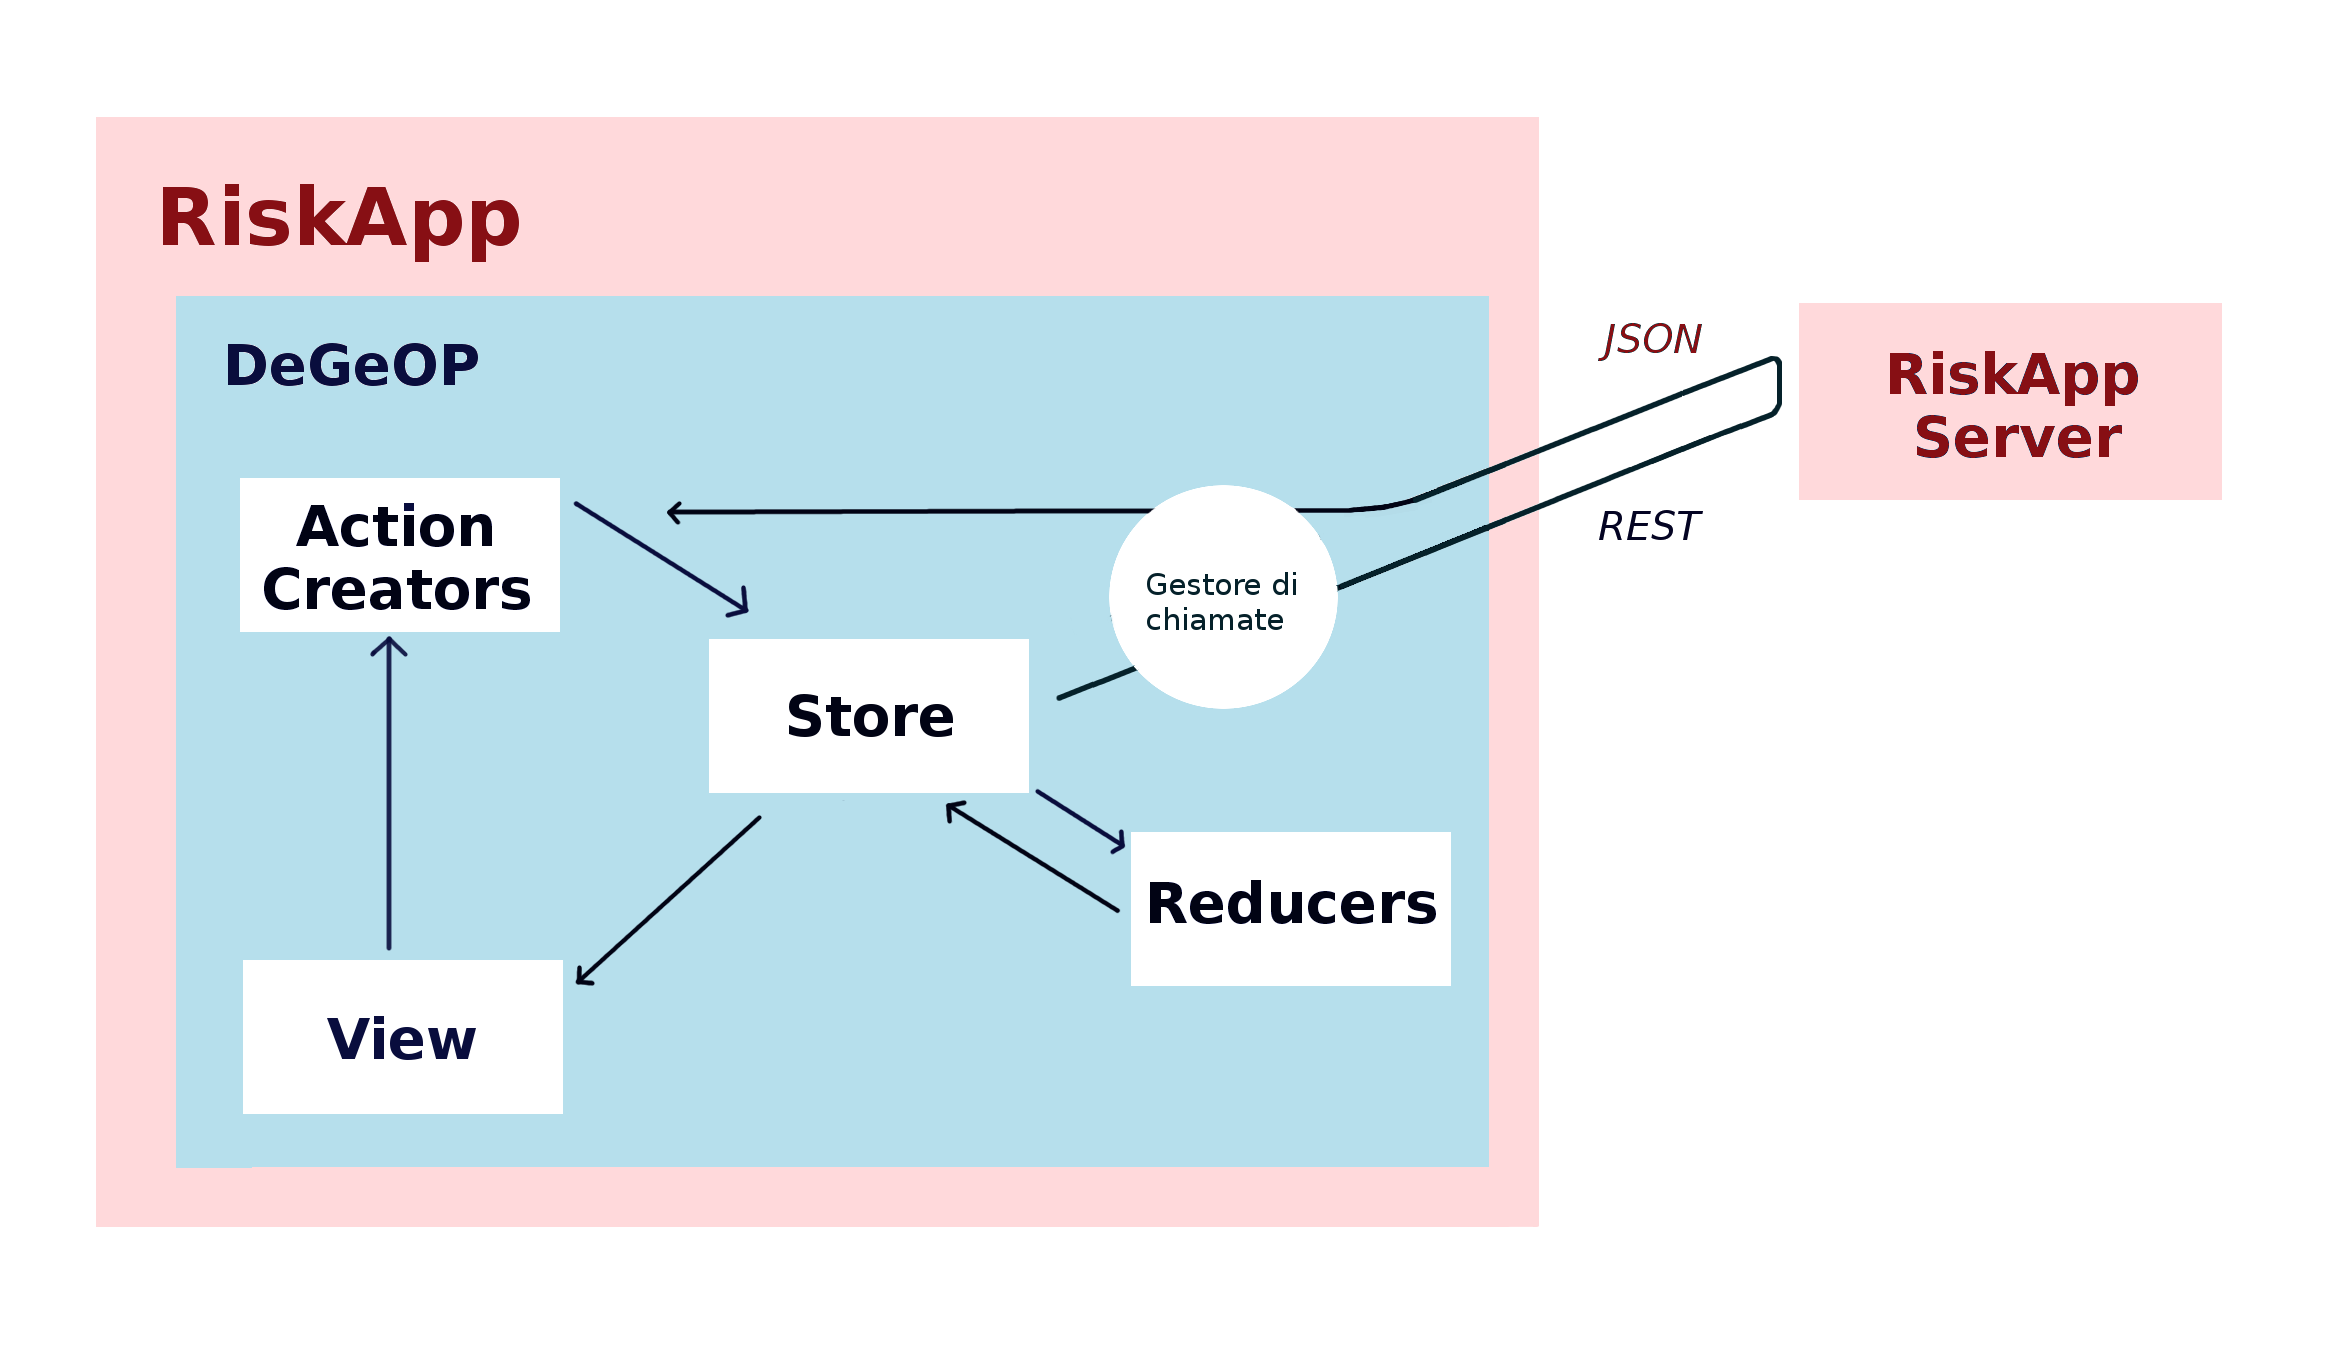
\includegraphics[width=\textwidth]{img/ArchitetturaBase.png}
	\caption{Architettura di base}
\end{figure}



	\section{Componenti} \label{componenti}
\subsection{DeGeOP}
\label{pkg::DeGeOP}
\begin{figure}[H]
	\centering
	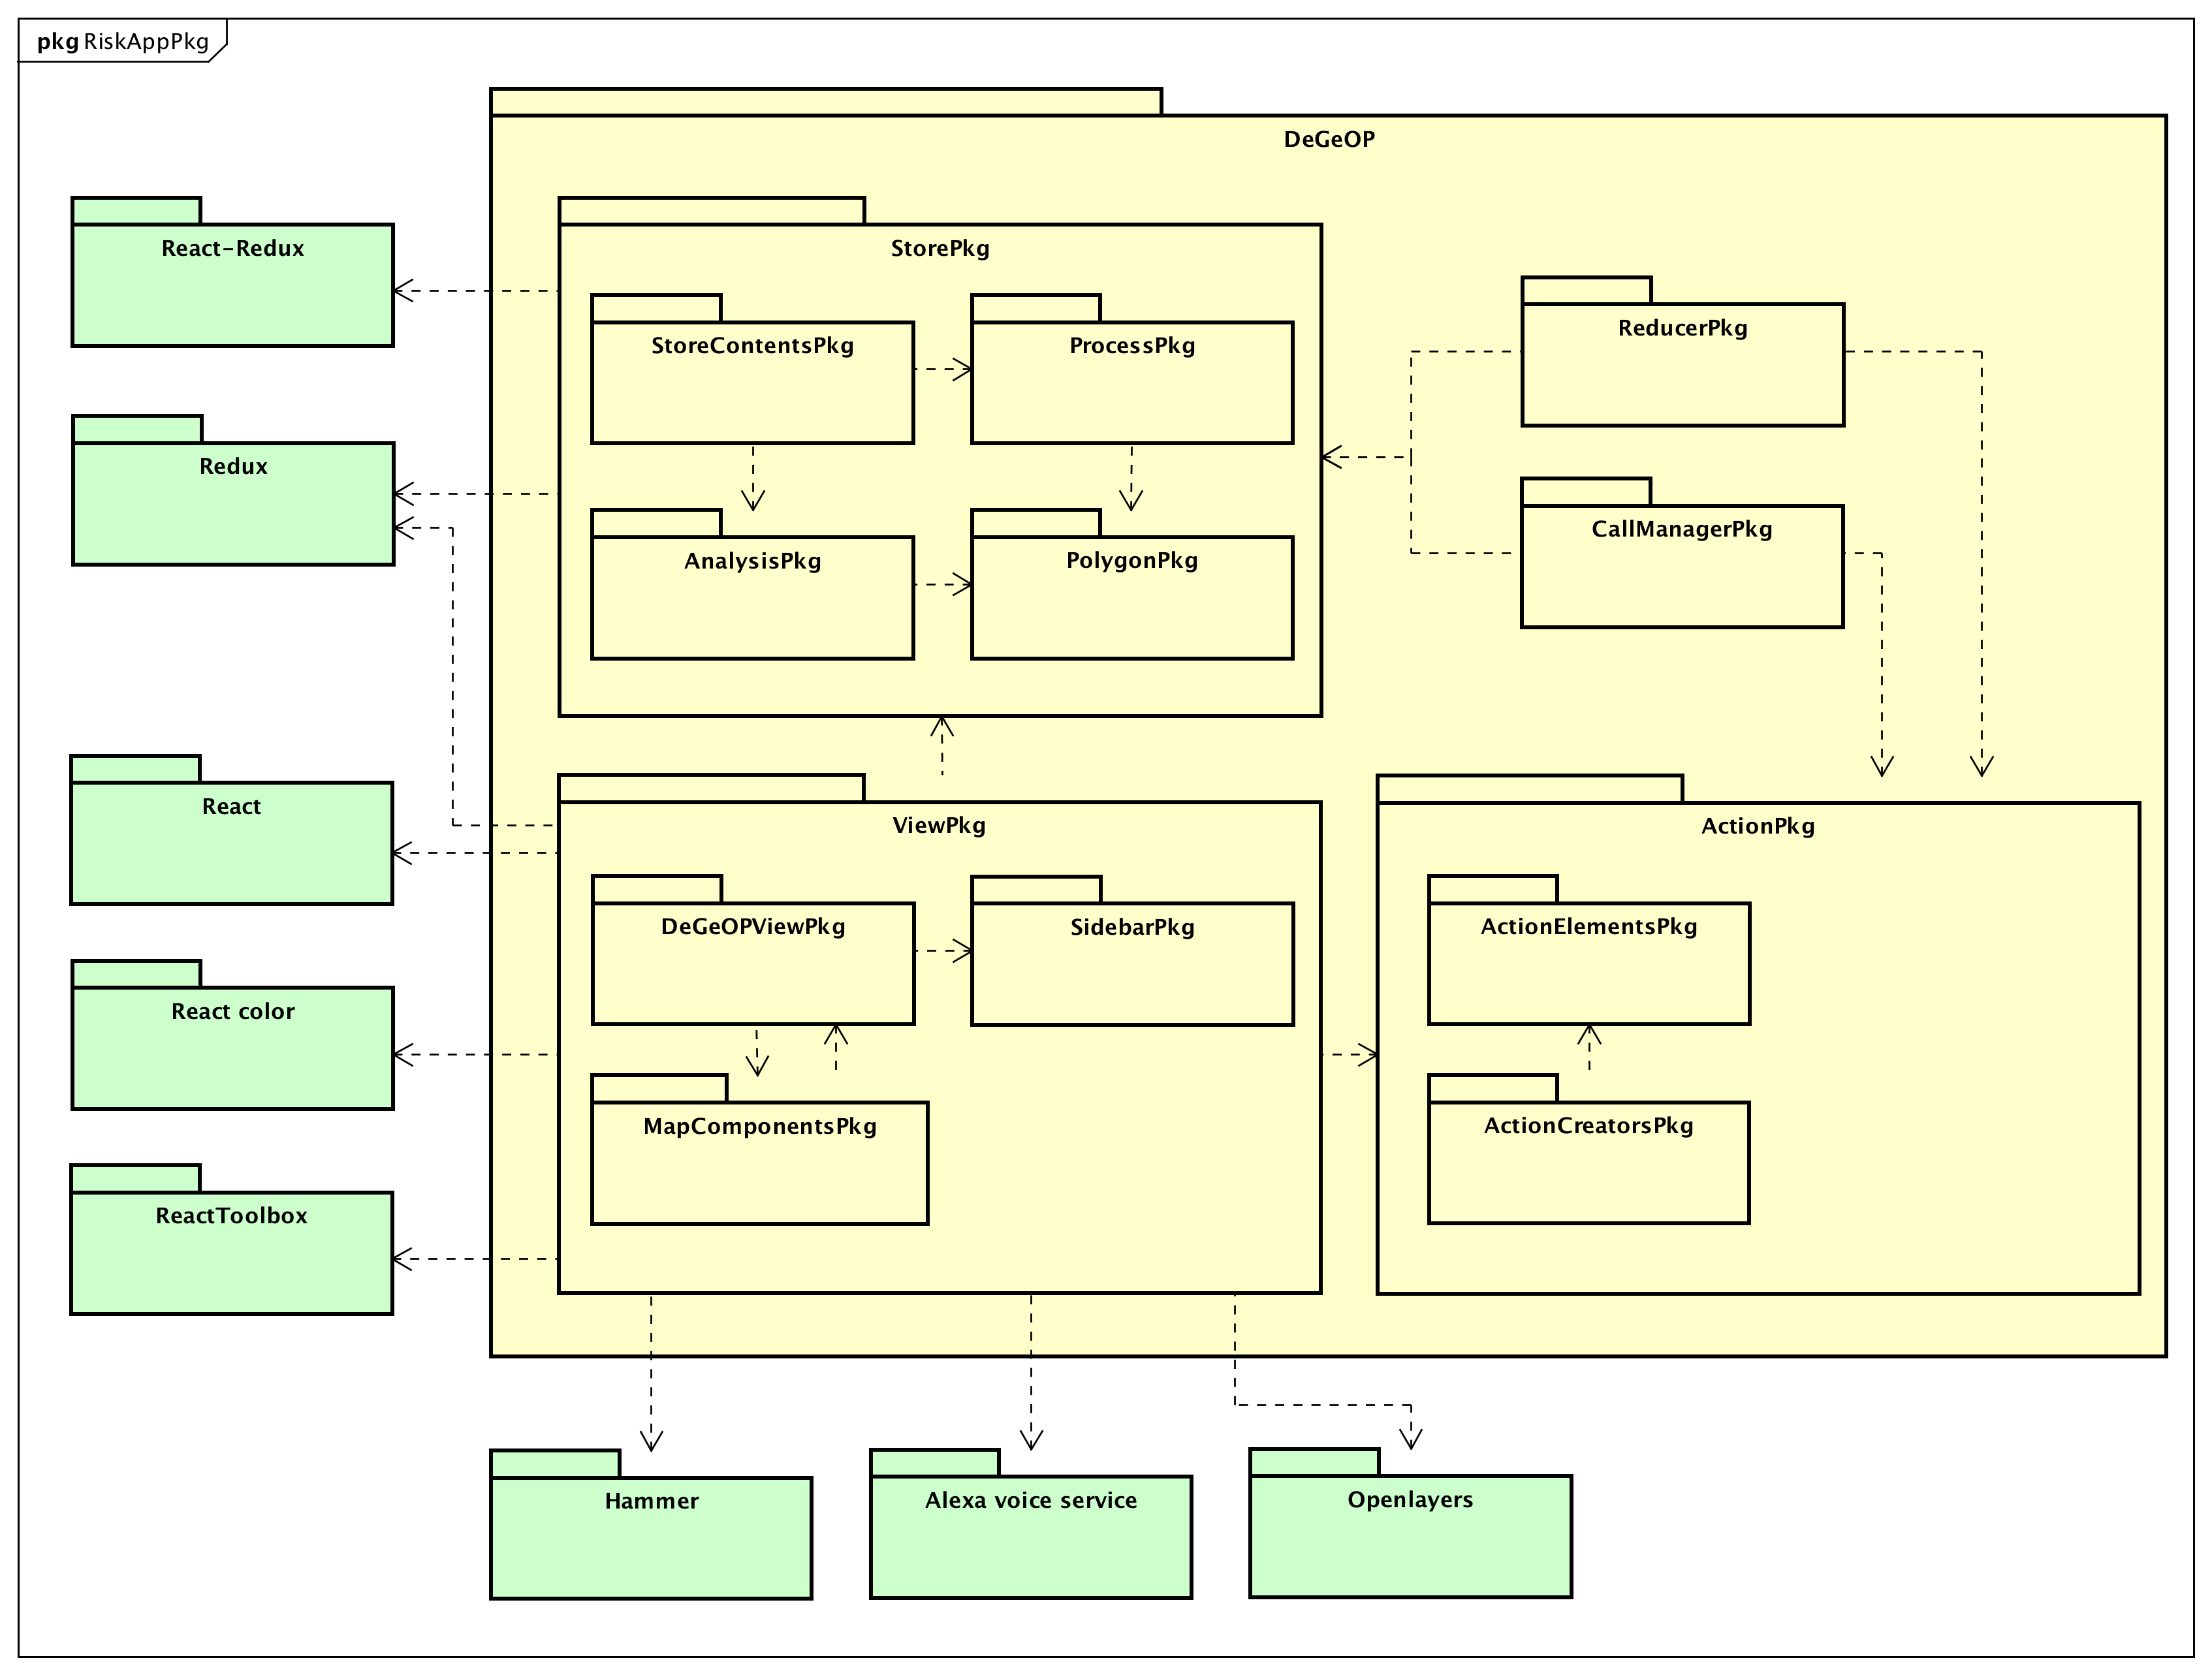
\includegraphics[width=\textwidth]{img/PkgDiagram/DeGeOPPkg.png}
	\caption{Schema componente DeGeOP}
\end{figure}
\subsubsection{Informazioni sul package}
\begin{itemize}
	\item \textbf{descrizione:} racchiude tutte le componenti necessarie per il front-end del prodotto;
	\item \textbf{\glo{Package}{package} contenuti:}
	\begin{itemize}
		\item DeGeOP::\hyperref[pkg::ActionPkg]{ActionPkg};
		\item DeGeOP::\hyperref[pkg::CallManagerPkg]{CallManagerPkg};
		\item DeGeOP::\hyperref[pkg::ReducerPkg]{ReducerPkg};
		\item DeGeOP::\hyperref[pkg::StorePkg]{StorePkg};
		\item DeGeOP::\hyperref[pkg::ViewPkg]{ViewPkg}.
	\end{itemize}
\end{itemize}
\newpage
\subsection{DeGeOP::StorePkg}
\label{pkg::StorePkg}
\begin{figure}[H]
	\centering
	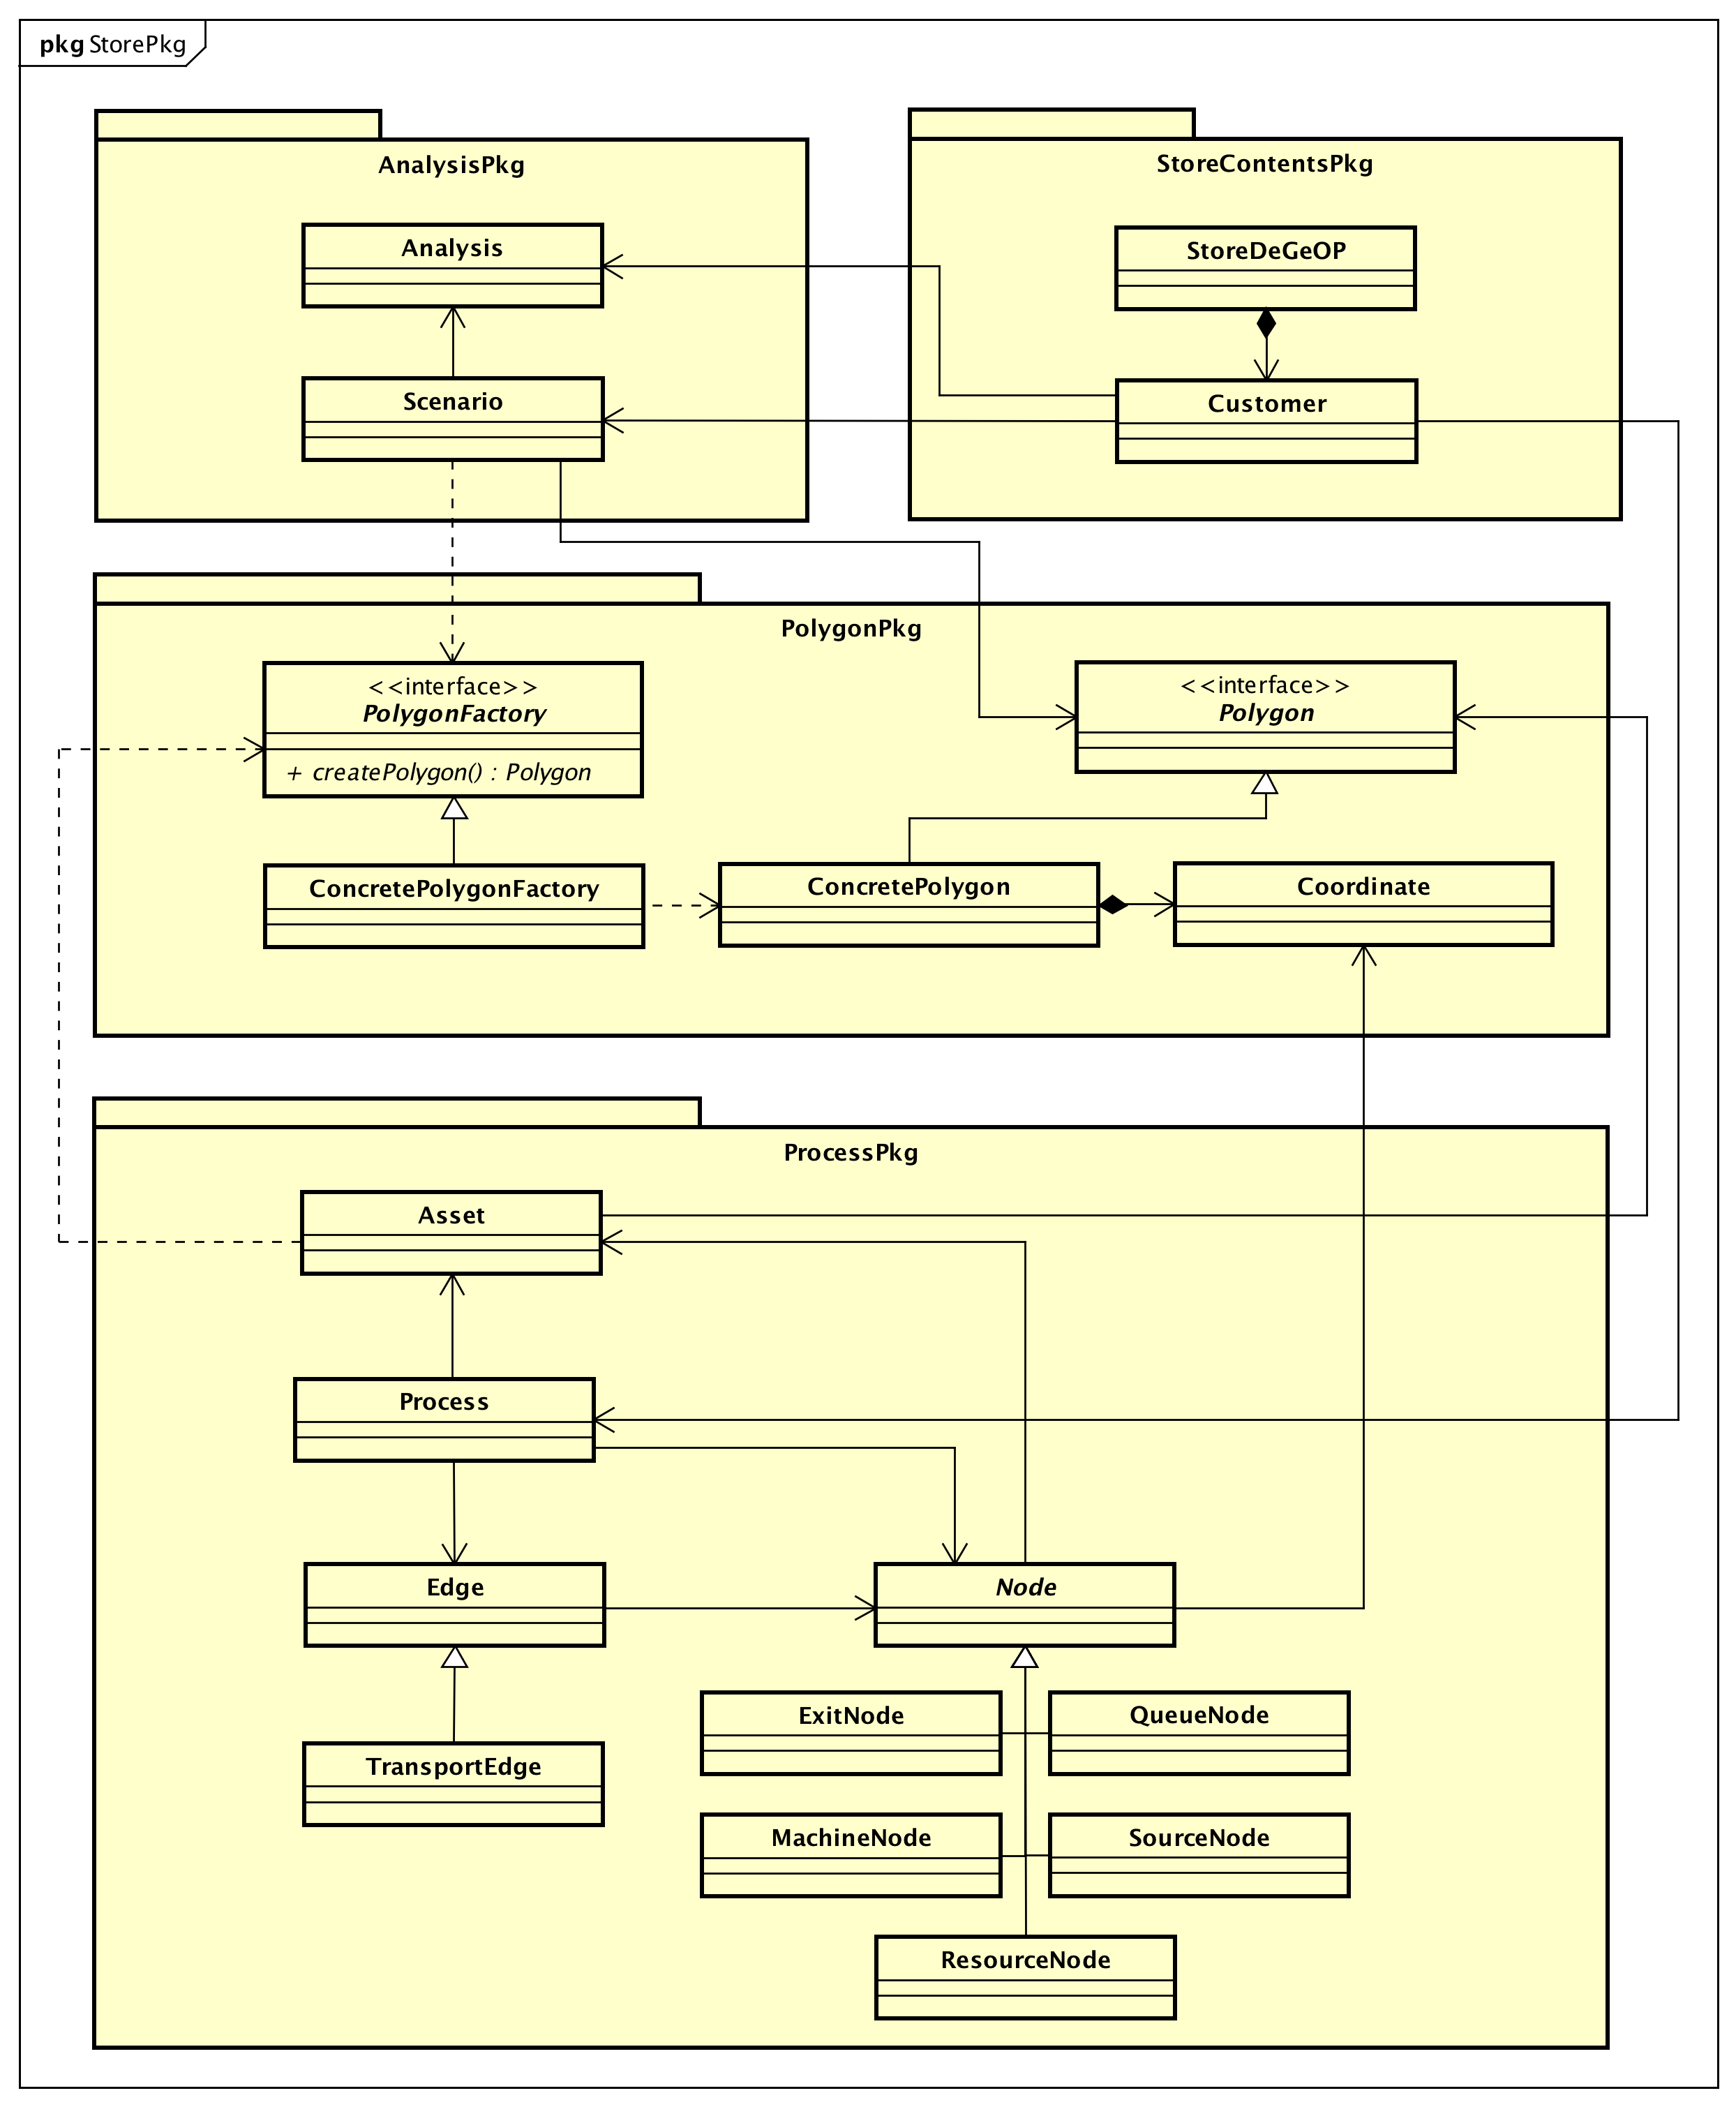
\includegraphics[width=\textwidth]{img/PkgDiagram/StorePkg.png}
	\caption{Schema componente DeGeOP::StorePkg}
\end{figure}
\subsubsection{Informazioni sul package}
\begin{itemize}
	\item \textbf{descrizione:} racchiude le componenti utilizzate per la memorizzazione e rappresentazione dei dati.;
	\item \textbf{padre:} \hyperref[pkg::DeGeOP]{DeGeOP};
	\item \textbf{package contenuti:}
	\begin{itemize}
		\item StorePkg::\hyperref[pkg::AnalysisPkg]{AnalysisPkg};
		\item StorePkg::\hyperref[pkg::PolygonPkg]{PolygonPkg};
		\item StorePkg::\hyperref[pkg::ProcessPkg]{ProcessPkg};
		\item StorePkg::\hyperref[pkg::StoreContentsPkg]{StoreContentsPkg}.
	\end{itemize}
	\item \textbf{interazioni con altri package:} 
	\begin{itemize}
		\item IN CallManagerPkg: subscribe sullo \glo{Store}{store};
		\item IN ReducerPkg: applicazione di cambiamenti di stato;
		\item IN ViewPkg: subscribe sullo store;
		\item OUT \glo{React}{React}-Redux: utilizzo di Provider per evitare di passare lo store come \glo{Proprietà}{proprietà} alle componenti React;
		\item OUT Redux: creazione Store utilizzando il metodo createStore().
	\end{itemize}
\end{itemize}
\newpage
\subsection{DeGeOP::StorePkg::StoreContentsPkg}
\label{pkg::StoreContentsPkg}
\subsubsection{Informazioni sul package}
\begin{itemize}
	\item \textbf{descrizione:} racchiude le componenti che implementano il concetto di store dell'architettura Redux.;
	\item \textbf{padre:} \hyperref[pkg::StorePkg]{StorePkg};
	\item \textbf{interazioni con altri package:} 
	\begin{itemize}
		\item OUT AnalysisPkg: riferimento ad analisi di danno;
		\item OUT ProcessPkg: riferimento a processo;
		\item OUT React-Redux: utilizzo del Provider;
		\item OUT Redux: creazione store.
	\end{itemize}
	\item \textbf{classi contenute:}
	\begin{itemize}
		\item Customer;
		\item StoreDeGeOP.
	\end{itemize}
\end{itemize}
\subsubsection{Classi}
\paragraph{Customer}
\begin{itemize}
	\item \textbf{descrizione:} rappresenta l'assicurando;
	\item \textbf{utilizzo:} viene utilizzato nello Store per memorizzare l'assicurando;
	\item \textbf{relazioni con altre classi:} 
	\begin{itemize}
		\item OUT Analysis;
		\item OUT Process;
		\item OUT Scenario.
	\end{itemize}
\end{itemize}
\paragraph{StoreDeGeOP}
\begin{itemize}
	\item \textbf{descrizione:} rappresenta una classe che incapsula uno Store creato utilizzando Redux;
	\item \textbf{utilizzo:} viene utilizzato per memorizzare lo stato dell'applicazione.
	Le componenti che effettuano il subscribe sullo Store verranno notificate ad ogni cambiamento di stato dello Store;
	\item \textbf{relazioni con altre classi:} 
	\begin{itemize}
		\item IN DeGeOPView.
	\end{itemize}
\end{itemize}
\newpage
\subsection{DeGeOP::StorePkg::ProcessPkg}
\label{pkg::ProcessPkg}
\subsubsection{Informazioni sul package}
\begin{itemize}
	\item \textbf{descrizione:} racchiude le componenti necessarie alla rappresentazione del processo produttivo dell'assicurando.;
	\item \textbf{padre:} \hyperref[pkg::StorePkg]{StorePkg};
	\item \textbf{interazioni con altri package:} 
	\begin{itemize}
		\item IN StoreContentsPkg: riferimento a processo;
		\item OUT PolygonPkg: riferimento ad un poligono.
	\end{itemize}
	\item \textbf{classi contenute:}
	\begin{itemize}
		\item \glo{Asset}{Asset};
		\item Edge;
		\item Exit;
		\item Machine;
		\item Node;
		\item Process;
		\item Queue;
		\item Resource;
		\item Source;
		\item TransportEdge.
	\end{itemize}
\end{itemize}
\subsubsection{Classi}
\paragraph{Asset}
\begin{itemize}
	\item \textbf{descrizione:} rappresenta un fabbricato di interesse per il processo produttivo dell'assicurando;
	\item \textbf{utilizzo:} sono contenuti all'interno di Process;
	\item \textbf{relazioni con altre classi:} 
	\begin{itemize}
		\item IN Node;
		\item IN Process;
		\item OUT Polygon;
		\item OUT PolygonFactory.
	\end{itemize}
\end{itemize}
\paragraph{Edge}
\begin{itemize}
	\item \textbf{descrizione:} rappresenta un \glo{Arco}{arco} che collega due \glo{Nodo}{nodi} tra di loro; un arco indica che i nodi sono in correlazione tra di loro;
	\item \textbf{utilizzo:} è contenuto all'interno di Process;
	\item \textbf{relazioni con altre classi:} 
	\begin{itemize}
		\item IN Process;
		\item IN \glo{Reducer}{Reducer}.
	\end{itemize}
\end{itemize}
\paragraph{Exit}
\begin{itemize}
	\item \textbf{descrizione:} rappresenta un nodo di tipo Uscita;
	\item \textbf{utilizzo:} è contenuto all'interno di Process.
\end{itemize}
\paragraph{Machine}
\begin{itemize}
	\item \textbf{descrizione:} rappresenta un nodo di tipo Macchina;
	\item \textbf{utilizzo:} è contenuto all'interno di Process.
\end{itemize}
\paragraph{Node}
\begin{itemize}
	\item \textbf{descrizione:} rappresenta un nodo contenuto all'interno di un Asset ;
	\item \textbf{utilizzo:} è contenuto all'interno di Process;
	\item \textbf{relazioni con altre classi:} 
	\begin{itemize}
		\item IN Process;
		\item IN Reducer;
		\item OUT Asset;
		\item OUT Coordinate.
	\end{itemize}
\end{itemize}
\paragraph{Process}
\begin{itemize}
	\item \textbf{descrizione:} rappresenta un processo produttivo dell'azienda dell'assicurando;
	\item \textbf{utilizzo:} è memorizzato nello Store;
	\item \textbf{relazioni con altre classi:} 
	\begin{itemize}
		\item IN Customer;
		\item OUT Asset;
		\item OUT Edge;
		\item OUT Node.
	\end{itemize}
\end{itemize}
\paragraph{Queue}
\begin{itemize}
	\item \textbf{descrizione:} rappresenta un nodo di tipo Coda;
	\item \textbf{utilizzo:} è contenuto all'interno di Process.
\end{itemize}
\paragraph{Resource}
\begin{itemize}
	\item \textbf{descrizione:} rappresenta un nodo di tipo Risorsa;
	\item \textbf{utilizzo:} è contenuto all'interno di Process.
\end{itemize}
\paragraph{Source}
\begin{itemize}
	\item \textbf{descrizione:} rappresenta un nodo di tipo Sorgente;
	\item \textbf{utilizzo:} è contenuto all'interno di Process.
\end{itemize}
\paragraph{TransportEdge}
\begin{itemize}
	\item \textbf{descrizione:} rappresenta un arco di tipo Trasporto;
	\item \textbf{utilizzo:} è contenuto all'interno di Process.
\end{itemize}
\newpage
\subsection{DeGeOP::StorePkg::AnalysisPkg}
\label{pkg::AnalysisPkg}
\subsubsection{Informazioni sul package}
\begin{itemize}
	\item \textbf{descrizione:} racchiude le componenti necessarie alla rappresentazione dell'analisi di danno relative al processo produttivo dell'assicurando. ;
	\item \textbf{padre:} \hyperref[pkg::StorePkg]{StorePkg};
	\item \textbf{interazioni con altri package:} 
	\begin{itemize}
		\item IN StoreContentsPkg: riferimento ad analisi di danno;
		\item OUT PolygonPkg: riferimento ad un poligono.
	\end{itemize}
	\item \textbf{classi contenute:}
	\begin{itemize}
		\item Analysis;
		\item Scenario.
	\end{itemize}
\end{itemize}
\subsubsection{Classi}
\paragraph{Analysis}
\begin{itemize}
	\item \textbf{descrizione:} rappresenta un risultato di un'analisi di danno relativo ad uno scenario;
	\item \textbf{utilizzo:} i metodi di questa classe saranno utilizzati per calcolare dati riassuntivi sull'analisi di danno;
	\item \textbf{relazioni con altre classi:} 
	\begin{itemize}
		\item IN Customer;
		\item IN Scenario.
	\end{itemize}
\end{itemize}
\paragraph{Scenario}
\begin{itemize}
	\item \textbf{descrizione:} rappresenta uno scenario di danno;
	\item \textbf{utilizzo:} viene utilizzata nello store per rappresentare gli scenari di danno;
	\item \textbf{relazioni con altre classi:} 
	\begin{itemize}
		\item IN Customer;
		\item IN Reducer;
		\item OUT Analysis;
		\item OUT Polygon;
		\item OUT PolygonFactory.
	\end{itemize}
\end{itemize}
\newpage
\subsection{DeGeOP::StorePkg::PolygonPkg}
\label{pkg::PolygonPkg}
\subsubsection{Informazioni sul package}
\begin{itemize}
	\item \textbf{descrizione:} racchiude le componenti necessarie alla rappresentazione dell'area degli asset e degli scenari di danno.;
	\item \textbf{padre:} \hyperref[pkg::StorePkg]{StorePkg};
	\item \textbf{interazioni con altri package:} 
	\begin{itemize}
		\item IN AnalysisPkg: riferimento ad un poligono;
		\item IN ProcessPkg: riferimento ad un poligono.
	\end{itemize}
	\item \textbf{classi contenute:}
	\begin{itemize}
		\item ConcretePolygon;
		\item ConcretePolygonFactory;
		\item Coordinate;
		\item Polygon;
		\item PolygonFactory.
	\end{itemize}
\end{itemize}
\subsubsection{Classi}
\paragraph{ConcretePolygon}
\begin{itemize}
	\item \textbf{descrizione:} rappresenta un poligono;
	\item \textbf{utilizzo:} viene istanziata da ConcretePolygonFactory; viene utilizzata in Asset e Scenario;
	\item \textbf{relazioni con altre classi:} 
	\begin{itemize}
		\item IN ConcretePolygonFactory;
		\item OUT Coordinate.
	\end{itemize}
\end{itemize}
\paragraph{ConcretePolygonFactory}
\begin{itemize}
	\item \textbf{descrizione:} gestisce la creazione concreta dei poligoni;
	\item \textbf{utilizzo:} implementazione di PolygonFactory; è la classe concreta da istanziare per gestire la creazione di un poligono;
	\item \textbf{relazioni con altre classi:} 
	\begin{itemize}
		\item OUT ConcretePolygon.
	\end{itemize}
\end{itemize}
\paragraph{Coordinate}
\begin{itemize}
	\item \textbf{descrizione:} rappresenta una coordinata geografica;
	\item \textbf{utilizzo:} è utilizzata all'interno di Polygon per delimitarne i suoi vertici;
	\item \textbf{relazioni con altre classi:} 
	\begin{itemize}
		\item IN ConcretePolygon;
		\item IN Node.
	\end{itemize}
\end{itemize}
\paragraph{Polygon}
\begin{itemize}
	\item \textbf{descrizione:} interfaccia che rappresenta il poligono;
	\item \textbf{utilizzo:} fornisce i metodi del poligono;
	\item \textbf{relazioni con altre classi:} 
	\begin{itemize}
		\item IN Asset;
		\item IN Scenario.
	\end{itemize}
\end{itemize}
\paragraph{PolygonFactory}
\begin{itemize}
	\item \textbf{descrizione:} interfaccia che si occupa della costruzione dei poligoni;
	\item \textbf{utilizzo:} viene usata dalle classi Scenario e Asset per la costruzione dei poligoni;
	\item \textbf{relazioni con altre classi:} 
	\begin{itemize}
		\item IN Asset;
		\item IN Scenario.
	\end{itemize}
\end{itemize}
\newpage
\subsection{DeGeOP::ReducerPkg}
\label{pkg::ReducerPkg}
\begin{figure}[H]
	\centering
	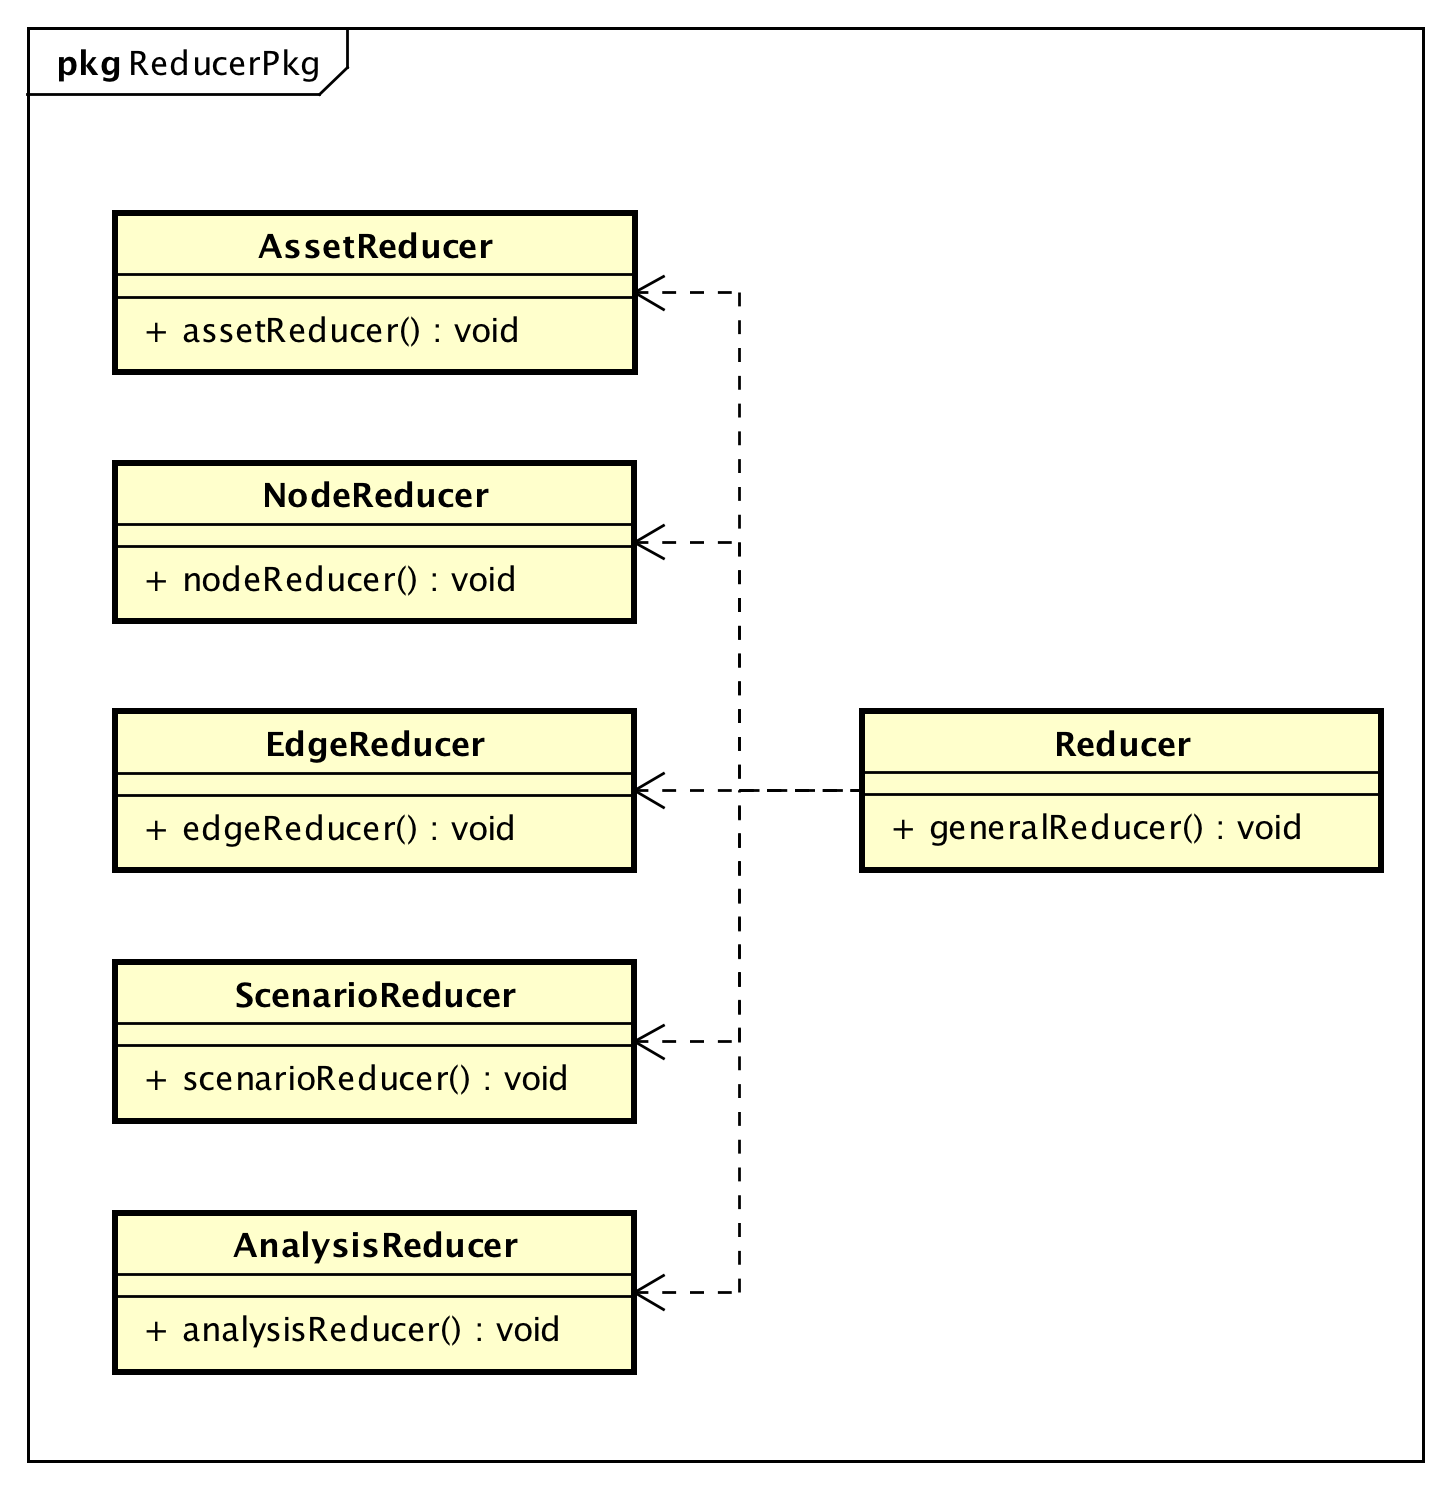
\includegraphics[width=\textwidth]{img/PkgDiagram/ReducerPkg.png}
	\caption{Schema componente DeGeOP::ReducerPkg}
\end{figure}
\subsubsection{Informazioni sul package}
\begin{itemize}
	\item \textbf{descrizione:} racchiude le componenti necessarie all'implementazione dei reducer secondo l'architettura Redux.;
	\item \textbf{padre:} \hyperref[pkg::DeGeOP]{DeGeOP};
	\item \textbf{interazioni con altri package:} 
	\begin{itemize}
		\item OUT ActionPkg: utilizzo di azioni ;
		\item OUT StorePkg: applicazione di cambiamenti di stato.
	\end{itemize}
	\item \textbf{classi contenute:}
	\begin{itemize}
		\item AnalysisReducer;
		\item AssetReducer;
		\item EdgeReducer;
		\item NodeReducer;
		\item Reducer;
		\item ScenarioReducer.
	\end{itemize}
\end{itemize}
\subsubsection{Classi}
\paragraph{AnalysisReducer}
\begin{itemize}
	\item \textbf{descrizione:} rappresenta il reducer dell'analisi;
	\item \textbf{utilizzo:} il suo metodo gestisce le operazioni sullo store riguardanti le analisi;
	\item \textbf{relazioni con altre classi:} 
	\begin{itemize}
		\item IN Reducer.
	\end{itemize}
\end{itemize}
\paragraph{AssetReducer}
\begin{itemize}
	\item \textbf{descrizione:} rappresenta il reducer dell'asset;
	\item \textbf{utilizzo:} il suo metodo gestisce le operazioni sullo store riguardanti l'asset;
	\item \textbf{relazioni con altre classi:} 
	\begin{itemize}
		\item IN Reducer.
	\end{itemize}
\end{itemize}
\paragraph{EdgeReducer}
\begin{itemize}
	\item \textbf{descrizione:} rappresenta il reducer dell'arco;
	\item \textbf{utilizzo:} il suo metodo gestisce le operazioni sullo store riguardanti gli archi.
\end{itemize}
\paragraph{NodeReducer}
\begin{itemize}
	\item \textbf{descrizione:} rappresenta il reducer del nodo;
	\item \textbf{utilizzo:} il suo metodo gestisce le operazioni sullo store riguardanti i nodi.
\end{itemize}
\paragraph{Reducer}
\begin{itemize}
	\item \textbf{descrizione:} accetta una \glo{Action}{action} generica in input e la reindirizza al giusto reducer;
	\item \textbf{utilizzo:} il suo metodo viene utilizzato per catturare un'azione e generare un nuovo stato sullo Store;
	\item \textbf{relazioni con altre classi:} 
	\begin{itemize}
		\item OUT AnalysisReducer;
		\item OUT AssetReducer;
		\item OUT Edge;
		\item OUT Node;
		\item OUT Scenario.
	\end{itemize}
\end{itemize}
\paragraph{ScenarioReducer}
\begin{itemize}
	\item \textbf{descrizione:} rappresenta il reducer dello scenario;
	\item \textbf{utilizzo:} il suo metodo gestisce le operazioni sullo store riguardanti gli scenari.
\end{itemize}
\newpage
\subsection{DeGeOP::CallManagerPkg}
\label{pkg::CallManagerPkg}
\begin{figure}[H]
	\centering
	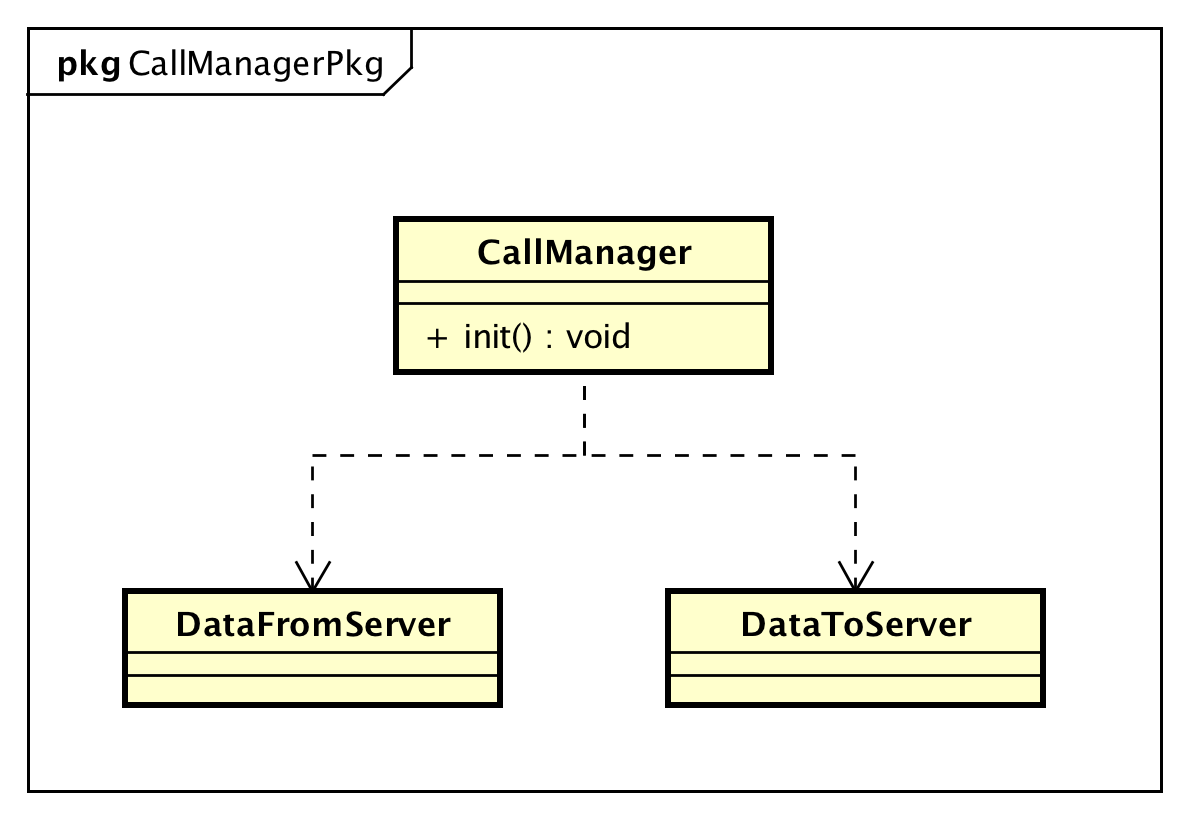
\includegraphics[width=\textwidth]{img/PkgDiagram/CallManagerPkg.png}
	\caption{Schema componente DeGeOP::CallManagerPkg}
\end{figure}
\subsubsection{Informazioni sul package}
\begin{itemize}
	\item \textbf{descrizione:} racchiude le componenti necessarie alla comunicazione dei dati verso il server;
	\item \textbf{padre:} \hyperref[pkg::DeGeOP]{DeGeOP};
	\item \textbf{interazioni con altri package:} 
	\begin{itemize}
		\item OUT ActionPkg: \glo{Dispatch}{dispatch} di azioni;
		\item OUT StorePkg: subscribe sullo store.
	\end{itemize}
	\item \textbf{classi contenute:}
	\begin{itemize}
		\item CallManager;
		\item DataFromServer;
		\item DataToServer.
	\end{itemize}
\end{itemize}
\subsubsection{Classi}
\paragraph{CallManager}
\begin{itemize}
	\item \textbf{descrizione:} rappresenta il gestore delle chiamate da e verso il server;
	\item \textbf{utilizzo:} viene usato per effettuare chiamate REST da e verso il server. I suoi metodi si occupano di inizializzare lo Store emettendo Action quando l'applicazione viene aperta. Sfrutta i metodi della classe DataFromServer per effettuare la conversione da JSON ad oggetto logico. Inoltre, la classe effettuerà il subscribe allo Store per ricevere i cambiamenti di stato e mantenere aggiornate le informazioni sul server. La classe avrà un metodo che identifica cos'è cambiato nello Store e farà la chiamata REST appropriata, sfruttando la classe DataToServer per trasformare l'oggetto logico in JSON;
	\item \textbf{relazioni con altre classi:} 
	\begin{itemize}
		\item OUT AnalysisActionCreator;
		\item OUT AssetActionCreator;
		\item OUT DataFromServer;
		\item OUT DataToServer;
		\item OUT EdgeActionCreator;
		\item OUT NodeActionCreator;
		\item OUT ScenarioActionCreator.
	\end{itemize}
\end{itemize}
\paragraph{DataFromServer}
\begin{itemize}
	\item \textbf{descrizione:} rappresenta il gestore dei dati ricevuti dal server;
	\item \textbf{utilizzo:} gestisce i dati ricevuti dal server. I suoi metodi si occupano di effettuare la conversione dei JSON ricevuti dal server in oggetti logici;
	\item \textbf{relazioni con altre classi:} 
	\begin{itemize}
		\item IN CallManager.
	\end{itemize}
\end{itemize}
\paragraph{DataToServer}
\begin{itemize}
	\item \textbf{descrizione:} rappresenta il gestore dei dati da inviare verso il server;
	\item \textbf{utilizzo:} gestisce i dati che dovranno essere inviati al server. I suoi metodi effettuano la conversione degli oggetti logici in JSON;
	\item \textbf{relazioni con altre classi:} 
	\begin{itemize}
		\item IN CallManager.
	\end{itemize}
\end{itemize}
\newpage
\subsection{DeGeOP::ActionPkg}
\label{pkg::ActionPkg}
\begin{figure}[H]
	\centering
	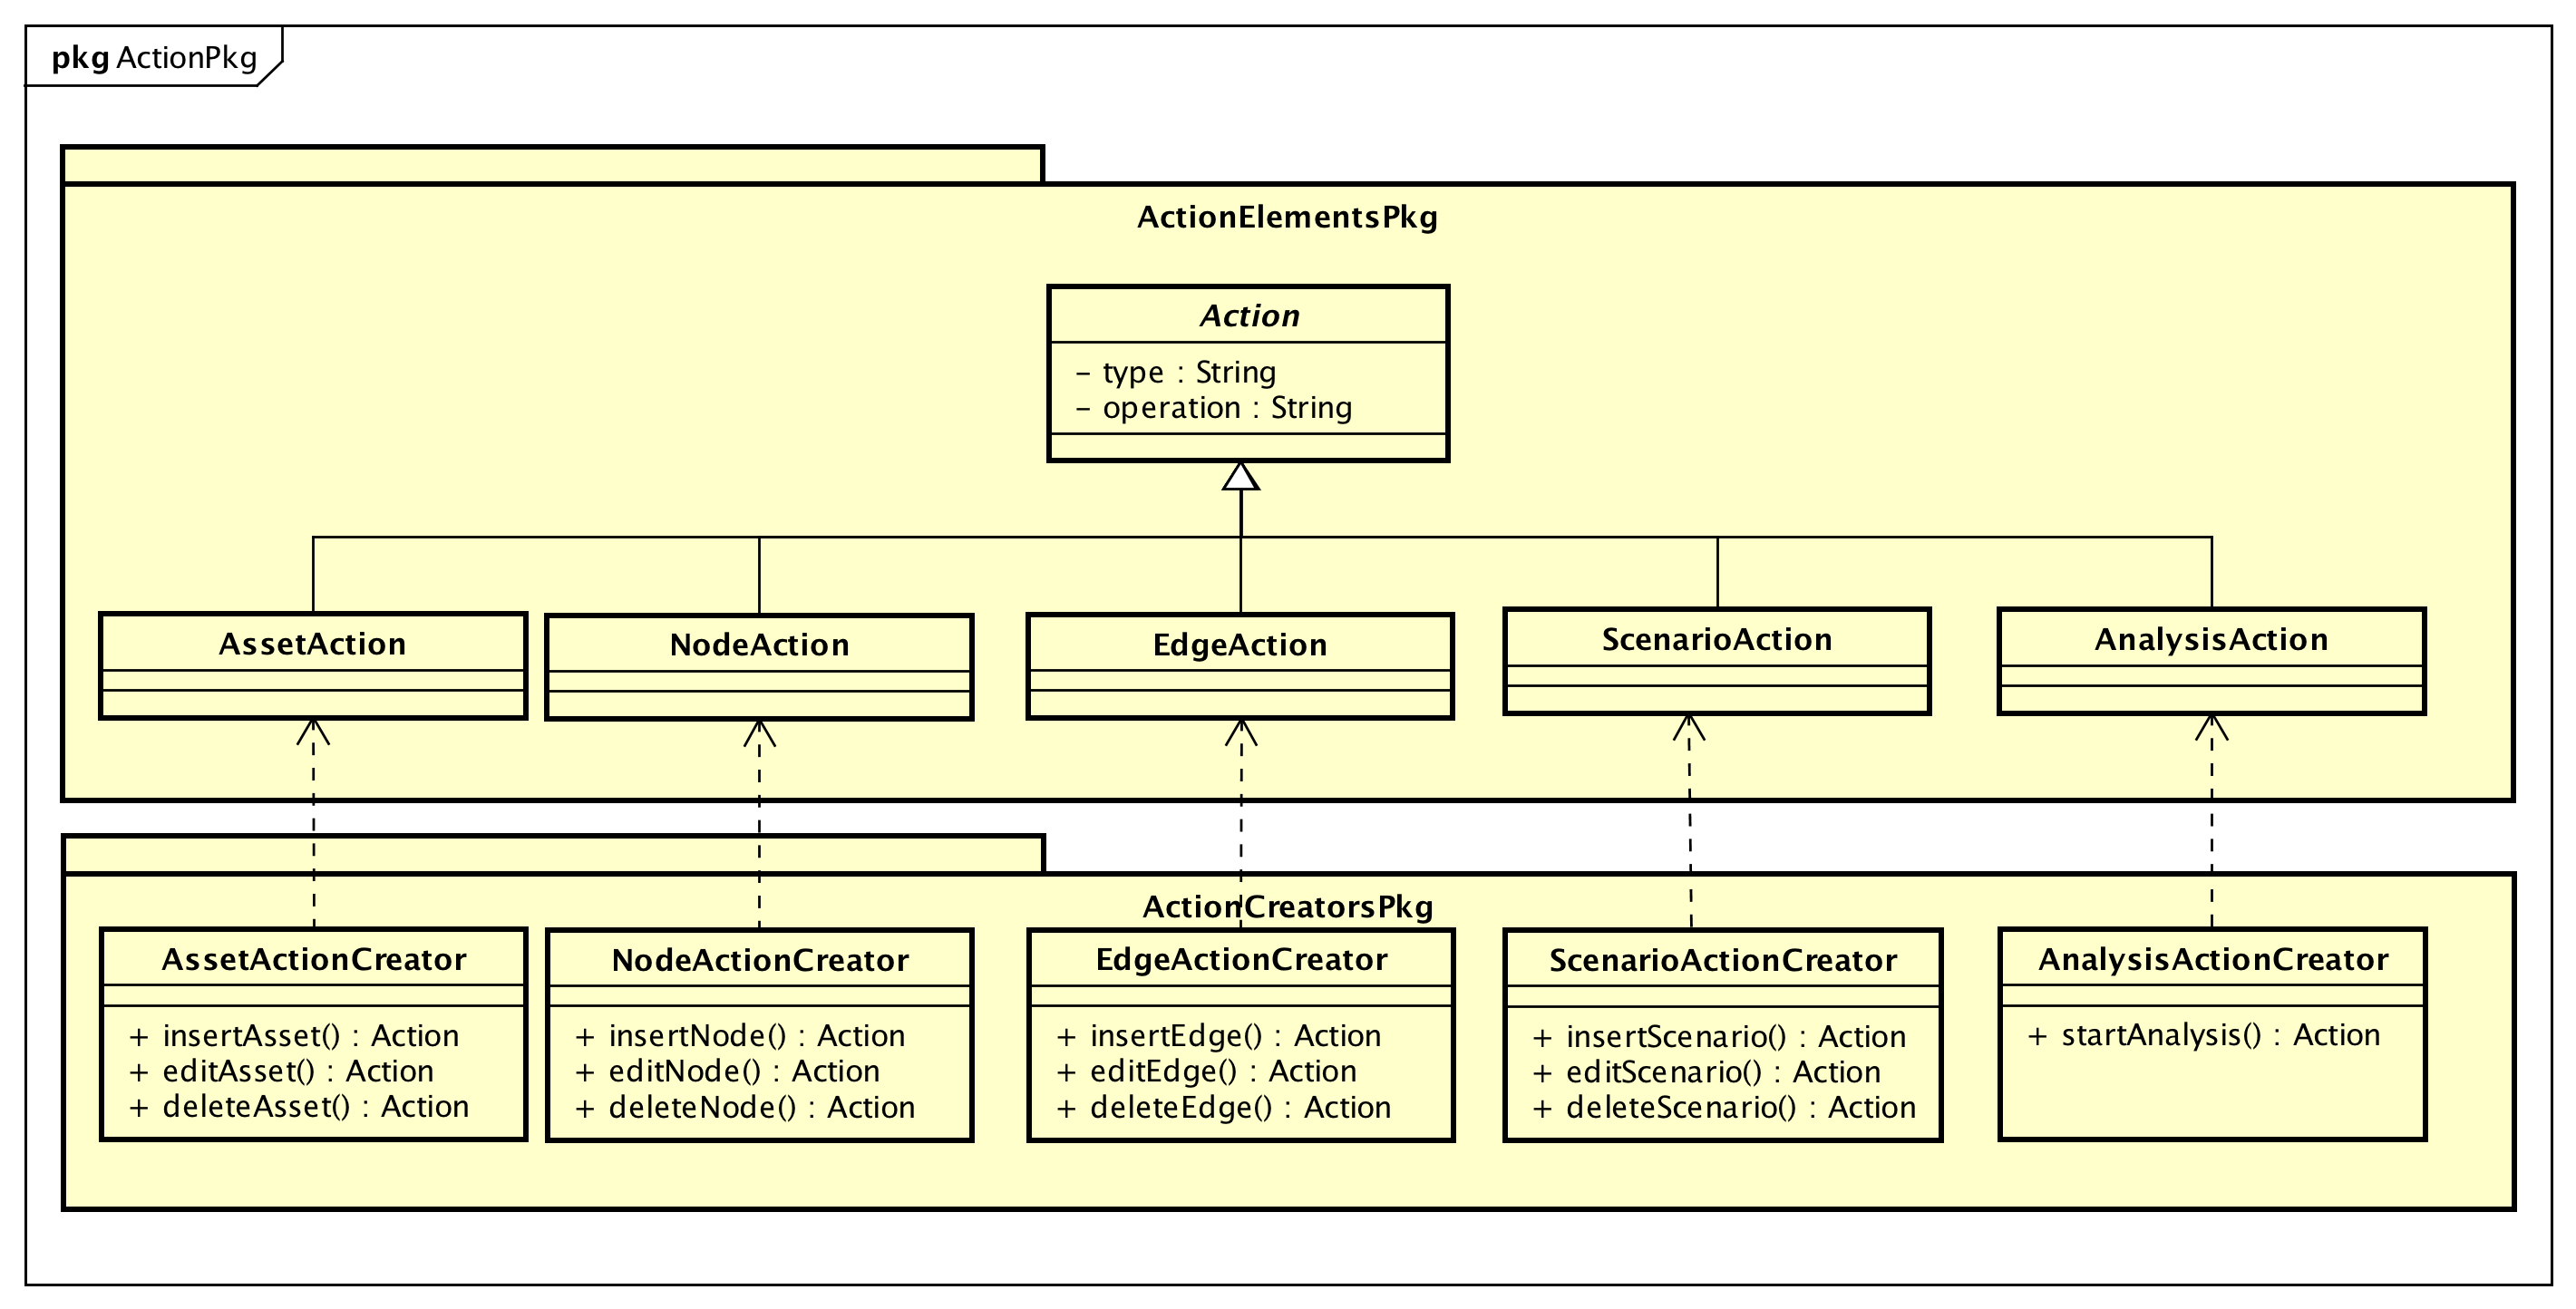
\includegraphics[width=\textwidth]{img/PkgDiagram/ActionPkg.png}
	\caption{Schema componente DeGeOP::ActionPkg}
\end{figure}
\subsubsection{Informazioni sul package}
\begin{itemize}
	\item \textbf{descrizione:} racchiude le componenti utilizzate per implementare le action dell'architettura Redux. Le action vengono create e ne viene fatto il dispatch verso lo store. Un reducer gestirà una action per produrre un cambiamento di stato sullo store.;
	\item \textbf{padre:} \hyperref[pkg::DeGeOP]{DeGeOP};
	\item \textbf{package contenuti:}
	\begin{itemize}
		\item ActionPkg::\hyperref[pkg::ActionCreatorsPkg]{ActionCreatorsPkg};
		\item ActionPkg::\hyperref[pkg::ActionElementsPkg]{ActionElementsPkg}.
	\end{itemize}
	\item \textbf{interazioni con altri package:} 
	\begin{itemize}
		\item IN CallManagerPkg: dispatch di azioni;
		\item IN ReducerPkg: utilizzo di azioni ;
		\item IN ViewPkg: dispatch di azioni.
	\end{itemize}
	\item \textbf{classi contenute:}
	\begin{itemize}
		\item EdgeAction.
	\end{itemize}
\end{itemize}
\subsubsection{Classi}
\paragraph{EdgeAction}
\begin{itemize}
	\item \textbf{descrizione:} rappresenta un'azione relativa agli archi;
	\item \textbf{utilizzo:} l'azione viene creata da un apposito ActionCreator per essere poi inviata ad un reducer;
	\item \textbf{relazioni con altre classi:} 
	\begin{itemize}
		\item IN EdgeActionCreator.
	\end{itemize}
\end{itemize}
\newpage
\subsection{DeGeOP::ActionPkg::ActionElementsPkg}
\label{pkg::ActionElementsPkg}
\subsubsection{Informazioni sul package}
\begin{itemize}
	\item \textbf{descrizione:} racchiude le componenti che rappresentano effettivamente le azioni;
	\item \textbf{padre:} \hyperref[pkg::ActionPkg]{ActionPkg};
	\item \textbf{interazioni con altri package:} 
	\begin{itemize}
		\item IN ActionCreatorsPkg: creazione di azioni.
	\end{itemize}
	\item \textbf{classi contenute:}
	\begin{itemize}
		\item Action;
		\item AnalysisAction;
		\item AssetAction;
		\item NodeAction;
		\item ScenarioAction.
	\end{itemize}
\end{itemize}
\subsubsection{Classi}
\paragraph{Action}
\begin{itemize}
	\item \textbf{descrizione:} una classe astratta che rappresenta una generica azione di cui può essere fatto il dispatch;
	\item \textbf{utilizzo:} i suoi membri vengono usati dai reducer per completare una azione.
\end{itemize}
\paragraph{AnalysisAction}
\begin{itemize}
	\item \textbf{descrizione:} rappresenta un'azione relativa alle analisi di danno;
	\item \textbf{utilizzo:} l'azione viene creata da un apposito ActionCreator per essere poi inviata ad un reducer;
	\item \textbf{relazioni con altre classi:} 
	\begin{itemize}
		\item IN AnalysisActionCreator.
	\end{itemize}
\end{itemize}
\paragraph{AssetAction}
\begin{itemize}
	\item \textbf{descrizione:} rappresenta un'azione relativa agli asset;
	\item \textbf{utilizzo:} l'azione viene creata da un apposito ActionCreator per essere poi inviata ad un reducer;
	\item \textbf{relazioni con altre classi:} 
	\begin{itemize}
		\item IN AssetActionCreator.
	\end{itemize}
\end{itemize}
\paragraph{NodeAction}
\begin{itemize}
	\item \textbf{descrizione:} rappresenta un'azione relativa ai nodi;
	\item \textbf{utilizzo:} l'azione viene creata da un apposito ActionCreator per essere poi inviata ad un reducer;
	\item \textbf{relazioni con altre classi:} 
	\begin{itemize}
		\item IN NodeActionCreator.
	\end{itemize}
\end{itemize}
\paragraph{ScenarioAction}
\begin{itemize}
	\item \textbf{descrizione:} rappresenta un'azione relativa agli scenari di danno;
	\item \textbf{utilizzo:} l'azione viene creata da un apposito ActionCreator per essere poi inviata ad un reducer;
	\item \textbf{relazioni con altre classi:} 
	\begin{itemize}
		\item IN ScenarioActionCreator.
	\end{itemize}
\end{itemize}
\newpage
\subsection{DeGeOP::ActionPkg::ActionCreatorsPkg}
\label{pkg::ActionCreatorsPkg}
\subsubsection{Informazioni sul package}
\begin{itemize}
	\item \textbf{descrizione:} racchiude le componenti che gestiscono la creazione delle azioni;
	\item \textbf{padre:} \hyperref[pkg::ActionPkg]{ActionPkg};
	\item \textbf{interazioni con altri package:} 
	\begin{itemize}
		\item OUT ActionElementsPkg: creazione di azioni.
	\end{itemize}
	\item \textbf{classi contenute:}
	\begin{itemize}
		\item AnalysisActionCreator;
		\item AssetActionCreator;
		\item EdgeActionCreator;
		\item NodeActionCreator;
		\item ScenarioActionCreator.
	\end{itemize}
\end{itemize}
\subsubsection{Classi}
\paragraph{AnalysisActionCreator}
\begin{itemize}
	\item \textbf{descrizione:} rappresenta la factory di azioni relative alle analisi di danno;
	\item \textbf{utilizzo:} i suoi metodi sono chiamati dalla View e dal CallManager per la creazione di azioni relative alle analisi di danno;
	\item \textbf{relazioni con altre classi:} 
	\begin{itemize}
		\item IN AnalysisButtons;
		\item IN CallManager;
		\item OUT AnalysisAction.
	\end{itemize}
\end{itemize}
\paragraph{AssetActionCreator}
\begin{itemize}
	\item \textbf{descrizione:} rappresenta la factory di azioni relative agli asset;
	\item \textbf{utilizzo:} i suoi metodi sono chiamati dalla View e dal CallManager per la creazione di azioni relative agli asset;
	\item \textbf{relazioni con altre classi:} 
	\begin{itemize}
		\item IN CallManager;
		\item IN EditAssetButtons;
		\item IN InsertAssetButtons;
		\item IN ViewAssetButtons;
		\item OUT AssetAction.
	\end{itemize}
\end{itemize}
\paragraph{EdgeActionCreator}
\begin{itemize}
	\item \textbf{descrizione:} rappresenta la factory di azioni relative agli archi;
	\item \textbf{utilizzo:} i suoi metodi sono chiamati dalla View e dal CallManager per la creazione di azioni relative agli archi;
	\item \textbf{relazioni con altre classi:} 
	\begin{itemize}
		\item IN CallManager;
		\item IN EditEdgeButtons;
		\item IN InsertEdgeButtons;
		\item IN ViewEdgeButtons;
		\item OUT EdgeAction.
	\end{itemize}
\end{itemize}
\paragraph{NodeActionCreator}
\begin{itemize}
	\item \textbf{descrizione:} rappresenta la factory di azioni relative ai nodi;
	\item \textbf{utilizzo:} i suoi metodi sono chiamati dalla View e dal CallManager per la creazione di azioni relative ai nodi;
	\item \textbf{relazioni con altre classi:} 
	\begin{itemize}
		\item IN CallManager;
		\item IN EditNodeButtons;
		\item IN InsertNodeButtons;
		\item IN ViewNodeButtons;
		\item OUT NodeAction.
	\end{itemize}
\end{itemize}
\paragraph{ScenarioActionCreator}
\begin{itemize}
	\item \textbf{descrizione:} rappresenta la factory di azioni relative agli scenari di danno;
	\item \textbf{utilizzo:} i suoi metodi sono chiamati dalla View e dal CallManager per la creazione di azioni relative agli scenari di danno;
	\item \textbf{relazioni con altre classi:} 
	\begin{itemize}
		\item IN CallManager;
		\item IN EditScenarioButtons;
		\item IN InsertScenarioButtons;
		\item IN ViewScenarioButtons;
		\item OUT ScenarioAction.
	\end{itemize}
\end{itemize}
\newpage
\subsection{DeGeOP::ViewPkg}
\label{pkg::ViewPkg}
\begin{figure}[H]
	\centering
	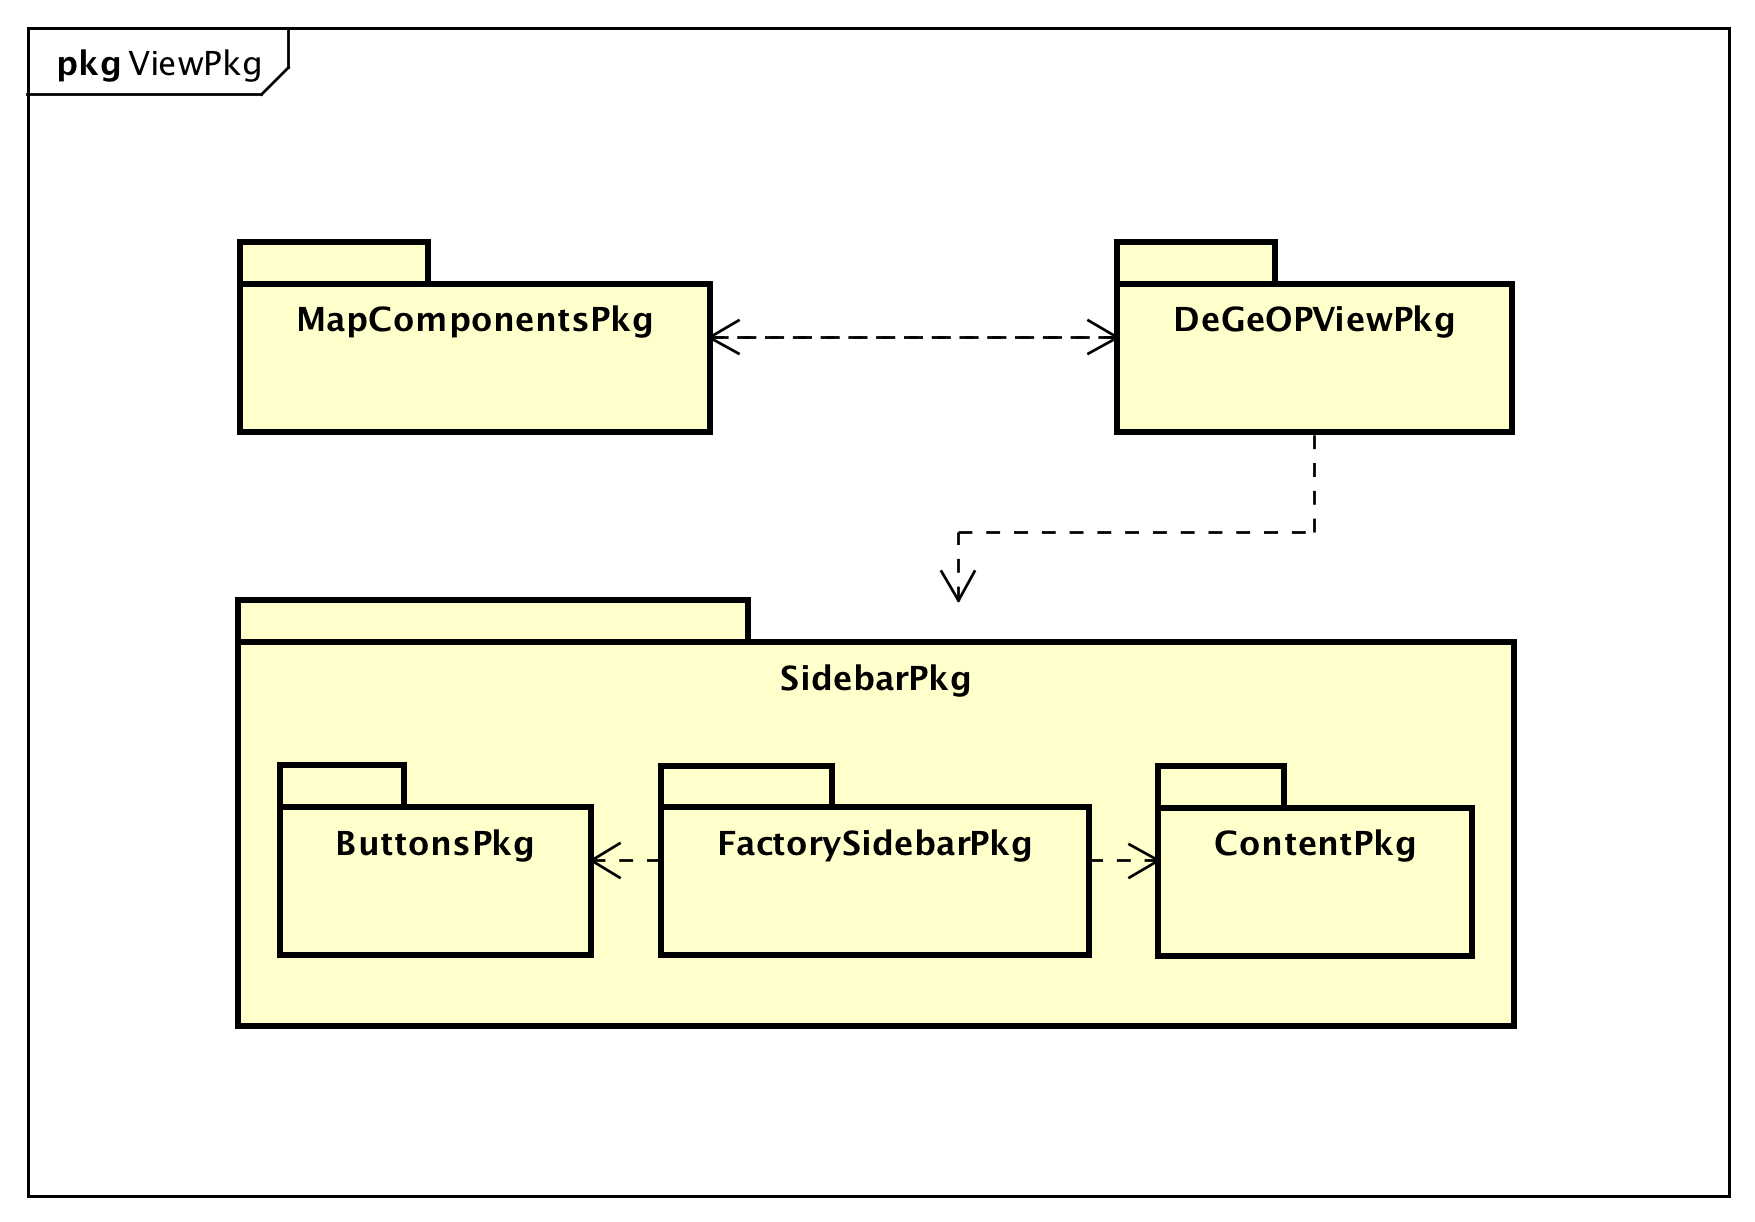
\includegraphics[width=\textwidth]{img/PkgDiagram/ViewPkg.png}
	\caption{Schema componente DeGeOP::ViewPkg}
\end{figure}
\subsubsection{Informazioni sul package}
\begin{itemize}
	\item \textbf{descrizione:} racchiude le componenti per la visualizzazione dell'interfaccia utente;
	\item \textbf{padre:} \hyperref[pkg::DeGeOP]{DeGeOP};
	\item \textbf{package contenuti:}
	\begin{itemize}
		\item ViewPkg::\hyperref[pkg::DeGeOPViewPkg]{DeGeOPViewPkg};
		\item ViewPkg::\hyperref[pkg::MapComponentsPkg]{MapComponentsPkg};
		\item ViewPkg::\hyperref[pkg::SidebarPkg]{SidebarPkg}.
	\end{itemize}
	
	\item \textbf{interazioni con altri package:} 
	\begin{itemize}
		\item OUT ActionPkg: dispatch di azioni;
		\item OUT Alexa voice service: gestore vocale;
		\item OUT Hammer: gestione gesture ;
		\item OUT Openlayers: gestione mappa;
		\item OUT React: utilizzo componenti react;
		\item OUT ReactToolbox: utilizzo componenti material design;
		\item OUT Redux: utilizzo metodo dispatch;
		\item OUT StorePkg: subscribe sullo store.
	\end{itemize}
	Il package presenta una dipendenza circolare con MapComponentsPkg. Tuttavia tale dipendenza viene risolta tramite l'utilizzo di un builder che inizializza l'oggetto DeGeOPView costruendo le sue parti. Inoltre, un verso della dipendenza è una dipendenza lasca, quindi non sono stati rilevati problemi da tale dipendenza circolare.
\end{itemize}
\newpage
\subsection{DeGeOP::ViewPkg::DeGeOPViewPkg}
\label{pkg::DeGeOPViewPkg}
\begin{figure}[H]
	\centering
	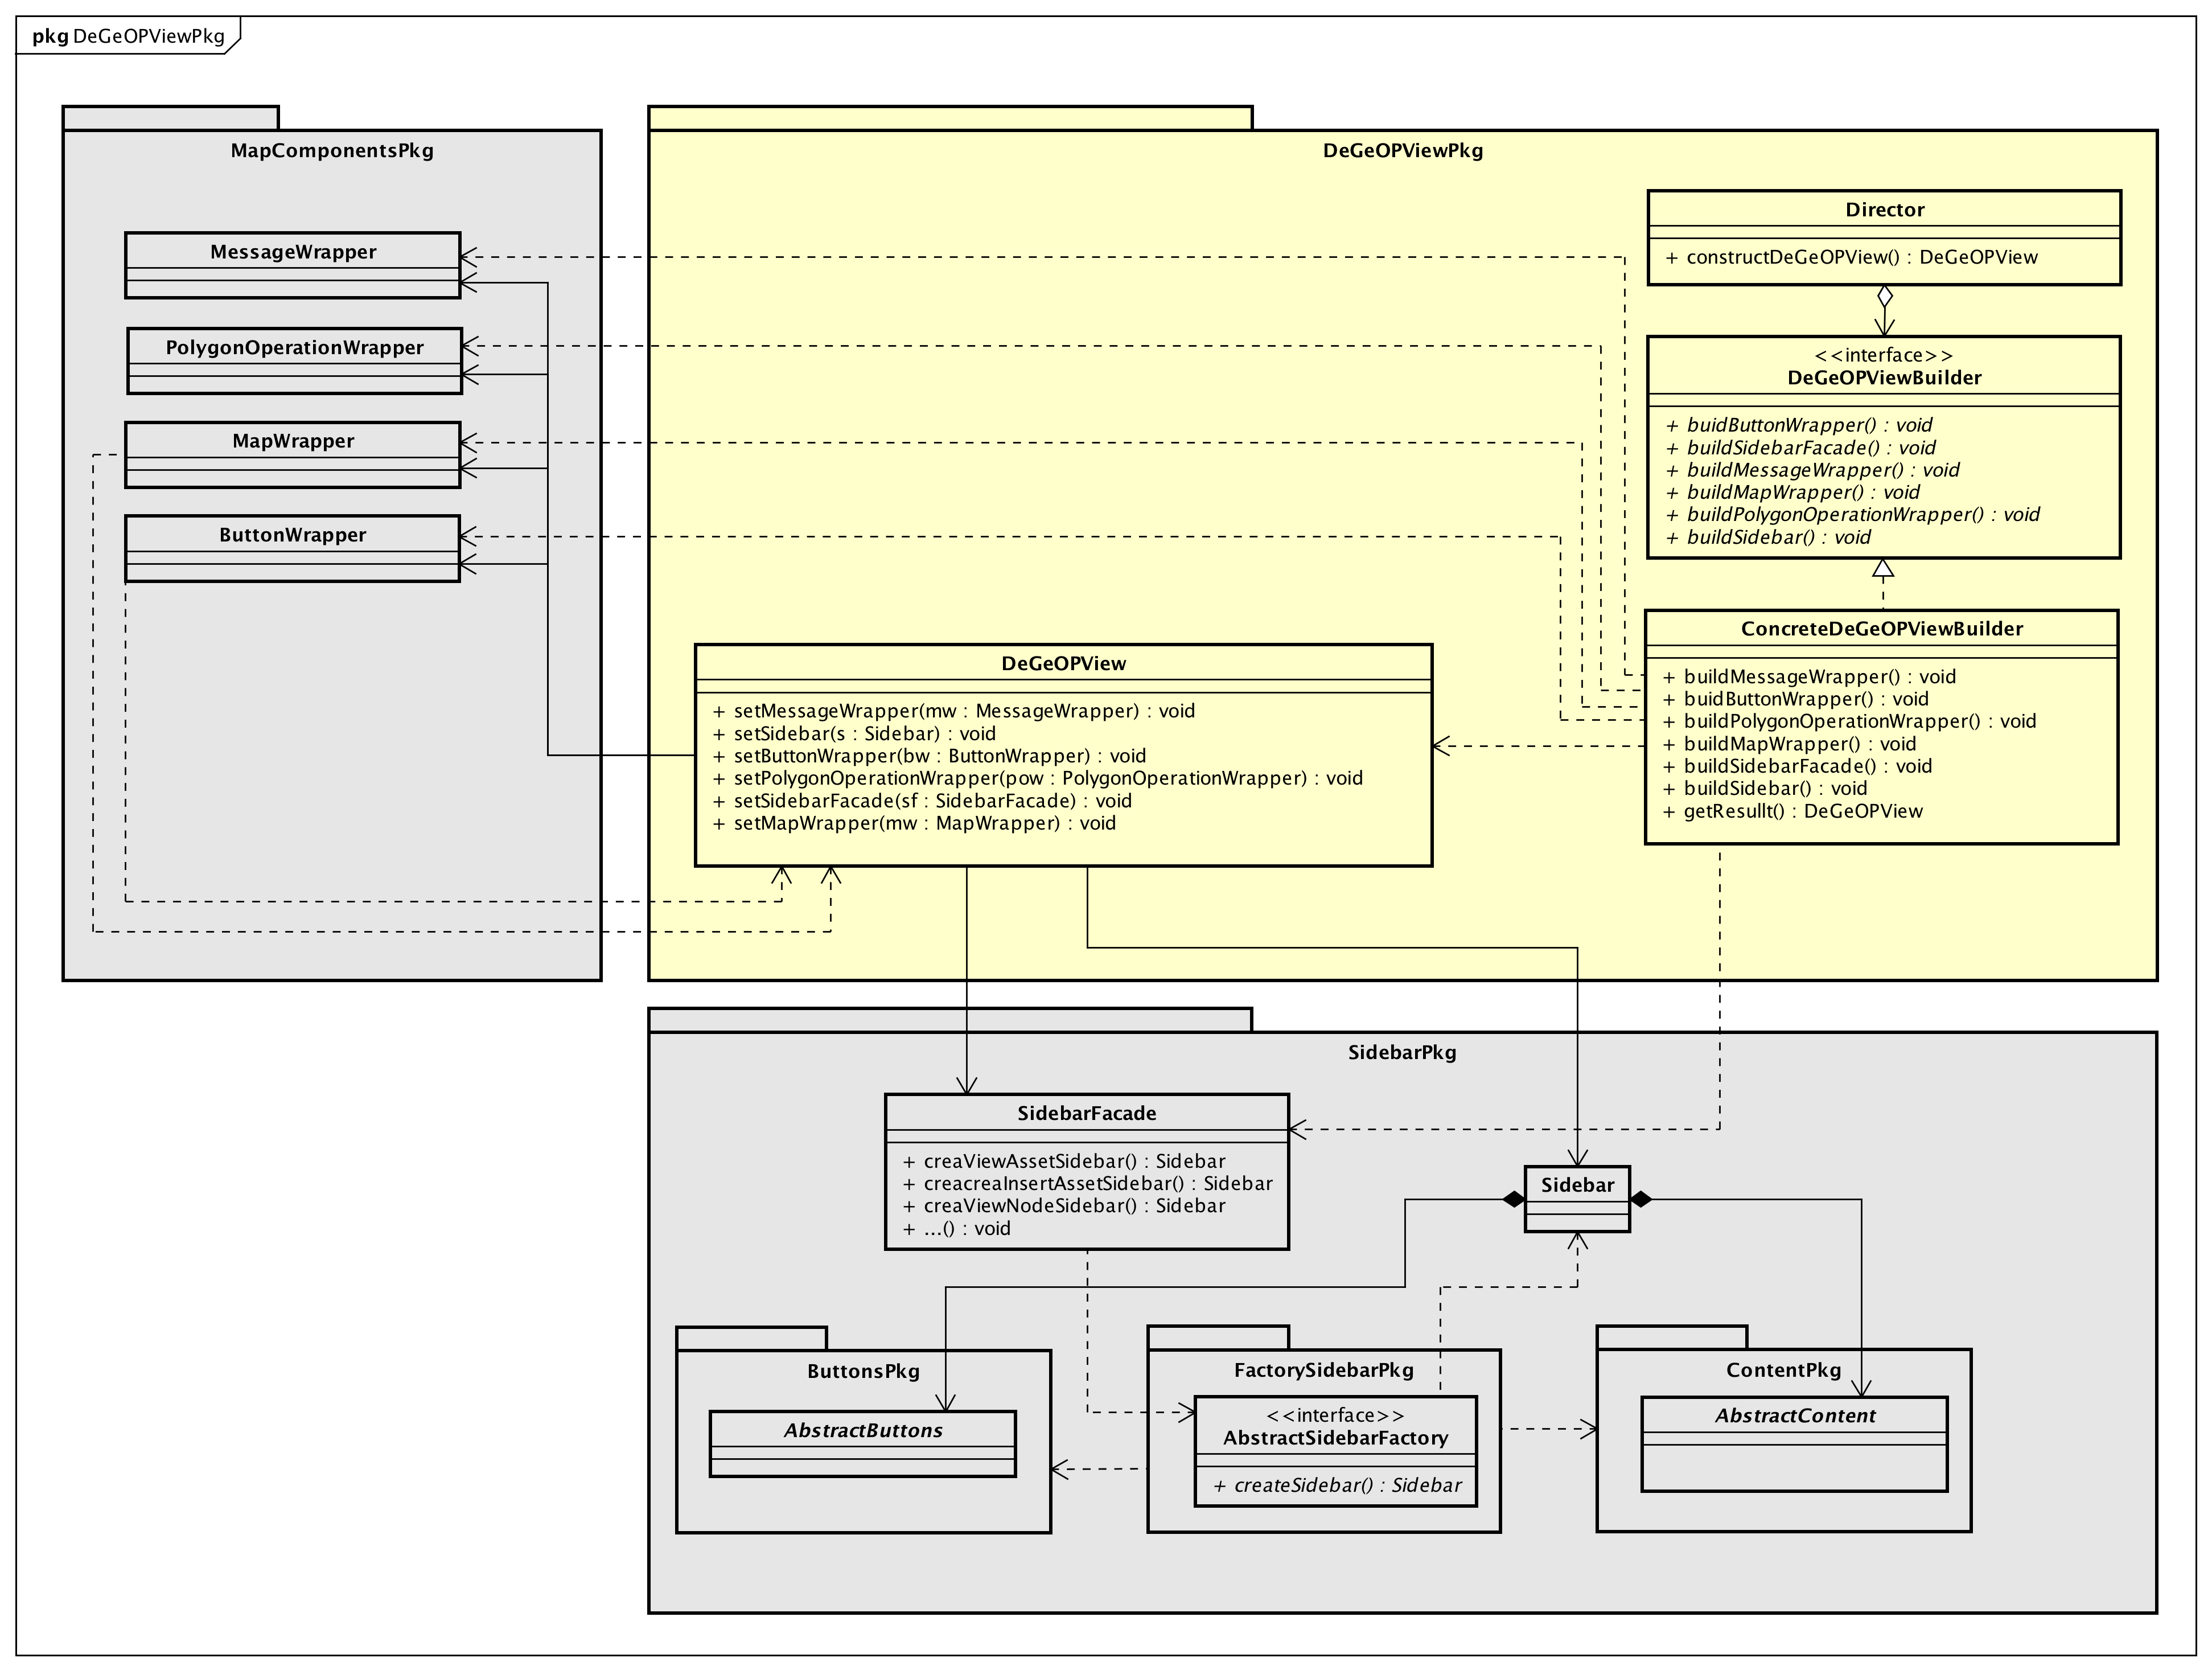
\includegraphics[width=\textwidth]{img/PkgDiagram/DeGeOPViewPkg.png}
	\caption{Schema componente DeGeOP::ViewPkg::DeGeOPViewPkg}
\end{figure}
\subsubsection{Informazioni sul package}
\begin{itemize}
	\item \textbf{descrizione:} racchiude la \glo{Componente}{componente} principale della view;
	\item \textbf{padre:} \hyperref[pkg::ViewPkg]{ViewPkg};
	\item \textbf{interazioni con altri package:} 
	\begin{itemize}
		\item IN MapComponentsPkg: utilizzo di componenti grafiche;
		\item OUT MapComponentsPkg: utilizzo di componenti grafiche;
		\item OUT SidebarPkg: utilizzo della sidebar.
	\end{itemize}
	\item \textbf{classi contenute:}
	\begin{itemize}
		\item ConcreteDeGeOPViewBuilder;
		\item DeGeOPView;
		\item DeGeOPViewBuilder;
		\item Director.
	\end{itemize}
\end{itemize}
\subsubsection{Classi}
\paragraph{ConcreteDeGeOPViewBuilder}
\begin{itemize}
	\item \textbf{descrizione:} rappresenta un'implementazione di DeGeOPViewBuilder;
	\item \textbf{utilizzo:} i suoi metodi vengono invocati dal director per creare le varie componenti di DeGeOPView;
	\item \textbf{relazioni con altre classi:} 
	\begin{itemize}
		\item OUT ButtonWrapper;
		\item OUT DeGeOPView;
		\item OUT MapWrapper;
		\item OUT MessageWrapper;
		\item OUT PolygonOperationWrapper;
		\item OUT SidebarFacade.
	\end{itemize}
\end{itemize}
\paragraph{DeGeOPView}
\begin{itemize}
	\item \textbf{descrizione:} rappresenta l'oggetto grafico radice, che comprende l'intera View del prodotto;
	\item \textbf{utilizzo:} i suoi metodi setter sono richiamati da ConcreteDeGeOPViewBuilder per impostare i suoi campi dati. La classe effettua il subscribe sullo Store per ricevere gli aggiornamenti ;
	\item \textbf{relazioni con altre classi:} 
	\begin{itemize}
		\item IN ButtonWrapper;
		\item IN ConcreteDeGeOPViewBuilder;
		\item IN MapWrapper;
		\item OUT ButtonWrapper;
		\item OUT MapWrapper;
		\item OUT MessageWrapper;
		\item OUT PolygonOperationWrapper;
		\item OUT Sidebar;
		\item OUT SidebarFacade;
		\item OUT StoreDeGeOP.
	\end{itemize}
\end{itemize}
\paragraph{DeGeOPViewBuilder}
\begin{itemize}
	\item \textbf{descrizione:} interfaccia che rappresenta un builder per l'oggetto DeGeOPView;
	\item \textbf{utilizzo:} viene implementata per istanziare un builder concreto di DeGeOPView;
	\item \textbf{relazioni con altre classi:} 
	\begin{itemize}
		\item IN Director.
	\end{itemize}
\end{itemize}
\paragraph{Director}
\begin{itemize}
	\item \textbf{descrizione:} rappresenta il director del \glo{Design pattern}{design pattern} builder usato per creare la View;
	\item \textbf{utilizzo:} è utilizzato per avviare la costruzione di DeGeOPView chiamando i metodi di un DeGeOPViewBuilder;
	\item \textbf{relazioni con altre classi:} 
	\begin{itemize}
		\item OUT DeGeOPViewBuilder.
	\end{itemize}
\end{itemize}
\newpage
\subsection{DeGeOP::ViewPkg::MapComponentsPkg}
\label{pkg::MapComponentsPkg}
\begin{figure}[H]
	\centering
	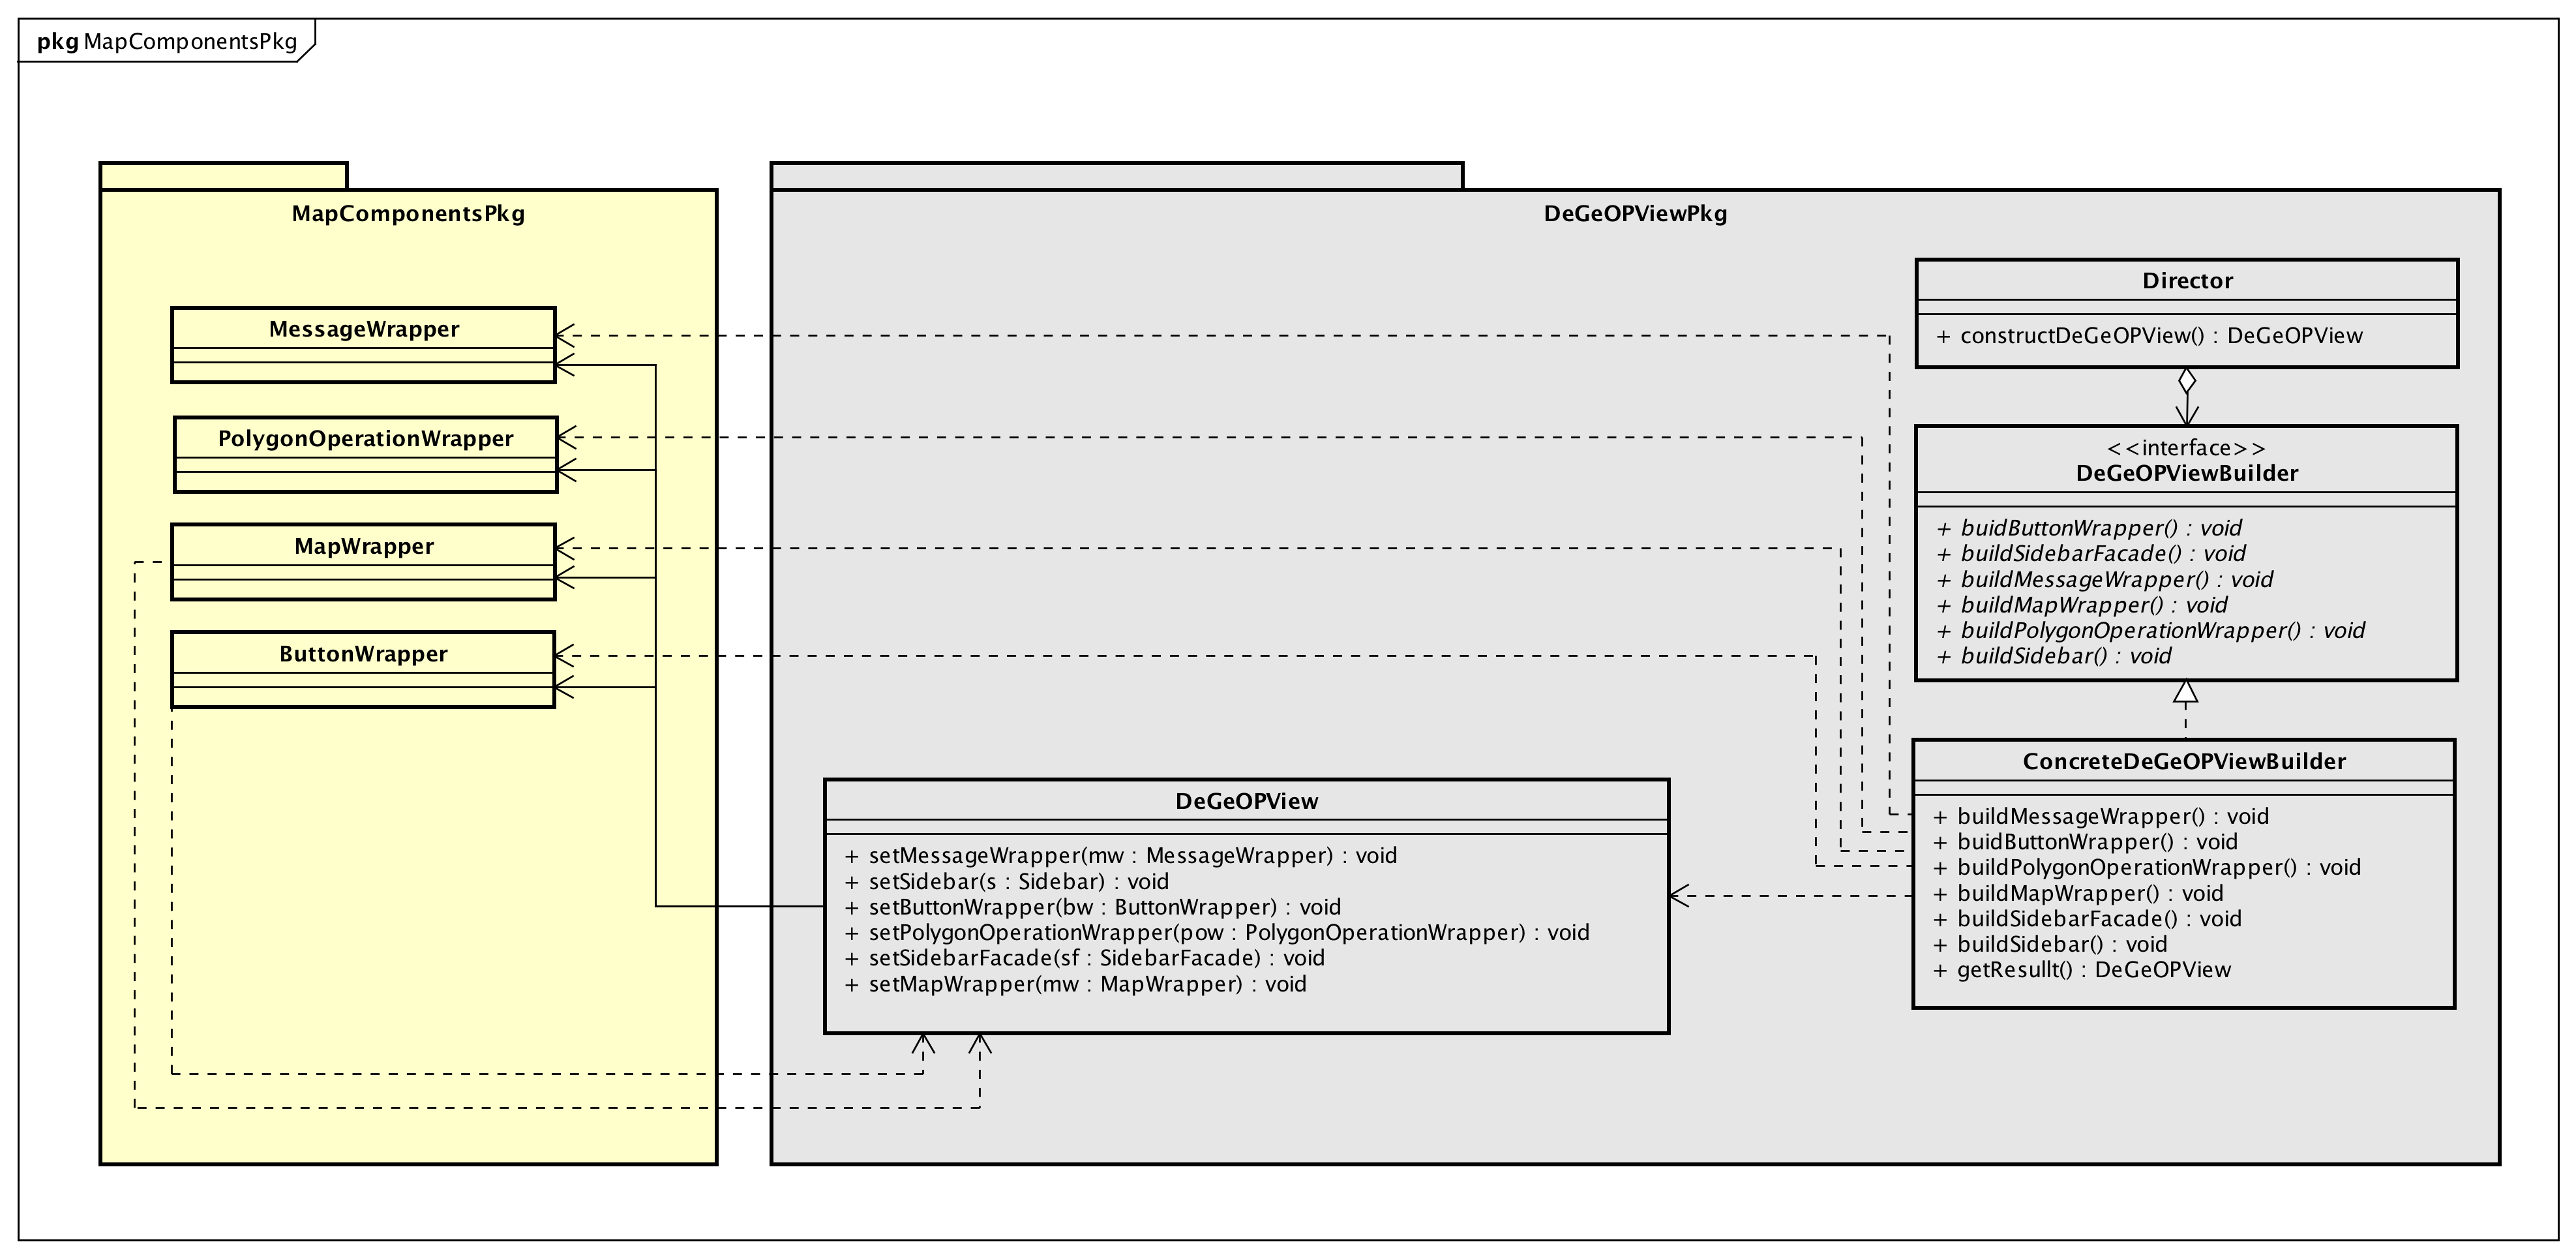
\includegraphics[width=\textwidth]{img/PkgDiagram/MapComponentsPkg.png}
	\caption{Schema componente DeGeOP::ViewPkg::MapComponentsPkg}
\end{figure}
\subsubsection{Informazioni sul package}
\begin{itemize}
	\item \textbf{descrizione:} racchiude le componenti relative alla mappa e ai pulsanti sopra di essa;
	\item \textbf{padre:} \hyperref[pkg::ViewPkg]{ViewPkg};
	\item \textbf{interazioni con altri package:} 
	\begin{itemize}
		\item IN DeGeOPViewPkg: utilizzo di componenti grafiche;
		\item OUT DeGeOPViewPkg: utilizzo di componenti grafiche;
		\item OUT Openlayers: gestione mappa.
	\end{itemize}
	\item \textbf{classi contenute:}
	\begin{itemize}
		\item ButtonWrapper;
		\item MapWrapper;
		\item MessageWrapper;
		\item PolygonOperationWrapper.
	\end{itemize}
	Il package presenta una dipendenza circolare con MapComponentsPkg. Tuttavia tale dipendenza viene risolta tramite l'utilizzo di un builder che inizializza l'oggetto DeGeOPView costruendo le sue parti. Inoltre, un verso della dipendenza è una dipendenza lasca, quindi non sono stati rilevati problemi da tale dipendenza circolare.
\end{itemize}
\subsubsection{Classi}
\paragraph{ButtonWrapper}
\begin{itemize}
	\item \textbf{descrizione:} rappresenta una classe wrapper per visualizzare una serie di bottoni con cui è possibile eseguire varie operazioni;
	\item \textbf{utilizzo:} viene utilizzato per mostrare sulla mappa una serie di bottoni;
	\item \textbf{relazioni con altre classi:} 
	\begin{itemize}
		\item IN ConcreteDeGeOPViewBuilder;
		\item IN DeGeOPView;
		\item OUT DeGeOPView.
	\end{itemize}
\end{itemize}
\paragraph{MapWrapper}
\begin{itemize}
	\item \textbf{descrizione:} rappresenta una classe wrapper per visualizzare la mappa;
	\item \textbf{utilizzo:} viene utilizzata per visualizzare una mappa e permettere all'utente di interagire con essa;
	\item \textbf{relazioni con altre classi:} 
	\begin{itemize}
		\item IN ConcreteDeGeOPViewBuilder;
		\item IN DeGeOPView;
		\item OUT DeGeOPView.
	\end{itemize}
\end{itemize}
\paragraph{MessageWrapper}
\begin{itemize}
	\item \textbf{descrizione:} rappresenta una classe wrapper per visualizzare un messaggio;
	\item \textbf{utilizzo:} viene utilizzato per mostrare messaggi di errore o di successo sulla mappa;
	\item \textbf{relazioni con altre classi:} 
	\begin{itemize}
		\item IN ConcreteDeGeOPViewBuilder;
		\item IN DeGeOPView.
	\end{itemize}
\end{itemize}
\paragraph{PolygonOperationWrapper}
\begin{itemize}
	\item \textbf{descrizione:} rappresenta una classe wrapper per visualizzare un bottone con cui è possibile effettuare operazioni sul perimetro di un poligono sulla mappa;
	\item \textbf{utilizzo:} invocando i suoi metodi è possibile iniziare a disegnare il poligono su mappa oppure cancellare l'ultimo segmento disegnato;
	\item \textbf{relazioni con altre classi:} 
	\begin{itemize}
		\item IN ConcreteDeGeOPViewBuilder;
		\item IN DeGeOPView.
	\end{itemize}
\end{itemize}
\newpage
\subsection{DeGeOP::ViewPkg::SidebarPkg}
\label{pkg::SidebarPkg}
\begin{figure}[H]
	\centering
	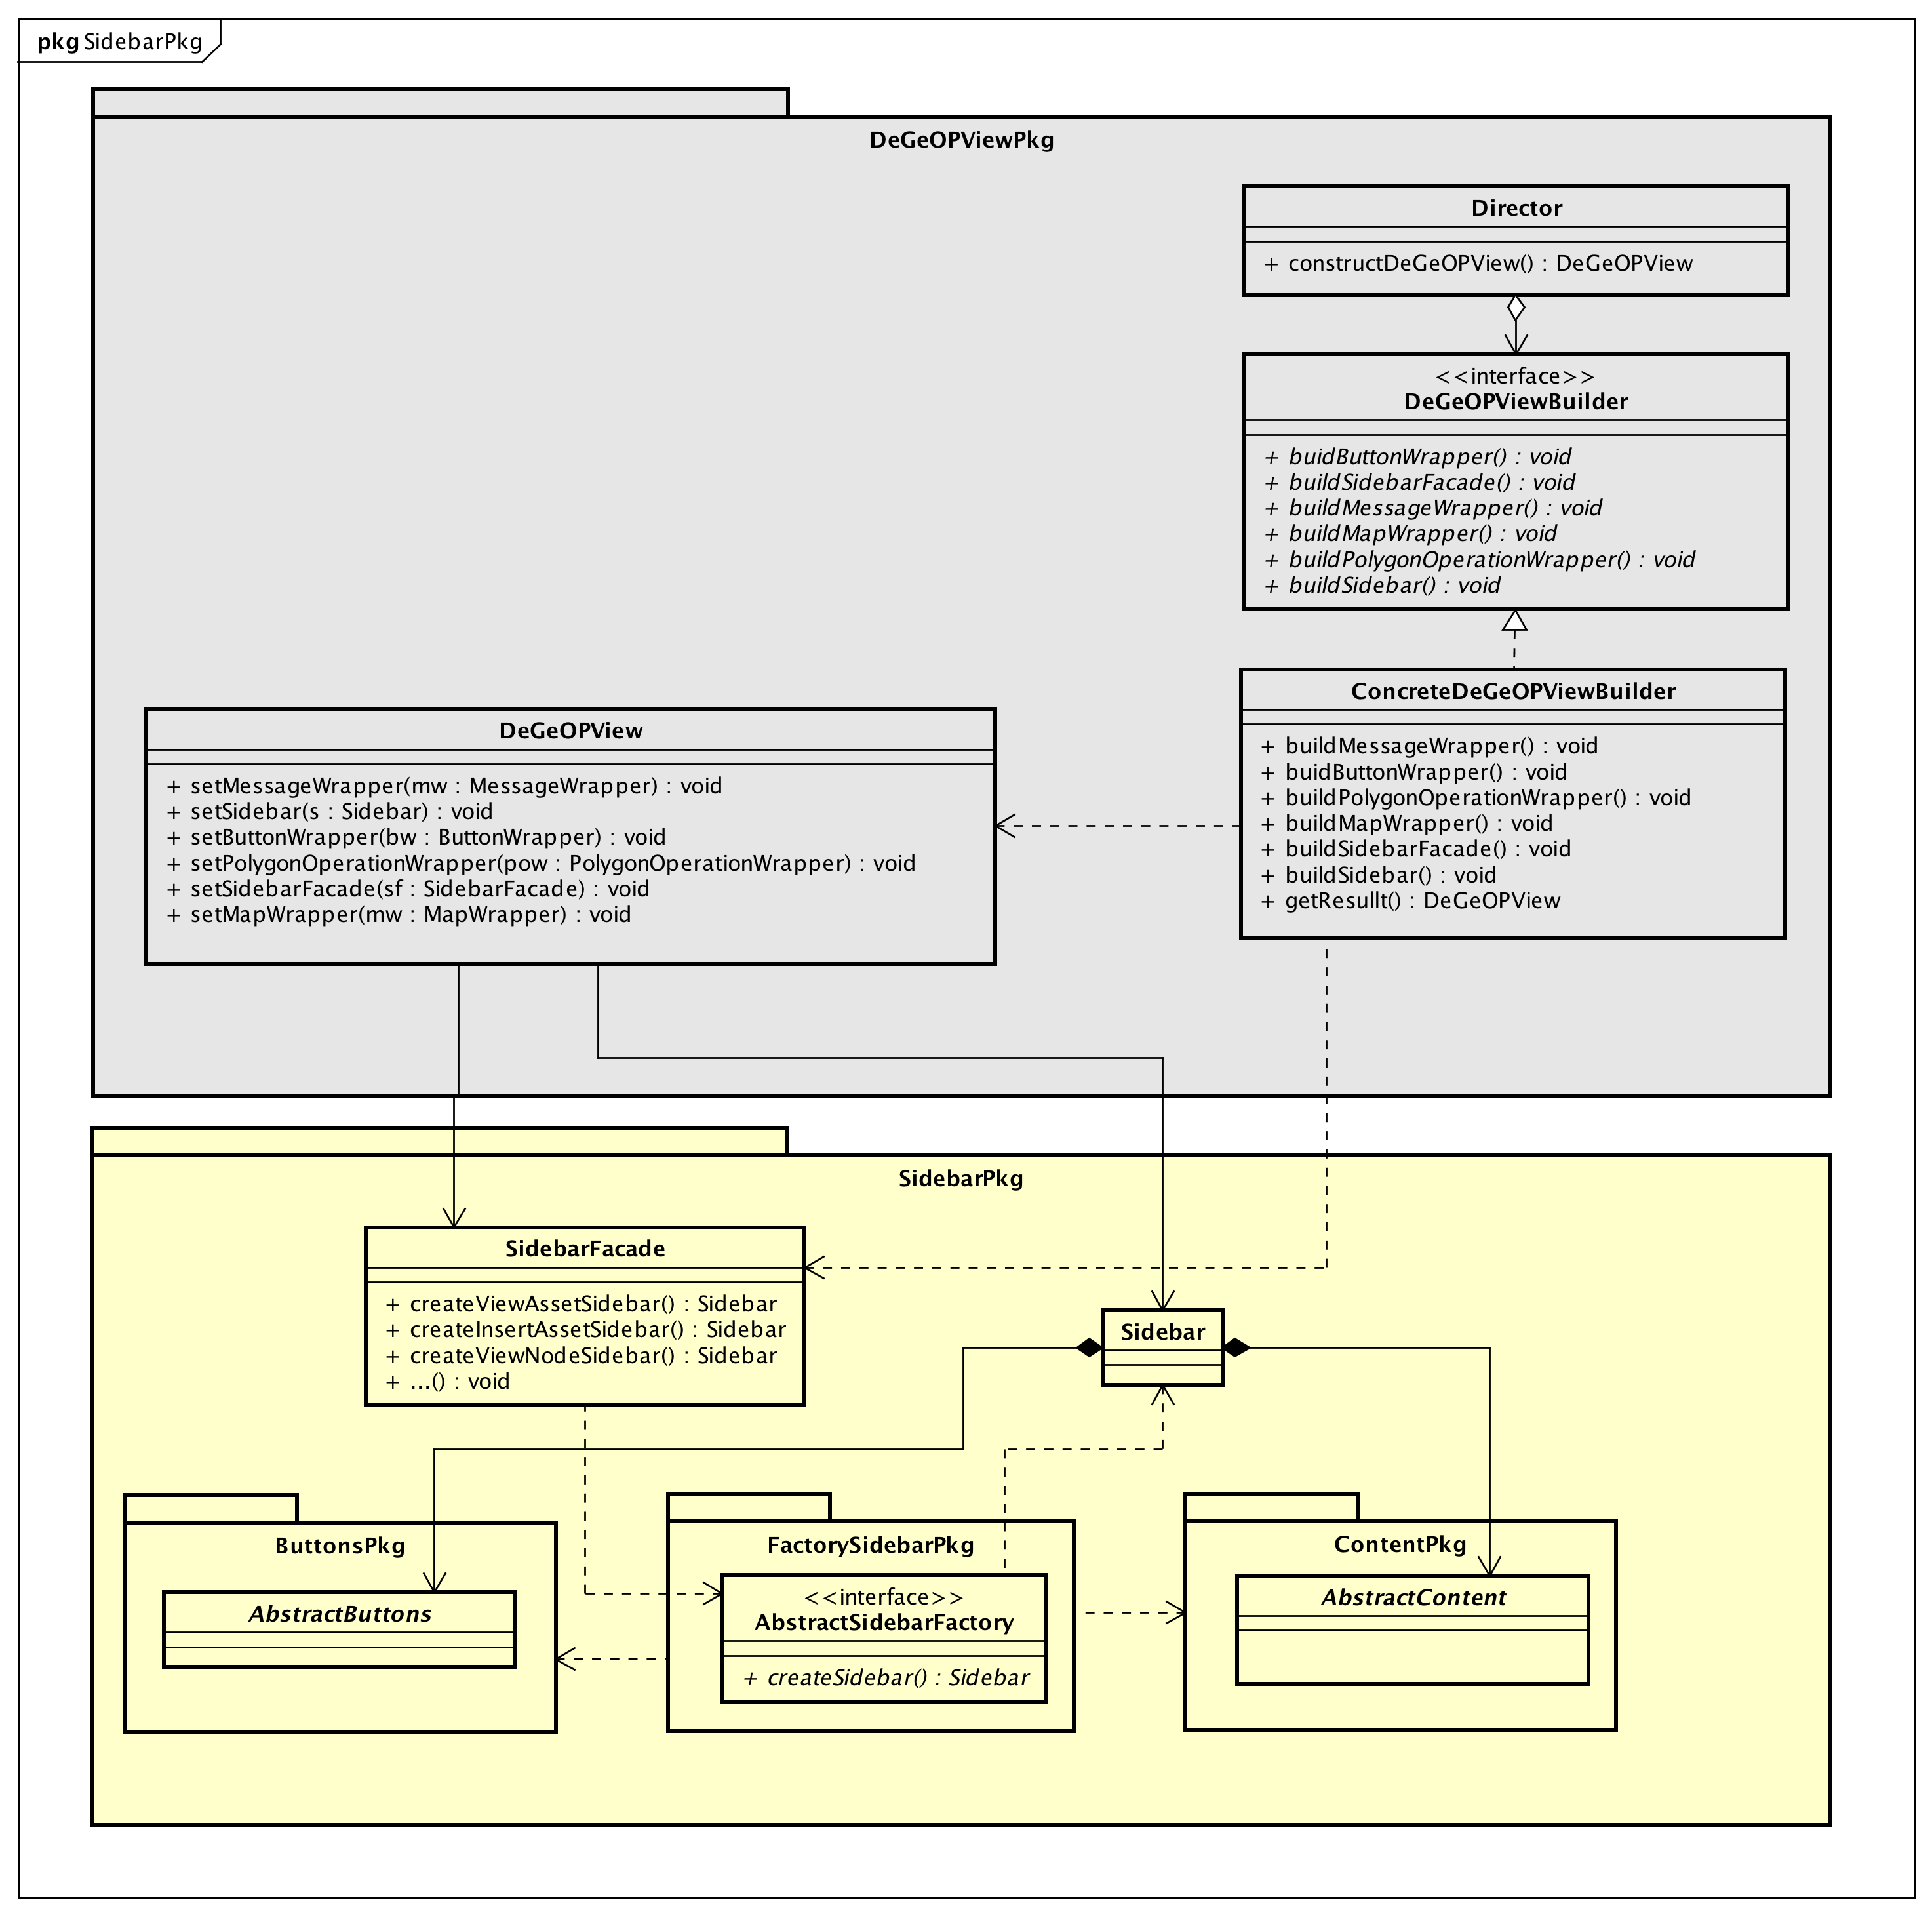
\includegraphics[width=\textwidth]{img/PkgDiagram/SidebarPkg.png}
	\caption{Schema componente DeGeOP::ViewPkg::SidebarPkg}
\end{figure}
\subsubsection{Informazioni sul package}
\begin{itemize}
	\item \textbf{descrizione:} racchiude le componenti necessarie alla rappresentazione della sidebar;
	\item \textbf{padre:} \hyperref[pkg::ViewPkg]{ViewPkg};
	\item \textbf{package contenuti:}
	\begin{itemize}
		\item SidebarPkg::\hyperref[pkg::ButtonsPkg]{ButtonsPkg};
		\item SidebarPkg::\hyperref[pkg::ContentPkg]{ContentPkg};
		\item SidebarPkg::\hyperref[pkg::FactorySidebarPkg]{FactorySidebarPkg}.
	\end{itemize}
	\item \textbf{interazioni con altri package:} 
	\begin{itemize}
		\item IN DeGeOPViewPkg: utilizzo della sidebar.
	\end{itemize}
	\item \textbf{classi contenute:}
	\begin{itemize}
		\item Sidebar;
		\item SidebarFacade.
	\end{itemize}
\end{itemize}
\subsubsection{Classi}
\paragraph{Sidebar}
\begin{itemize}
	\item \textbf{descrizione:} rappresenta una sidebar contenente una serie di componenti grafiche;
	\item \textbf{utilizzo:} renderizza una sidebar composta da contenuto in cui l'utente può compilare i dati e da bottoni che permettono di eseguire varie operazioni, come ad esempio inserimenti e modifiche;
	\item \textbf{relazioni con altre classi:} 
	\begin{itemize}
		\item IN DeGeOPView;
		\item OUT AbstractButtons;
		\item OUT AbstractContent.
	\end{itemize}
\end{itemize}
\paragraph{SidebarFacade}
\begin{itemize}
	\item \textbf{descrizione:} rappresenta un Facade tra DeGeOPView e Abstract;
	\item \textbf{utilizzo:} i suoi metodi vengono invocati per la creazione di Sidebar di vari tipologie senza che DeGeOPView necessiti di conoscere del tipo concreto delle Factory. Facade utilizza SidebarFactory concrete all'interno dei suoi metodi;
	\item \textbf{relazioni con altre classi:} 
	\begin{itemize}
		\item IN ConcreteDeGeOPViewBuilder;
		\item IN DeGeOPView;
		\item OUT AnalysisSidebarFactory;
		\item OUT EditAssetSidebarFactory;
		\item OUT EditEdgeSidebarFactory;
		\item OUT EditNodeSidebarFactory;
		\item OUT EditScenarioSidebarFactory;
		\item OUT InsertAssetSidebarFactory;
		\item OUT InsertEdgeSidebarFactory;
		\item OUT InsertNodeSidebarFactory;
		\item OUT InsertScenarioSidebarFactory;
		\item OUT ViewAssetSidebarFactory;
		\item OUT ViewEdgeSidebarFactory;
		\item OUT ViewNodeSidebarFactory;
		\item OUT ViewScenarioSidebarFactory.
	\end{itemize}
\end{itemize}
\newpage
\subsection{DeGeOP::ViewPkg::SidebarPkg::FactorySidebarPkg}
\label{pkg::FactorySidebarPkg}
\begin{figure}[H]
	\centering
	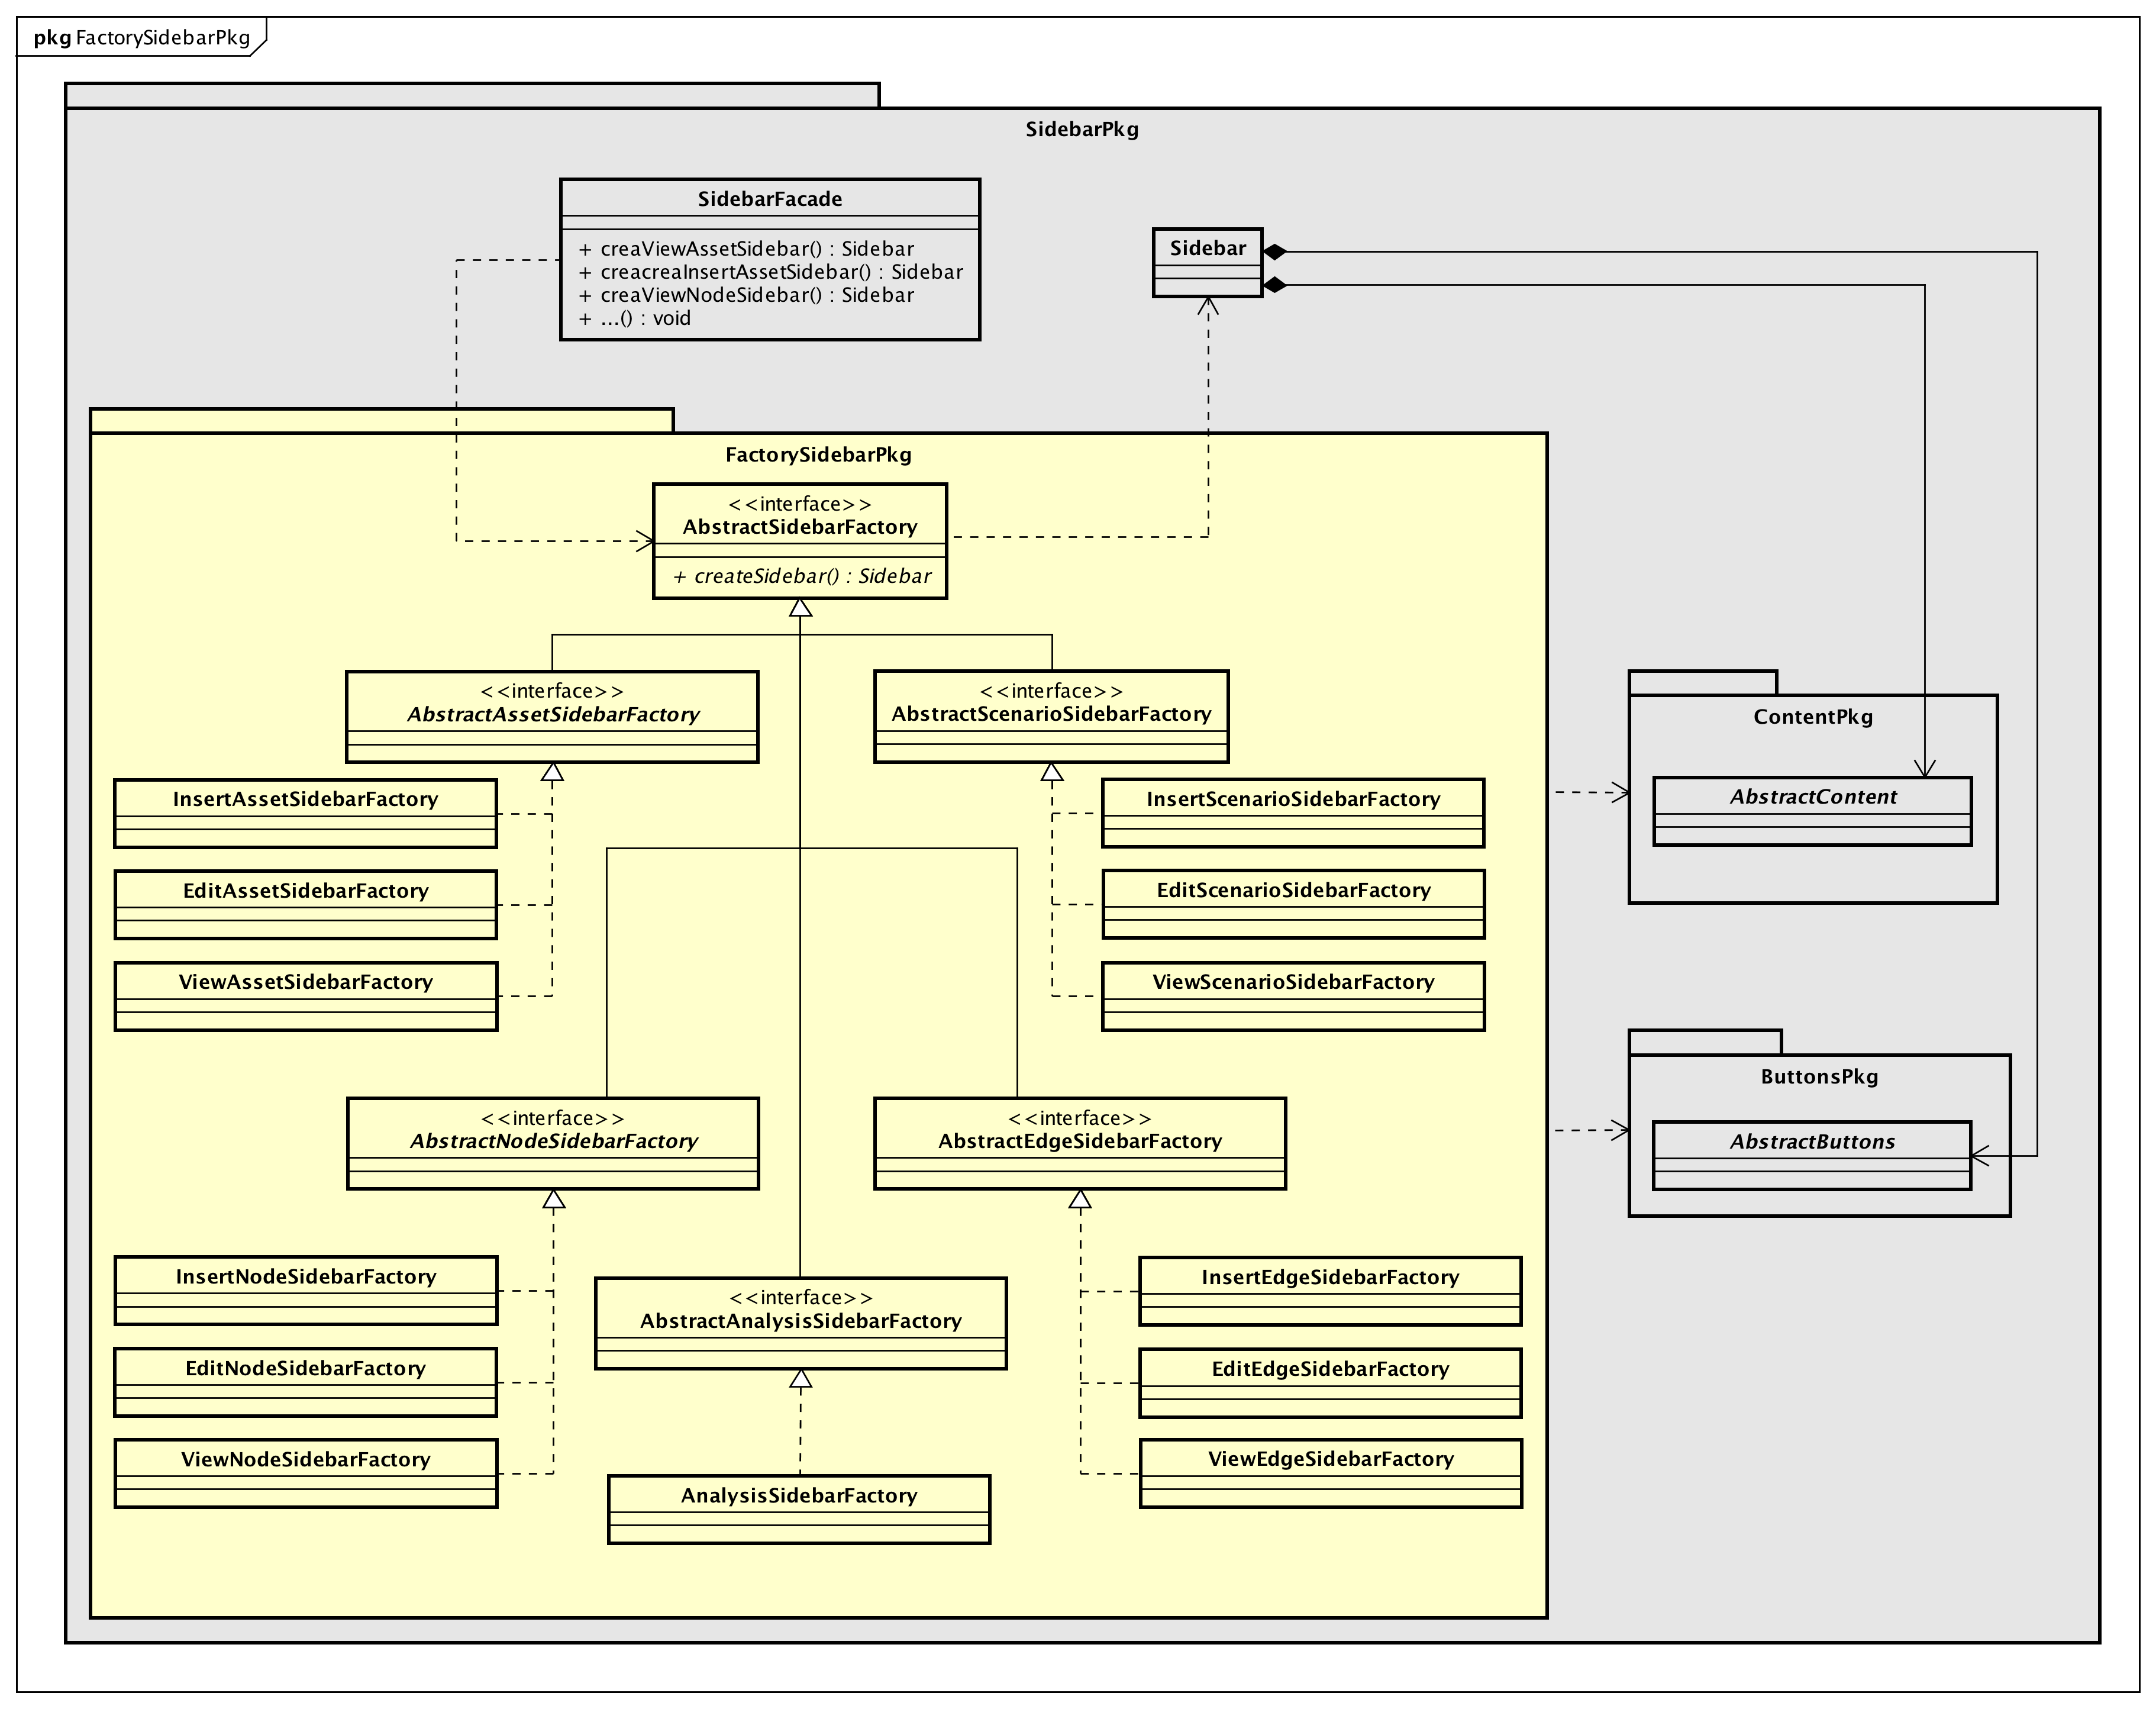
\includegraphics[width=\textwidth]{img/PkgDiagram/FactorySidebarPkg.png}
	\caption{Schema componente DeGeOP::ViewPkg::SidebarPkg::FactorySidebarPkg}
\end{figure}
\subsubsection{Informazioni sul package}
\begin{itemize}
	\item \textbf{descrizione:} Racchiude le componenti Factory per la sidebar;
	\item \textbf{padre:} \hyperref[pkg::SidebarPkg]{SidebarPkg};
	\item \textbf{interazioni con altri package:} 
	\begin{itemize}
		\item OUT ContentPkg: creazione contenuto della sidebar.
	\end{itemize}
	\item \textbf{classi contenute:}
	\begin{itemize}
		\item AbstractAnalysisSidebarFactory;
		\item AbstractAssetSidebarFactory;
		\item AbstractEdgeSidebarFactory;
		\item AbstractNodeSidebarFactory;
		\item AbstractScenarioSidebarFactory;
		\item AbstractSidebarFactory;
		\item AnalysisSidebarFactory;
		\item EditAssetSidebarFactory;
		\item EditEdgeSidebarFactory;
		\item EditNodeSidebarFactory;
		\item EditScenarioSidebarFactory;
		\item InsertAssetSidebarFactory;
		\item InsertEdgeSidebarFactory;
		\item InsertNodeSidebarFactory;
		\item InsertScenarioSidebarFactory;
		\item ViewAssetSidebarFactory;
		\item ViewEdgeSidebarFactory;
		\item ViewNodeSidebarFactory;
		\item ViewScenarioSidebarFactory.
	\end{itemize}
\end{itemize}
\subsubsection{Classi}
\paragraph{AbstractAnalysisSidebarFactory}
\begin{itemize}
	\item \textbf{descrizione:} abstract factory relativa alla sidebar analisi di danno;
	\item \textbf{utilizzo:} viene usata come interfaccia di specializzazione fra abstractSidebar e le istanze di sidebar specifiche.
\end{itemize}
\paragraph{AbstractAssetSidebarFactory}
\begin{itemize}
	\item \textbf{descrizione:} abstract factory relativa alla sidebar asset;
	\item \textbf{utilizzo:}  viene usata come interfaccia di specializzazione fra abstractSidebar e le istanze di sidebar specifiche.
\end{itemize}
\paragraph{AbstractEdgeSidebarFactory}
\begin{itemize}
	\item \textbf{descrizione:} abstract factory relativa alla sidebar archi;
	\item \textbf{utilizzo:} viene usata come interfaccia di specializzazione fra abstractSidebar e le istanze di sidebar specifiche.
\end{itemize}
\paragraph{AbstractNodeSidebarFactory}
\begin{itemize}
	\item \textbf{descrizione:} abstract factory relativa alla sidebar nodi;
	\item \textbf{utilizzo:} viene usata come interfaccia di specializzazione fra abstractSidebar e le istanze di sidebar specifiche.
\end{itemize}
\paragraph{AbstractScenarioSidebarFactory}
\begin{itemize}
	\item \textbf{descrizione:} abstract factory relativa alla sidebar scenari;
	\item \textbf{utilizzo:} viene usata come interfaccia di specializzazione fra abstractSidebar e le istanze di sidebar specifiche.
\end{itemize}
\paragraph{AbstractSidebarFactory}
\begin{itemize}
	\item \textbf{descrizione:} una classe d'interfaccia rappresentante una sidebar con il relativo contenuto;
	\item \textbf{utilizzo:} è utilizzata da SidebarFacade per la creazione di Sidebar.
\end{itemize}
\paragraph{AnalysisSidebarFactory}
\begin{itemize}
	\item \textbf{descrizione:} rappresenta una factory concreta di una sidebar relativa alle analisi di danno;
	\item \textbf{utilizzo:} viene utilizzata da SidebarFacade per la creazione di Sidebar relativa alle analisi di danno;
	\item \textbf{relazioni con altre classi:} 
	\begin{itemize}
		\item IN SidebarFacade;
		\item OUT AnalysisButtons;
		\item OUT AnalysisContent.
	\end{itemize}
\end{itemize}
\paragraph{EditAssetSidebarFactory}
\begin{itemize}
	\item \textbf{descrizione:} rappresenta una factory concreta di una sidebar relativa alla modifica di un asset;
	\item \textbf{utilizzo:} viene utilizzata da SidebarFacade per la creazione di Sidebar per la modifica di un asset;
	\item \textbf{relazioni con altre classi:} 
	\begin{itemize}
		\item IN SidebarFacade;
		\item OUT EditAssetButtons;
		\item OUT EditAssetContent.
	\end{itemize}
\end{itemize}
\paragraph{EditEdgeSidebarFactory}
\begin{itemize}
	\item \textbf{descrizione:} rappresenta una factory concreta di una sidebar relativa alla modifica di un arco;
	\item \textbf{utilizzo:} viene utilizzata da SidebarFacade per la creazione di Sidebar per la modifica di un arco;
	\item \textbf{relazioni con altre classi:} 
	\begin{itemize}
		\item IN SidebarFacade;
		\item OUT EditEdgeButtons;
		\item OUT EditEdgeContent.
	\end{itemize}
\end{itemize}
\paragraph{EditNodeSidebarFactory}
\begin{itemize}
	\item \textbf{descrizione:} rappresenta una factory concreta di una sidebar relativa all'inserimento di un nodo;
	\item \textbf{utilizzo:} viene utilizzata da SidebarFacade per la creazione di Sidebar per l'inserimento di un nodo;
	\item \textbf{relazioni con altre classi:} 
	\begin{itemize}
		\item IN SidebarFacade;
		\item OUT EditNodeButtons;
		\item OUT EditNodeContent.
	\end{itemize}
\end{itemize}
\paragraph{EditScenarioSidebarFactory}
\begin{itemize}
	\item \textbf{descrizione:} rappresenta una factory concreta di una sidebar relativa all'inserimento di uno scenario di danno;
	\item \textbf{utilizzo:} viene utilizzata da SidebarFacade per la creazione di Sidebar per l'inserimento di uno scenario di danno;
	\item \textbf{relazioni con altre classi:} 
	\begin{itemize}
		\item IN SidebarFacade;
		\item OUT EditScenarioButtons;
		\item OUT EditScenarioContent.
	\end{itemize}
\end{itemize}
\paragraph{InsertAssetSidebarFactory}
\begin{itemize}
	\item \textbf{descrizione:} rappresenta una factory concreta di una sidebar relativa all'inserimento di un asset;
	\item \textbf{utilizzo:} viene utilizzata da SidebarFacade per la creazione di Sidebar per l'inserimento di un asset;
	\item \textbf{relazioni con altre classi:} 
	\begin{itemize}
		\item IN SidebarFacade;
		\item OUT InsertAssetButtons;
		\item OUT InsertAssetContent.
	\end{itemize}
\end{itemize}
\paragraph{InsertEdgeSidebarFactory}
\begin{itemize}
	\item \textbf{descrizione:} rappresenta una factory concreta di una sidebar relativa all'inserimento di un arco;
	\item \textbf{utilizzo:} viene utilizzata da SidebarFacade per la creazione di Sidebar per l'inserimento di un arco;
	\item \textbf{relazioni con altre classi:} 
	\begin{itemize}
		\item IN SidebarFacade;
		\item OUT InsertEdgeButtons;
		\item OUT InsertEdgeContent.
	\end{itemize}
\end{itemize}
\paragraph{InsertNodeSidebarFactory}
\begin{itemize}
	\item \textbf{descrizione:} rappresenta una factory concreta di una sidebar relativa all'inserimento di un nodo;
	\item \textbf{utilizzo:} viene utilizzata da SidebarFacade per la creazione di Sidebar per l'inserimento di un nodo;
	\item \textbf{relazioni con altre classi:} 
	\begin{itemize}
		\item IN SidebarFacade;
		\item OUT InsertNodeButtons;
		\item OUT InsertNodeContent.
	\end{itemize}
\end{itemize}
\paragraph{InsertScenarioSidebarFactory}
\begin{itemize}
	\item \textbf{descrizione:} rappresenta una factory concreta di una sidebar relativa all'inserimento di uno scenario di danno;
	\item \textbf{utilizzo:} viene utilizzata da SidebarFacade per la creazione di Sidebar per l'inserimento di uno scenario di danno;
	\item \textbf{relazioni con altre classi:} 
	\begin{itemize}
		\item IN SidebarFacade;
		\item OUT InsertScenarioButtons;
		\item OUT InsertScenarioContent.
	\end{itemize}
\end{itemize}
\paragraph{ViewAssetSidebarFactory}
\begin{itemize}
	\item \textbf{descrizione:} rappresenta una factory concreta di una sidebar relativa alla visualizzazione di un asset;
	\item \textbf{utilizzo:} viene utilizzata da SidebarFacade per la creazione di Sidebar per la visualizzazione di un asset;
	\item \textbf{relazioni con altre classi:} 
	\begin{itemize}
		\item IN SidebarFacade;
		\item OUT ViewAssetButtons;
		\item OUT ViewAssetContent.
	\end{itemize}
\end{itemize}
\paragraph{ViewEdgeSidebarFactory}
\begin{itemize}
	\item \textbf{descrizione:} rappresenta una factory concreta di una sidebar relativa alla visualizzazione di un arco;
	\item \textbf{utilizzo:} viene utilizzata da SidebarFacade per la creazione di Sidebar per la visualizzazione di un arco;
	\item \textbf{relazioni con altre classi:} 
	\begin{itemize}
		\item IN SidebarFacade;
		\item OUT ViewEdgeButtons;
		\item OUT ViewEdgeContent.
	\end{itemize}
\end{itemize}
\paragraph{ViewNodeSidebarFactory}
\begin{itemize}
	\item \textbf{descrizione:} rappresenta una factory concreta di una sidebar relativa all'inserimento di un nodo;
	\item \textbf{utilizzo:} viene utilizzata da SidebarFacade per la creazione di Sidebar per l'inserimento di un nodo;
	\item \textbf{relazioni con altre classi:} 
	\begin{itemize}
		\item IN SidebarFacade;
		\item OUT ViewNodeButtons;
		\item OUT ViewNodeContent.
	\end{itemize}
\end{itemize}
\paragraph{ViewScenarioSidebarFactory}
\begin{itemize}
	\item \textbf{descrizione:} rappresenta una factory concreta di una sidebar relativa all'inserimento di uno scenario di danno;
	\item \textbf{utilizzo:} viene utilizzata da SidebarFacade per la creazione di Sidebar per l'inserimento di uno scenario di danno;
	\item \textbf{relazioni con altre classi:} 
	\begin{itemize}
		\item IN SidebarFacade;
		\item OUT ViewScenarioButtons;
		\item OUT ViewScenarioContent.
	\end{itemize}
\end{itemize}
\newpage
\subsection{DeGeOP::ViewPkg::SidebarPkg::ContentPkg}
\label{pkg::ContentPkg}
\begin{figure}[H]
	\centering
	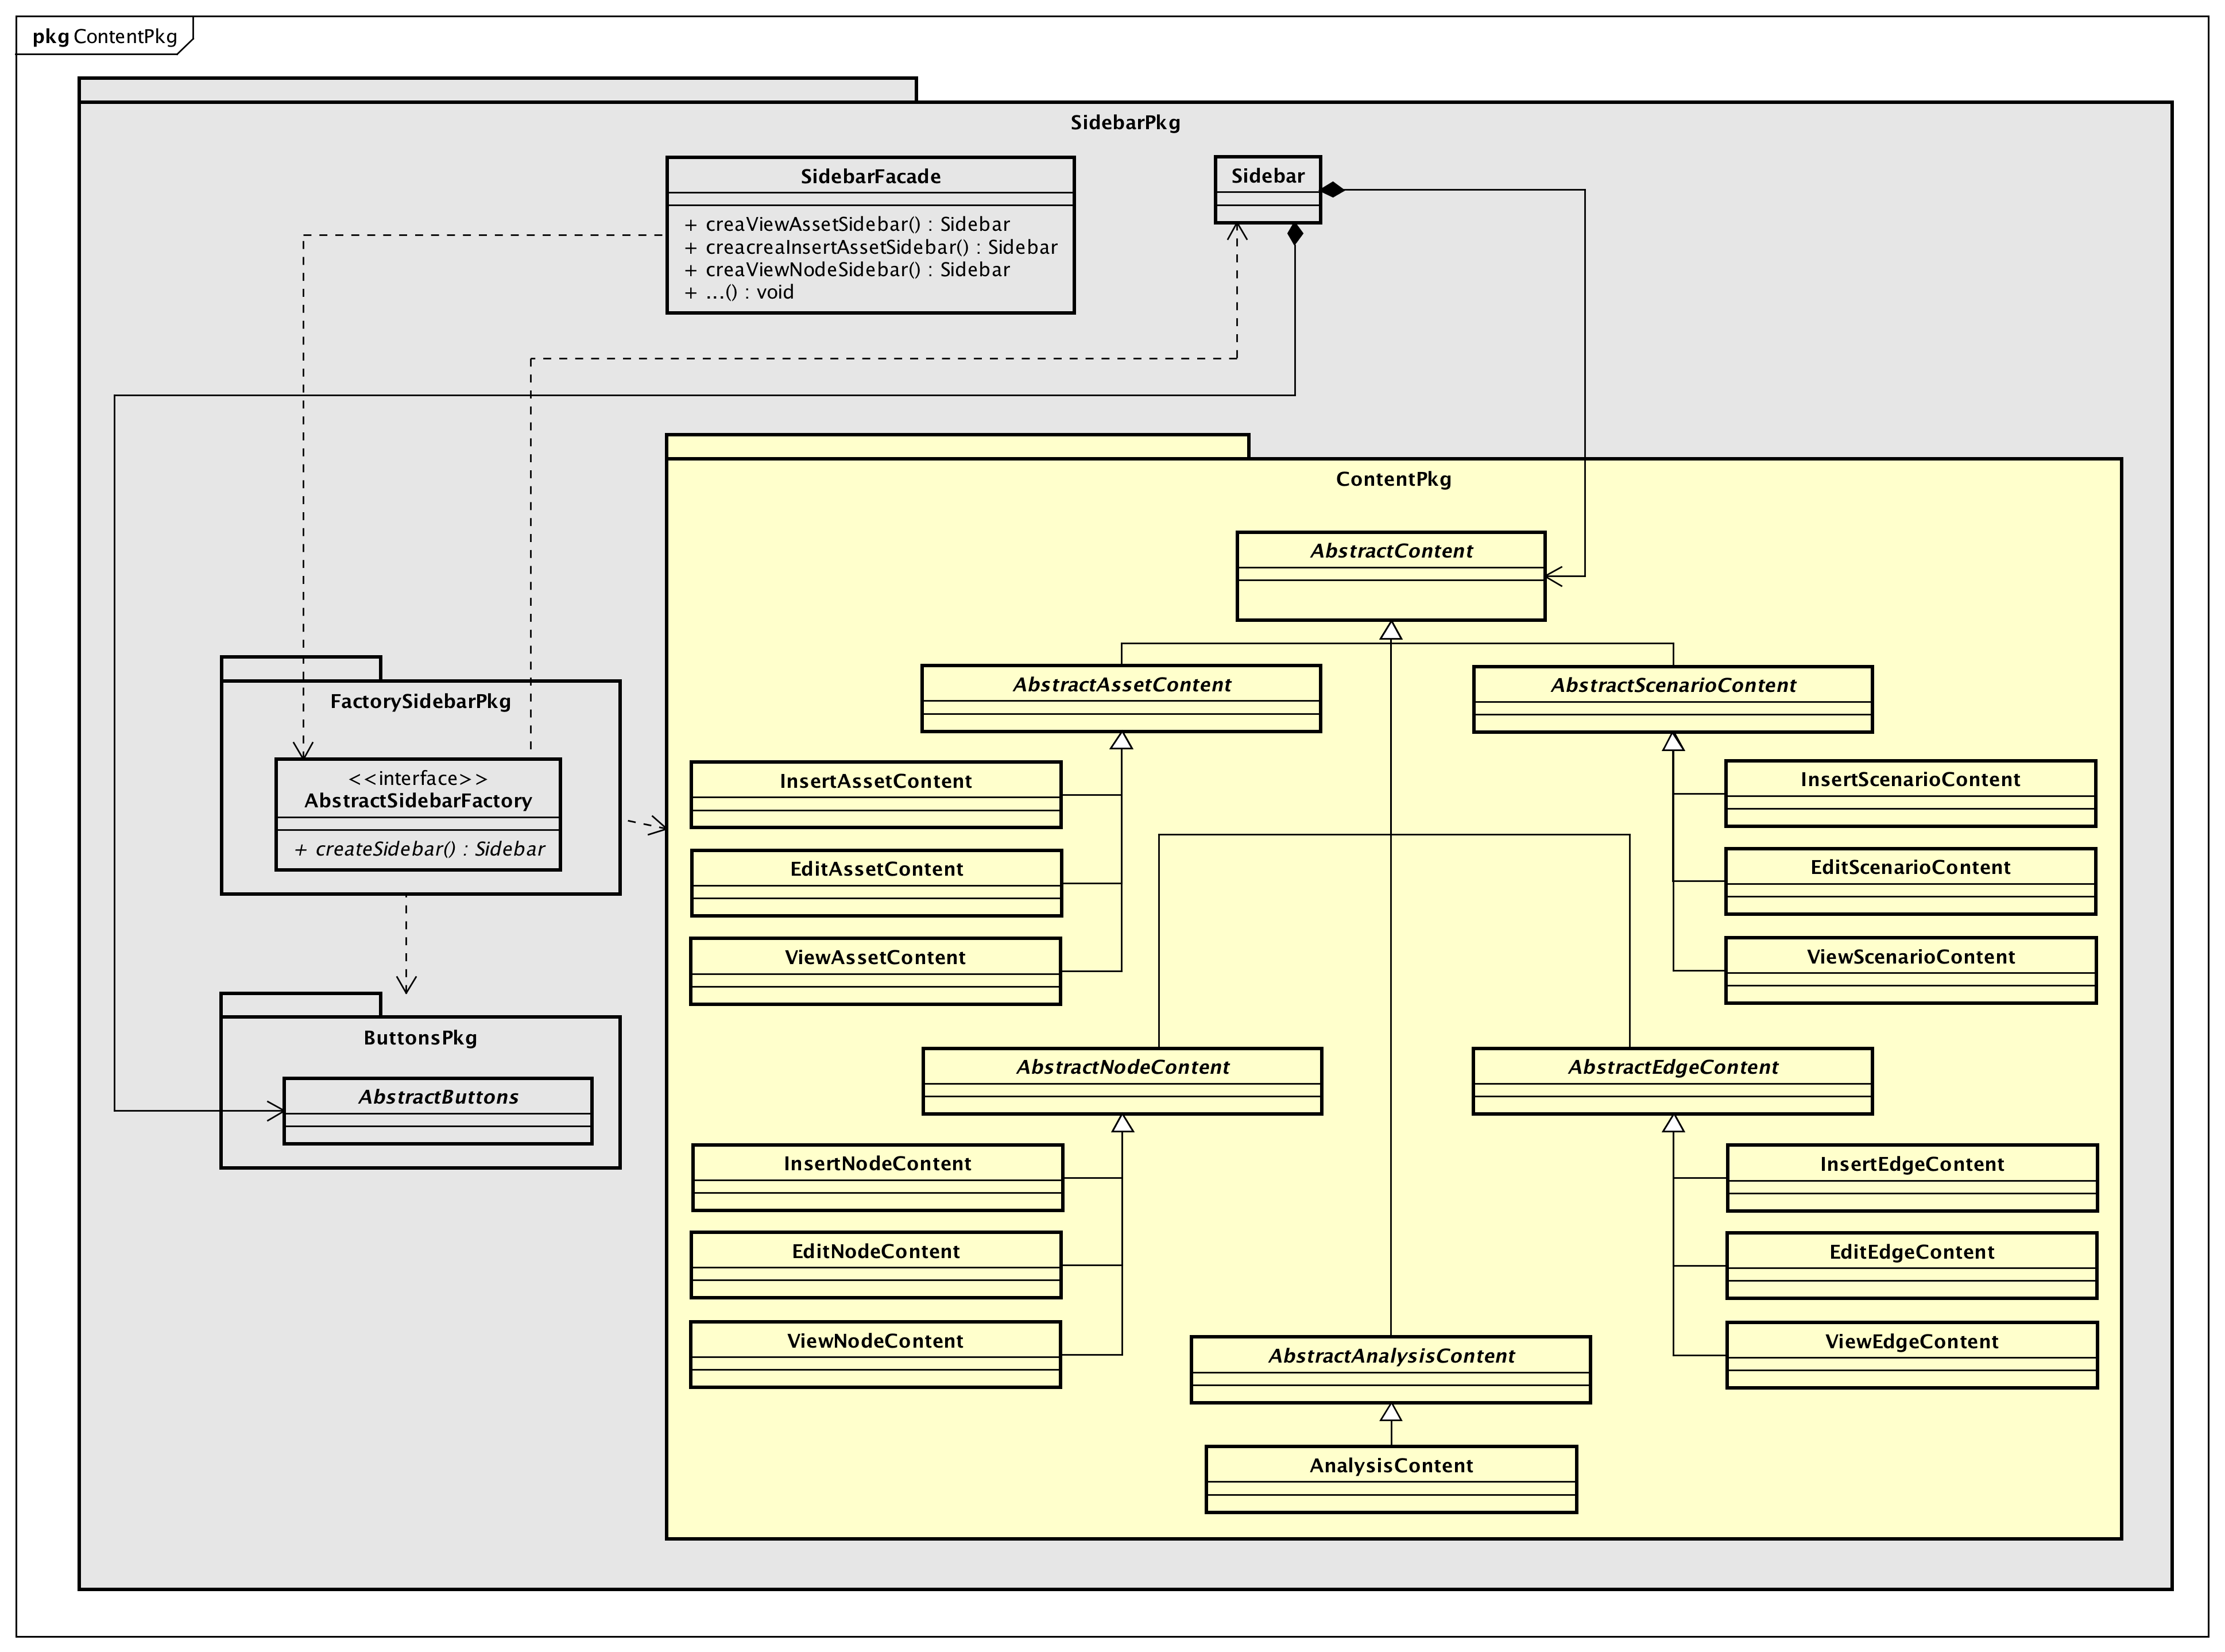
\includegraphics[width=\textwidth]{img/PkgDiagram/ContentPkg.png}
	\caption{Schema componente DeGeOP::ViewPkg::SidebarPkg::ContentPkg}
\end{figure}
\subsubsection{Informazioni sul package}
\begin{itemize}
	\item \textbf{descrizione:} racchiude le componenti che sono relative all'area informativa della Sidebar;
	\item \textbf{padre:} \hyperref[pkg::SidebarPkg]{SidebarPkg};
	\item \textbf{interazioni con altri package:} 
	\begin{itemize}
		\item IN FactorySidebarPkg: creazione contenuto della sidebar;
		\item OUT React-color: visualizzazione palette colori.
	\end{itemize}
	\item \textbf{classi contenute:}
	\begin{itemize}
		\item AbstractAnalysisContent;
		\item AbstractAssetContent;
		\item AbstractContent;
		\item AbstractEdgeContent;
		\item AbstractNodeContent;
		\item AbstractScenarioContent;
		\item AnalysisContent;
		\item EditAssetContent;
		\item EditEdgeContent;
		\item EditNodeContent;
		\item EditScenarioContent;
		\item InsertAssetContent;
		\item InsertEdgeContent;
		\item InsertNodeContent;
		\item InsertScenarioContent;
		\item ViewAssetContent;
		\item ViewEdgeContent;
		\item ViewNodeContent;
		\item ViewScenarioContent.
	\end{itemize}
\end{itemize}
\subsubsection{Classi}
\paragraph{AbstractAnalysisContent}
\begin{itemize}
	\item \textbf{descrizione:} una classe astratta rappresentante il contenuto della sidebar durante le operazioni sulle analisi;
	\item \textbf{utilizzo:} viene usata come interfaccia di specializzazione fra abstractContent e le istanze di contenuti specifiche.
\end{itemize}
\paragraph{AbstractAssetContent}
\begin{itemize}
	\item \textbf{descrizione:} una classe astratta rappresentante il contenuto della sidebar durante le operazioni sugli asset;
	\item \textbf{utilizzo:} viene usata come interfaccia di specializzazione fra abstractContent e le istanze di contenuti specifiche.
\end{itemize}
\paragraph{AbstractContent}
\begin{itemize}
	\item \textbf{descrizione:} una classe d'interfaccia rappresentante il contenuto dell'area informativa nella sidebar;
	\item \textbf{utilizzo:} viene riferita da sidebar in quanto è una delle sue componenti;
	\item \textbf{relazioni con altre classi:} 
	\begin{itemize}
		\item IN Sidebar.
	\end{itemize}
\end{itemize}
\paragraph{AbstractEdgeContent}
\begin{itemize}
	\item \textbf{descrizione:} una classe astratta rappresentante il contenuto della sidebar durante le operazioni sugli archi;
	\item \textbf{utilizzo:} viene usata come interfaccia di specializzazione fra abstractContent e le istanze di contenuti specifiche.
\end{itemize}
\paragraph{AbstractNodeContent}
\begin{itemize}
	\item \textbf{descrizione:} una classe astratta rappresentante il contenuto della sidebar durante le operazioni sui nodi;
	\item \textbf{utilizzo:} viene usata come interfaccia di specializzazione fra abstractContent e le istanze di contenuti specifiche.
\end{itemize}
\paragraph{AbstractScenarioContent}
\begin{itemize}
	\item \textbf{descrizione:} una classe astratta rappresentante il contenuto della sidebar durante le operazioni sugli scenari;
	\item \textbf{utilizzo:} viene usata come interfaccia di specializzazione fra abstractContent e le istanze di contenuti specifiche.
\end{itemize}
\paragraph{AnalysisContent}
\begin{itemize}
	\item \textbf{descrizione:} rappresenta il contenuto della sidebar relativa all'analisi di danno;
	\item \textbf{utilizzo:} viene creata da AnalysisSidebarFactory ;
	\item \textbf{relazioni con altre classi:} 
	\begin{itemize}
		\item IN AnalysisSidebarFactory.
	\end{itemize}
\end{itemize}
\paragraph{EditAssetContent}
\begin{itemize}
	\item \textbf{descrizione:} rappresenta il contenuto della sidebar relativa alla modifica di un asset;
	\item \textbf{utilizzo:} viene creata da EditAssetSidebarFactory ;
	\item \textbf{relazioni con altre classi:} 
	\begin{itemize}
		\item IN EditAssetSidebarFactory.
	\end{itemize}
\end{itemize}
\paragraph{EditEdgeContent}
\begin{itemize}
	\item \textbf{descrizione:} rappresenta il contenuto della sidebar relativa alla modifica di un arco;
	\item \textbf{utilizzo:} viene creata da EditEdgeSidebarFactory ;
	\item \textbf{relazioni con altre classi:} 
	\begin{itemize}
		\item IN EditEdgeSidebarFactory.
	\end{itemize}
\end{itemize}
\paragraph{EditNodeContent}
\begin{itemize}
	\item \textbf{descrizione:} rappresenta il contenuto della sidebar relativa alla modifica di un nodo;
	\item \textbf{utilizzo:} viene creata da EditNodeSidebarFactory ;
	\item \textbf{relazioni con altre classi:} 
	\begin{itemize}
		\item IN EditNodeSidebarFactory.
	\end{itemize}
\end{itemize}
\paragraph{EditScenarioContent}
\begin{itemize}
	\item \textbf{descrizione:} rappresenta il contenuto della Sidebar relativa alla modifica di uno scenario di danno;
	\item \textbf{utilizzo:} viene creata da EditScenarioSidebarFactory ;
	\item \textbf{relazioni con altre classi:} 
	\begin{itemize}
		\item IN EditScenarioSidebarFactory.
	\end{itemize}
\end{itemize}
\paragraph{InsertAssetContent}
\begin{itemize}
	\item \textbf{descrizione:} rappresenta il contenuto della sidebar relativa all'inserimento di un asset;
	\item \textbf{utilizzo:} viene creata da InsertAssetSidebarFactory ;
	\item \textbf{relazioni con altre classi:} 
	\begin{itemize}
		\item IN InsertAssetSidebarFactory.
	\end{itemize}
\end{itemize}
\paragraph{InsertEdgeContent}
\begin{itemize}
	\item \textbf{descrizione:} rappresenta il contenuto della sidebar relativa all'inserimento di un arco;
	\item \textbf{utilizzo:} viene creata da InsertEdgeSidebarFactory ;
	\item \textbf{relazioni con altre classi:} 
	\begin{itemize}
		\item IN InsertEdgeSidebarFactory.
	\end{itemize}
\end{itemize}
\paragraph{InsertNodeContent}
\begin{itemize}
	\item \textbf{descrizione:} rappresenta il contenuto della sidebar relativa all'inserimento di un nodo;
	\item \textbf{utilizzo:} viene creata da InsertNodeSidebarFactory ;
	\item \textbf{relazioni con altre classi:} 
	\begin{itemize}
		\item IN InsertNodeSidebarFactory.
	\end{itemize}
\end{itemize}
\paragraph{InsertScenarioContent}
\begin{itemize}
	\item \textbf{descrizione:} rappresenta il contenuto della Sidebar relativa all'inserimento di uno scenario di danno;
	\item \textbf{utilizzo:} viene creata da InsertScenarioSidebarFactory ;
	\item \textbf{relazioni con altre classi:} 
	\begin{itemize}
		\item IN InsertScenarioSidebarFactory.
	\end{itemize}
\end{itemize}
\paragraph{ViewAssetContent}
\begin{itemize}
	\item \textbf{descrizione:} rappresenta il contenuto della sidebar relativa alla visualizzazione di un asset;
	\item \textbf{utilizzo:} viene creata da ViewAssetSidebarFactory ;
	\item \textbf{relazioni con altre classi:} 
	\begin{itemize}
		\item IN ViewAssetSidebarFactory.
	\end{itemize}
\end{itemize}
\paragraph{ViewEdgeContent}
\begin{itemize}
	\item \textbf{descrizione:} rappresenta il contenuto della sidebar relativa alla visualizzazione di un arco;
	\item \textbf{utilizzo:} viene creata da ViewEdgeSidebarFactory ;
	\item \textbf{relazioni con altre classi:} 
	\begin{itemize}
		\item IN ViewEdgeSidebarFactory.
	\end{itemize}
\end{itemize}
\paragraph{ViewNodeContent}
\begin{itemize}
	\item \textbf{descrizione:} rappresenta il contenuto della sidebar relativa alla visualizzazione di un ndo;
	\item \textbf{utilizzo:} viene creata da ViewNodeSidebarFactory ;
	\item \textbf{relazioni con altre classi:} 
	\begin{itemize}
		\item IN ViewNodeSidebarFactory.
	\end{itemize}
\end{itemize}
\paragraph{ViewScenarioContent}
\begin{itemize}
	\item \textbf{descrizione:} rappresenta il contenuto della Sidebar relativa alla visualizzazione di uno scenario di danno;
	\item \textbf{utilizzo:} viene creata da ViewScenarioSidebarFactory ;
	\item \textbf{relazioni con altre classi:} 
	\begin{itemize}
		\item IN ViewScenarioSidebarFactory.
	\end{itemize}
\end{itemize}
\newpage
\subsection{DeGeOP::ViewPkg::SidebarPkg::ButtonsPkg}
\label{pkg::ButtonsPkg}
\begin{figure}[H]
	\centering
	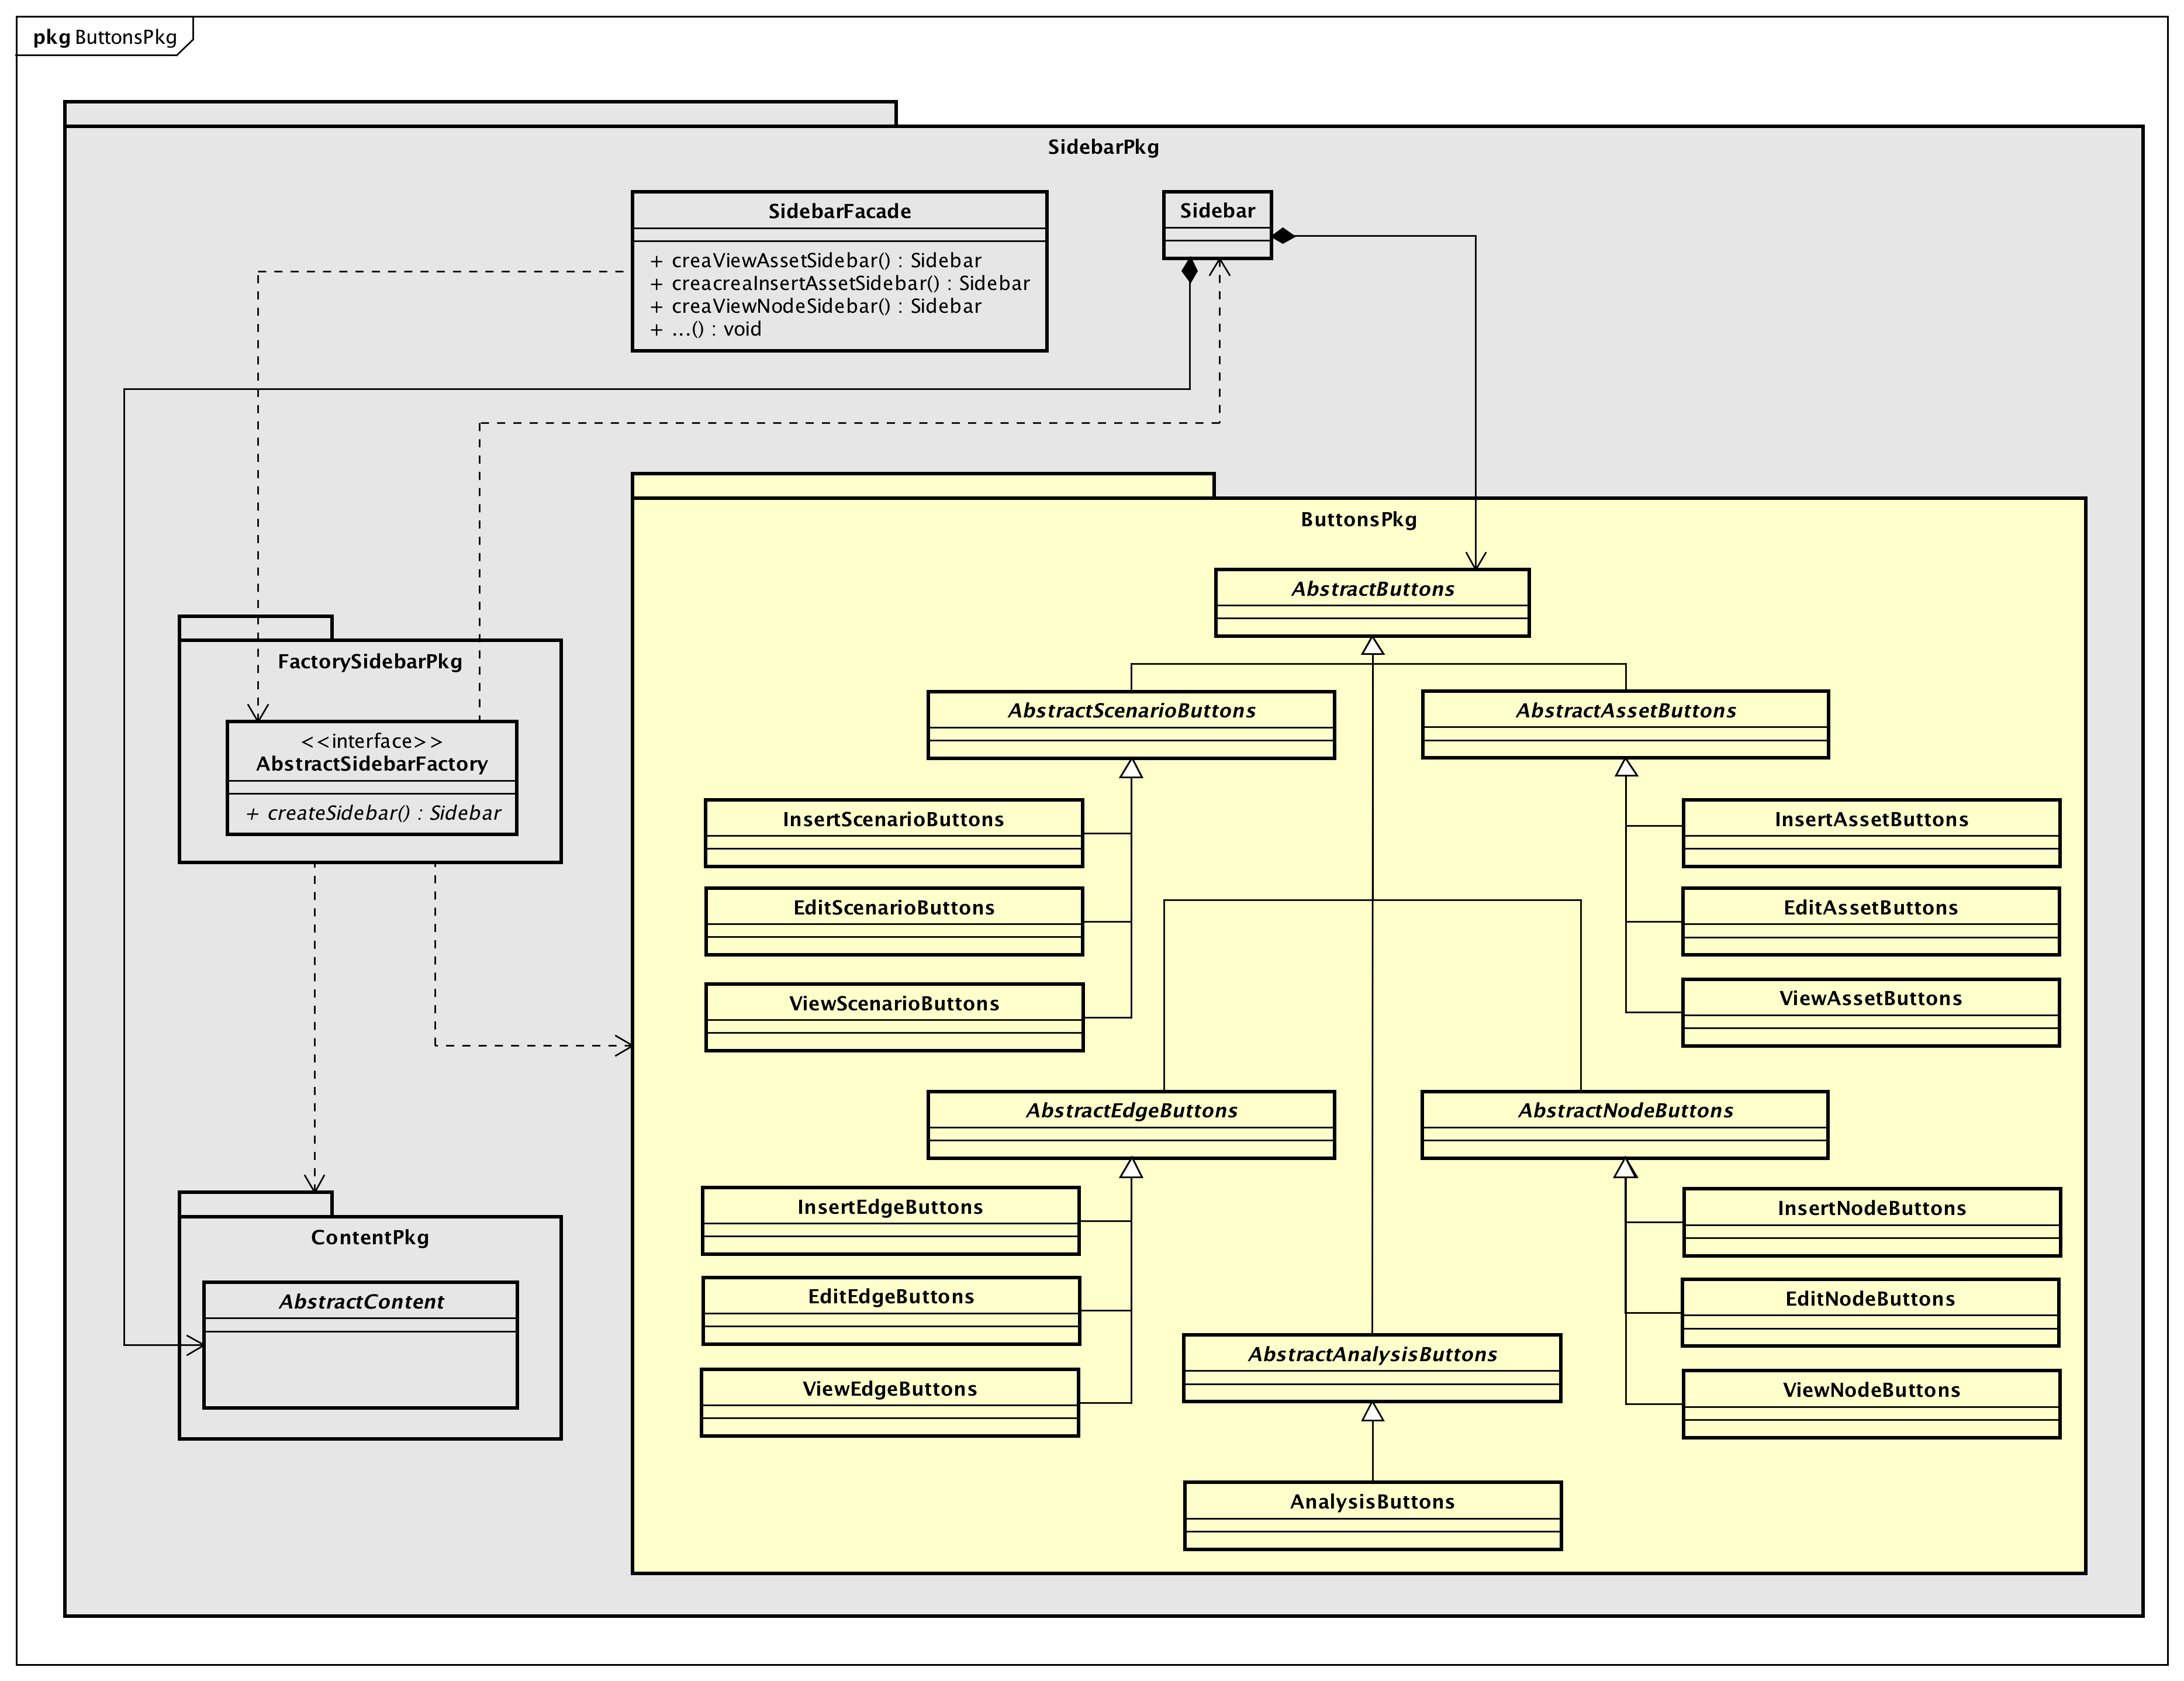
\includegraphics[width=\textwidth]{img/PkgDiagram/ButtonsPkg.png}
	\caption{Schema componente DeGeOP::ViewPkg::SidebarPkg::ButtonsPkg}
\end{figure}
\subsubsection{Informazioni sul package}
\begin{itemize}
	\item \textbf{descrizione:} racchiude le componenti che sono relative all'area con i bottoni della Sidebar;
	\item \textbf{padre:} \hyperref[pkg::SidebarPkg]{SidebarPkg};
	\item \textbf{classi contenute:}
	\begin{itemize}
		\item AbstractAnalysisButtons;
		\item AbstractAssetButtons;
		\item AbstractButtons;
		\item AbstractEdgeButtons;
		\item AbstractNodeButtons;
		\item AbstractScenarioButtons;
		\item AnalysisButtons;
		\item EditAssetButtons;
		\item EditEdgeButtons;
		\item EditNodeButtons;
		\item EditScenarioButtons;
		\item InsertAssetButtons;
		\item InsertEdgeButtons;
		\item InsertNodeButtons;
		\item InsertScenarioButtons;
		\item ViewAssetButtons;
		\item ViewEdgeButtons;
		\item ViewNodeButtons;
		\item ViewScenarioButtons.
	\end{itemize}
\end{itemize}
\subsubsection{Classi}
\paragraph{AbstractAnalysisButtons}
\begin{itemize}
	\item \textbf{descrizione:} una classe astratta rappresentante i bottoni della sidebar durante le operazioni sulle analisi;
	\item \textbf{utilizzo:} viene usata come interfaccia di specializzazione fra abstractButtons e le istanze di bottoni specifiche.
\end{itemize}
\paragraph{AbstractAssetButtons}
\begin{itemize}
	\item \textbf{descrizione:} una classe astratta rappresentante i bottoni della sidebar durante le operazioni sugli asset;
	\item \textbf{utilizzo:} viene usata come interfaccia di specializzazione fra abstractButtons e le istanze di bottoni specifiche.
\end{itemize}
\paragraph{AbstractButtons}
\begin{itemize}
	\item \textbf{descrizione:} una classe d'interfaccia rappresentante i bottoni inseriti nella sidebar;
	\item \textbf{utilizzo:} viene riferita da sidebar in quanto è una delle sue componenti;
	\item \textbf{relazioni con altre classi:} 
	\begin{itemize}
		\item IN Sidebar.
	\end{itemize}
\end{itemize}
\paragraph{AbstractEdgeButtons}
\begin{itemize}
	\item \textbf{descrizione:} una classe astratta rappresentante i bottoni della sidebar durante le operazioni sugli archi
	;
	\item \textbf{utilizzo:} viene usata come interfaccia di specializzazione fra abstractButtons e le istanze di bottoni specifiche.
\end{itemize}
\paragraph{AbstractNodeButtons}
\begin{itemize}
	\item \textbf{descrizione:} una classe astratta rappresentante i bottoni della sidebar durante le operazioni sui nodi
	;
	\item \textbf{utilizzo:} viene usata come interfaccia di specializzazione fra abstractButtons e le istanze di bottoni specifiche.
\end{itemize}
\paragraph{AbstractScenarioButtons}
\begin{itemize}
	\item \textbf{descrizione:} una classe astratta rappresentante i bottoni della sidebar durante le operazioni sugli scenari;
	\item \textbf{utilizzo:} viene usata come interfaccia di specializzazione fra abstractButtons e le istanze di bottoni specifiche.
\end{itemize}
\paragraph{AnalysisButtons}
\begin{itemize}
	\item \textbf{descrizione:} rappresenta i bottoni della sidebar relativi all'analisi di danno;
	\item \textbf{utilizzo:} viene creata da AnalysisFactory;
	\item \textbf{relazioni con altre classi:} 
	\begin{itemize}
		\item IN AnalysisSidebarFactory;
		\item OUT AnalysisActionCreator.
	\end{itemize}
\end{itemize}
\paragraph{EditAssetButtons}
\begin{itemize}
	\item \textbf{descrizione:} rappresenta i bottoni della sidebar relativi alla modifica di un asset;
	\item \textbf{utilizzo:} viene creata da EditAssetFactory;
	\item \textbf{relazioni con altre classi:} 
	\begin{itemize}
		\item IN EditAssetSidebarFactory;
		\item OUT AssetActionCreator.
	\end{itemize}
\end{itemize}
\paragraph{EditEdgeButtons}
\begin{itemize}
	\item \textbf{descrizione:} rappresenta i bottoni della sidebar relativi alla modifica di un arco;
	\item \textbf{utilizzo:} viene creata da EditEdgeFactory;
	\item \textbf{relazioni con altre classi:} 
	\begin{itemize}
		\item IN EditEdgeSidebarFactory;
		\item OUT EdgeActionCreator.
	\end{itemize}
\end{itemize}
\paragraph{EditNodeButtons}
\begin{itemize}
	\item \textbf{descrizione:} rappresenta i bottoni della sidebar relativi alla modifica di un nodo;
	\item \textbf{utilizzo:} viene creata da EditNodeFactory;
	\item \textbf{relazioni con altre classi:} 
	\begin{itemize}
		\item IN EditNodeSidebarFactory;
		\item OUT NodeActionCreator.
	\end{itemize}
\end{itemize}
\paragraph{EditScenarioButtons}
\begin{itemize}
	\item \textbf{descrizione:} rappresenta i bottoni della sidebar relativi alla modifica di uno scenario di danno;
	\item \textbf{utilizzo:} viene creata da EditScenarioFactory;
	\item \textbf{relazioni con altre classi:} 
	\begin{itemize}
		\item IN EditScenarioSidebarFactory;
		\item OUT ScenarioActionCreator.
	\end{itemize}
\end{itemize}
\paragraph{InsertAssetButtons}
\begin{itemize}
	\item \textbf{descrizione:} rappresenta i bottoni della sidebar relativi all'inserimento di un asset;
	\item \textbf{utilizzo:} viene creata da InsertAssetFactory;
	\item \textbf{relazioni con altre classi:} 
	\begin{itemize}
		\item IN InsertAssetSidebarFactory;
		\item OUT AssetActionCreator.
	\end{itemize}
\end{itemize}
\paragraph{InsertEdgeButtons}
\begin{itemize}
	\item \textbf{descrizione:} rappresenta i bottoni della sidebar relativi all'inserimento di un arco;
	\item \textbf{utilizzo:} viene creata da InsertEdgeFactory;
	\item \textbf{relazioni con altre classi:} 
	\begin{itemize}
		\item IN InsertEdgeSidebarFactory;
		\item OUT EdgeActionCreator.
	\end{itemize}
\end{itemize}
\paragraph{InsertNodeButtons}
\begin{itemize}
	\item \textbf{descrizione:} rappresenta i bottoni della sidebar relativi all'inserimento di un nodo;
	\item \textbf{utilizzo:} viene creata da InsertNodeFactory;
	\item \textbf{relazioni con altre classi:} 
	\begin{itemize}
		\item IN InsertNodeSidebarFactory;
		\item OUT NodeActionCreator.
	\end{itemize}
\end{itemize}
\paragraph{InsertScenarioButtons}
\begin{itemize}
	\item \textbf{descrizione:} rappresenta i bottoni della sidebar relativa all'inserimento di uno scenario di danno;
	\item \textbf{utilizzo:} viene creata da InsertScenarioFactory;
	\item \textbf{relazioni con altre classi:} 
	\begin{itemize}
		\item IN InsertScenarioSidebarFactory;
		\item OUT ScenarioActionCreator.
	\end{itemize}
\end{itemize}
\paragraph{ViewAssetButtons}
\begin{itemize}
	\item \textbf{descrizione:} rappresenta i bottoni della sidebar relativi alla visualizzazione di un asset;
	\item \textbf{utilizzo:} viene creata da ViewAssetFactory;
	\item \textbf{relazioni con altre classi:} 
	\begin{itemize}
		\item IN ViewAssetSidebarFactory;
		\item OUT AssetActionCreator.
	\end{itemize}
\end{itemize}
\paragraph{ViewEdgeButtons}
\begin{itemize}
	\item \textbf{descrizione:} rappresenta i bottoni della sidebar relativi alla visualizzazione di un arco;
	\item \textbf{utilizzo:} viene creata da ViewEdgeFactory;
	\item \textbf{relazioni con altre classi:} 
	\begin{itemize}
		\item IN ViewEdgeSidebarFactory;
		\item OUT EdgeActionCreator.
	\end{itemize}
\end{itemize}
\paragraph{ViewNodeButtons}
\begin{itemize}
	\item \textbf{descrizione:} rappresenta i bottoni della sidebar relativi alla visualizzazione di un nodo;
	\item \textbf{utilizzo:} viene creata da ViewNodeFactory;
	\item \textbf{relazioni con altre classi:} 
	\begin{itemize}
		\item IN ViewNodeSidebarFactory;
		\item OUT NodeActionCreator.
	\end{itemize}
\end{itemize}
\paragraph{ViewScenarioButtons}
\begin{itemize}
	\item \textbf{descrizione:} rappresenta i bottoni della sidebar relativi alla visualizzazione di uno scenario di danno;
	\item \textbf{utilizzo:} viene creata da ViewScenarioFactory;
	\item \textbf{relazioni con altre classi:} 
	\begin{itemize}
		\item IN ViewScenarioSidebarFactory;
		\item OUT ScenarioActionCreator.
	\end{itemize}
\end{itemize}
\newpage



	\newpage

\section{Stime di fattibilità e bisogno di risorse}
\label{sec:sdf}

L'architettura definita precedentemente ha raggiunto un livello di dettaglio sufficiente a fornire una stima sulla fattibilità e di bisogno di risorse.
Durante la progettazione iniziale del prodotto e la scelta delle tecnologie da utilizzare, si sono riscontrati diversi potenziali limiti legati agli stessi.
Il \glo{Gruppo}{gruppo} si è impegnato a coprire le parti carenti come descritto nei paragrafi sottostanti, al fine di rendere le tecnologie completamente adeguate per la realizzazione del prodotto.

\subsection{JavaScript}

L'utilizzo ottimale di \glo{Libreria}{librerie} come \glo{React}{React} e Redux prevedono l'uso di costrutti e sintassi presenti solo dalla versione ES6 di \glo{JavaScript}{JavaScript} in poi. Tale versione non è ancora totalmente definita e quindi molti browser odierni non supportano nativamente alcune feature. Specificatamente ES6 ha inserito la sintassi relativa al costrutto delle classi (class, construct, ecc.) e alcuni operatori utili all'implementazione dei \glo{Reducer}{reducer} in Redux (per esempio lo spread operator). Questa situazione ha portato ad una serie di conseguenze, fra le quali:
\begin{itemize}
	\item utilizzo di Babel, una \glo{Componente}{componente} \js{} che agisce come compilatore (o meglio, come un refactor di codice) trasformando codice, che utilizza le feature definite in ES6 o superiore, in codice completamente compatibile alla versione ES5, che quindi è supportato nativamente dai browser moderni;
	\item bassa presenza di codice e librerie scritte in ES6. Per esempio la libreria OpenLayer e la sua documentazione sono scritte in codice ES5. Ciò si ripercuote sul prodotto da definire in due modi:
	\begin{itemize}
		\item necessità di convertire il codice ES5 in codice ES6 per mantenere uniforme il codice prodotto;
		\item necessità di importare librerie secondarie che operano tale conversione liberando il team dalla scrittura di ulteriore codice.
	\end{itemize}
\end{itemize}
Il \glo{Package}{package} Babel è una componente popolare e molto usata quindi il rischio che  non funzioni correttamente è molto basso, ma comunque da non trascurare.

\subsection{React}

La libreria React è relativamente giovane, ma risulta molto usata. Risulta essere soprattutto una libreria stabile, anche a causa del numero basso di \glo{Issue}{issue} correttamente aperti sulla relativa pagina \glo{Github}{GitHub}.
\\Il requisito di funzionamento del prodotto su dispositivi mobile, nello specifico su tablet, implica che il prodotto stesso dovrebbe risultare di piccole dimensioni e computazionalmente leggero, per favorire un uso veloce e fluido anche su questa famiglia di dispositivi. React risulta una libreria adatta allo scopo in quanto leggera e pienamente supportata su dispositivi mobili. 
	\newpage
\section{Attività}
\subsection{Introduzione}
Questa sezione descriverà le operazioni che l'utente può svolgere all'interno di \progetto.
\\Per ogni operazione viene fornita:
\begin{itemize}
	\item una descrizione;
	\item un diagramma di attività;
	\item uno o più eventuali mockup.
\end{itemize}
I mockup hanno lo scopo di chiarificare la struttura della single-page \progetto. Il gruppo si riserva di poter modificare alcuni elementi grafici quando il prodotto sarà progettato nel dettaglio.
\\Le operazioni più complesse nei diagrammi di attività presentano uno sfondo di colore azzurro e sono ulteriormente descritte da sotto-diagrammi. \\ \\
%
Di seguito vengono mostrati due mockup che evidenziano come verrà organizzata l'interfaccia grafica nel progetto \progetto.
\begin{figure}[H]
	\centering
	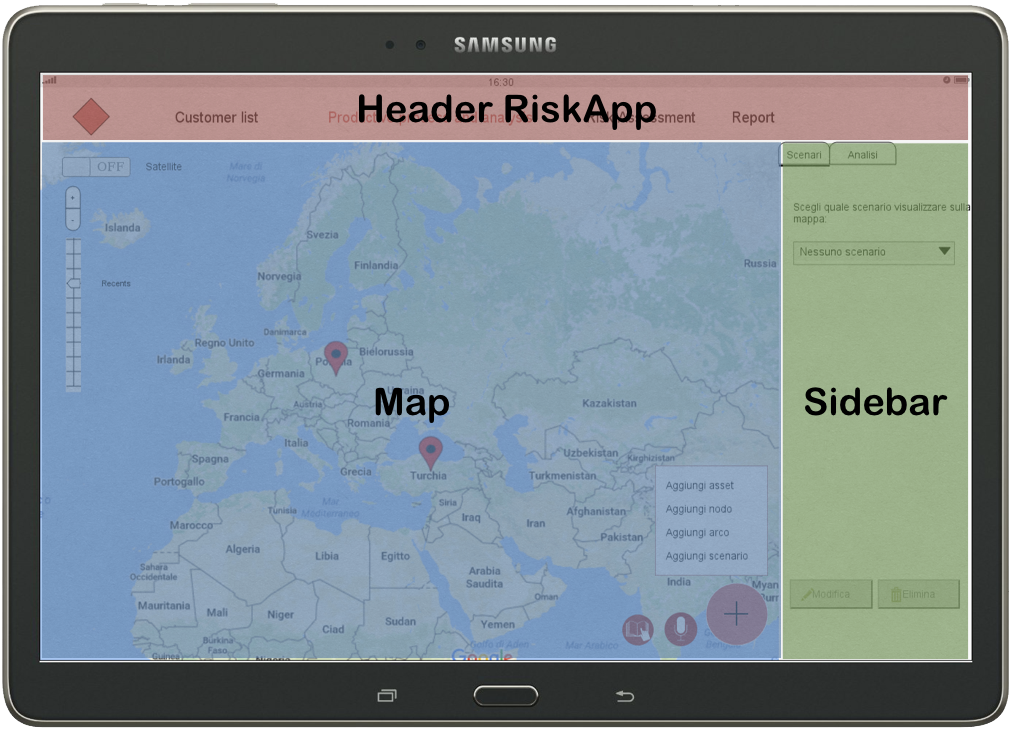
\includegraphics[scale=0.4]{img/MockUp/MockupConLayerHi}
	\caption{Mockup interfaccia grafica ad alto livello}
\end{figure}

\begin{figure}[H]
	\centering
	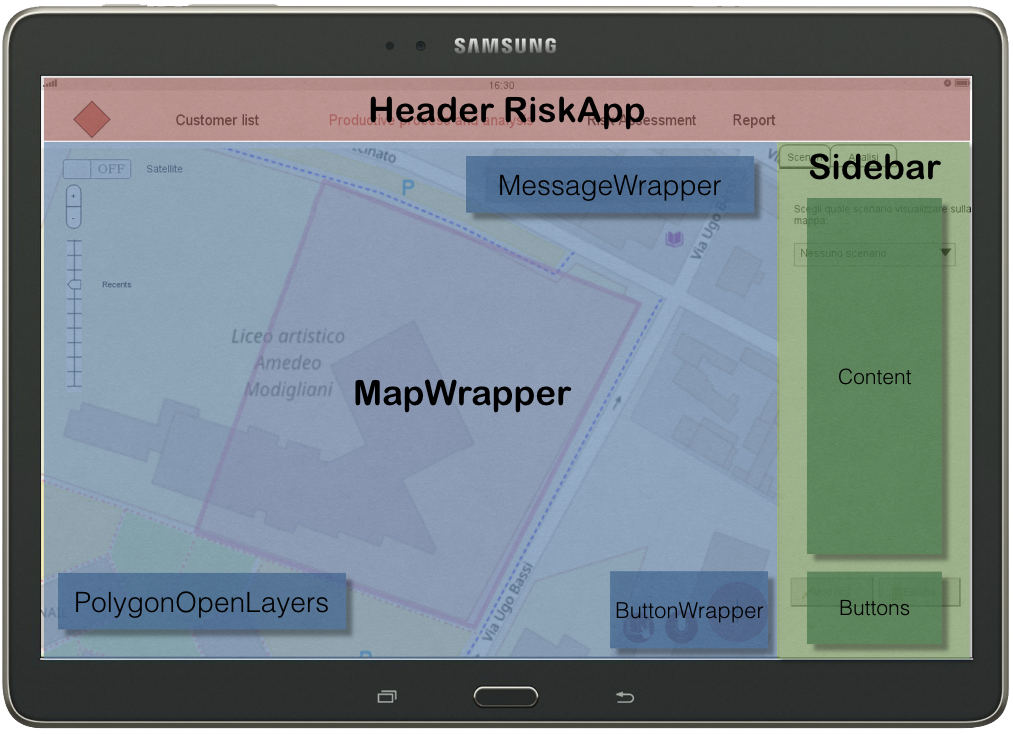
\includegraphics[scale=0.4]{img/MockUp/MockupConLayerLow}
	\caption{Mockup interfaccia grafica basso livello}
\end{figure}

\subsection{Visualizzazione di default}
\progetto{} sarà sviluppato come una single-page e tutte le operazioni che l'utente può svolgere sono attuabili a partire dalla visualizzazione di default (si veda il relativo mockup).
L'utente, dopo aver acceduto a \progetto, potrà:
\begin{itemize}
	\item interagire ripetutamente con la mappa:
		\begin{itemize}
			\item aumentando/diminuendo il livello di zoom;
			\item spostandosi sulla mappa;
			\item attivando/disattivando la vista satellitare.
		\end{itemize}
	\item svolgere ripetutamente una o più tra le seguenti operazioni:
	\begin{itemize}
		\item selezionare un asset, nodo, arco, scenario;
		\item aggiungere asset, nodi, archi, scenari;
		\item gestire le analisi;
		\item avviare il tutorial o l'assistente vocale.
	\end{itemize}
\end{itemize} 



\begin{figure}[H]
	\centering
	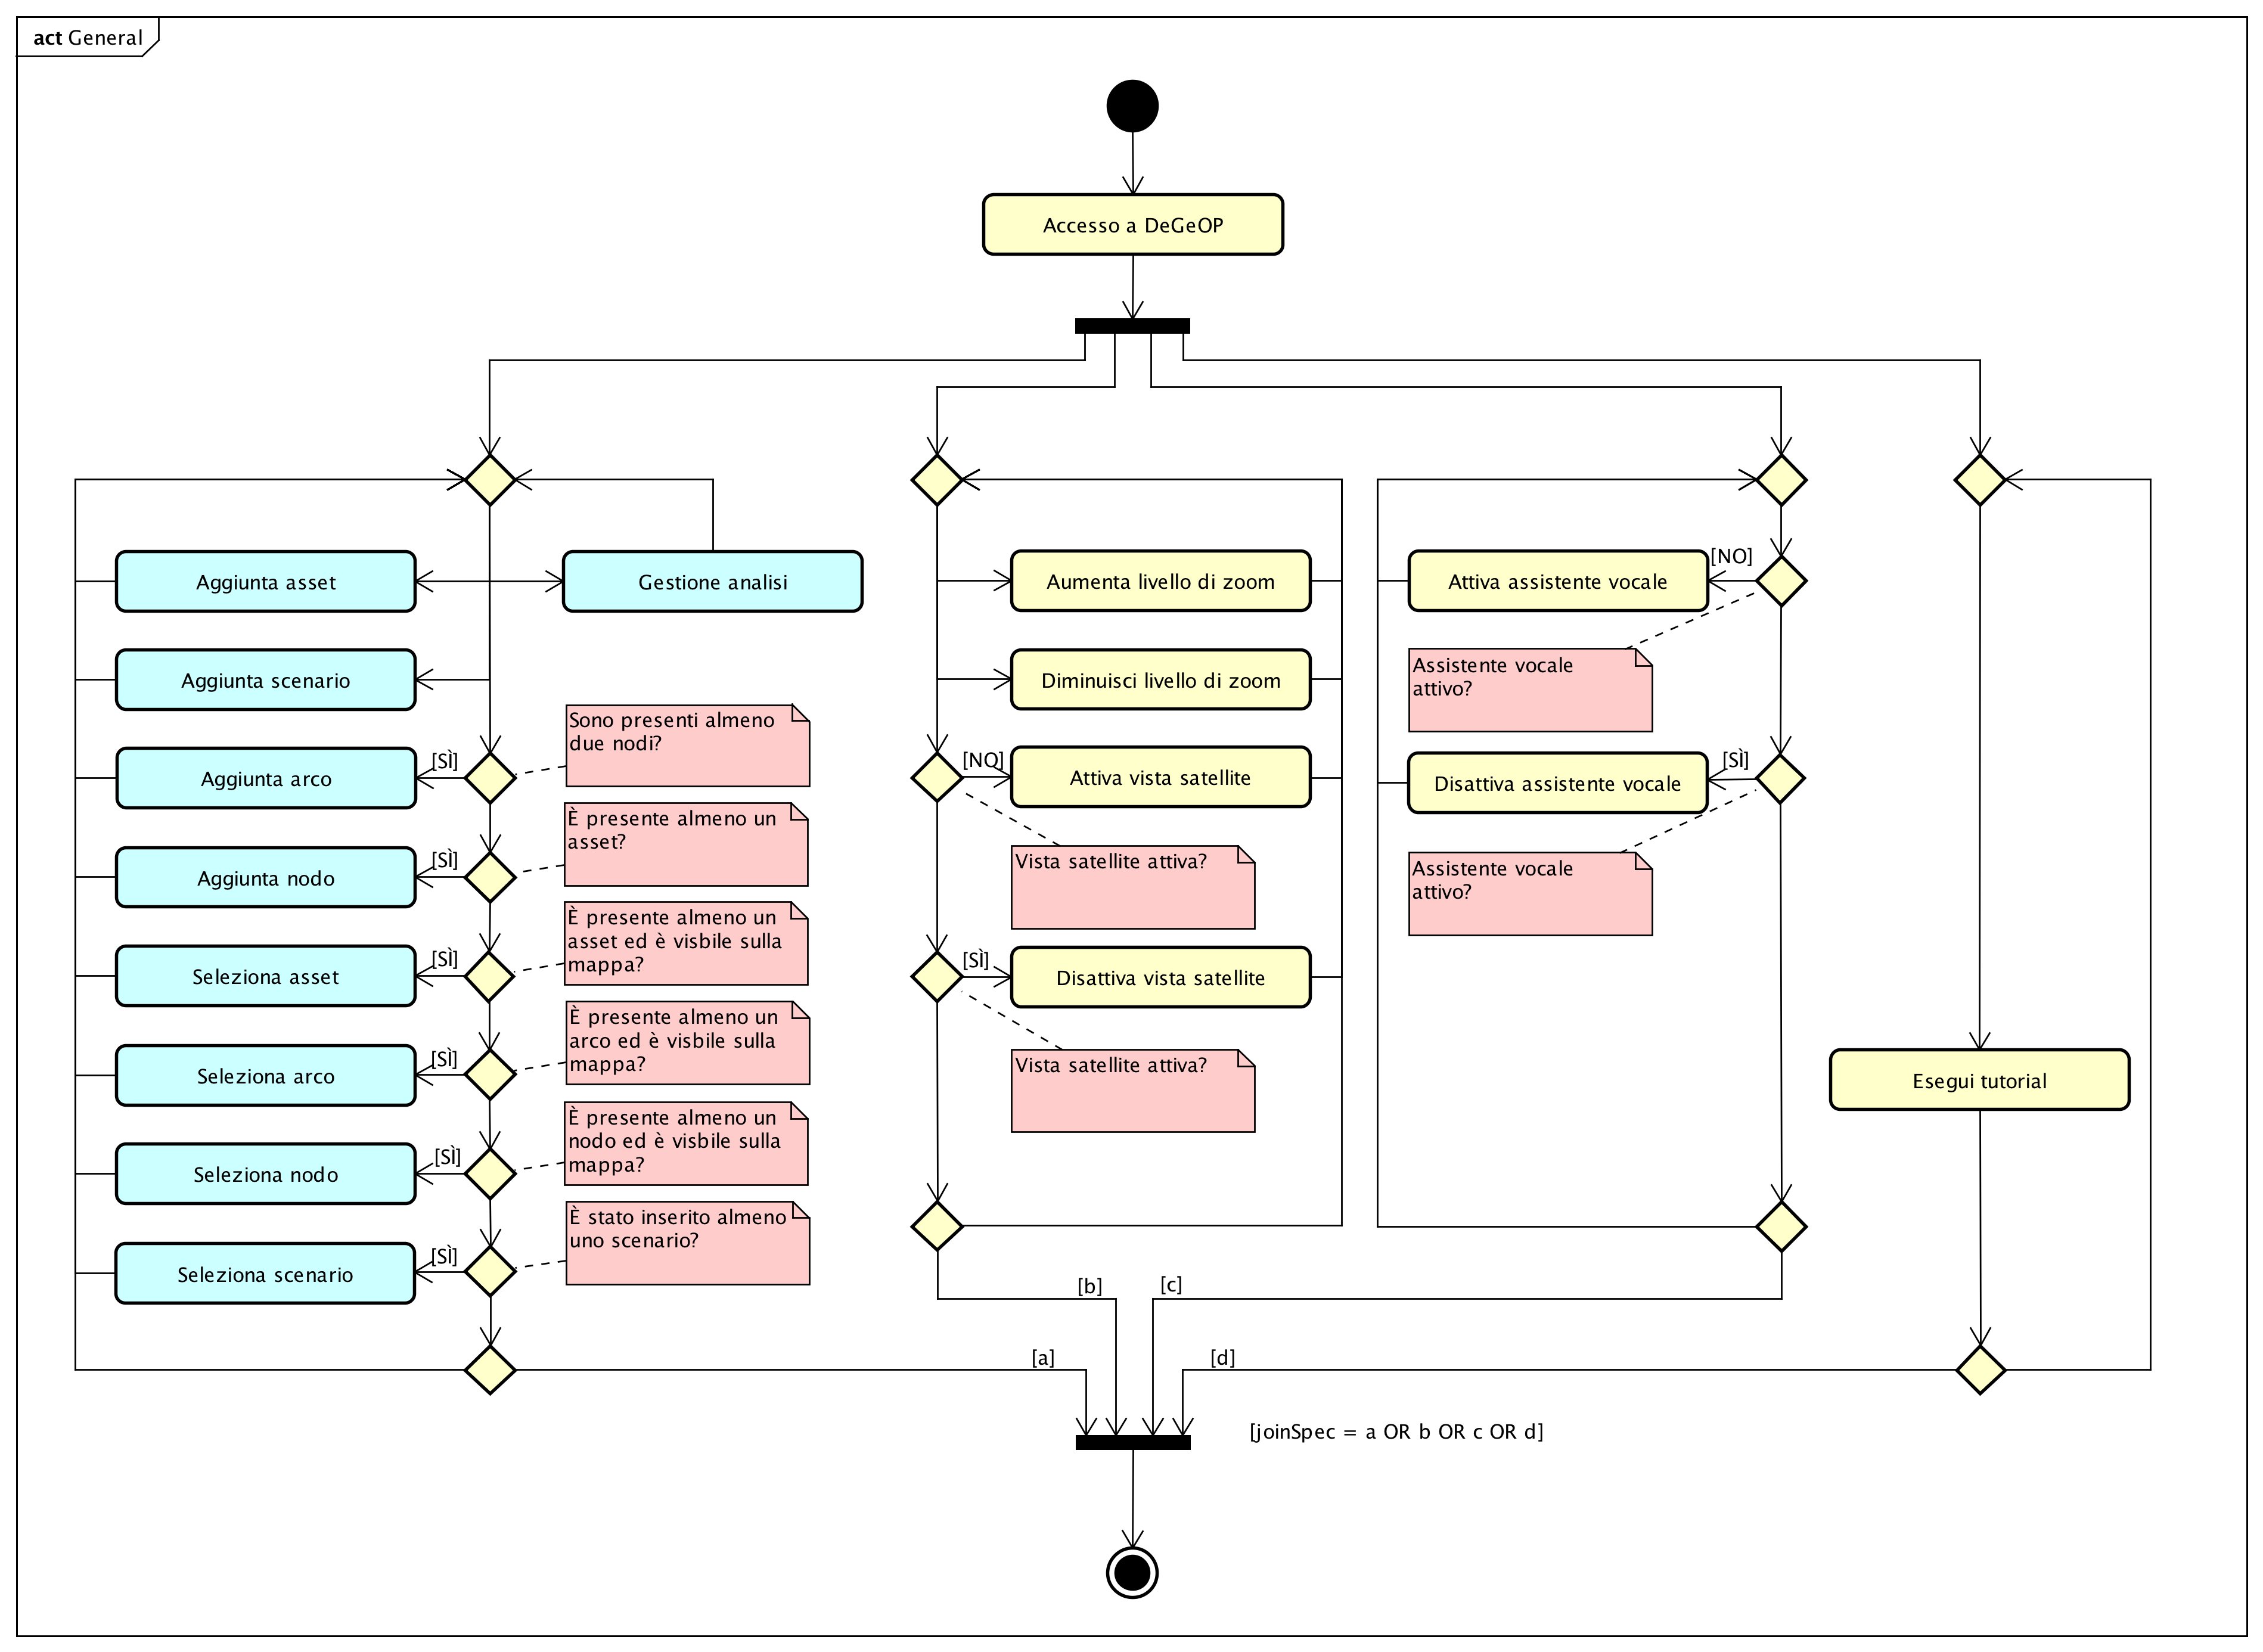
\includegraphics[width=\textwidth]{img/DiagrammiDiAttivita/GeneralActivities.png}
	\caption{Diagramma delle attività generale}
\end{figure}

\begin{figure}[H]
	\centering
	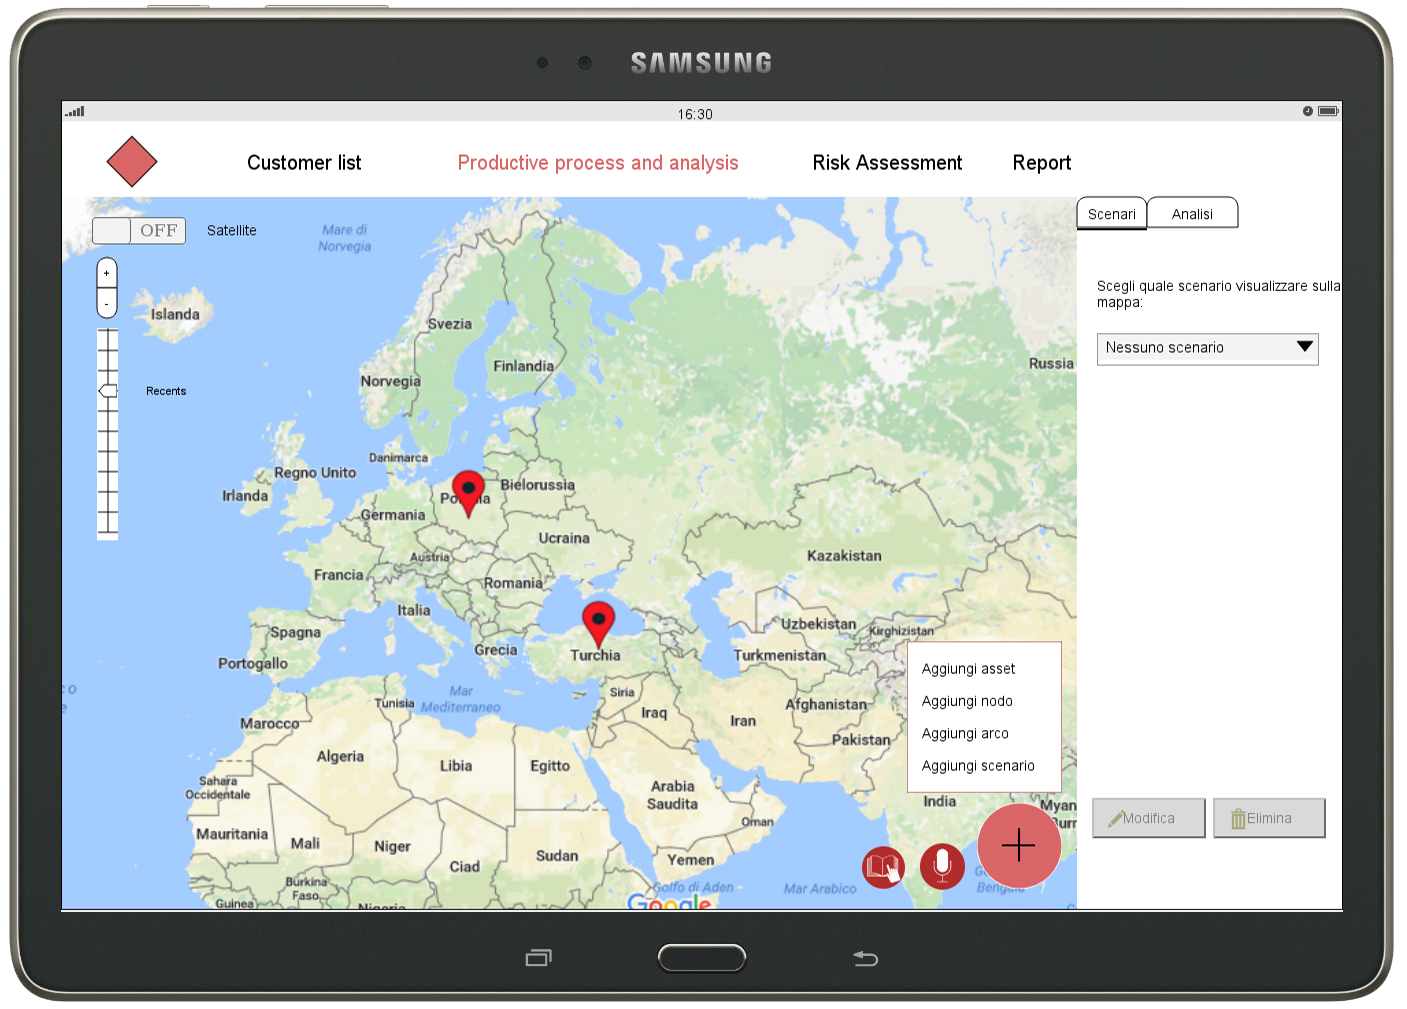
\includegraphics[width=\textwidth]{img/MockUp/m0.jpg}
	\caption{Mockup per la visualizzazione di default}
\end{figure}

\newpage
\subsection{Aggiunta asset}
Per aggiungere un asset l'utente dovrà disegnare il perimetro dell'asset sulla mappa, compilarne i dati e confermare l'inserimento. In caso di dati non corretti, l'inserimento potrebbe non andare a buon fine: verrà visualizzato un messaggio di errore e l'utente sarà tenuto a correggere eventuali errori o incompletezze.
In ogni momento l'utente può annullare l'inserimento. Il sistema richiede una conferma per portare a termine tale operazione. 
\begin{figure}[H]
	\centering
	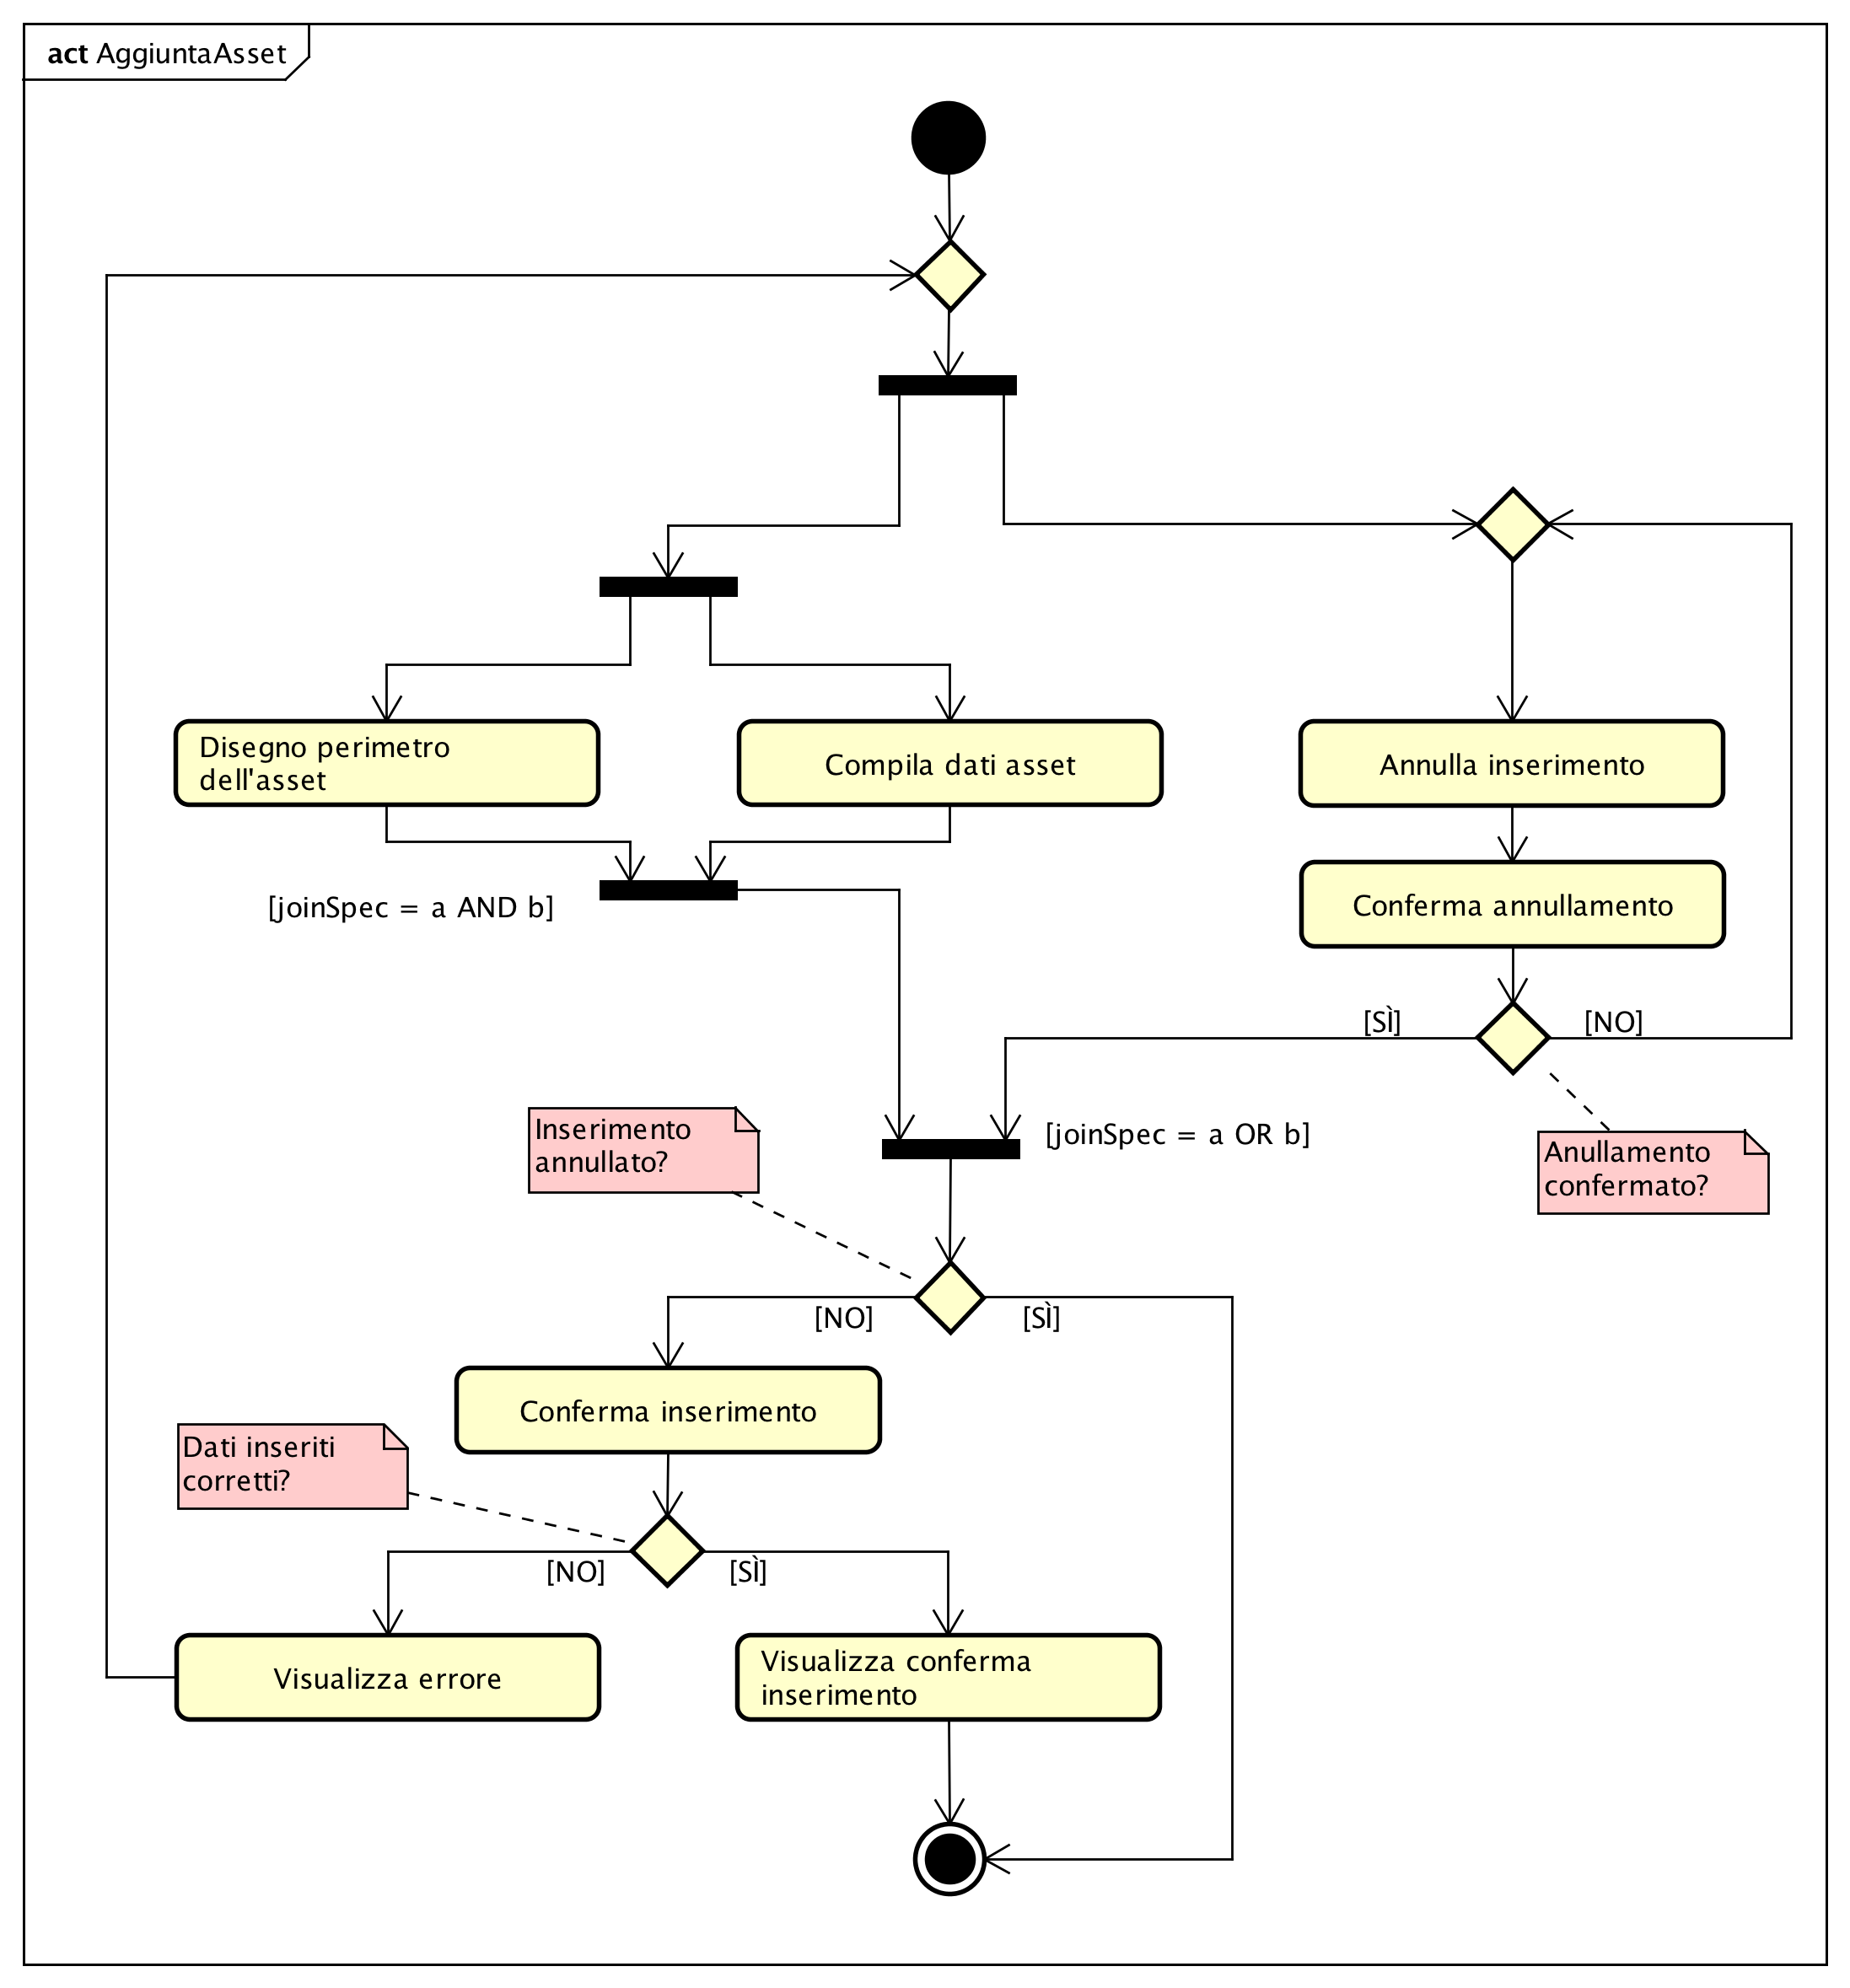
\includegraphics[width=\textwidth]{img/DiagrammiDiAttivita/AggiuntaAsset.png}
	\caption{Diagramma di attività per l'aggiunta di un asset}
\end{figure}
\begin{figure}[H]
	\centering
	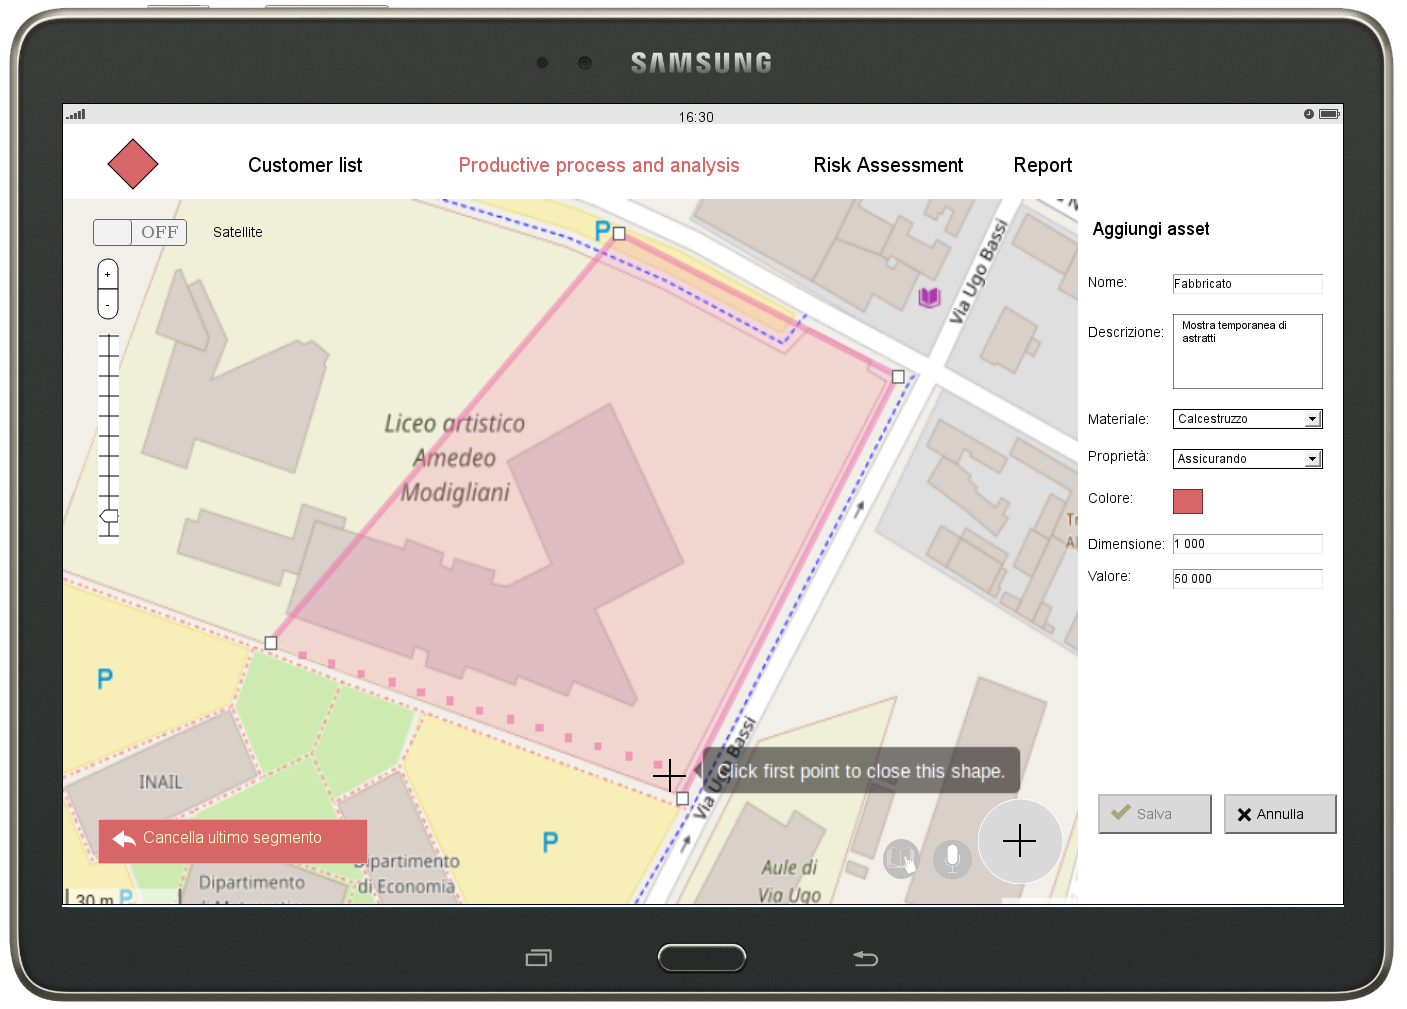
\includegraphics[scale=0.29]{img/MockUp/m4.png}
	\caption{Mockup per l'aggiunta dell'asset}
\end{figure}
\begin{figure}[H]
	\centering
	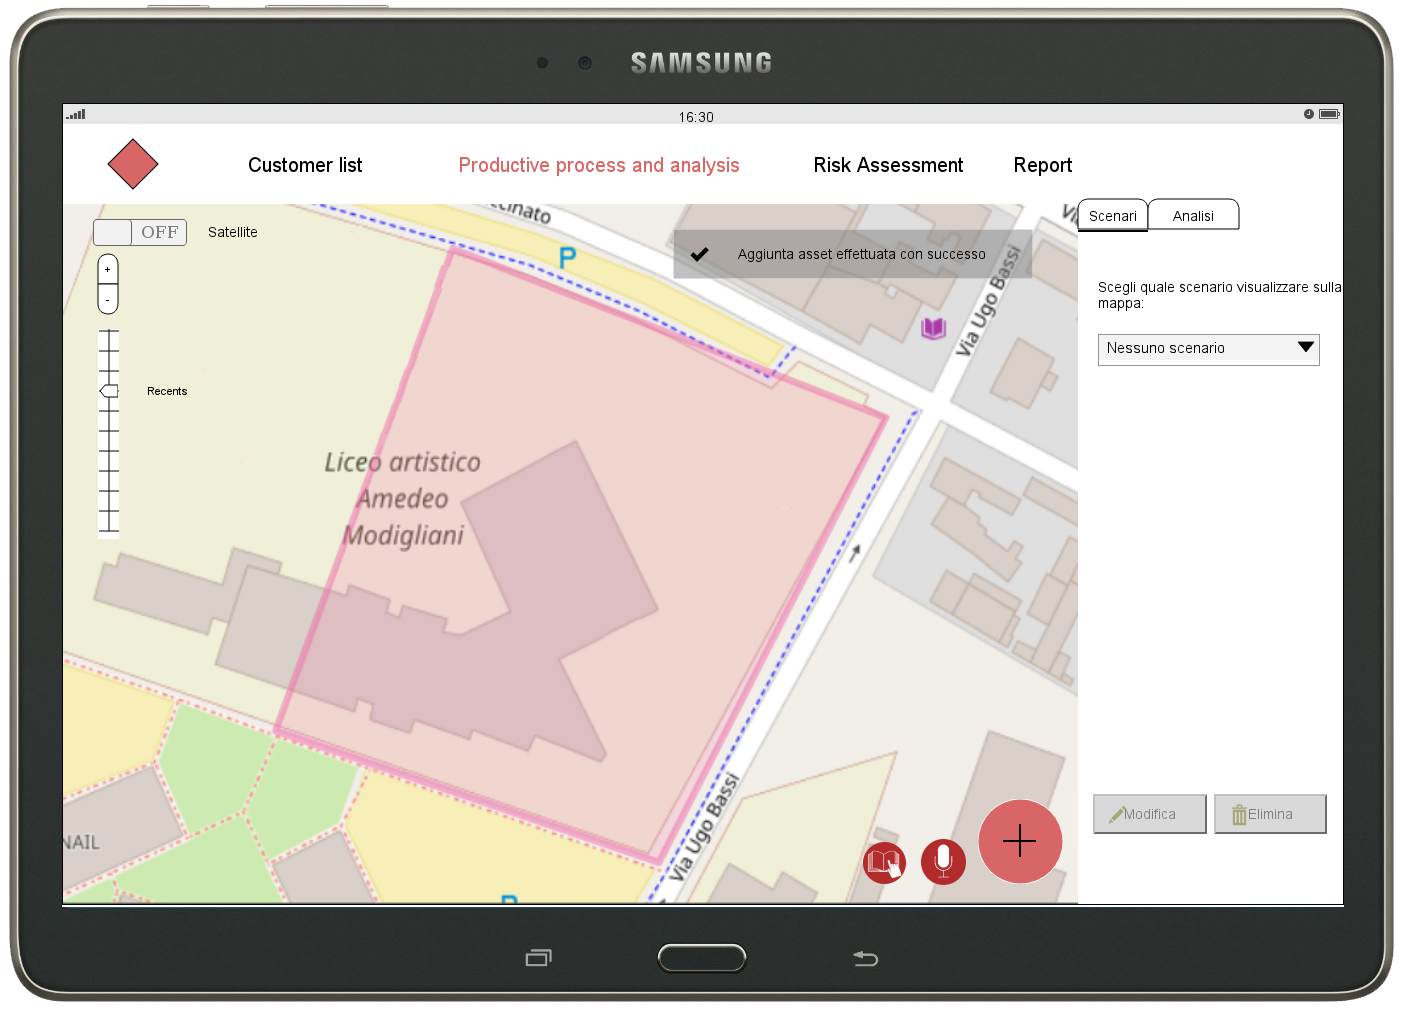
\includegraphics[scale=0.29]{img/MockUp/m5.png}
	\caption{Mockup per il successo dell'operazione di aggiunta asset}
\end{figure}
\begin{figure}[H]
	\centering
	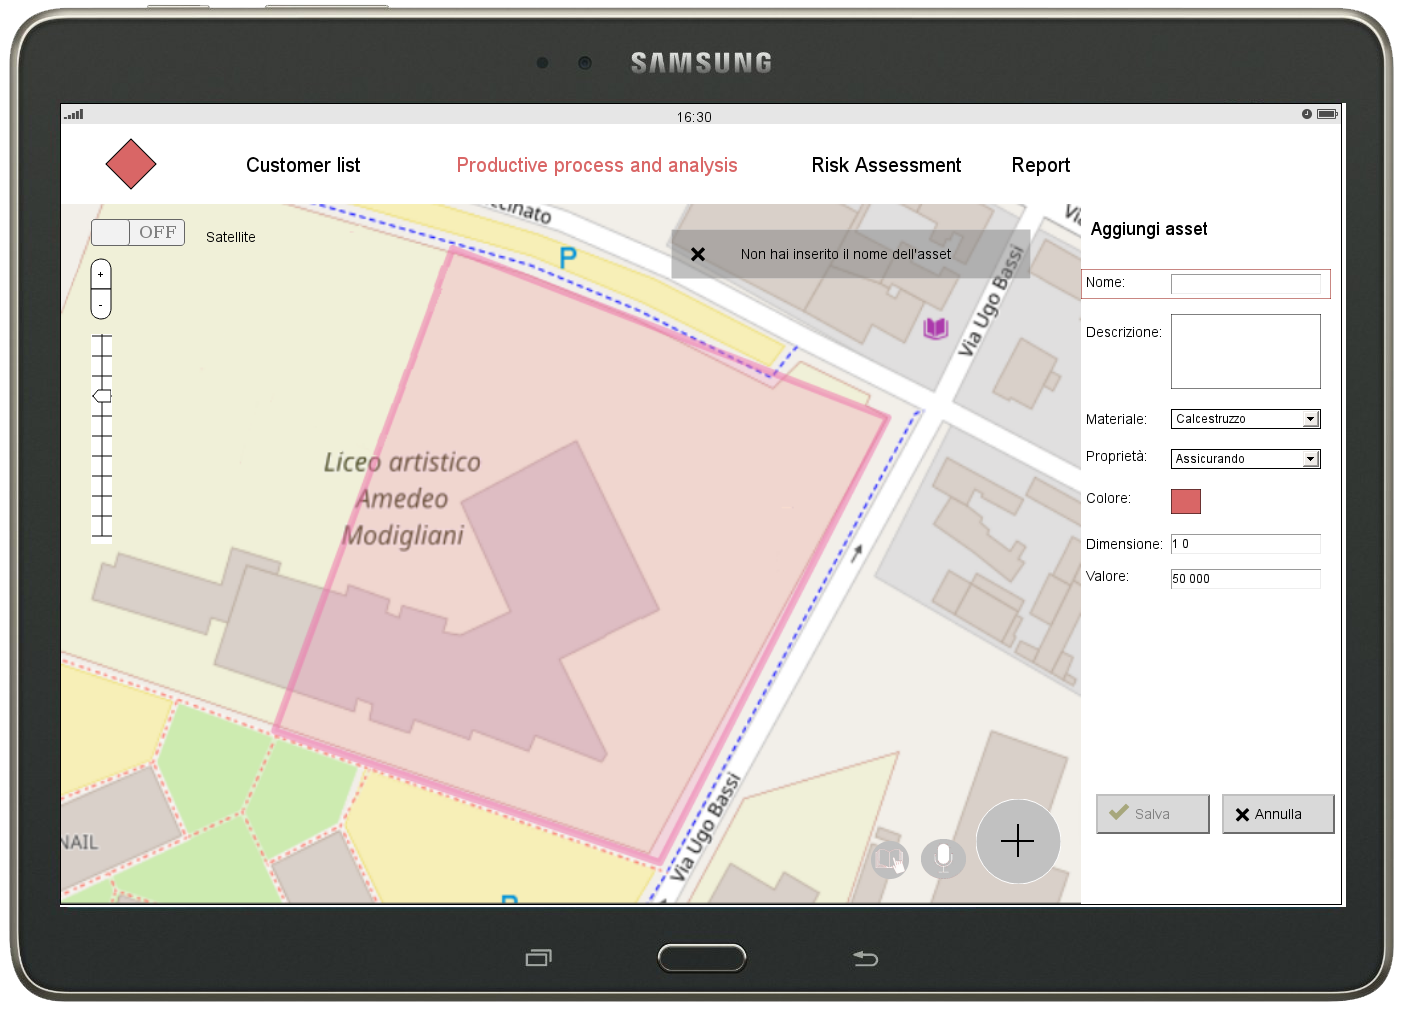
\includegraphics[scale=0.29]{img/MockUp/m6.png}
	\caption{Mockup per l'errore durante l'operazione di aggiunta asset}
\end{figure}

\newpage
\subsection{Aggiunta nodo}
Per aggiungere un nodo, l'utente dovrà posizionare il nodo all'interno dell'asset di appartenenza sulla mappa, compilarne i dati e confermare l'inserimento. In caso di dati non corretti, l'inserimento potrebbe non andare a buon fine: verrà visualizzato un messaggio di errore e l'utente sarà tenuto a correggere eventuali errori o incompletezze.
In ogni momento l'utente può annullare l'inserimento. Il sistema richiede una conferma per portare a termine tale operazione. 
\begin{figure}[H]
	\centering
	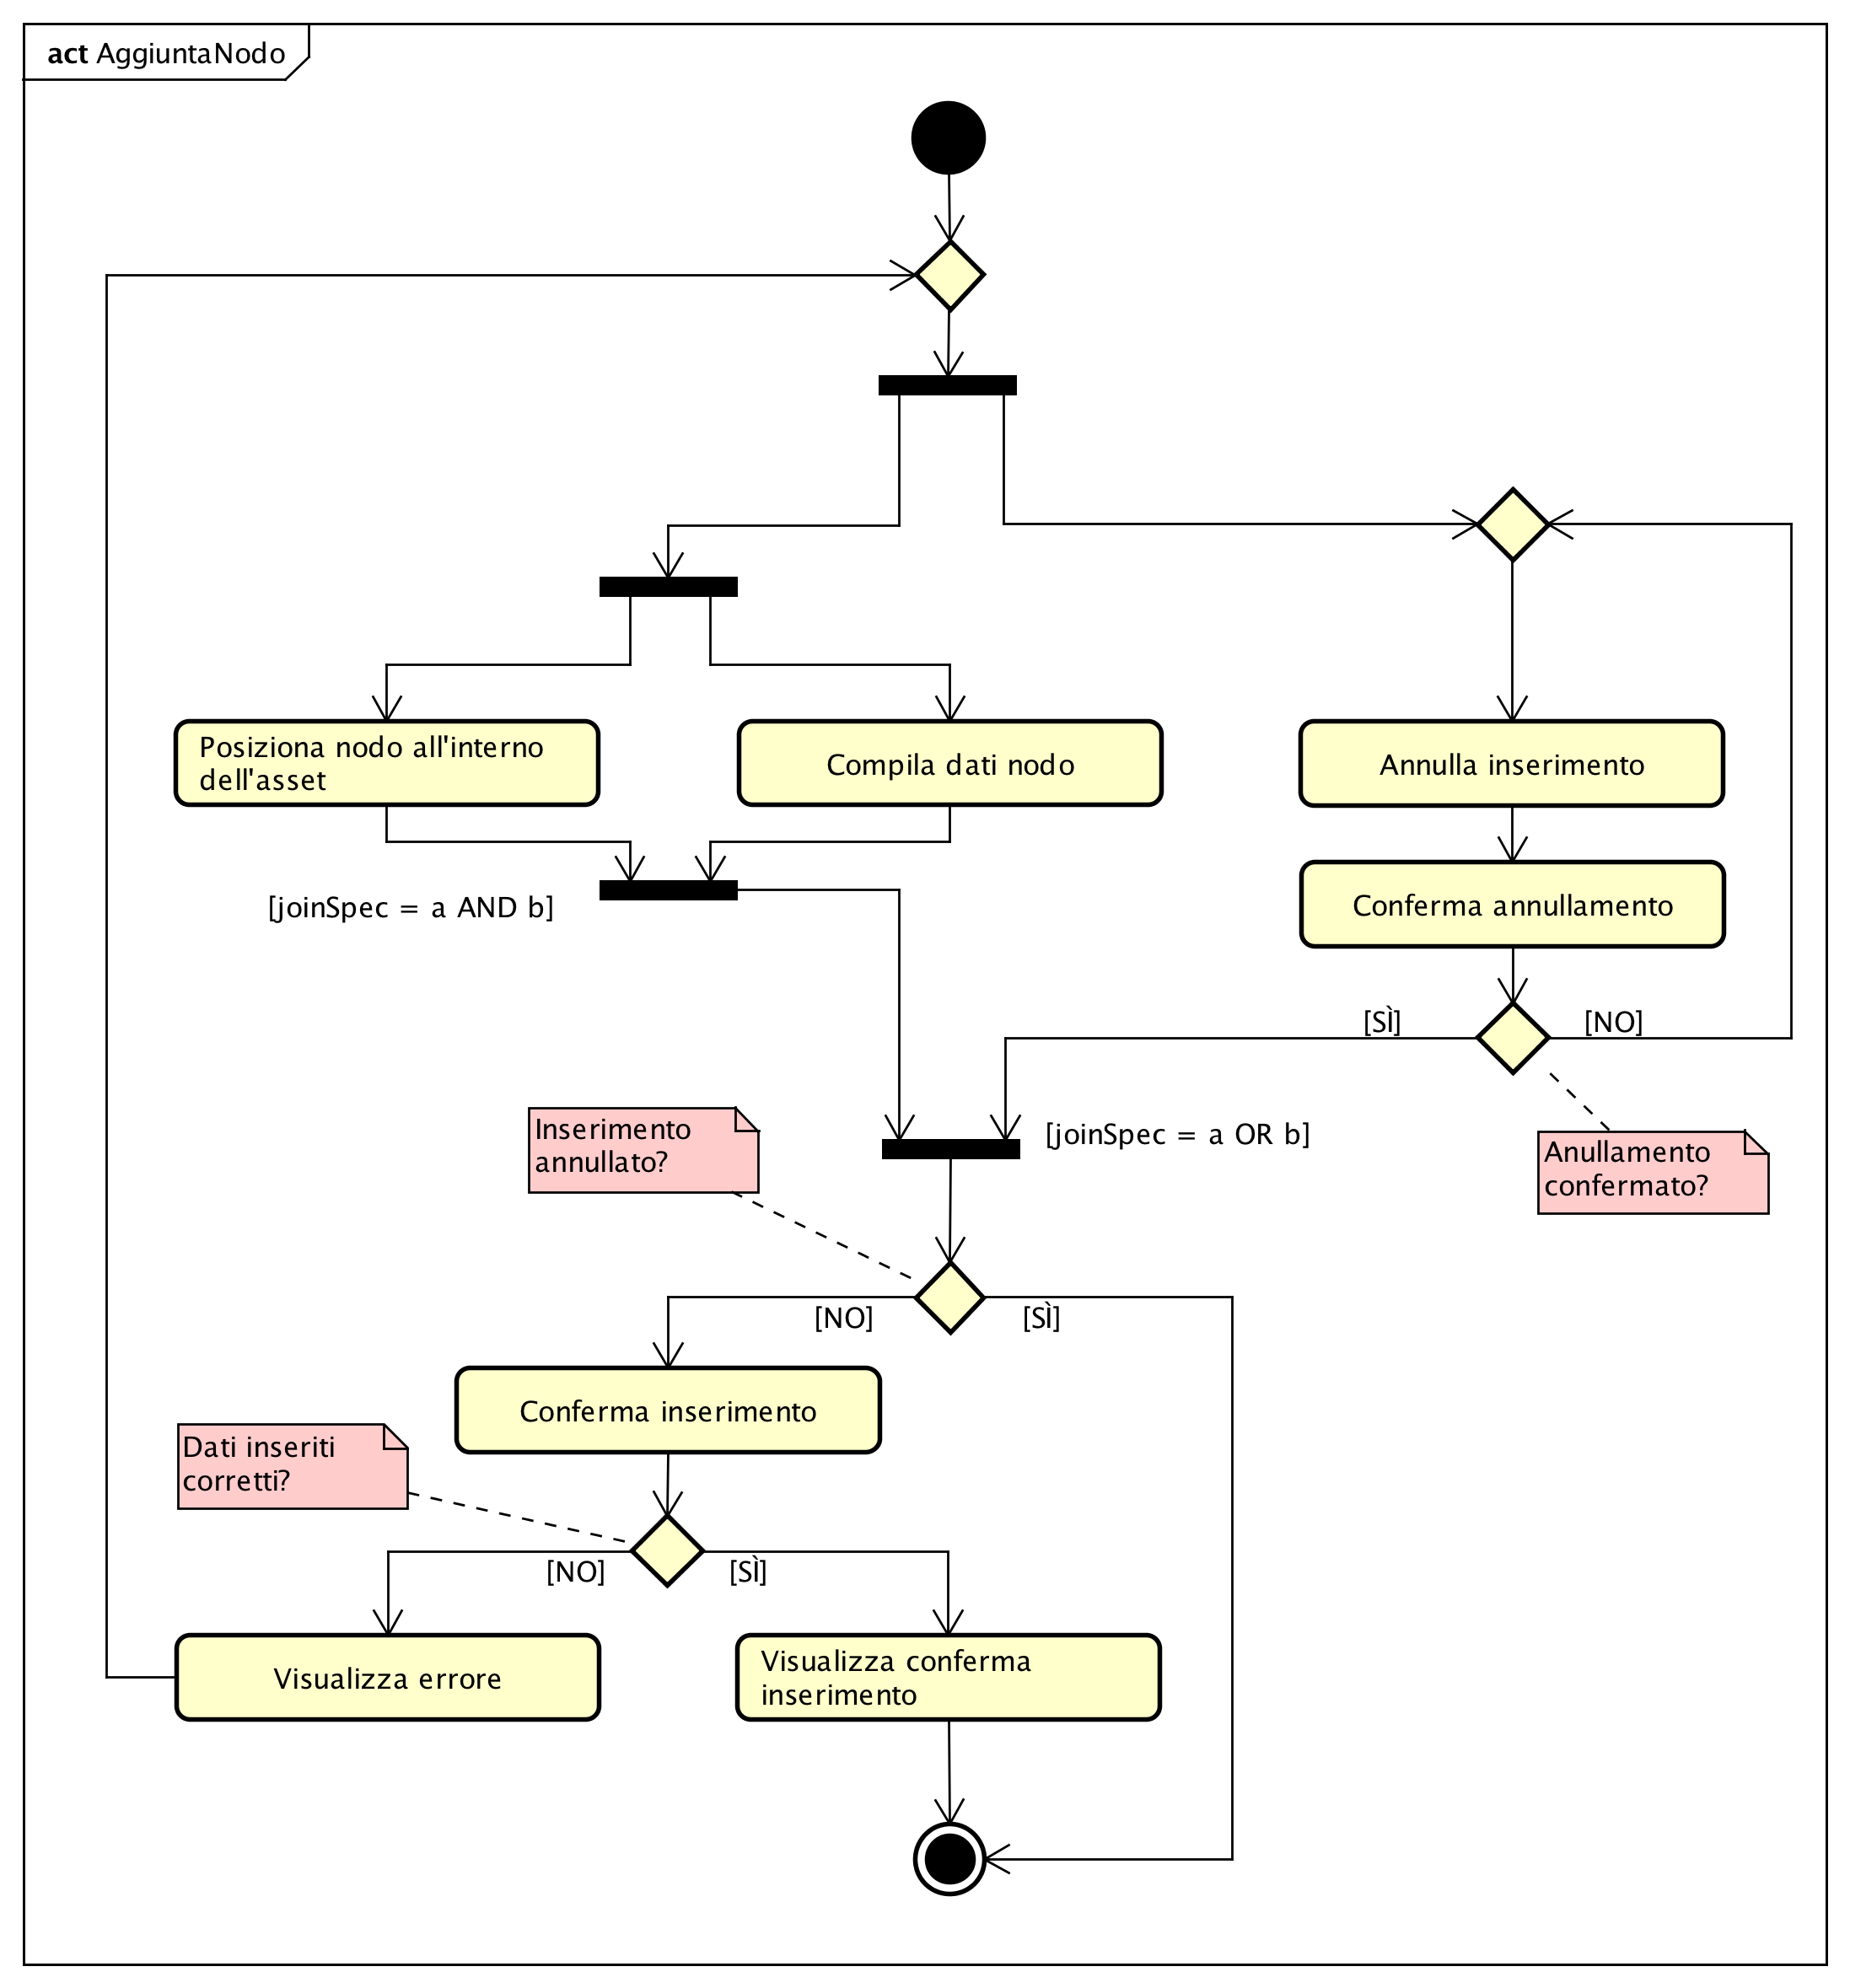
\includegraphics[width=\textwidth]{img/DiagrammiDiAttivita/AggiuntaNodo.png}
	\caption{Diagramma di attività per l'aggiunta di un nodo}
\end{figure}
\begin{figure}[H]
	\centering
	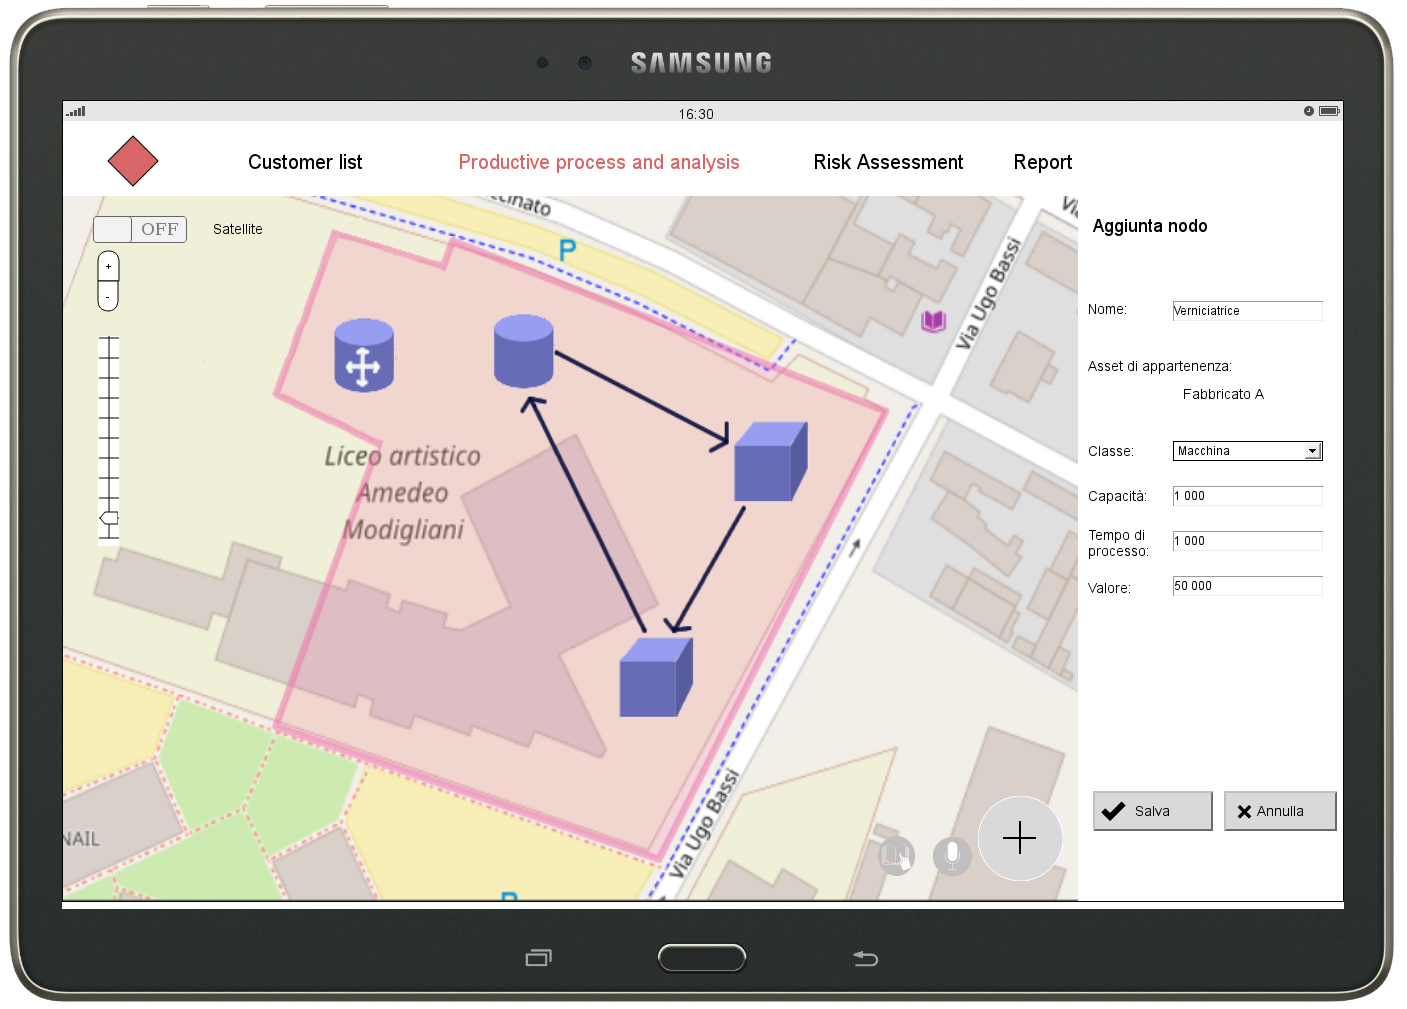
\includegraphics[width=\textwidth]{img/MockUp/m12.png}
	\caption{Mockup per l'aggiunta di un nodo}
\end{figure}

\newpage
\subsection{Aggiunta arco}
Per aggiungere un arco, l'utente dovrà disegnare l'arco sulla mappa, compilarne i dati e confermare l'inserimento. In caso di dati non corretti, l'inserimento potrebbe non andare a buon fine: verrà visualizzato un messaggio di errore e l'utente sarà tenuto a correggere eventuali errori o incompletezze.
In ogni momento l'utente può annullare l'inserimento. Il sistema richiede una conferma per portare a termine tale operazione.
\begin{figure}[H]
	\centering
	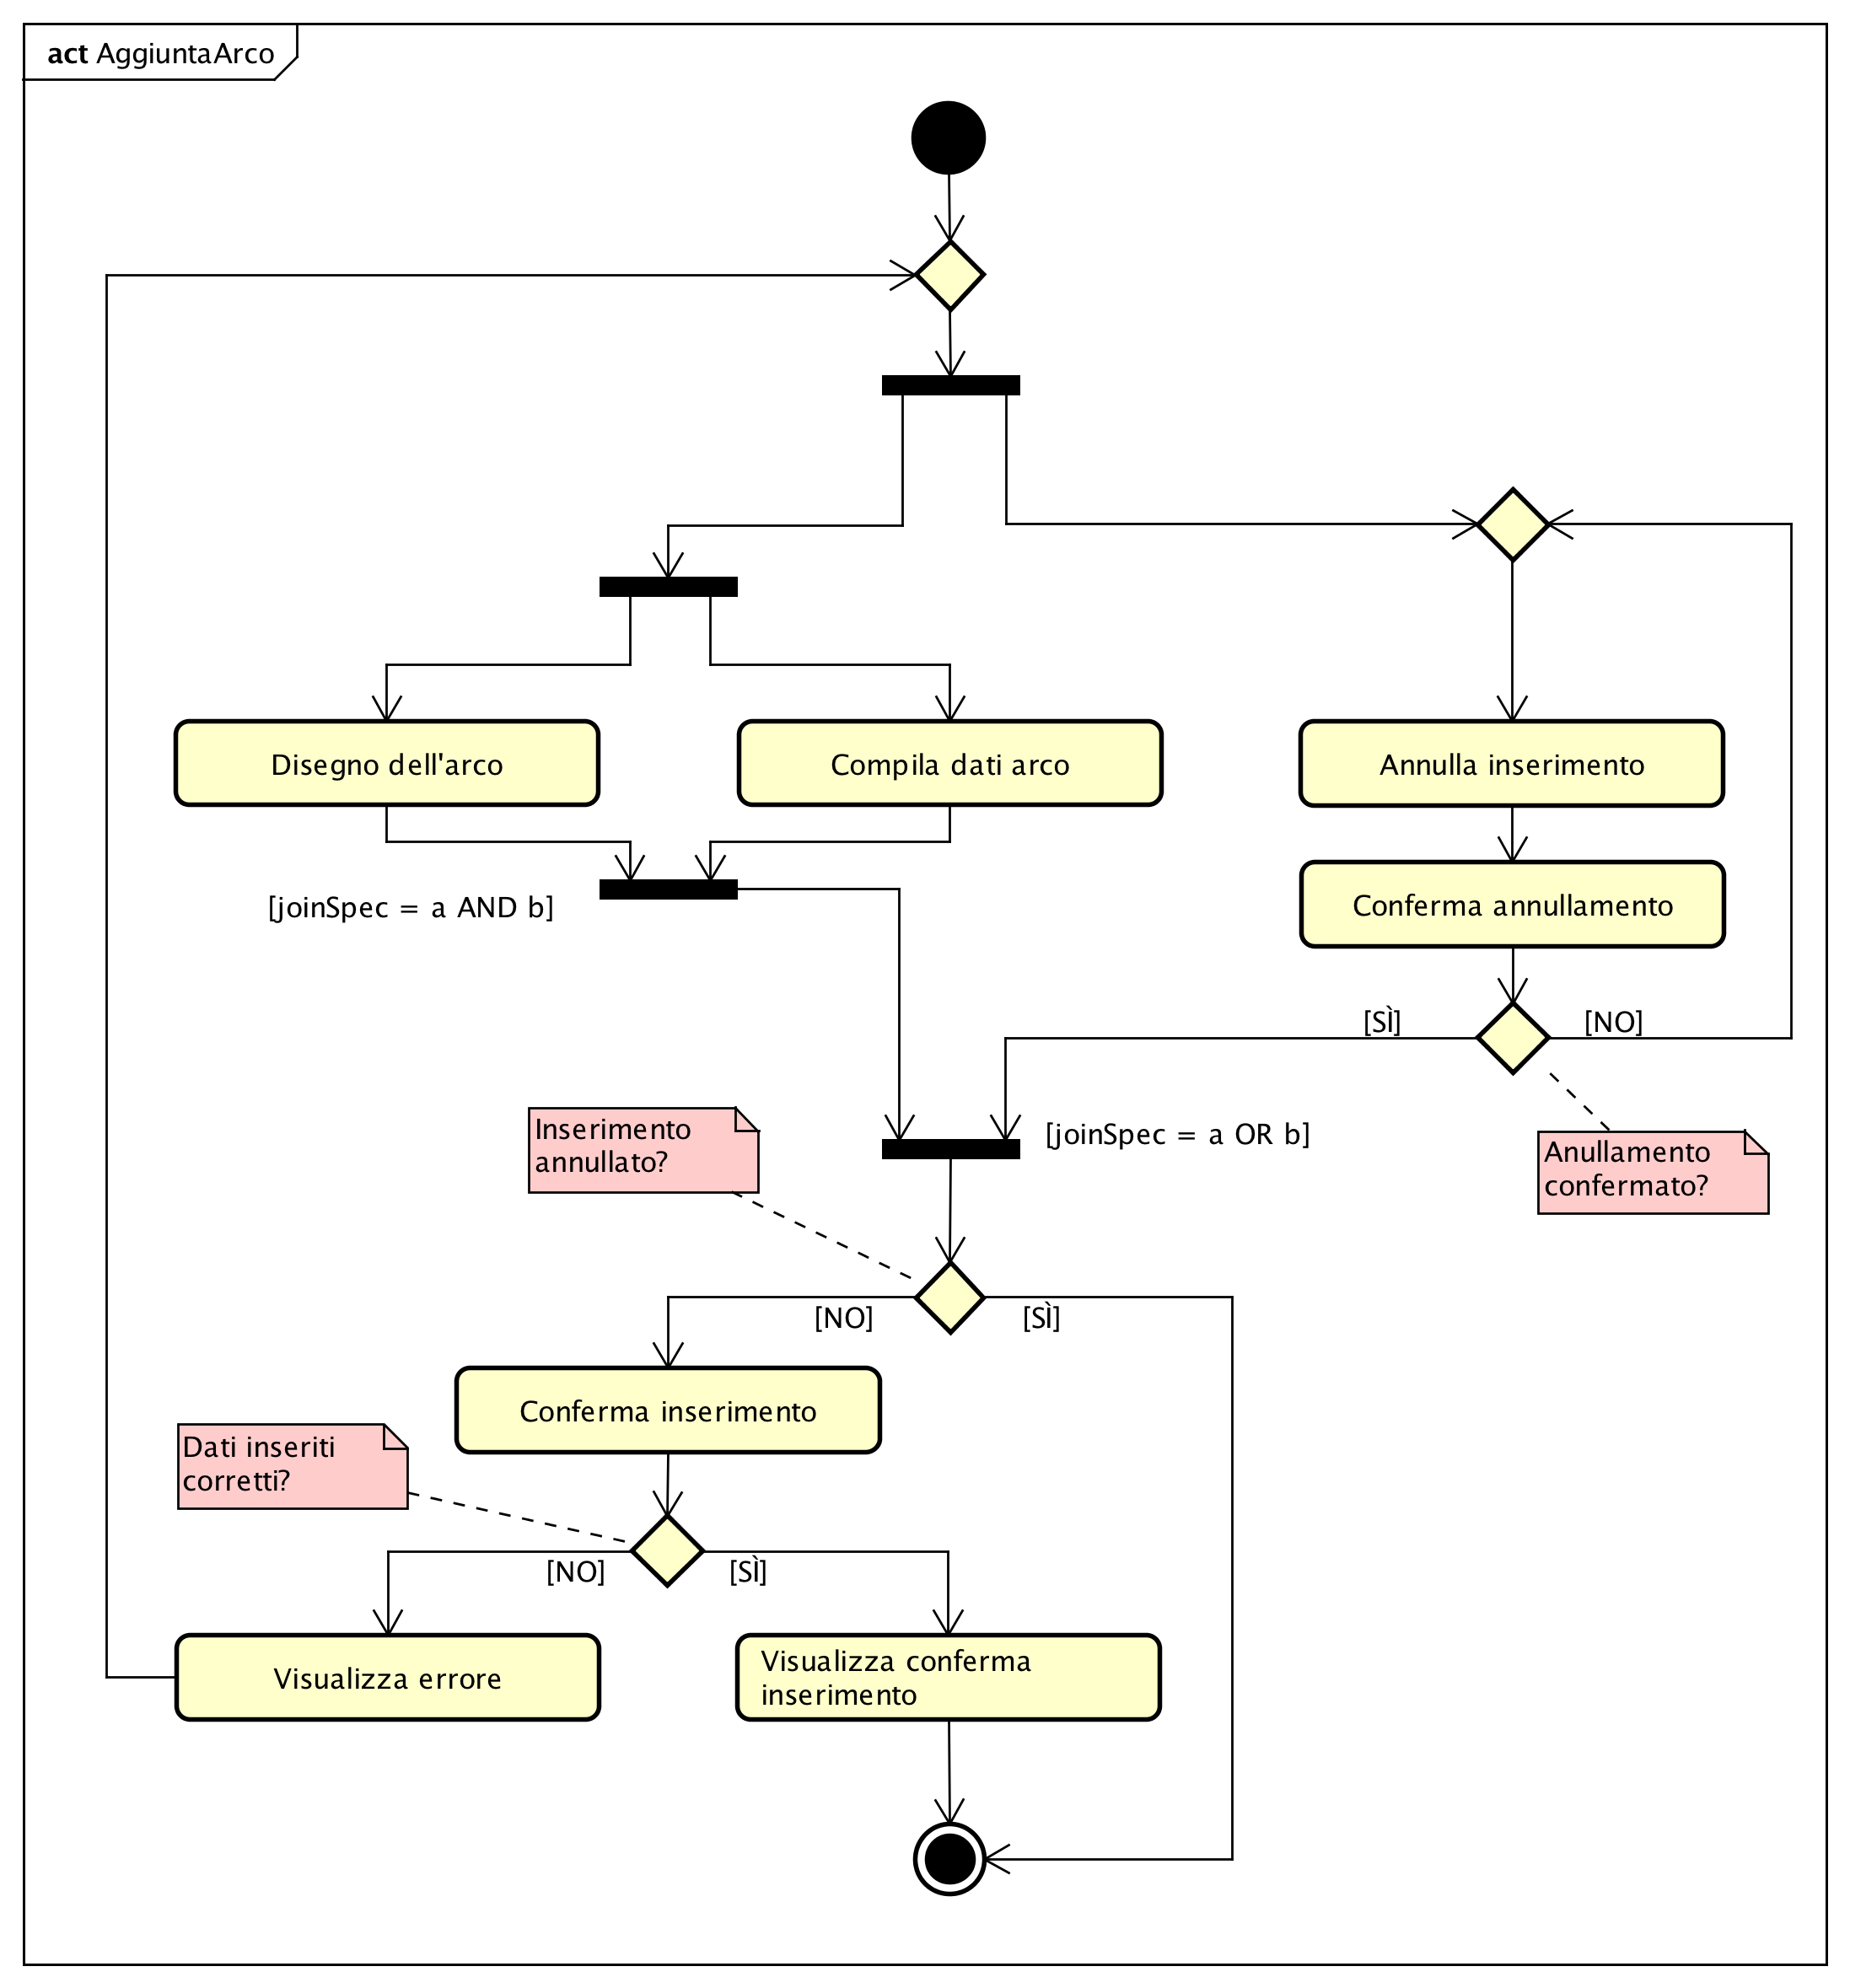
\includegraphics[width=\textwidth]{img/DiagrammiDiAttivita/AggiuntaArco.png}
	\caption{Diagramma di attività per l'aggiunta di un arco}
\end{figure}
\begin{figure}[H]
	\centering
	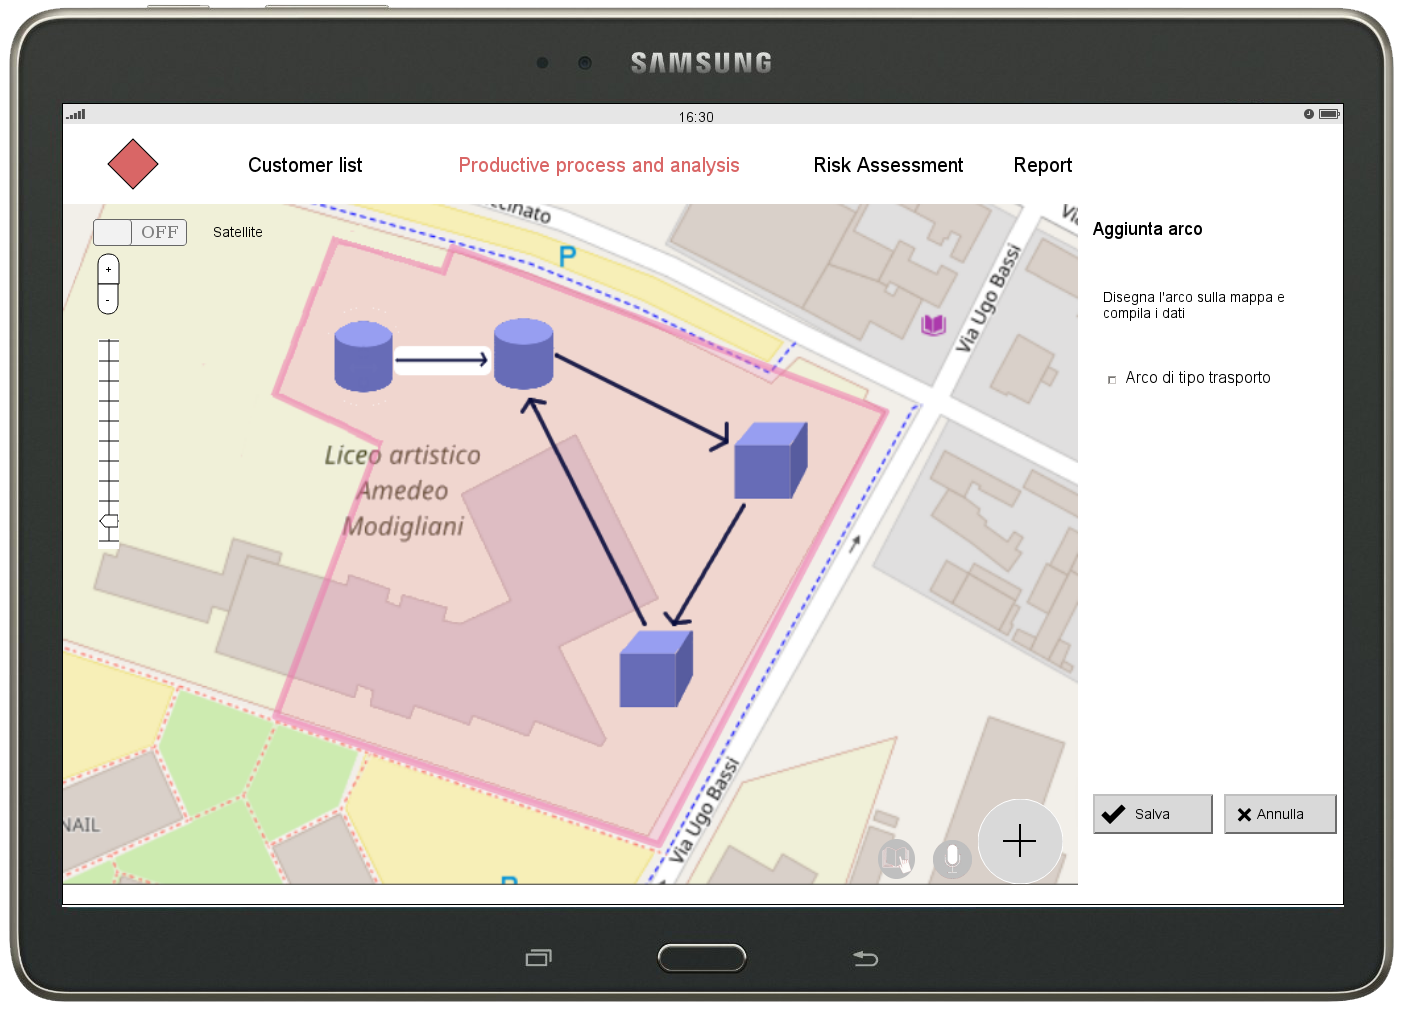
\includegraphics[width=\textwidth]{img/MockUp/m18.png}
	\caption{Mockup per l'aggiunta di un arco}
\end{figure}

\newpage
\subsection{Aggiunta scenario}
Per aggiungere uno scenario l'utente dovrà disegnare il perimetro dello scenario sulla mappa, compilarne i dati e confermare l'inserimento. In caso di dati non corretti, l'inserimento potrebbe non andare a buon fine: verrà visualizzato un messaggio di errore e l'utente sarà tenuto a correggere eventuali errori o incompletezze.
In ogni momento l'utente può annullare l'inserimento. Il sistema richiede una conferma per portare a termine tale operazione.
\begin{figure}[H]
	\centering
	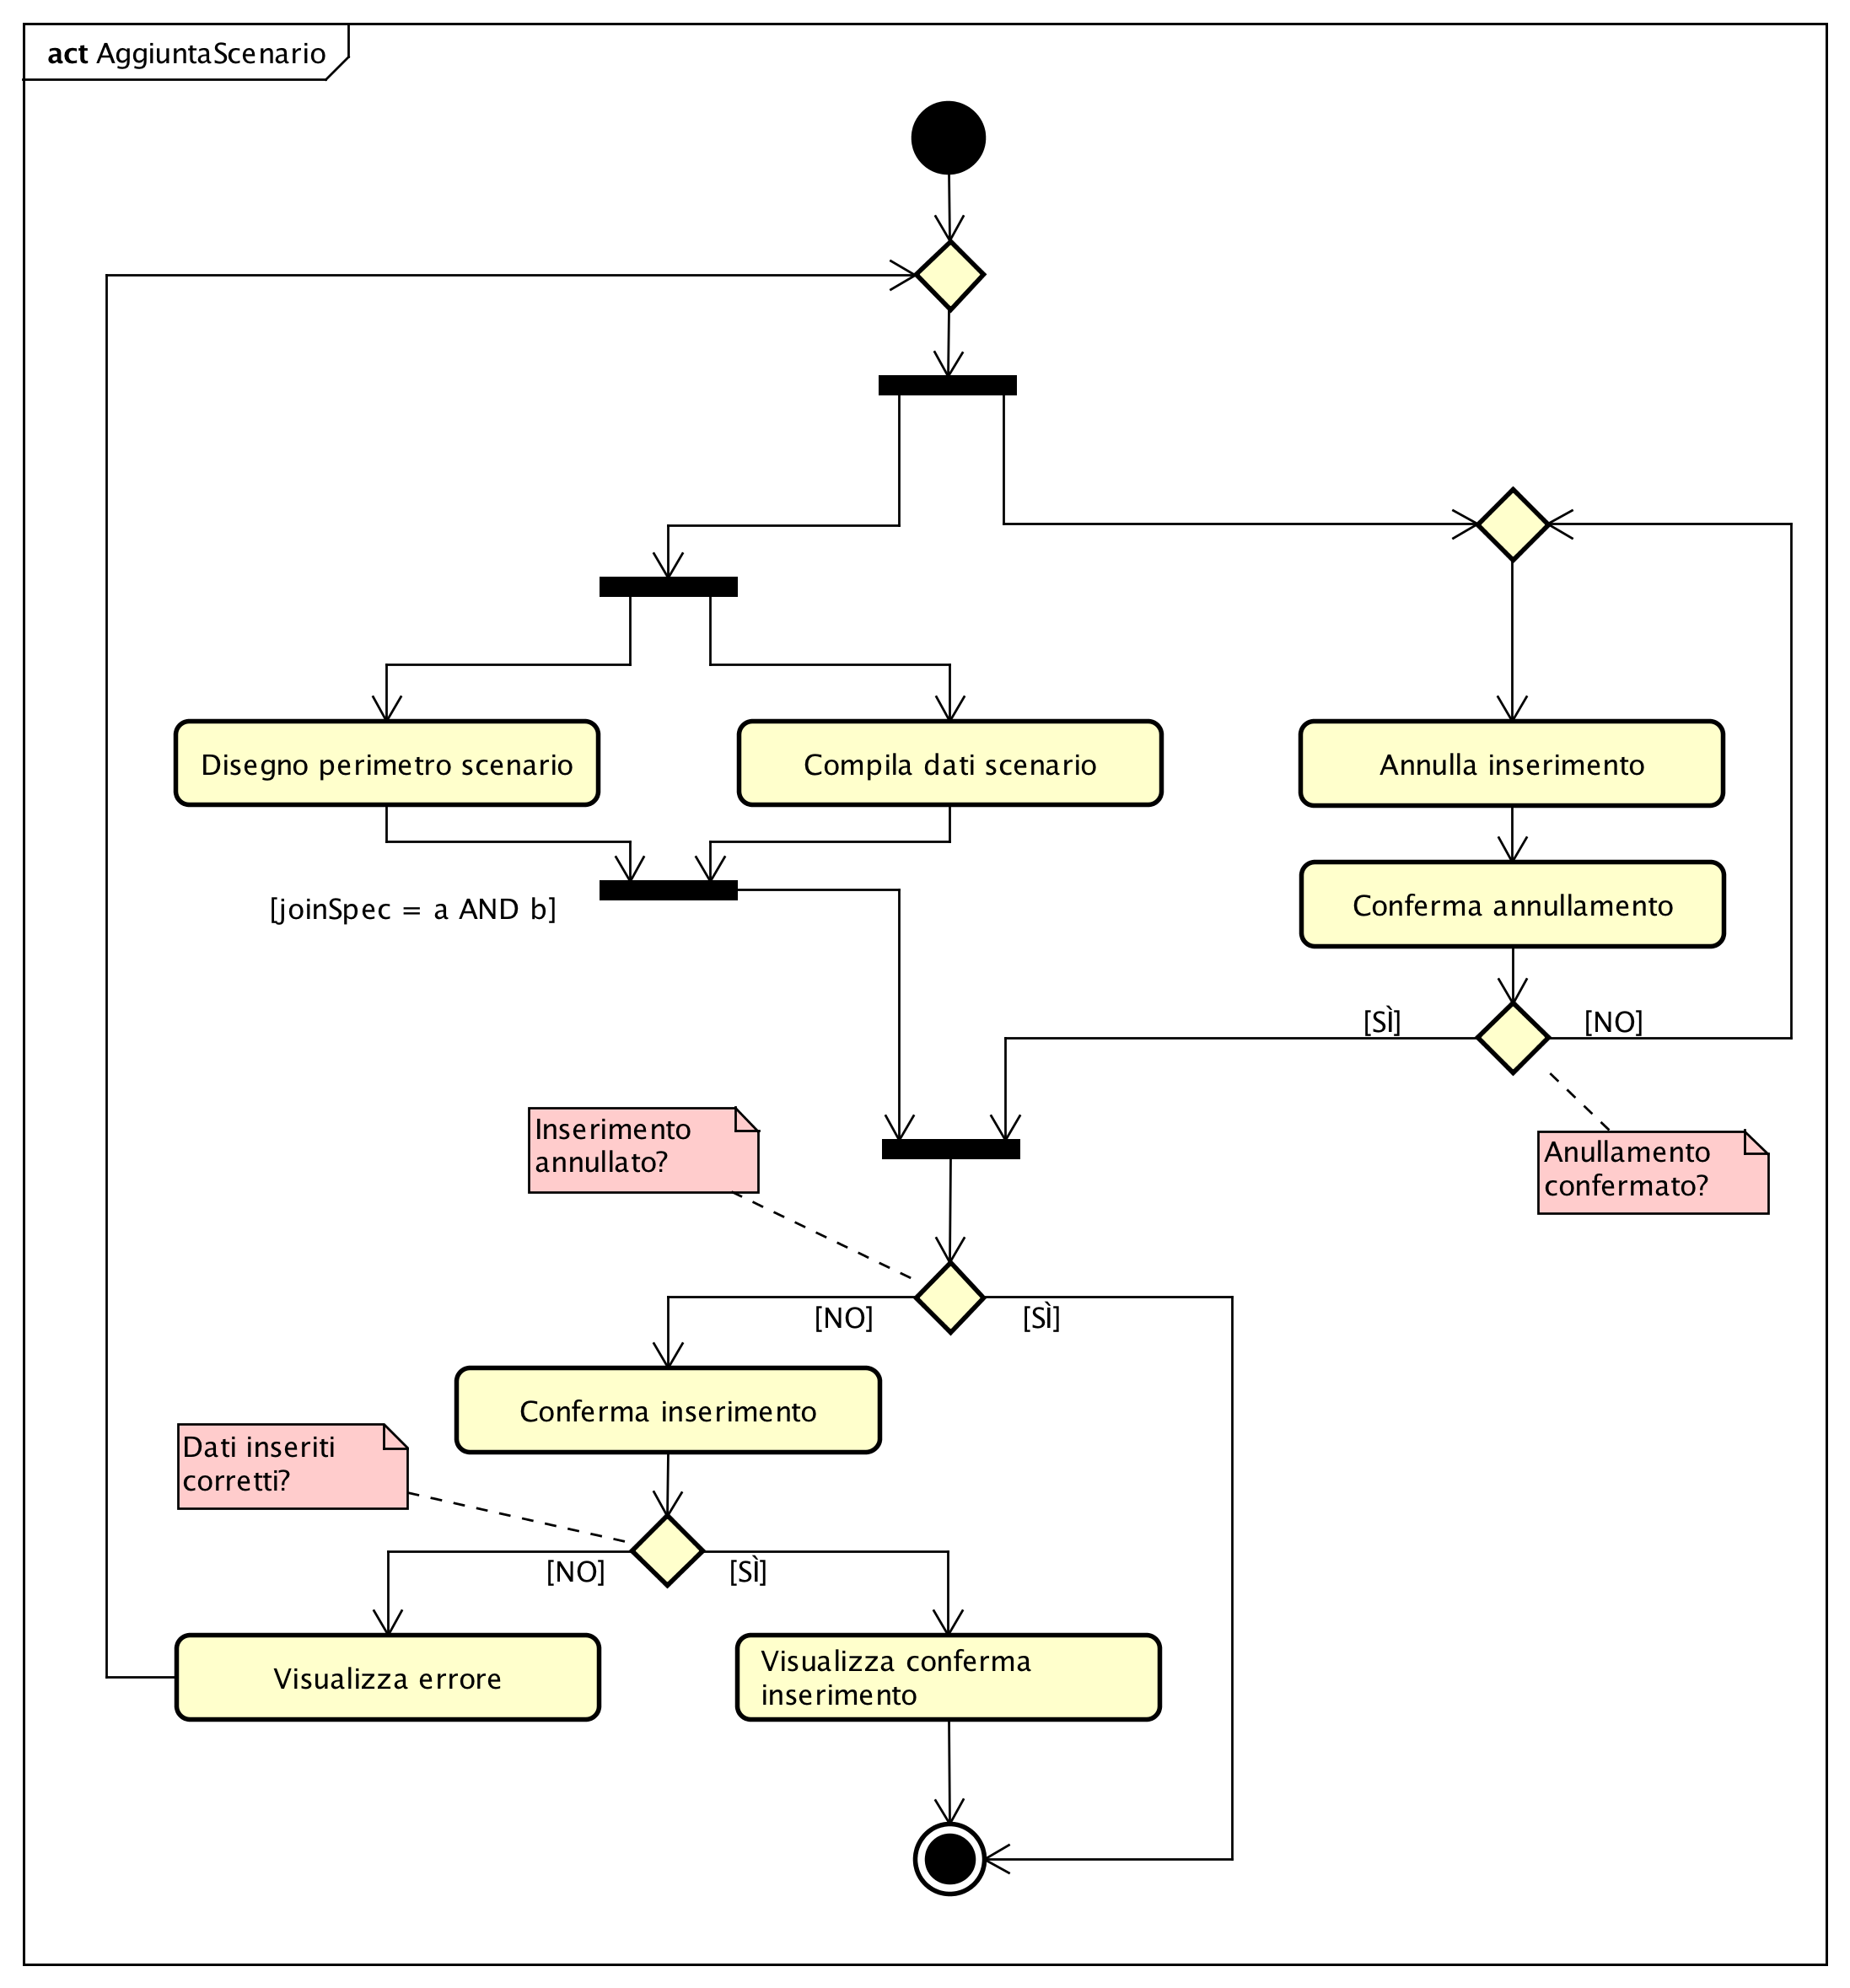
\includegraphics[width=\textwidth]{img/DiagrammiDiAttivita/AggiuntaScenario.png}
	\caption{Diagramma di attività per l'aggiunta di uno scenario}
\end{figure}
\begin{figure}[H]
	\centering
	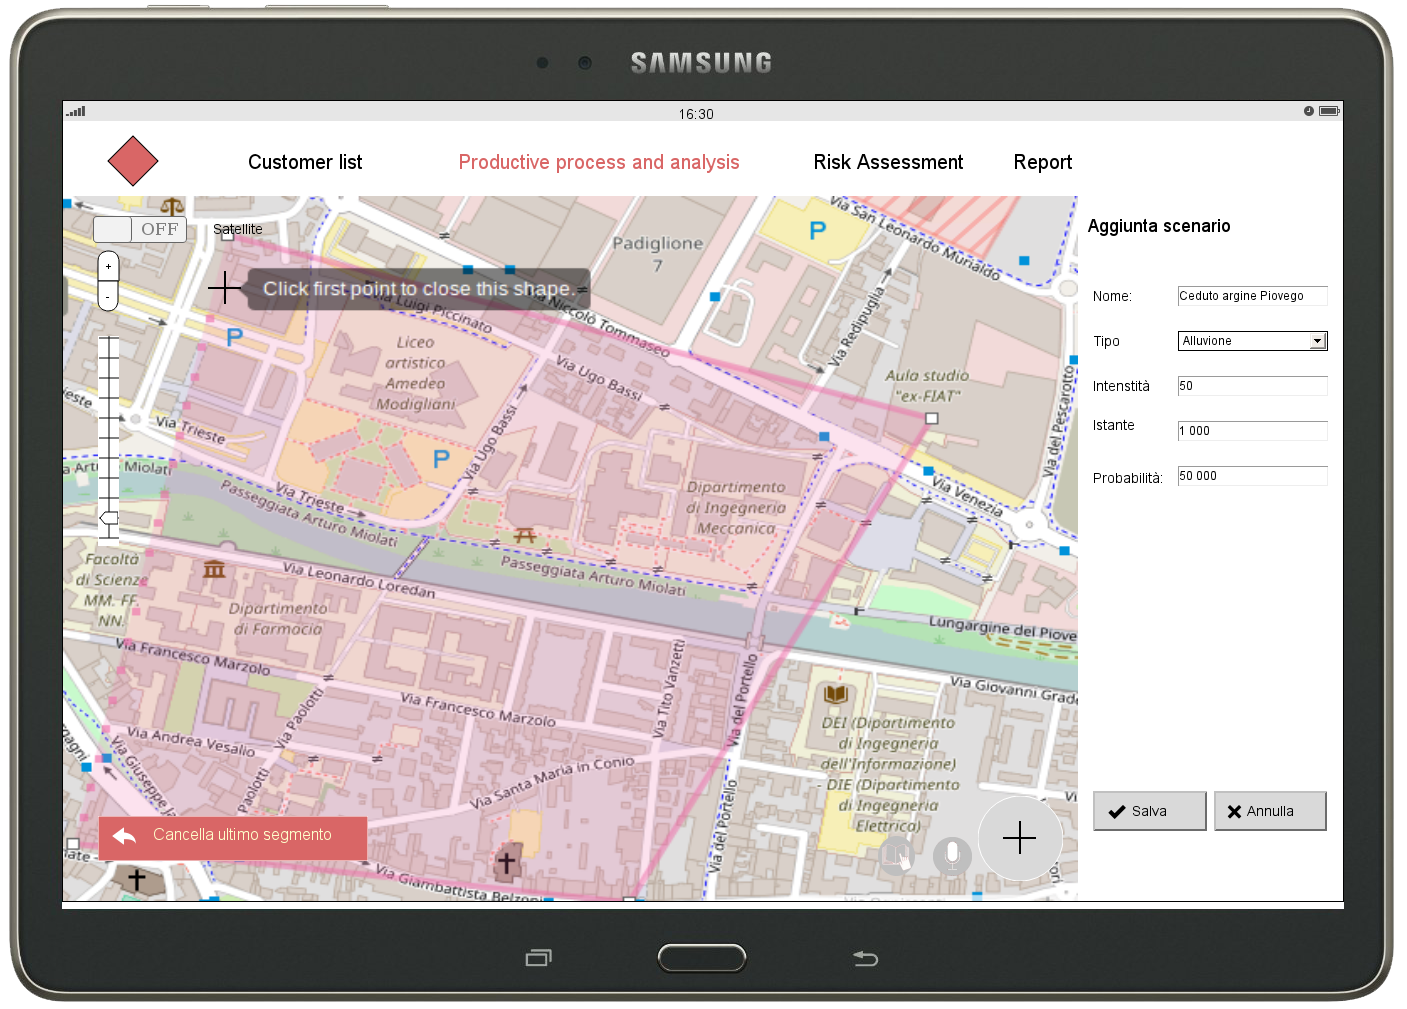
\includegraphics[width=\textwidth]{img/MockUp/m20.png}
	\caption{Mockup per l'aggiunta di uno scenario}
\end{figure}

\newpage
\subsection{Gestione Analisi}
Dopo essere entrati nella sezione di analisi, l'utente può effettuare ripetutamente una tra le seguenti operazioni:
\begin{itemize}
	\item è possibile aggiungere scenari su cui non è ancora stata calcolata alla lista di quelli da analizzare. In seguito è possibile avviare l'analisi;
	\item è possibile eliminare scenari dalla lista degli scenari su cui è stata calcolata l'analisi. In questo caso l'utente è invitato a confermare l'eliminazione o ad annullarla;
	\item l'utente non può effettuare alcuna operazione all'interno della sezione di analisi, se non sono presenti scenari.
\end{itemize} 
\begin{figure}[H]
	\centering
	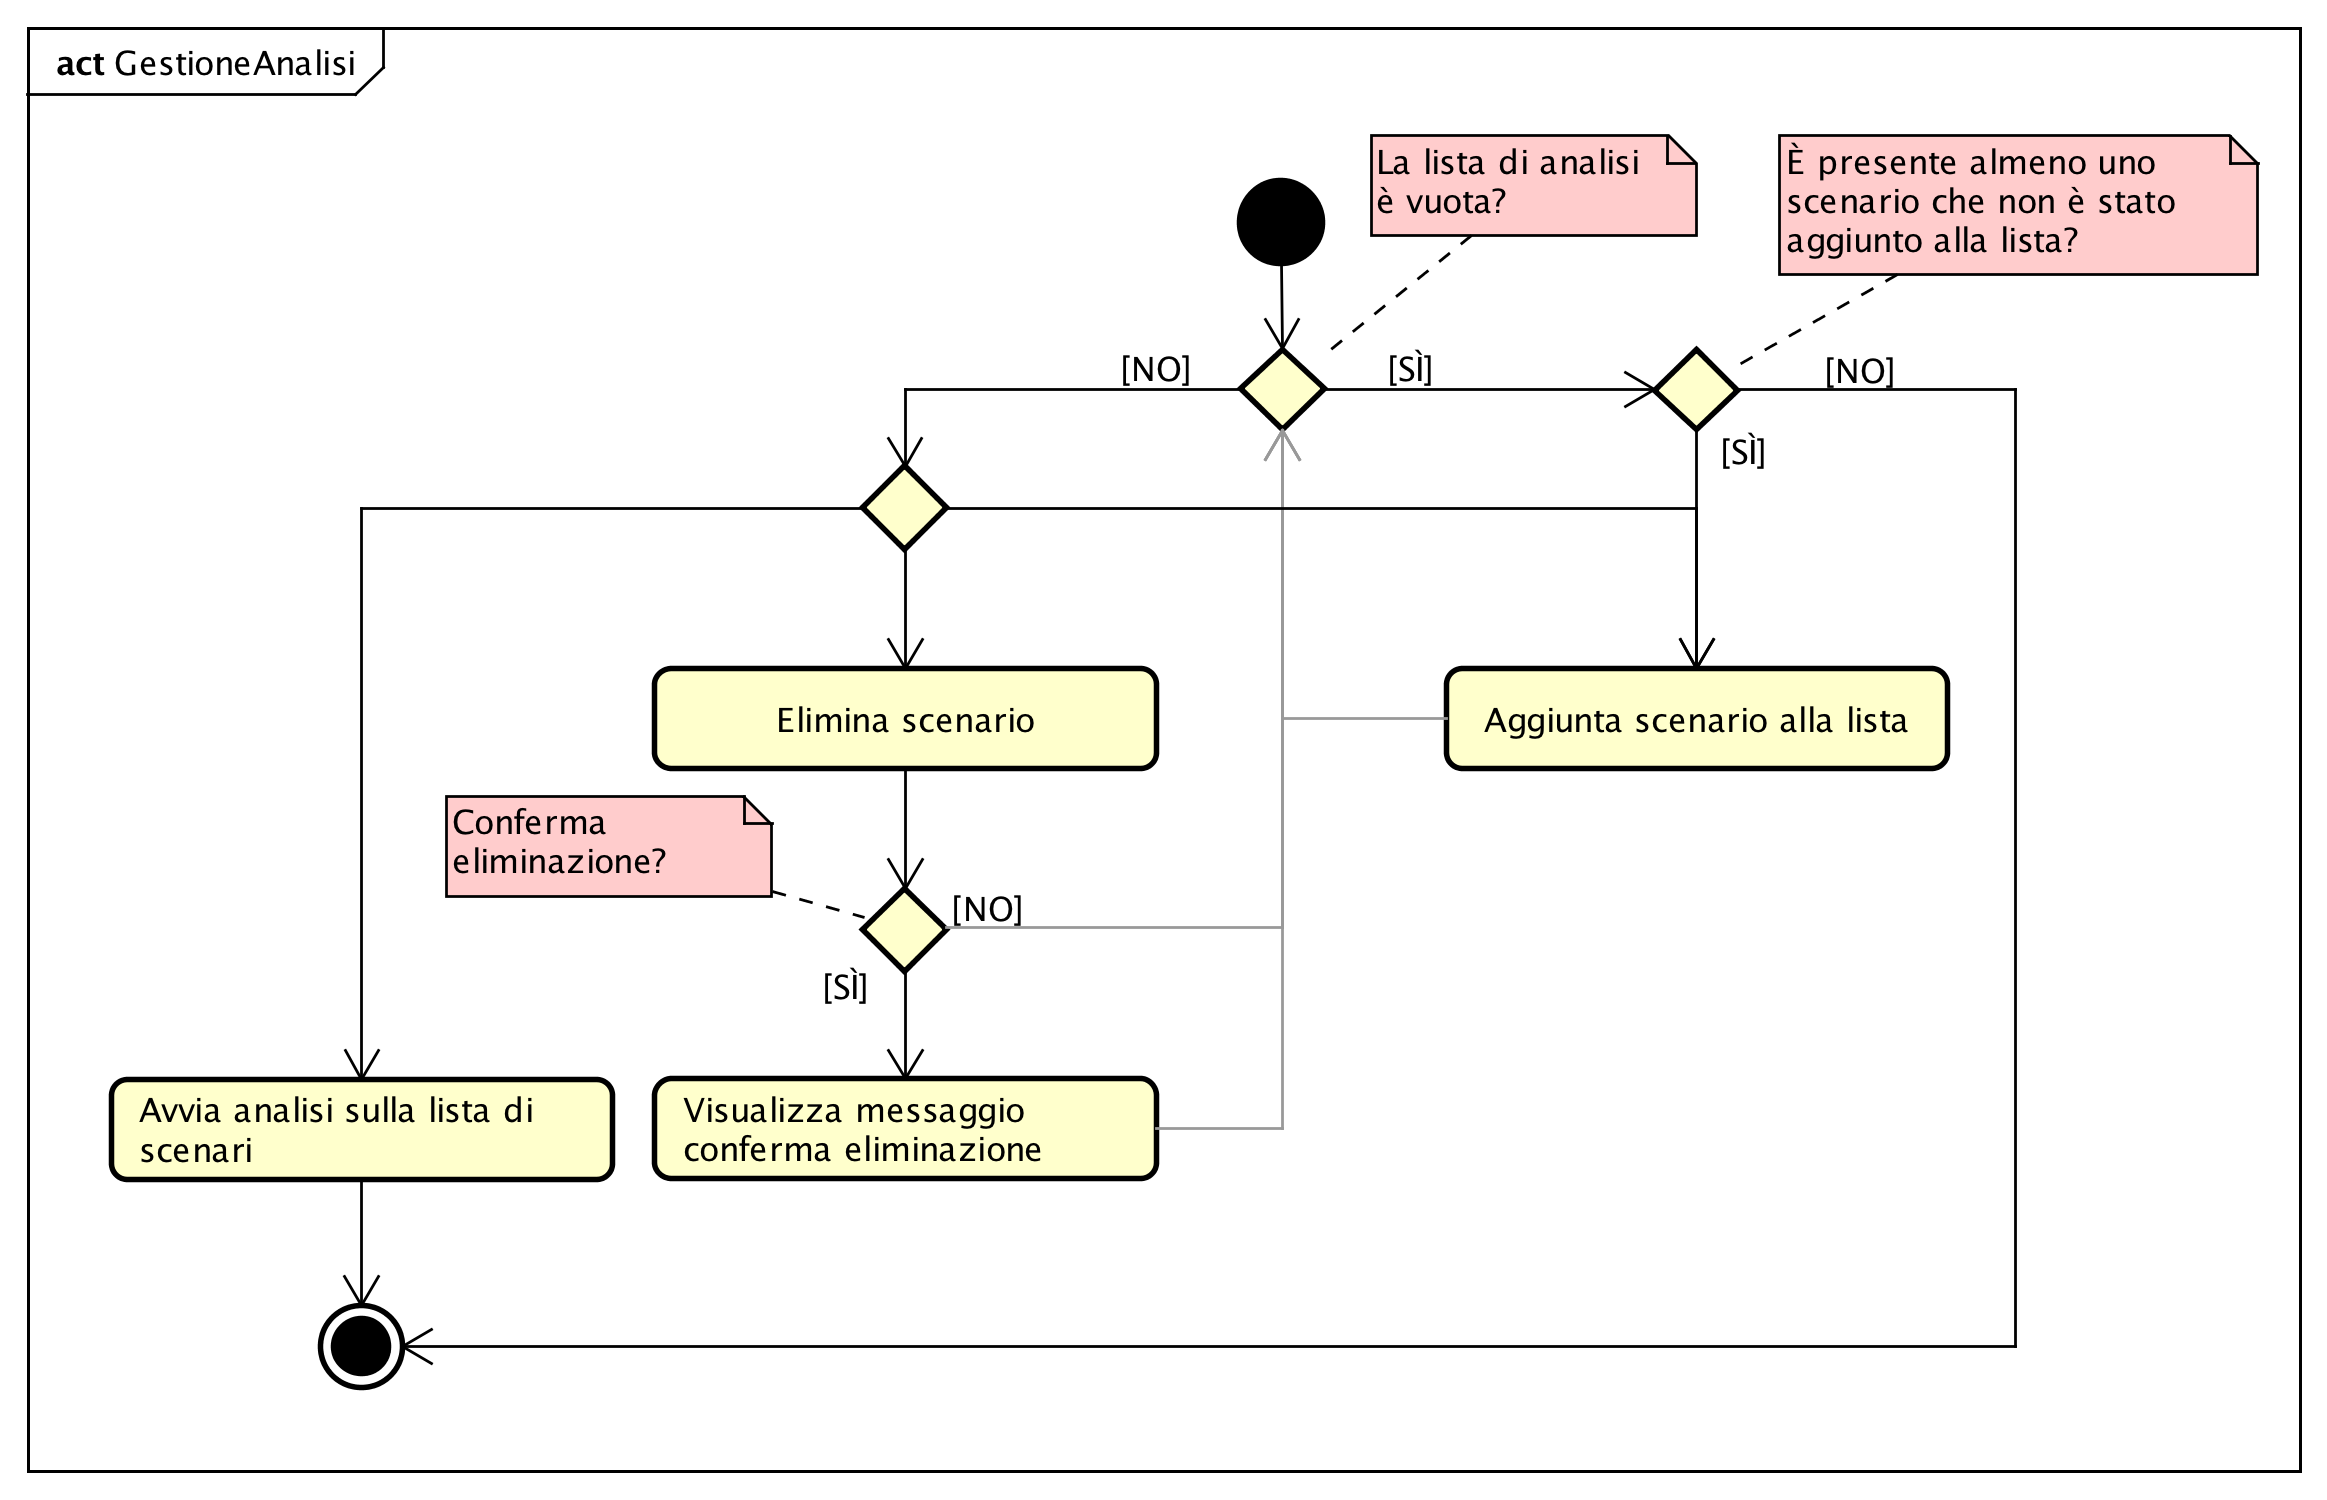
\includegraphics[width=\textwidth]{img/DiagrammiDiAttivita/GestioneAnalisi.png}
	\caption{Diagramma di attività per la gestione analisi}
\end{figure}
\begin{figure}[H]
	\centering
	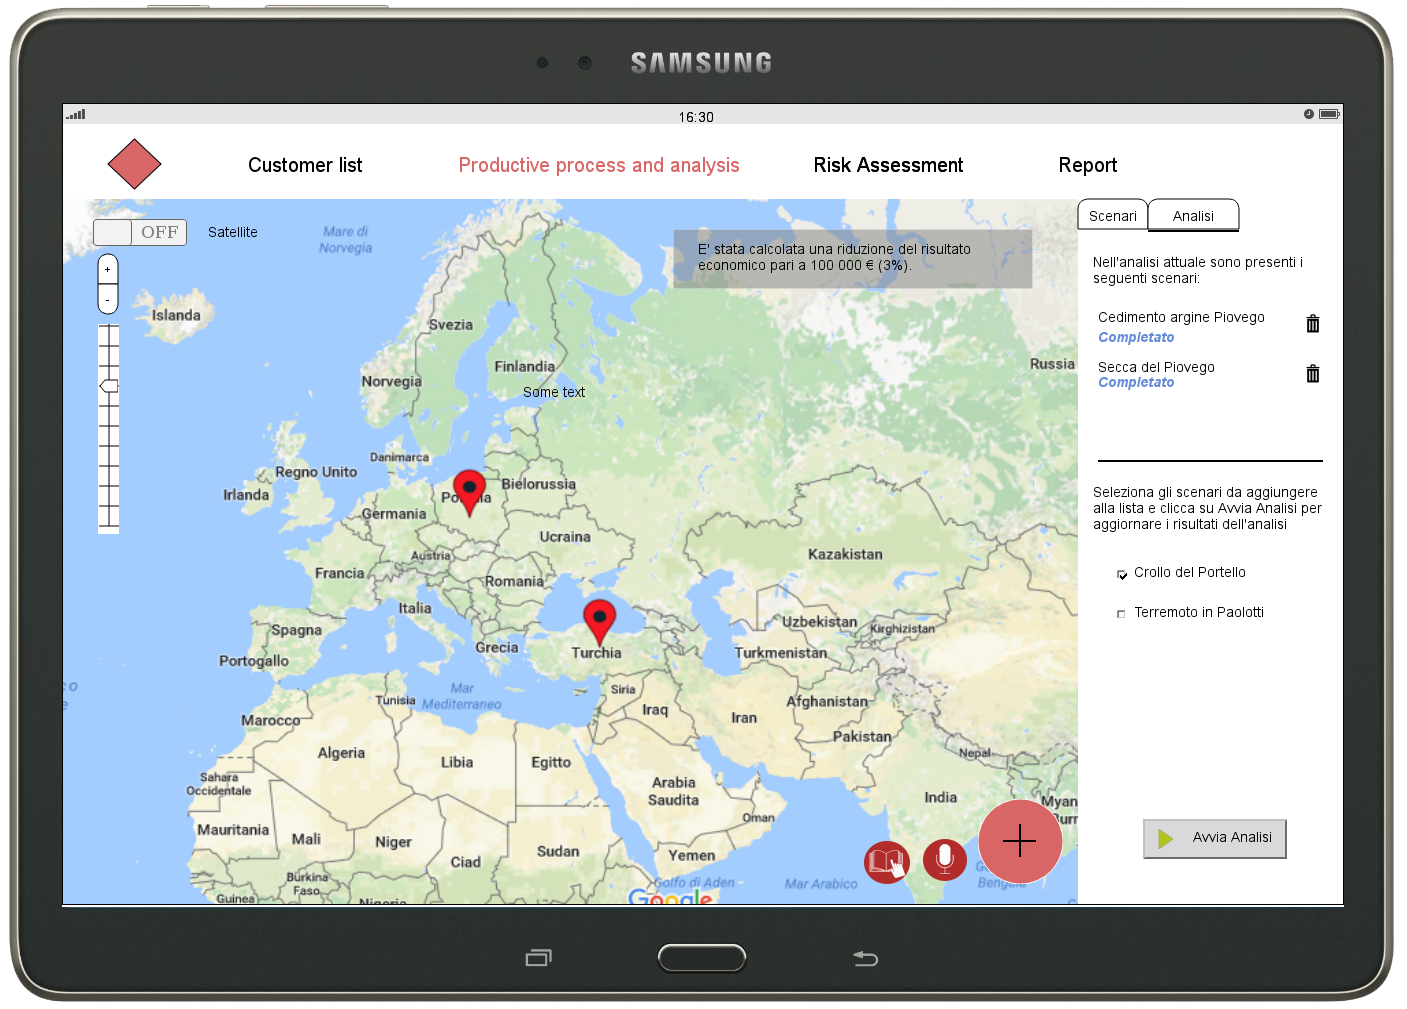
\includegraphics[scale=0.29]{img/MockUp/m2.png}
	\caption{Mockup per l'avvio dell'analisi}
\end{figure}
\begin{figure}[H]
	\centering
	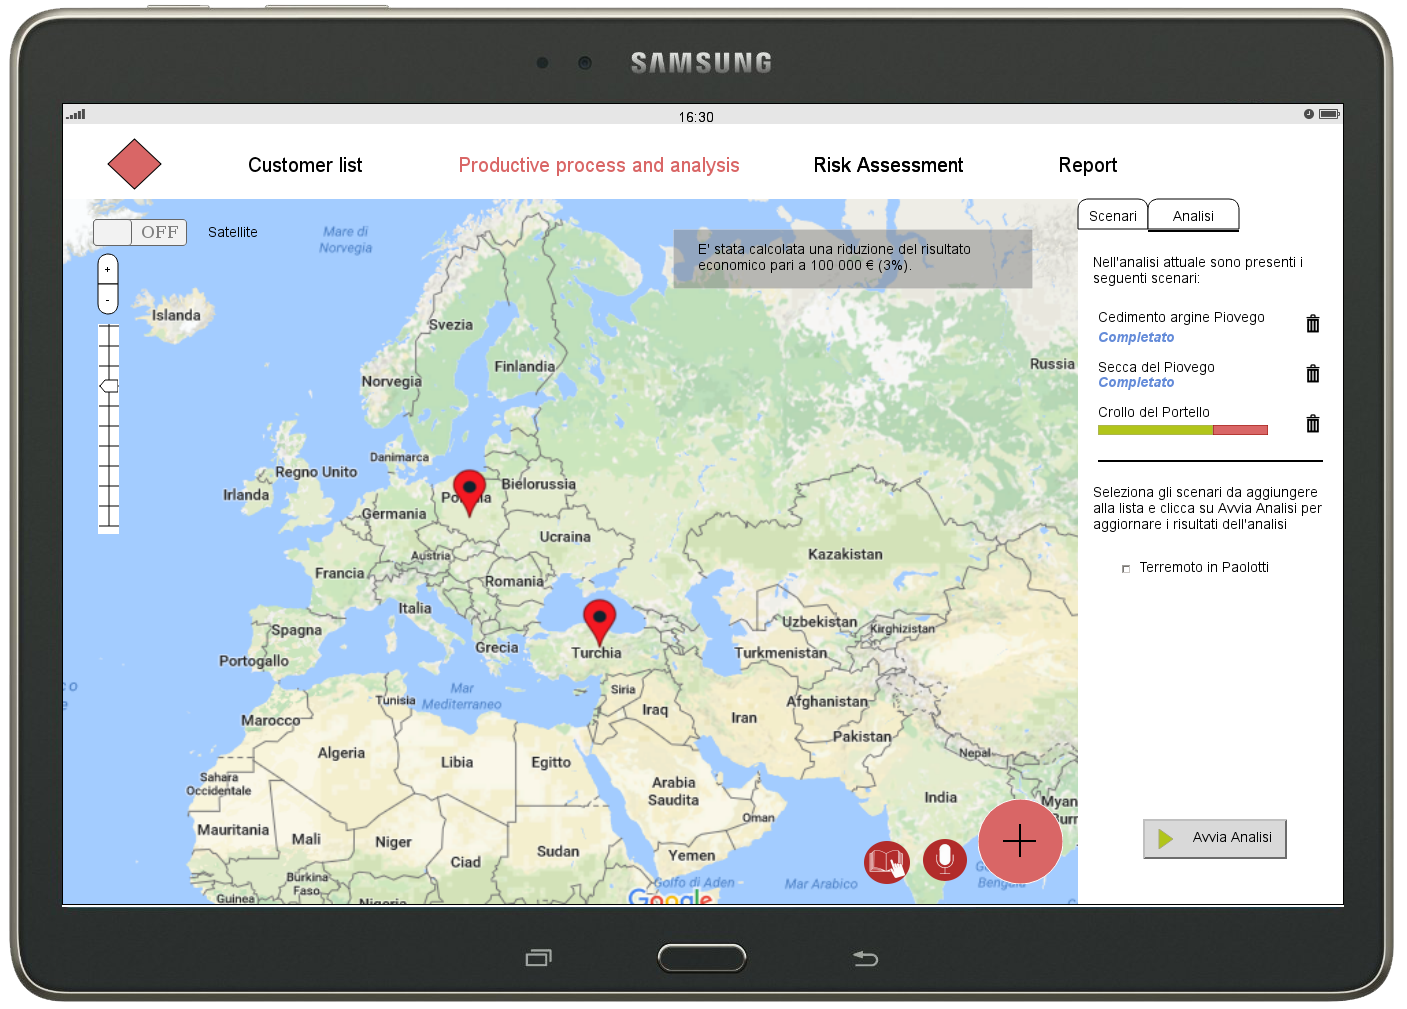
\includegraphics[scale=0.29]{img/MockUp/m3.png}
	\caption{Mockup per l'analisi in corso}
\end{figure}


\newpage
\subsection{Selezione asset}
Una volta selezionato l'asset l'utente potrà:
\begin{itemize}
	\item centrarlo automaticamente sulla mappa (utile nel caso in cui nel frattempo l'utente si sia spostato sulla mappa), eventualmente più volte, senza annullarne la selezione;
	\item annullarne la selezione;
	\item modificarlo;
	\item eliminarlo.
\end{itemize}
\begin{figure}[H]
	\centering
	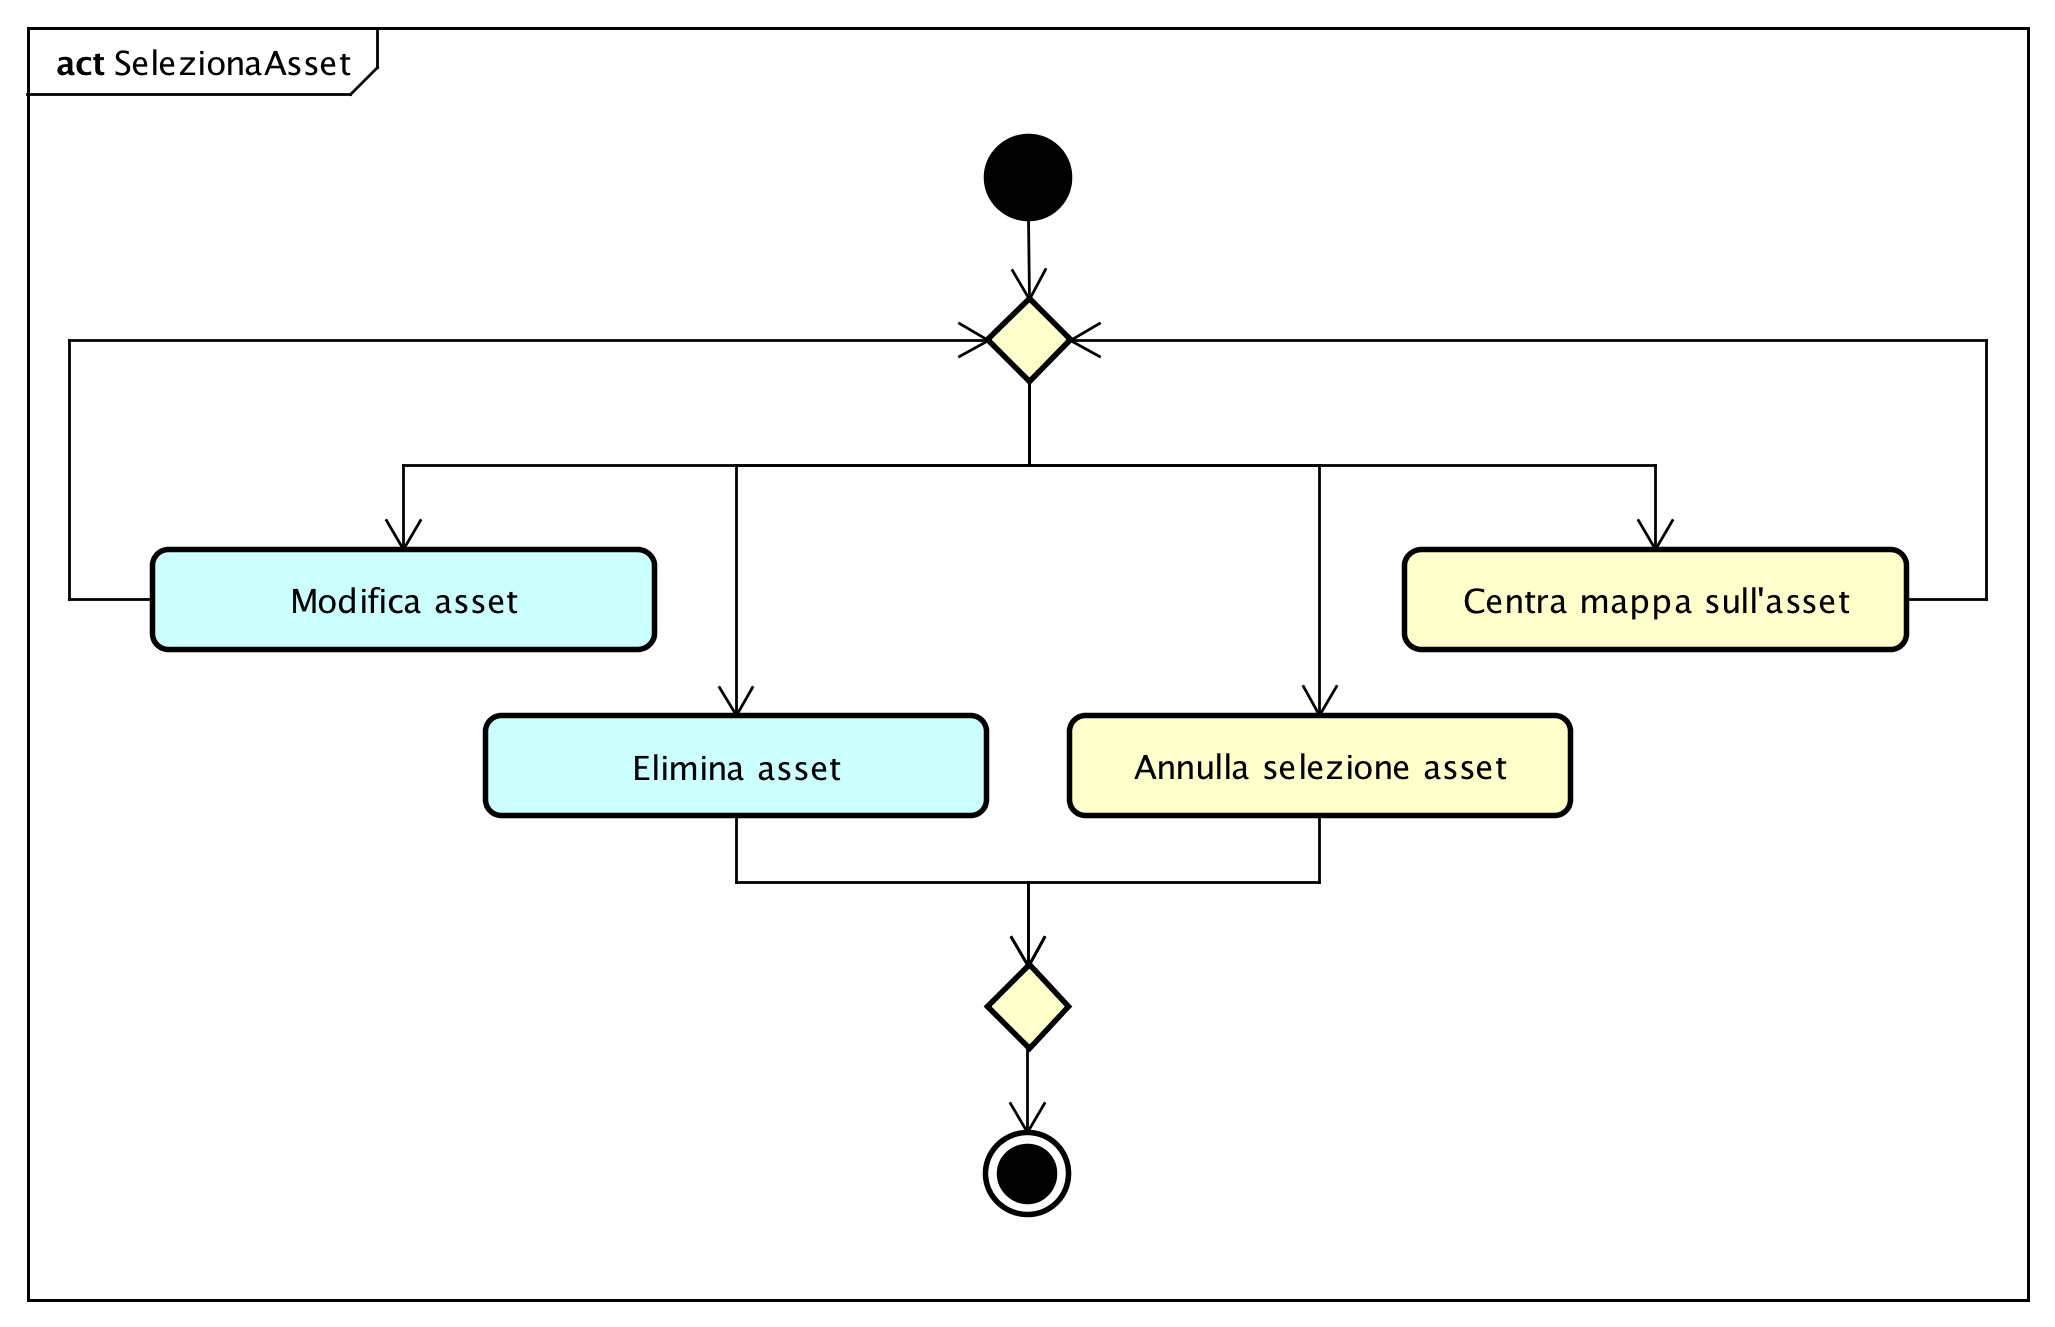
\includegraphics[width=\textwidth]{img/DiagrammiDiAttivita/SelezioneAsset.png}
	\caption{Diagramma di attività per la selezione di un asset}
\end{figure}
\label{7_Visualizza_un_asset}
\begin{figure}[H]
	\centering
	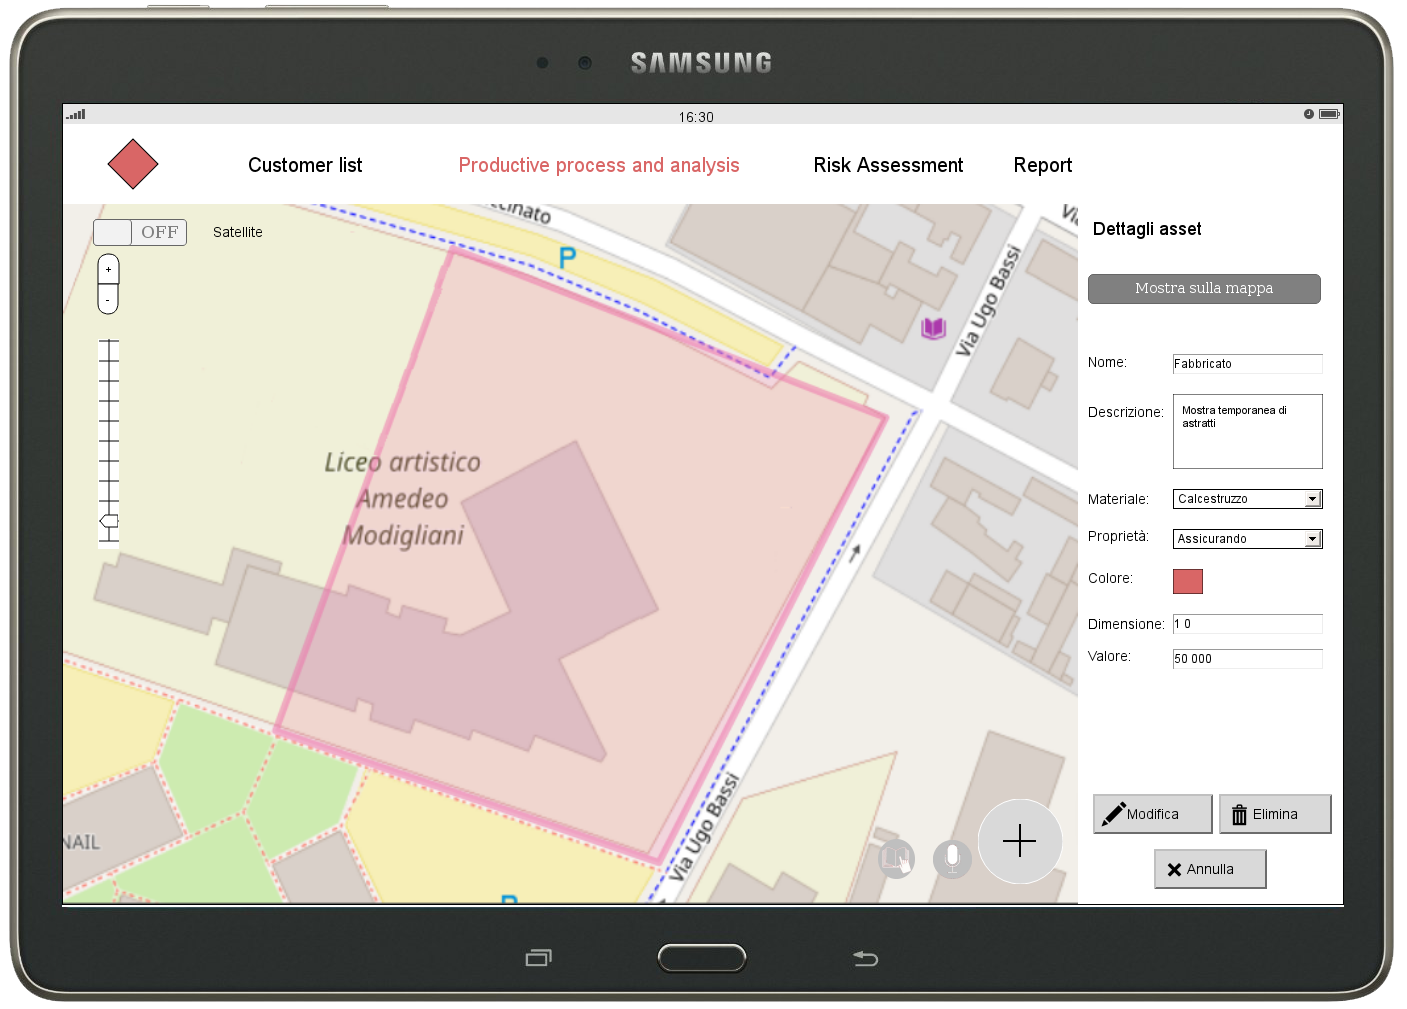
\includegraphics[width=\textwidth]{img/MockUp/m7.png}
	\caption{Mockup per la selezione di un asset}
\end{figure}

\newpage
\subsection{Selezione nodo}
Una volta selezionato il nodo l'utente potrà:
\begin{itemize}
	\item centrarlo automaticamente sulla mappa (utile nel caso in cui nel frattempo l'utente si sia spostato sulla mappa), eventualmente più volte, senza annullarne la selezione;
	\item annullarne la selezione;
	\item modificarlo;
	\item eliminarlo.
\end{itemize}
\begin{figure}[H]
	\centering
	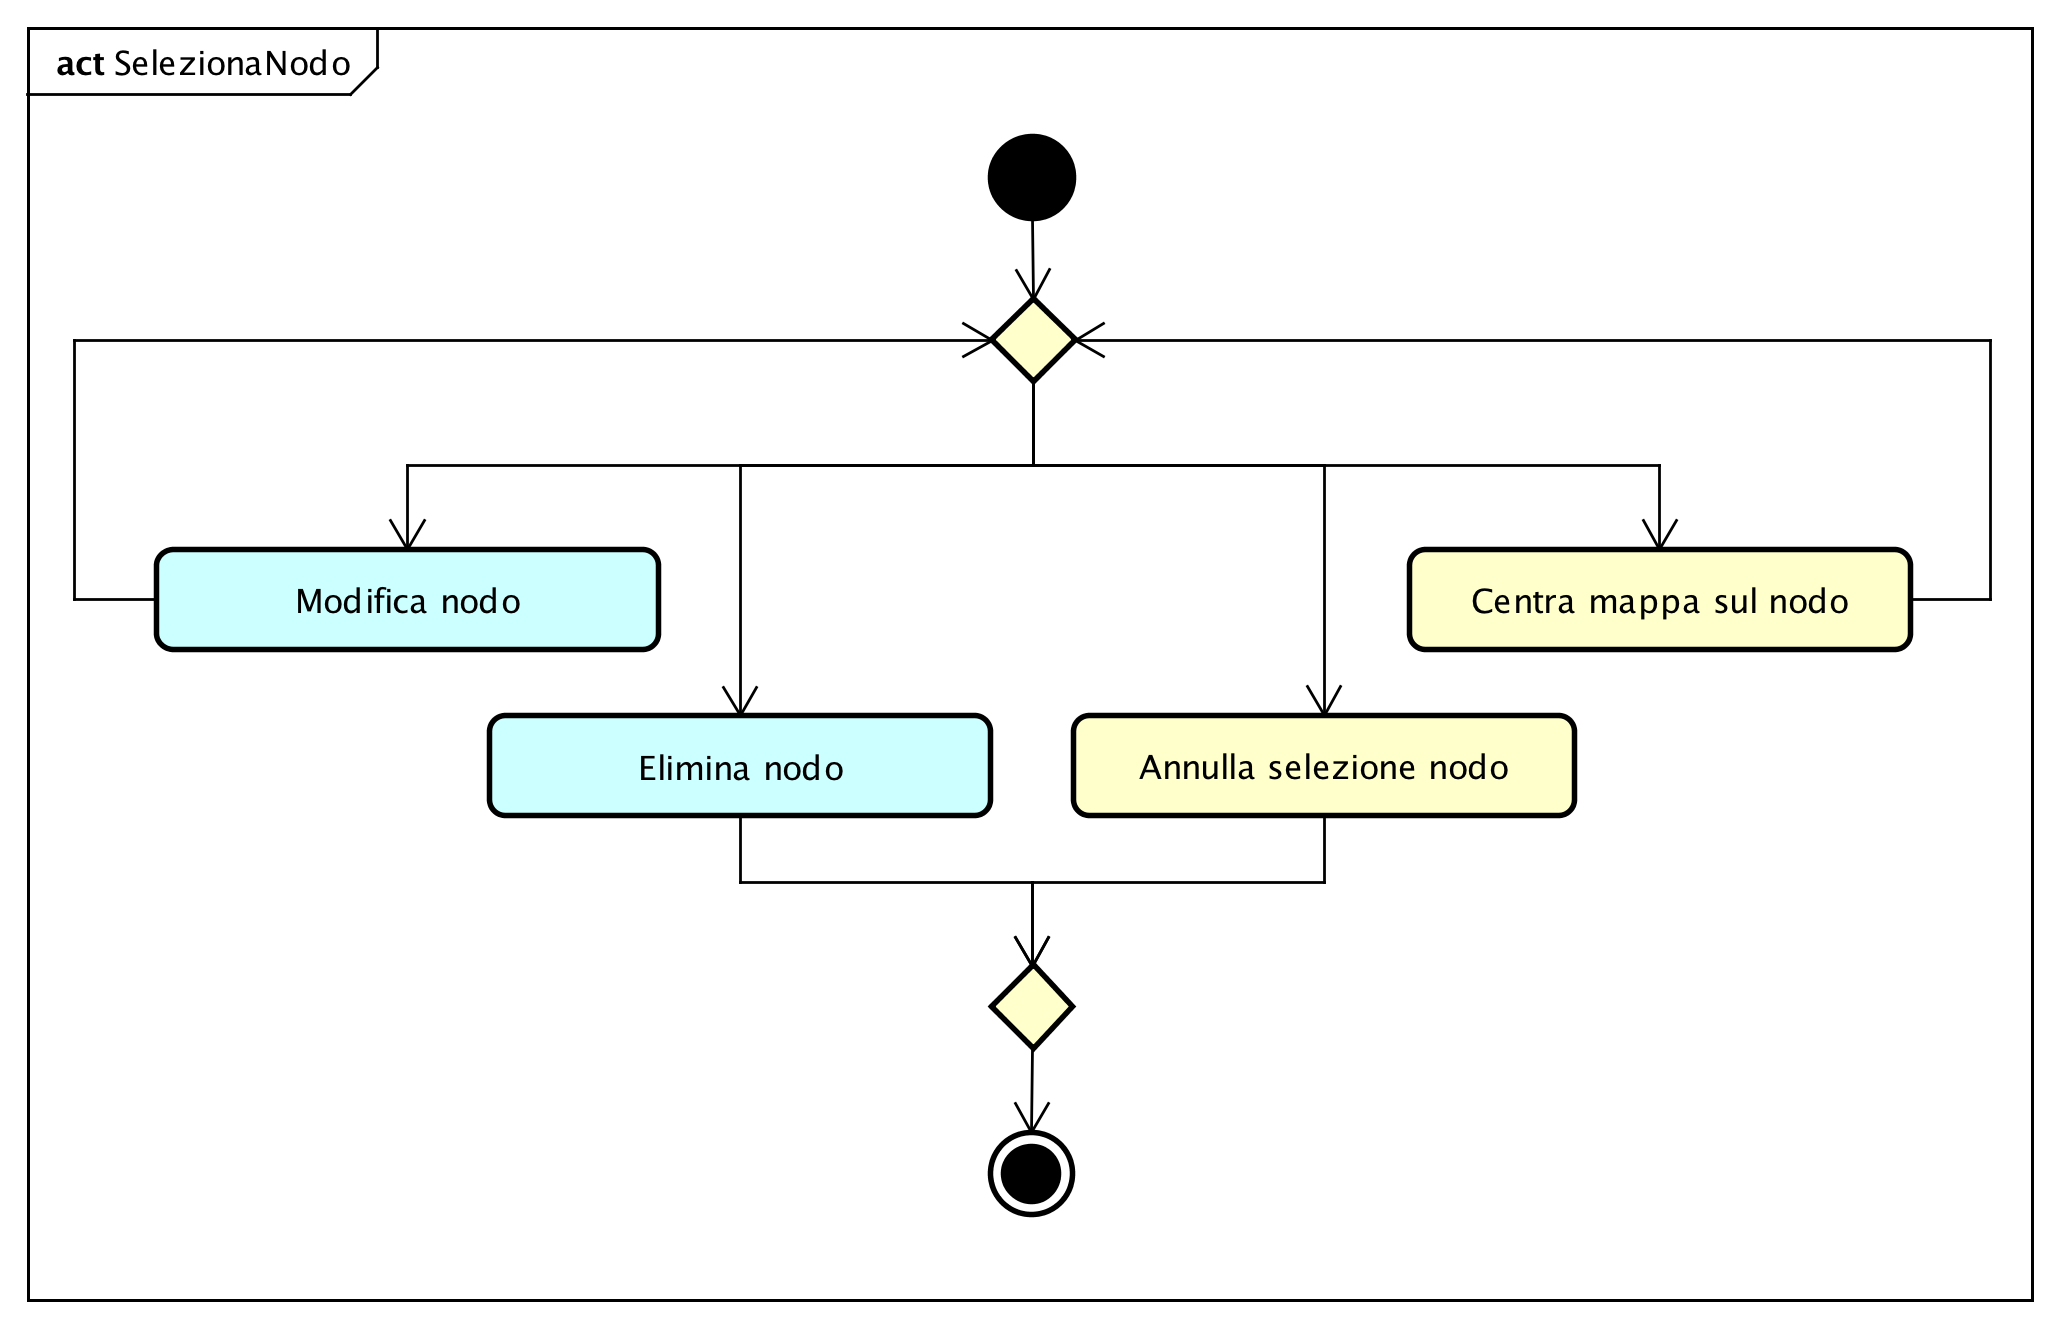
\includegraphics[width=\textwidth]{img/DiagrammiDiAttivita/SelezioneNodo.png}
	\caption{Diagramma di attività per la selezione di un nodo}
\end{figure}
\begin{figure}[H]
	\centering
	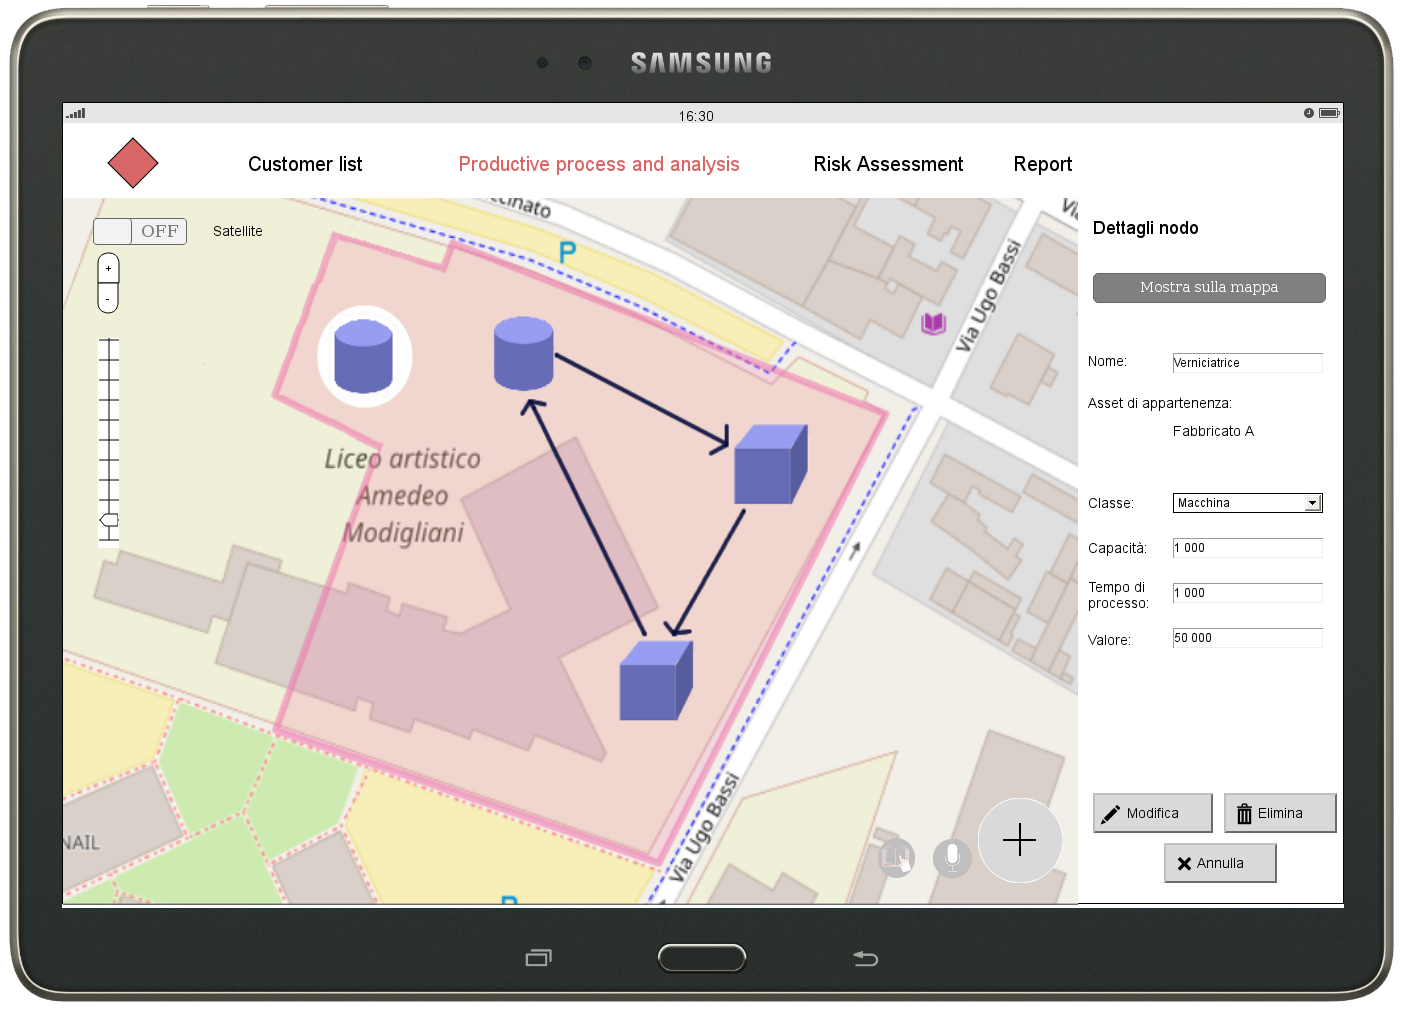
\includegraphics[width=\textwidth]{img/MockUp/m13.png}
	\caption{Mockup per la selezione di un nodo}
\end{figure}

\newpage
\subsection{Selezione arco}
Una volta selezionato il nodo l'utente potrà:
\begin{itemize}
	\item centrarlo automaticamente sulla mappa (utile nel caso in cui nel frattempo l'utente si sia spostato sulla mappa), eventualmente più volte, senza annullarne la selezione;
	\item annullarne la selezione;
	\item modificarlo;
	\item eliminarlo.
\end{itemize}
\begin{figure}[H]
	\centering
	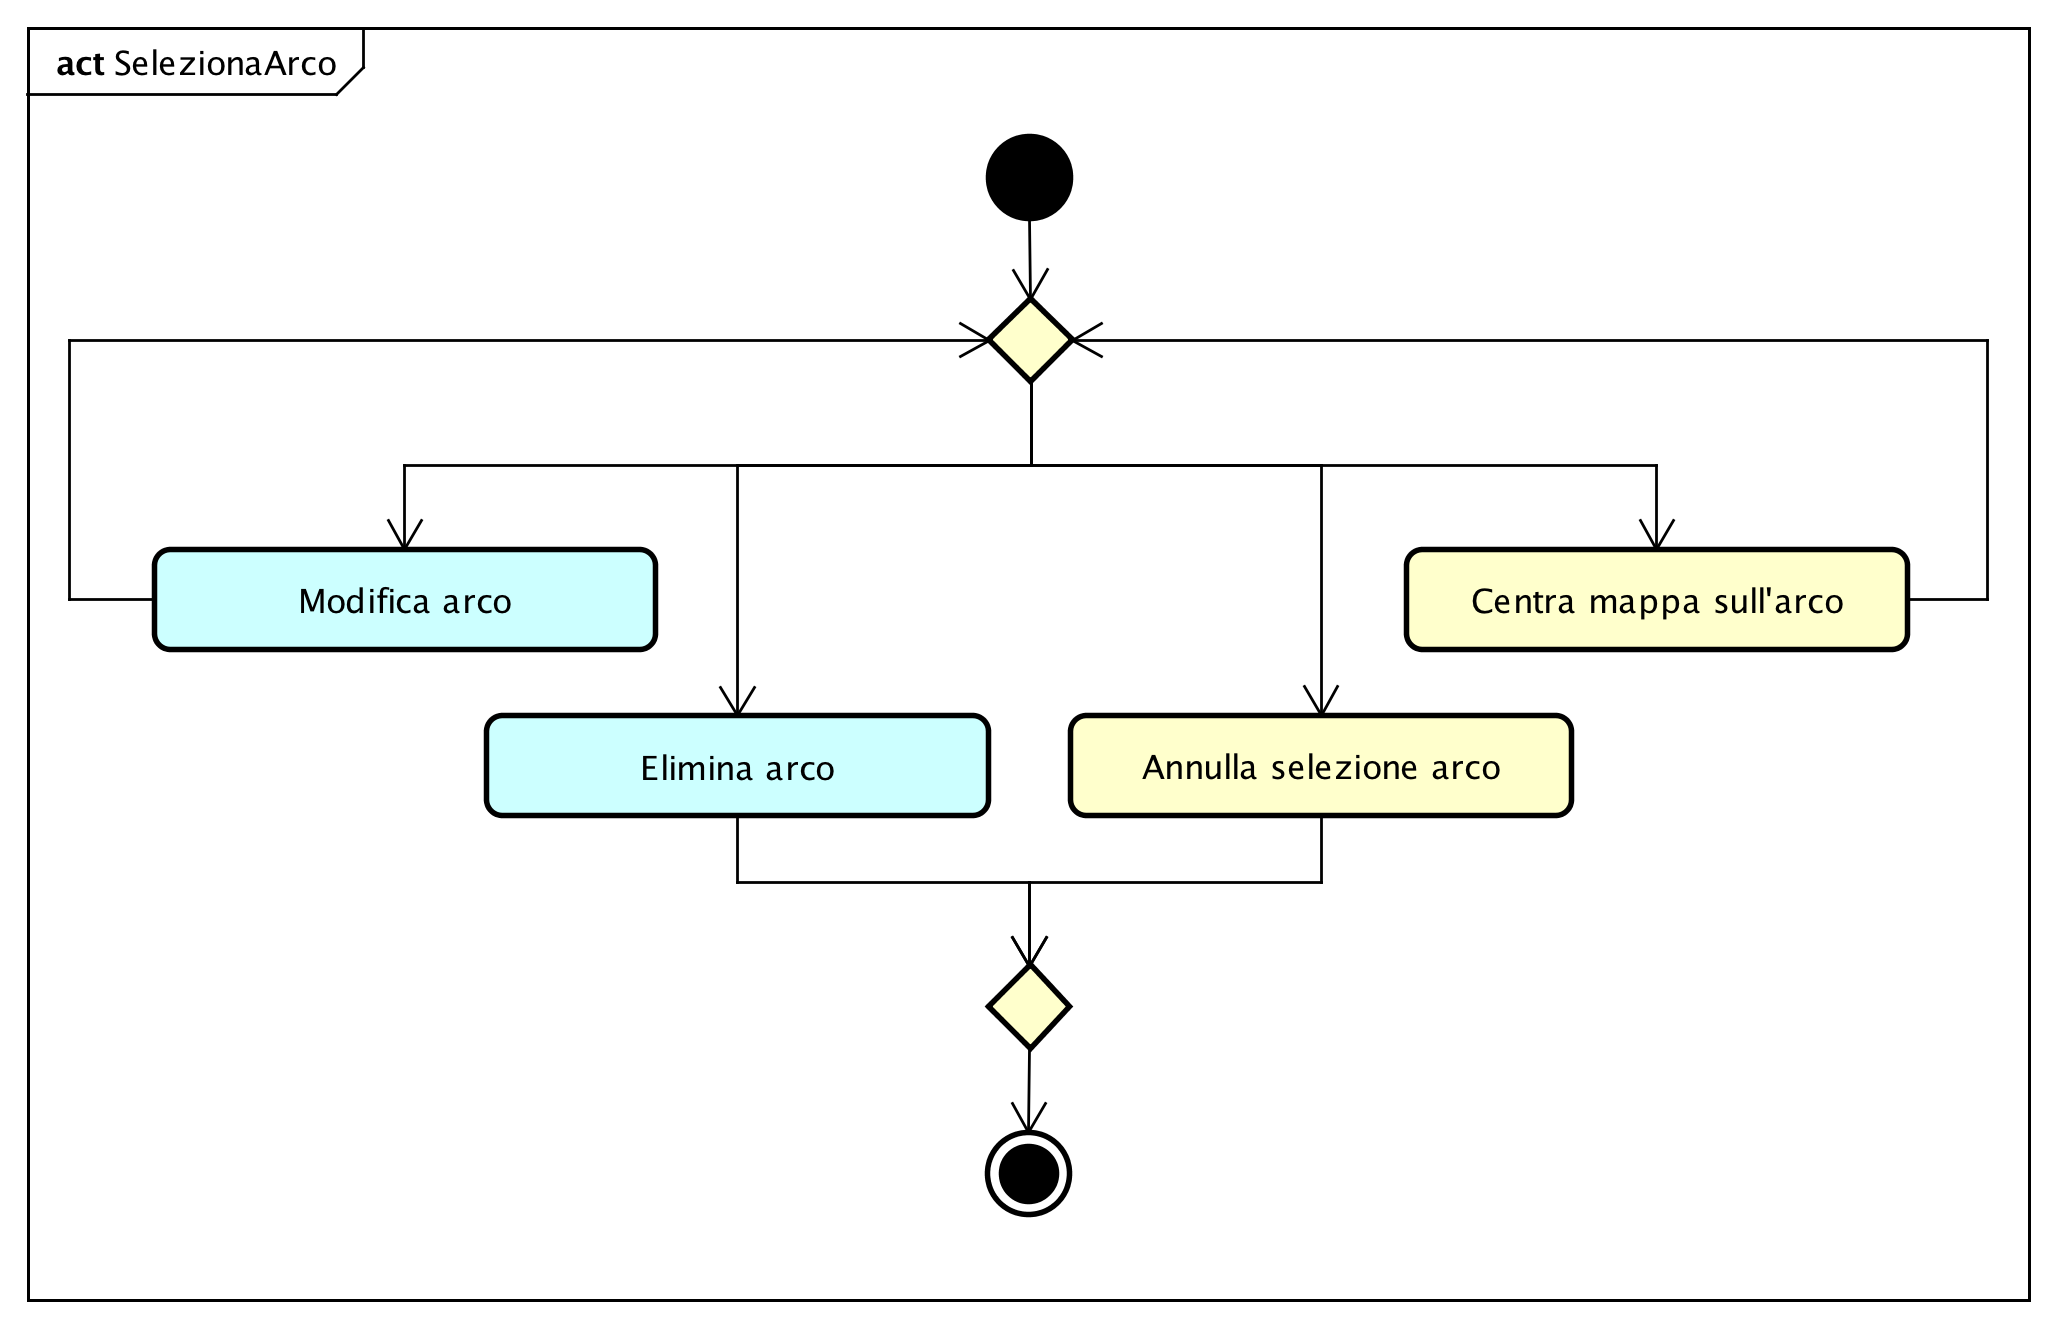
\includegraphics[width=\textwidth]{img/DiagrammiDiAttivita/SelezioneArco.png}
	\caption{Diagramma di attività per la selezione di un arco}
\end{figure}

\newpage
\subsection{Selezione scenario}
Una volta selezionato lo scenario l'utente potrà:
\begin{itemize}
	\item annullarne la selezione;
	\item selezionare un altro scenario;
	\item modificarlo;
	\item eliminarlo.
\end{itemize}
\begin{figure}[H]
	\centering
	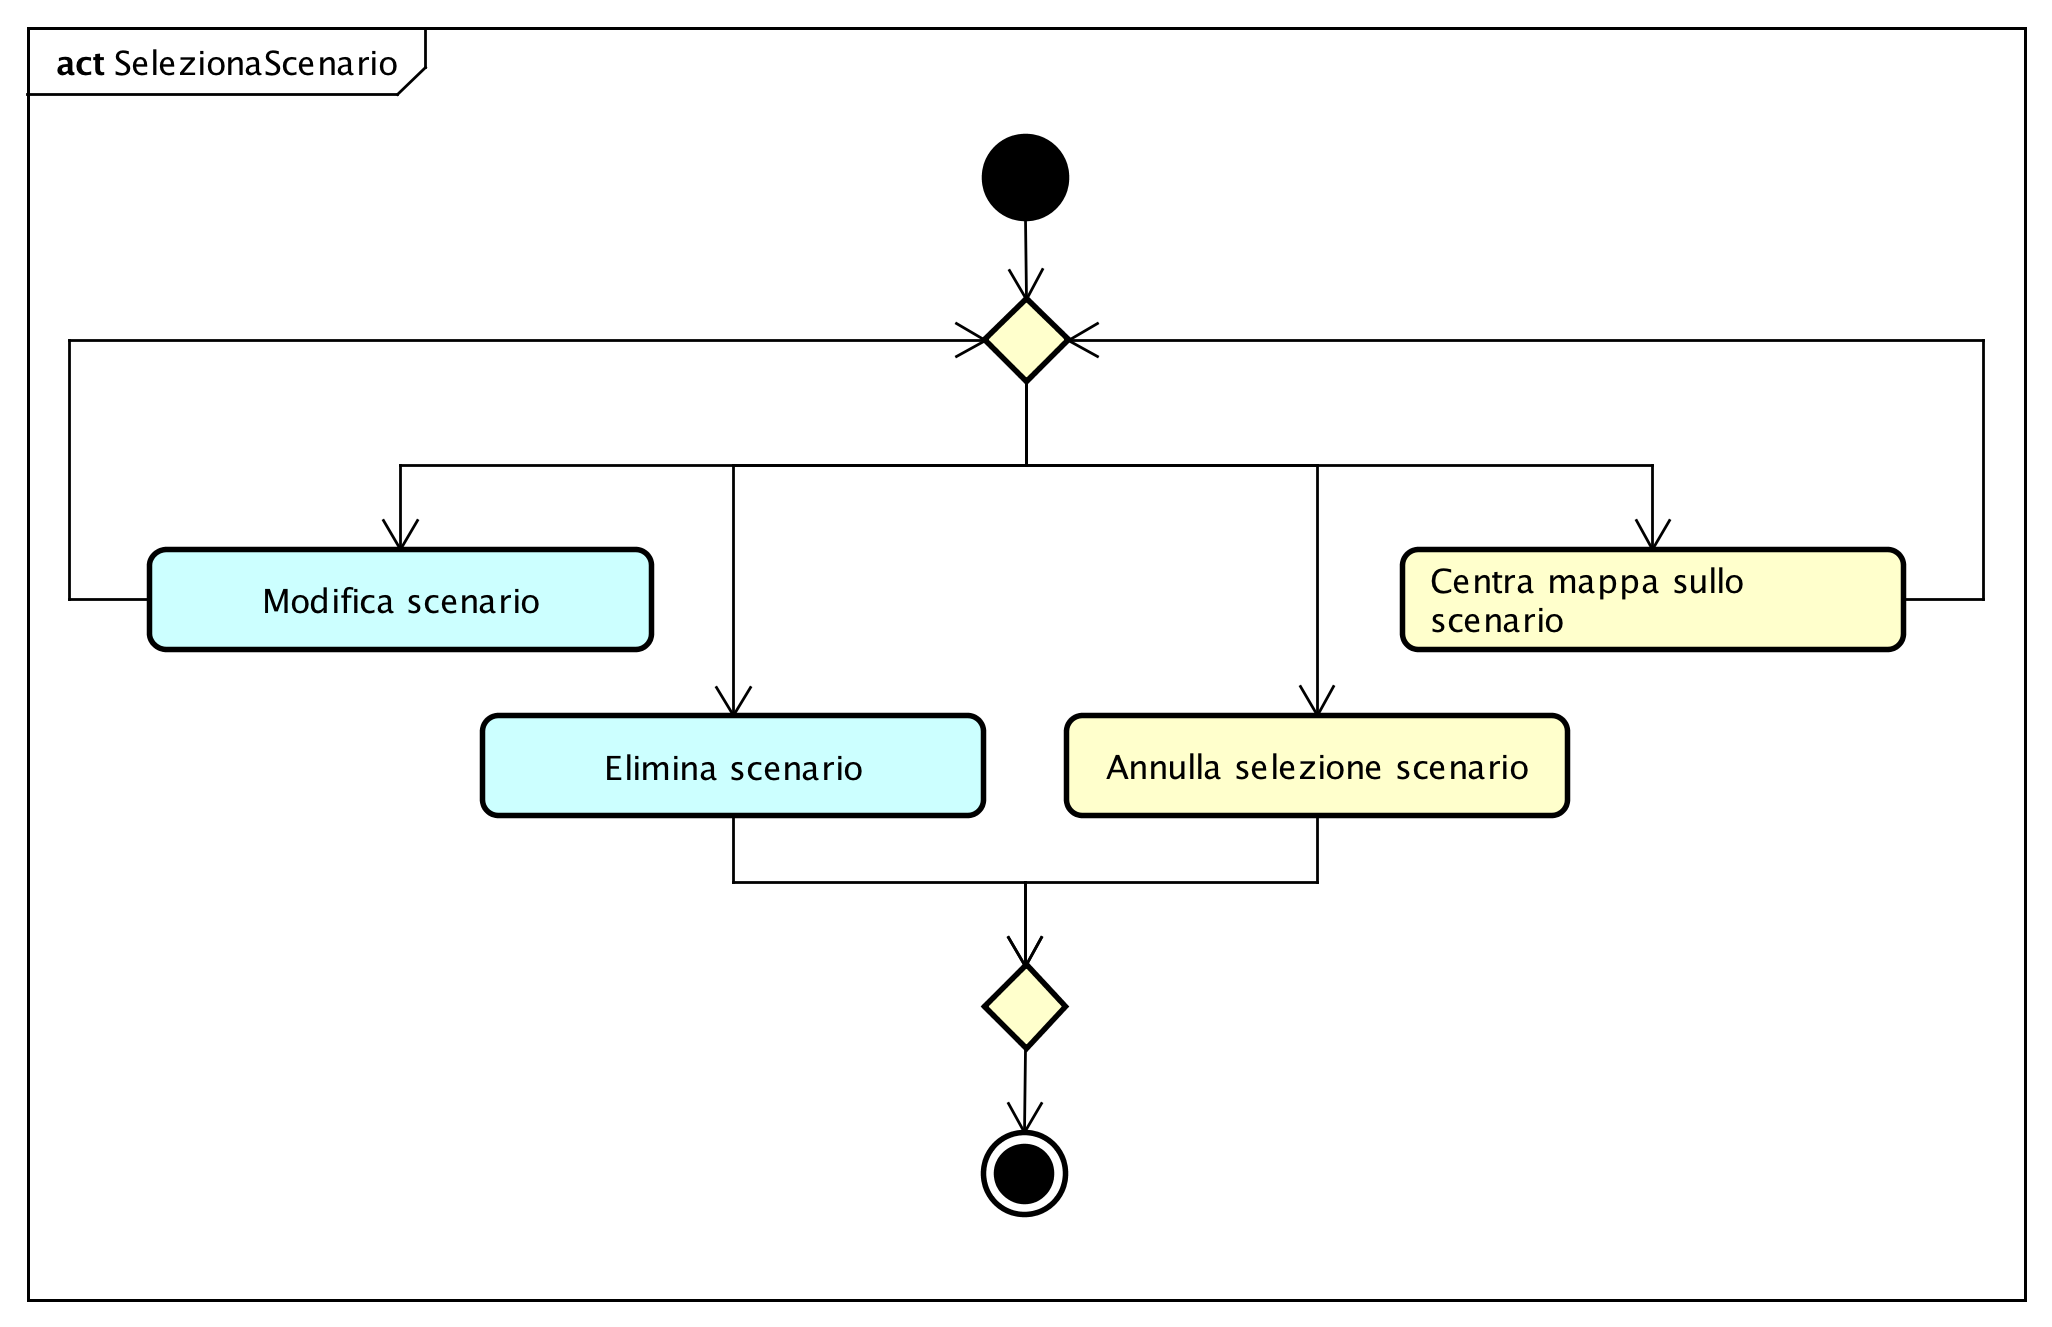
\includegraphics[width=\textwidth]{img/DiagrammiDiAttivita/SelezioneScenario.png}
	\caption{Diagramma di attività per la selezione di uno scenario}
\end{figure}
\begin{figure}[H]
	\centering
	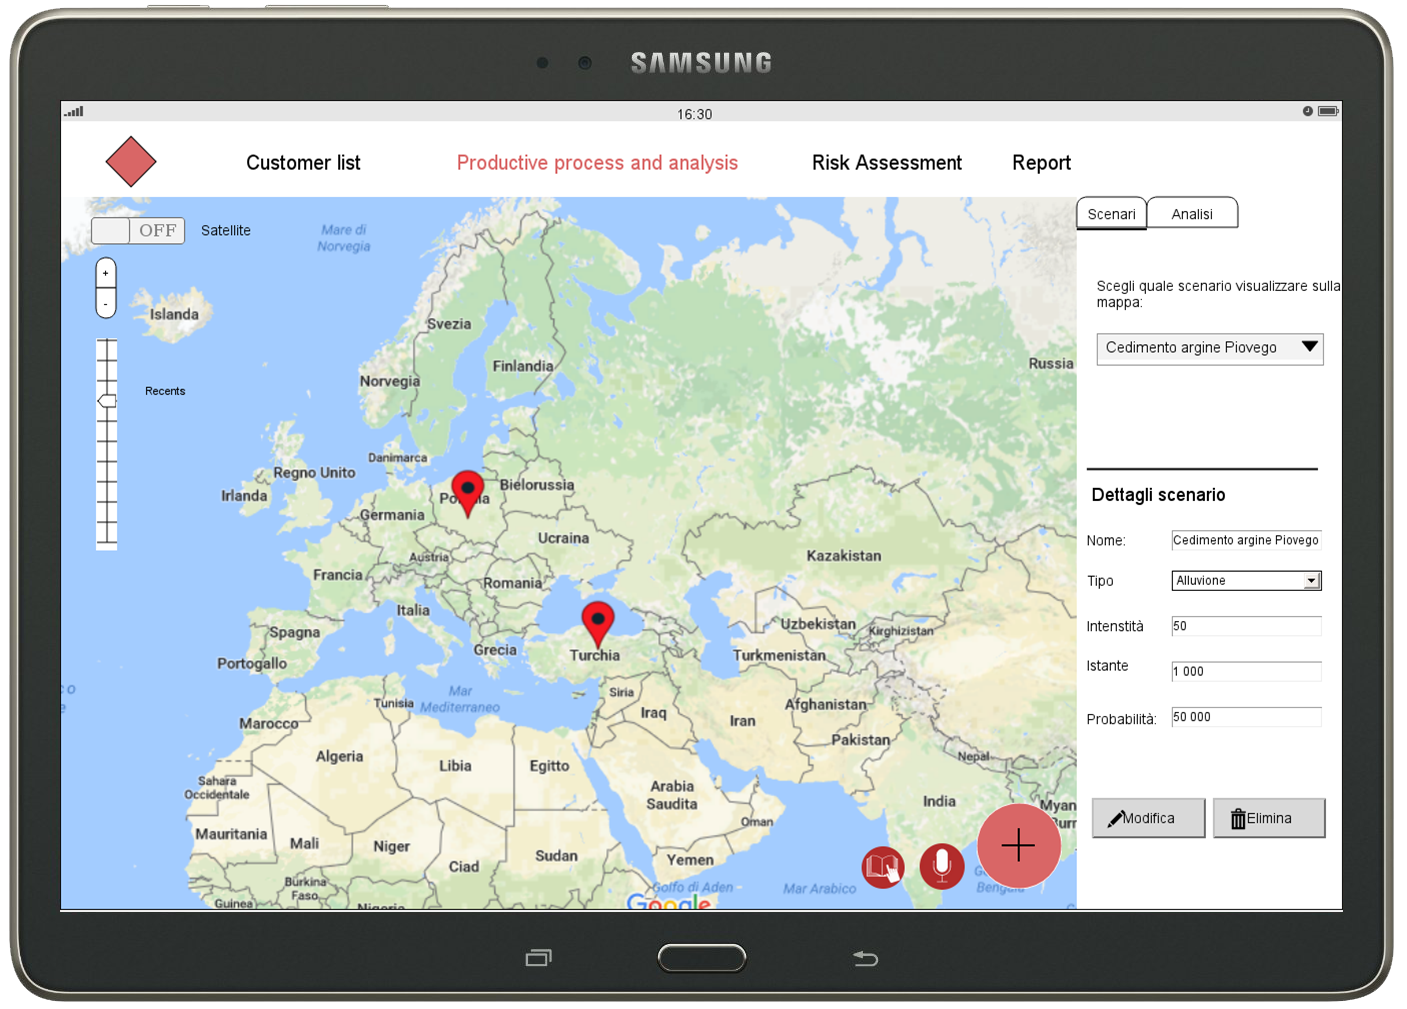
\includegraphics[width=\textwidth]{img/MockUp/m1.png}
	\caption{Mockup per la selezione di uno scenario}
\end{figure}

\newpage
\subsection{Modifica asset}
Per quanto riguarda la modifica dell'asset, sarà possibile ridisegnarne il perimetro dell'asset sulla mappa e/o modificarne i dati precedentemente compilati. Infine si dovrà confermare la modifica. In caso di dati non corretti, la modifica potrebbe non andare a buon fine: verrà visualizzato un messaggio di errore e l'utente sarà tenuto a correggere eventuali errori o incompletezze.
In ogni momento l'utente può annullare la modifica. Il sistema richiede una conferma per portare a termine tale operazione.
\begin{figure}[H]
	\centering
	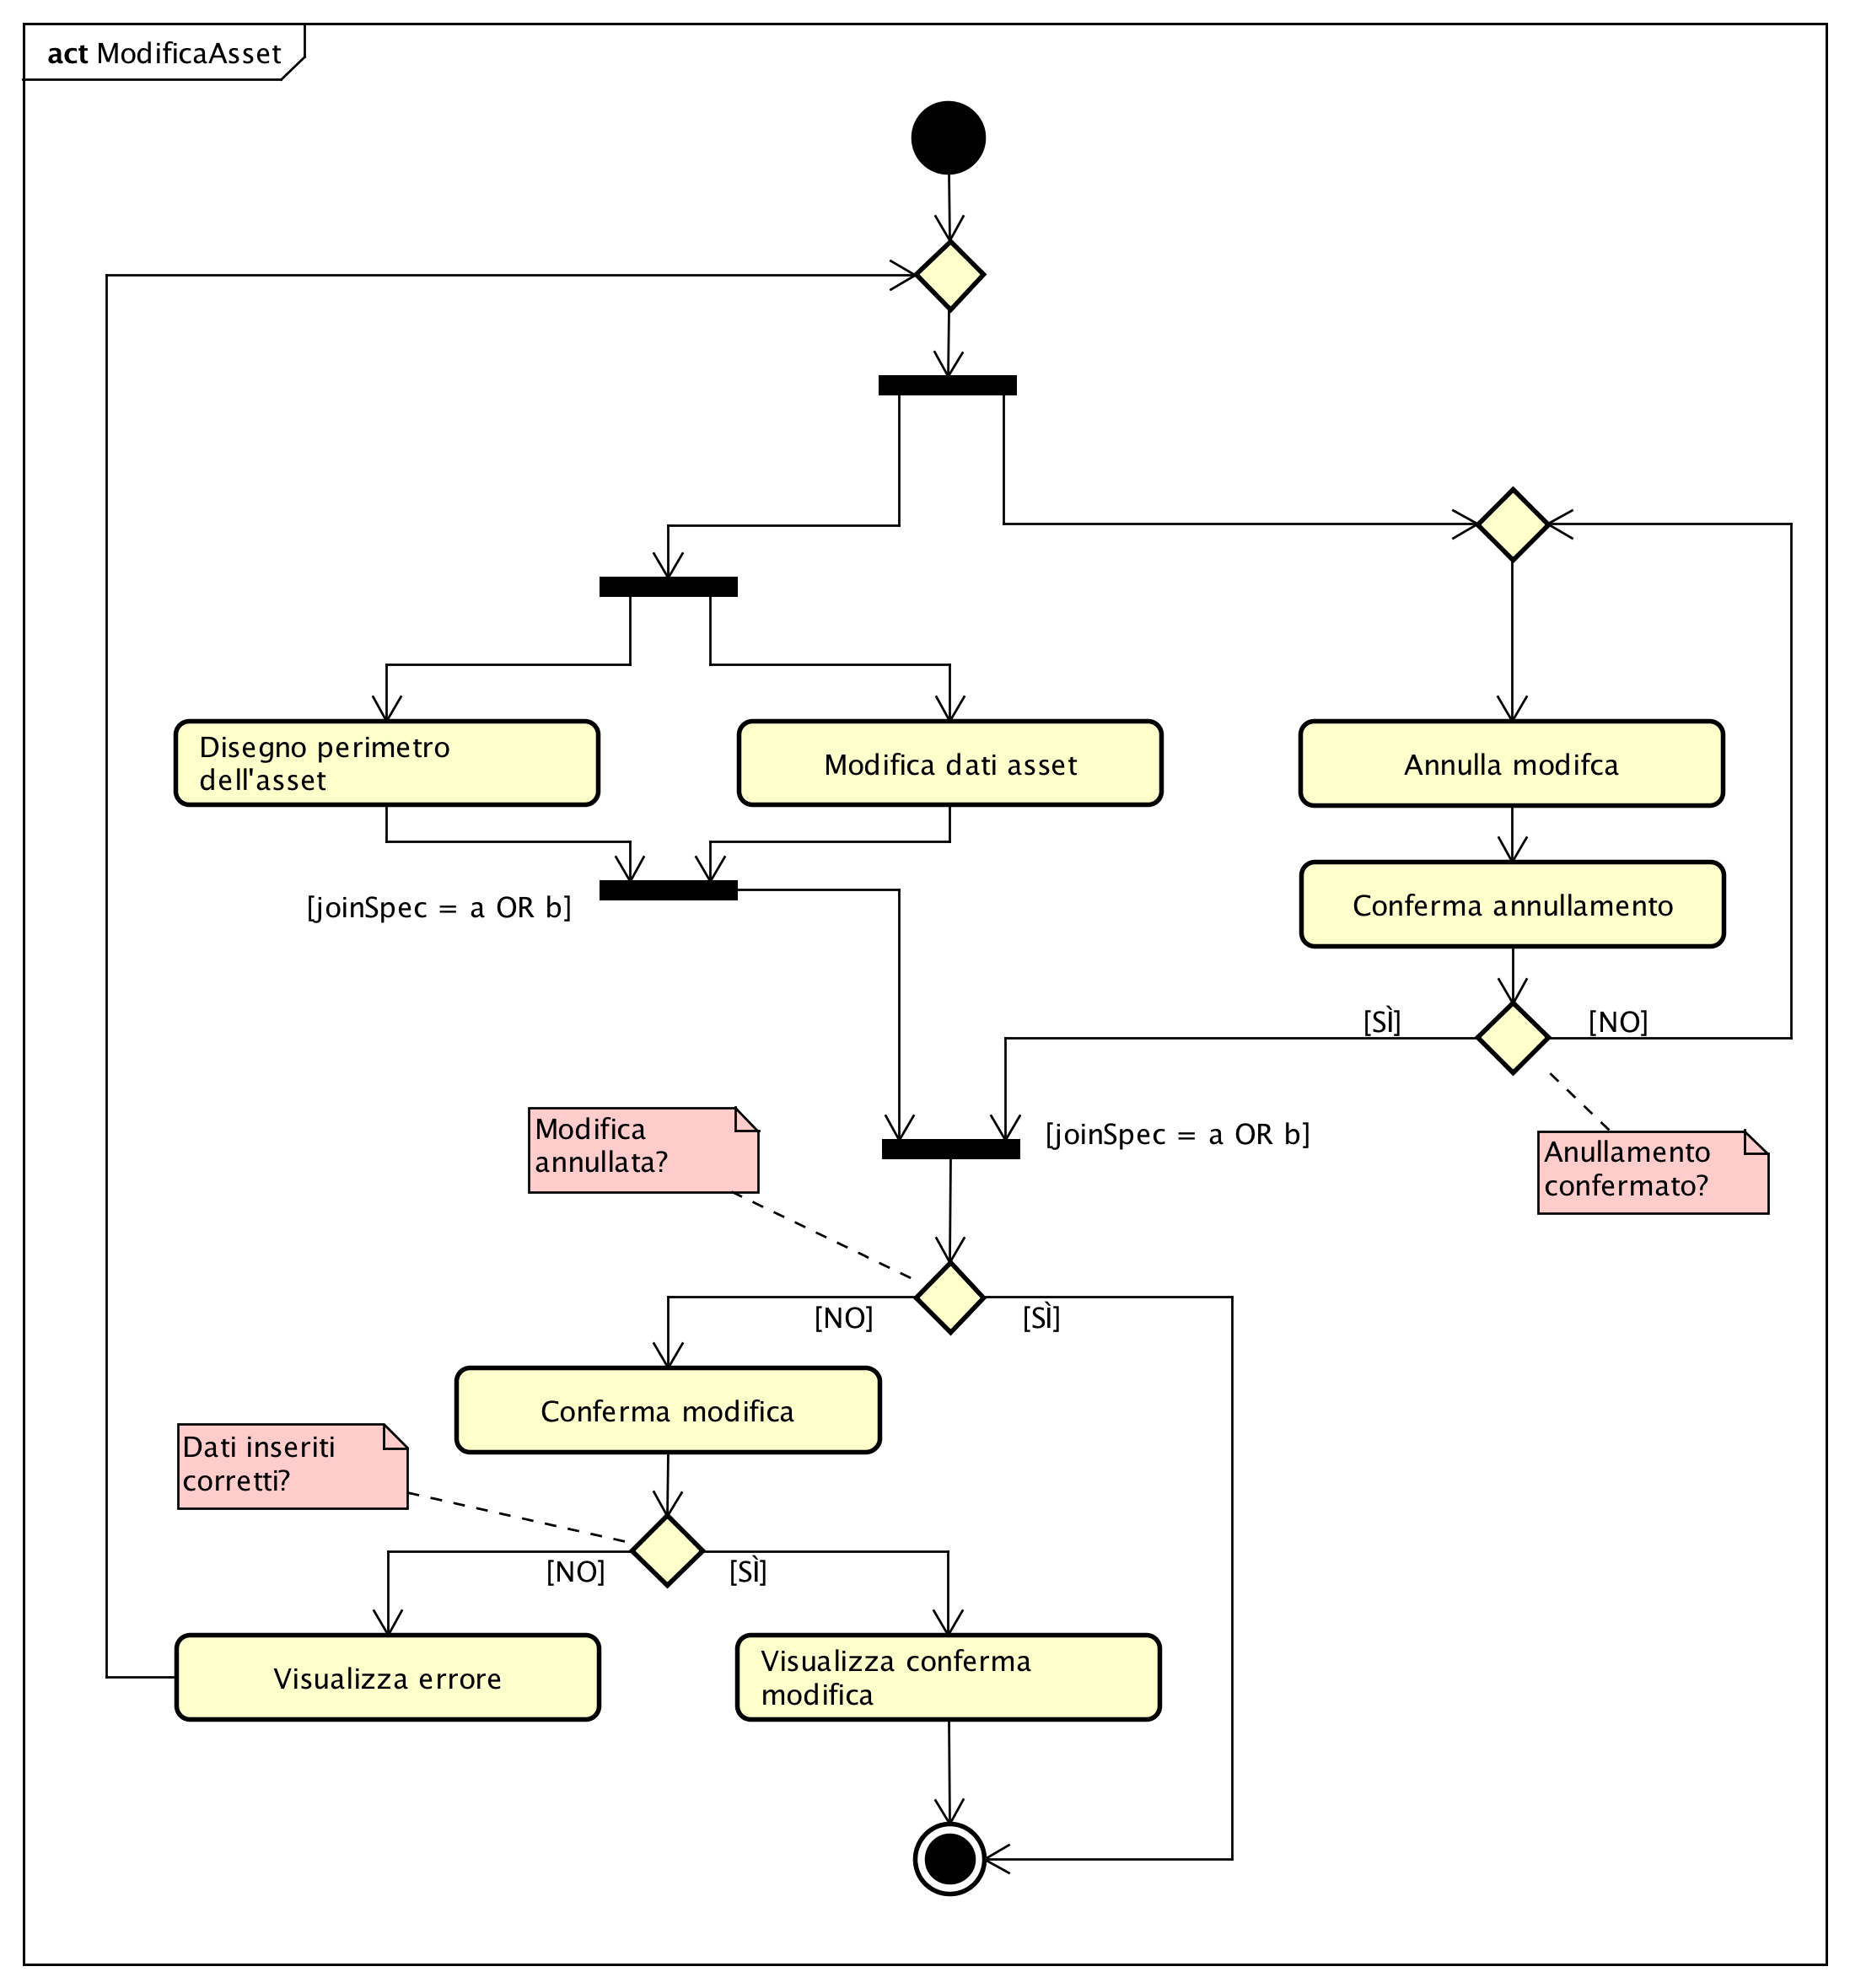
\includegraphics[width=\textwidth]{img/DiagrammiDiAttivita/ModificaAsset.png}
	\caption{Diagramma di attività per la modifica di un asset}
\end{figure}
\begin{figure}[H]
	\centering
	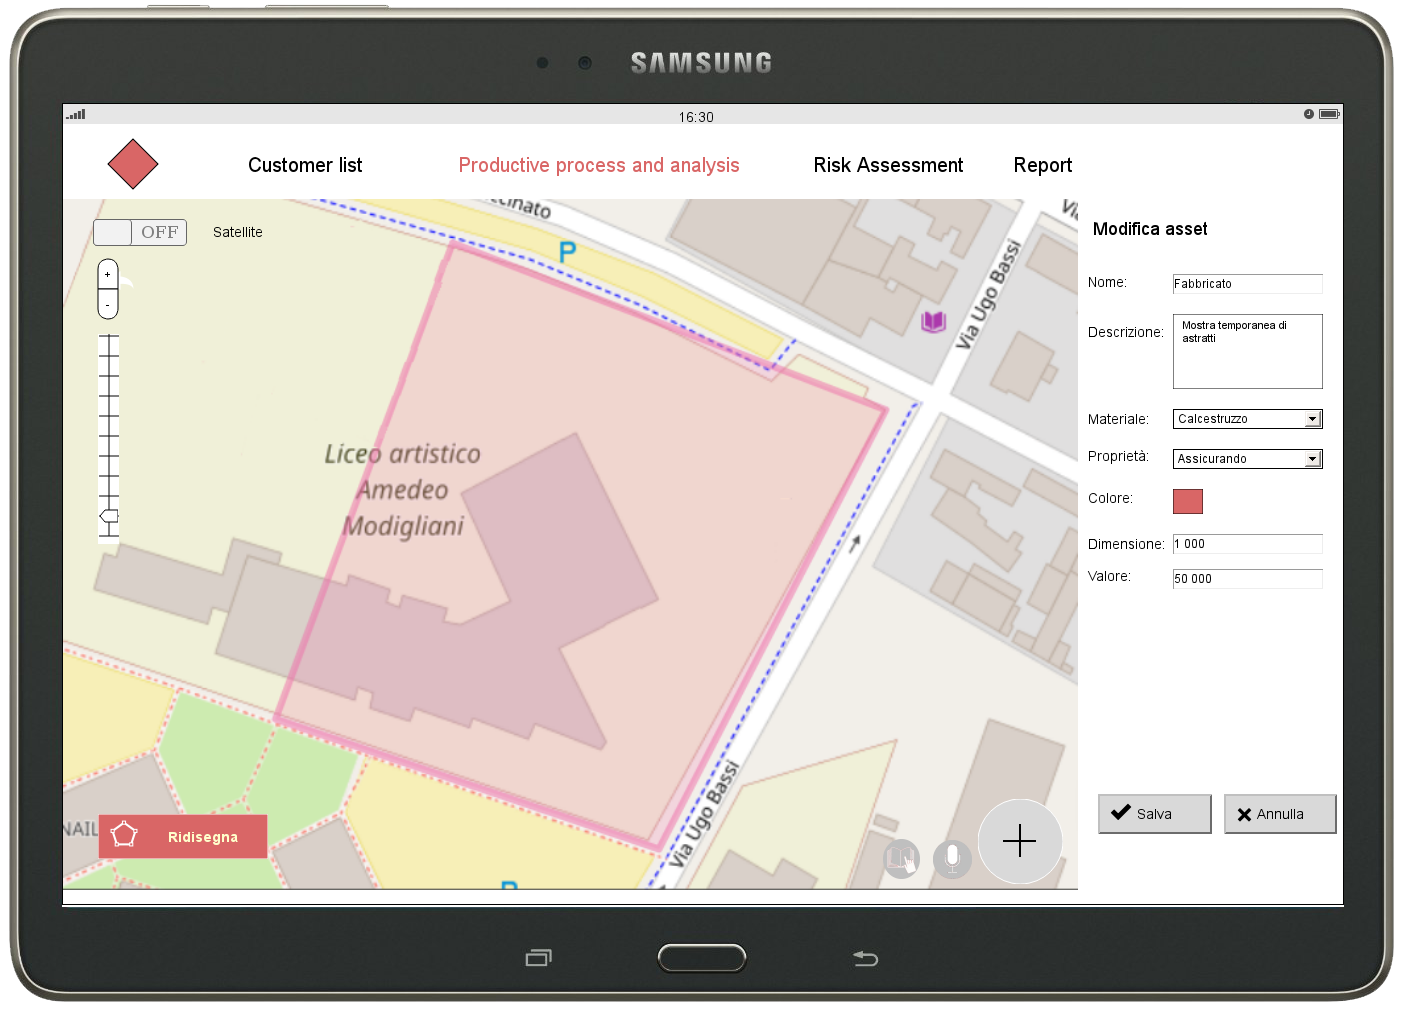
\includegraphics[width=\textwidth]{img/MockUp/m8.png}
	\caption{Mockup per la modifica di un asset}
\end{figure}

\newpage
\subsection{Modifica nodo}
Per quanto riguarda la modifica del nodo, sarà possibile riposizionare il nodo sulla mappa e/o modificarne i dati precedentemente compilati. Infine si dovrà confermare la modifica. In caso di dati non corretti, la modifica potrebbe non andare a buon fine: verrà visualizzato un messaggio di errore e l'utente sarà tenuto a correggere eventuali errori o incompletezze.
In ogni momento l'utente può annullare la modifica. Il sistema richiede una conferma per portare a termine tale operazione.
\begin{figure}[H]
	\centering
	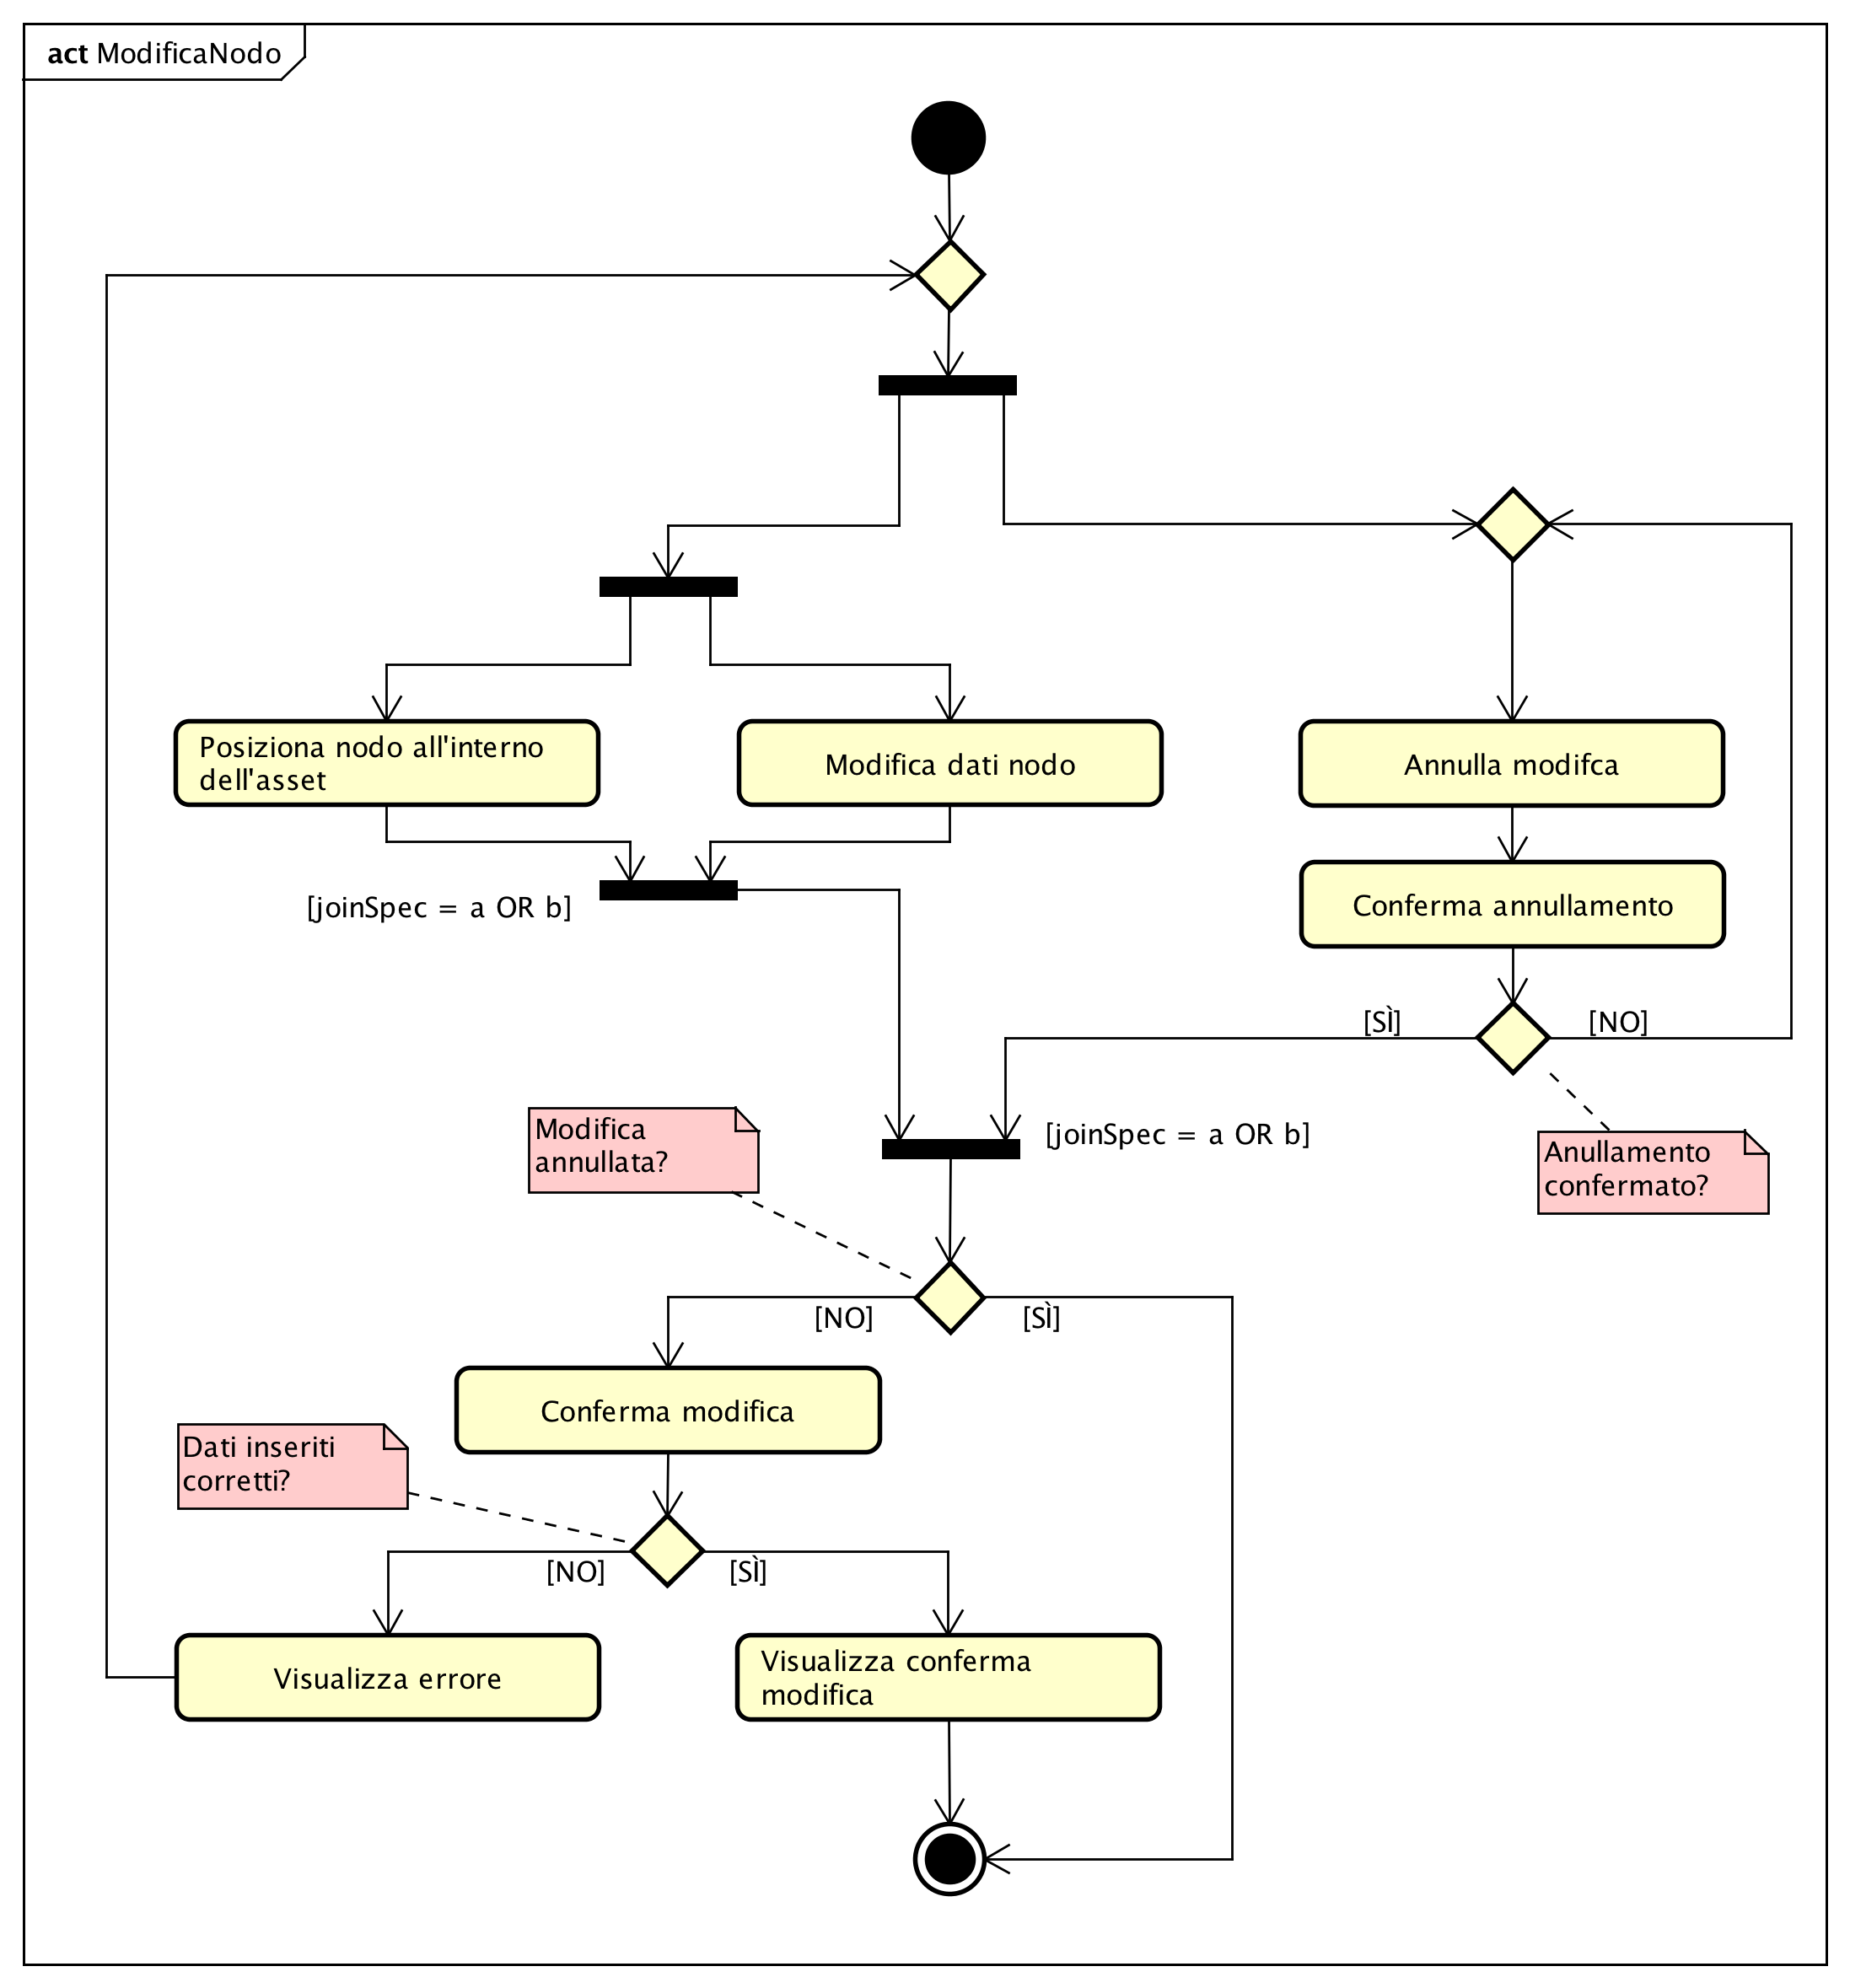
\includegraphics[width=\textwidth]{img/DiagrammiDiAttivita/ModificaNodo.png}
	\caption{Diagramma di attività per la modifica di un nodo}
\end{figure}
\begin{figure}[H]
	\centering
	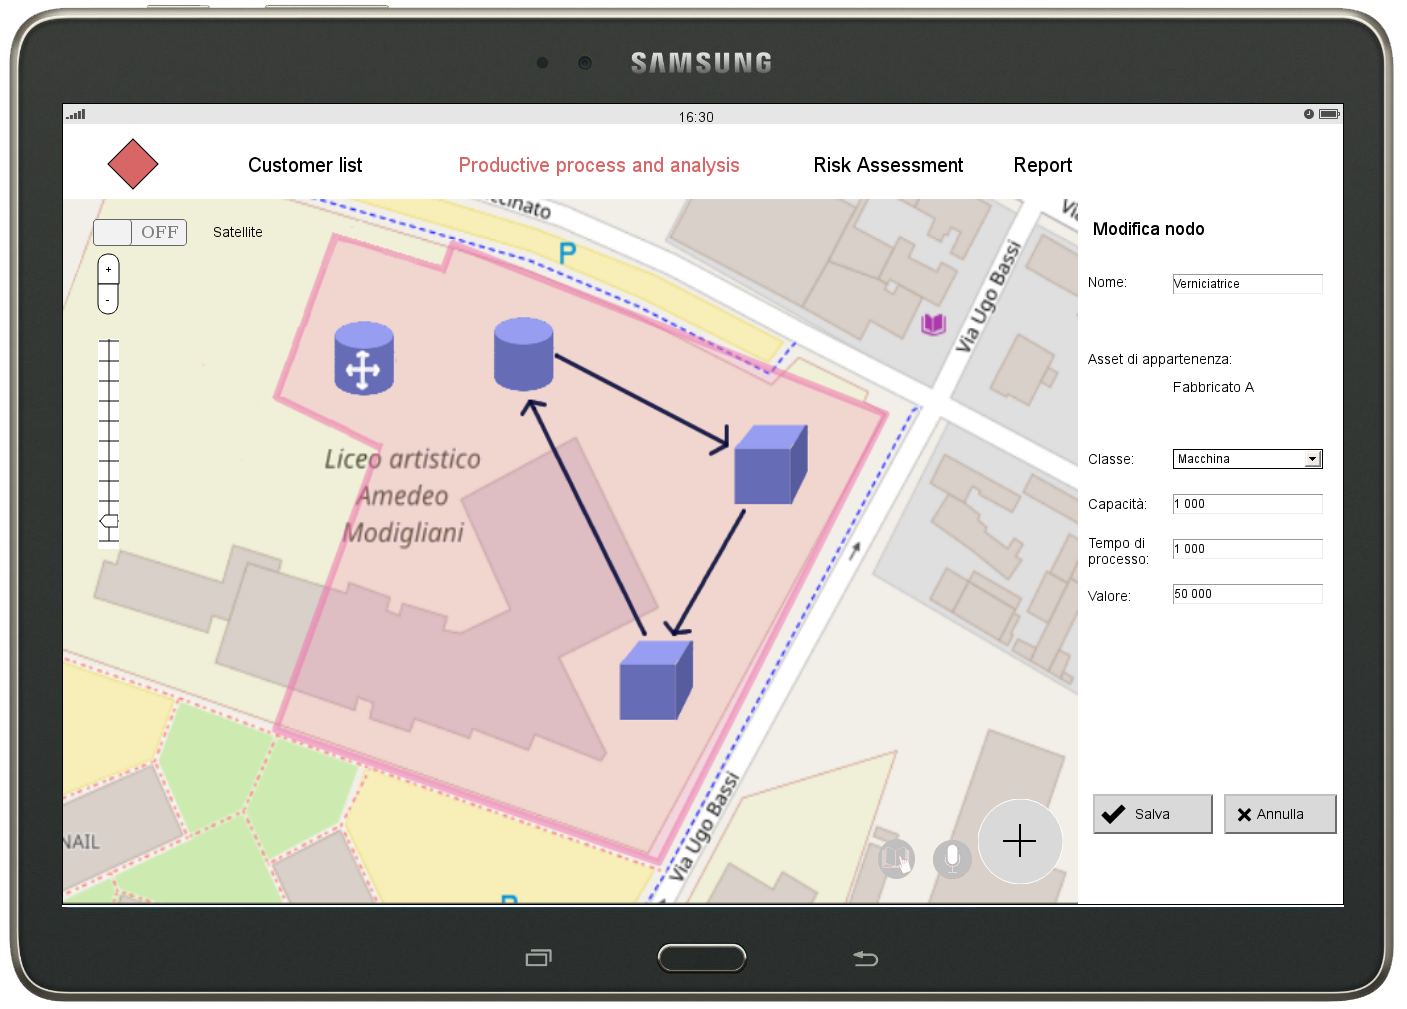
\includegraphics[width=\textwidth]{img/MockUp/m14.png}
	\caption{Mockup per la modifica di un nodo}
\end{figure}

\newpage
\subsection{Modifica arco}
Per quanto riguarda la modifica dell'arco, sarà possibile ridisegnare l'arco sulla mappa e/o modificarne i dati precedentemente compilati. Infine si dovrà confermare la modifica. In caso di dati non corretti, la modifica potrebbe non andare a buon fine: verrà visualizzato un messaggio di errore e l'utente sarà tenuto a correggere eventuali errori o incompletezze.
In ogni momento l'utente può annullare la modifica. Il sistema richiede una conferma per portare a termine tale operazione.
\begin{figure}[H]
	\centering
	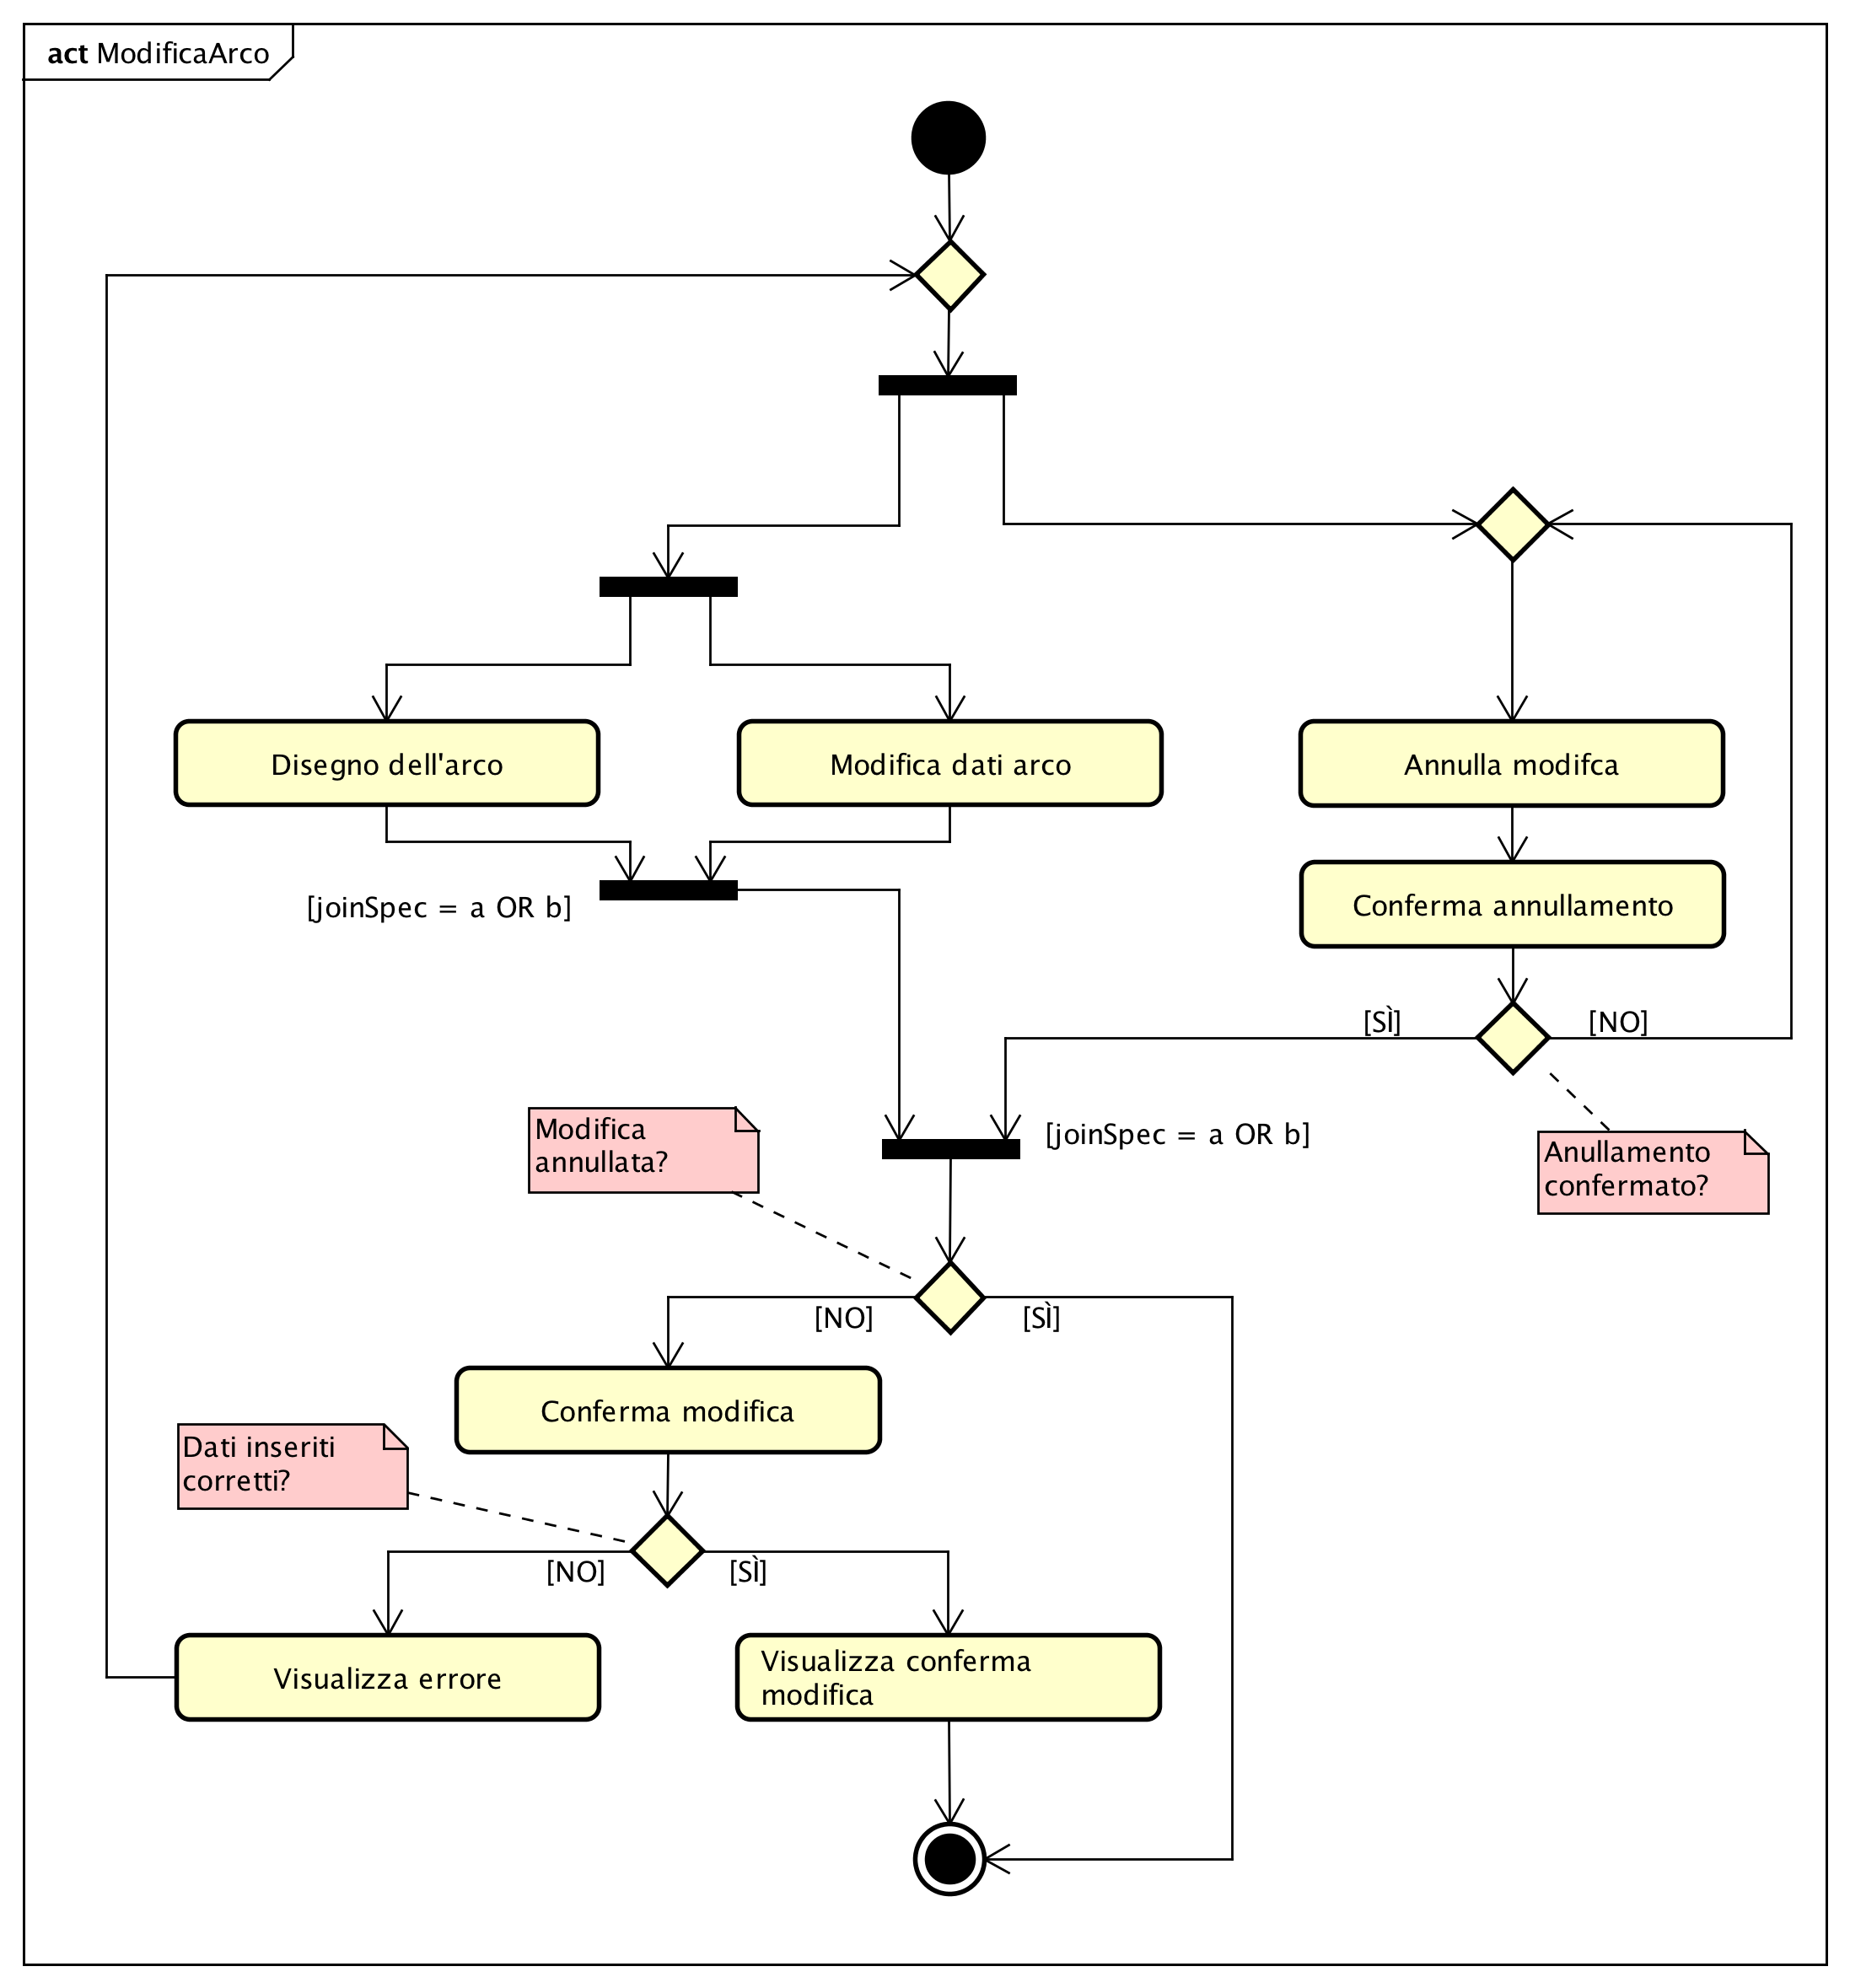
\includegraphics[width=\textwidth]{img/DiagrammiDiAttivita/ModificaArco.png}
	\caption{Diagramma di attività per la modifica di un arco}
\end{figure}

\newpage
\subsection{Modifica scenario}
Per quanto riguarda la modifica dello scenario, sarà possibile ridisegnarne il perimetro dell'asset sulla mappa e/o modificarne i dati precedentemente compilati. Infine si dovrà confermare la modifica. In caso di dati non corretti, la modifica potrebbe non andare a buon fine: verrà visualizzato un messaggio di errore e l'utente sarà tenuto a correggere eventuali errori o incompletezze.
In ogni momento l'utente può annullare la modifica. Il sistema richiede una conferma per portare a termine tale operazione.
\begin{figure}[H]
	\centering
	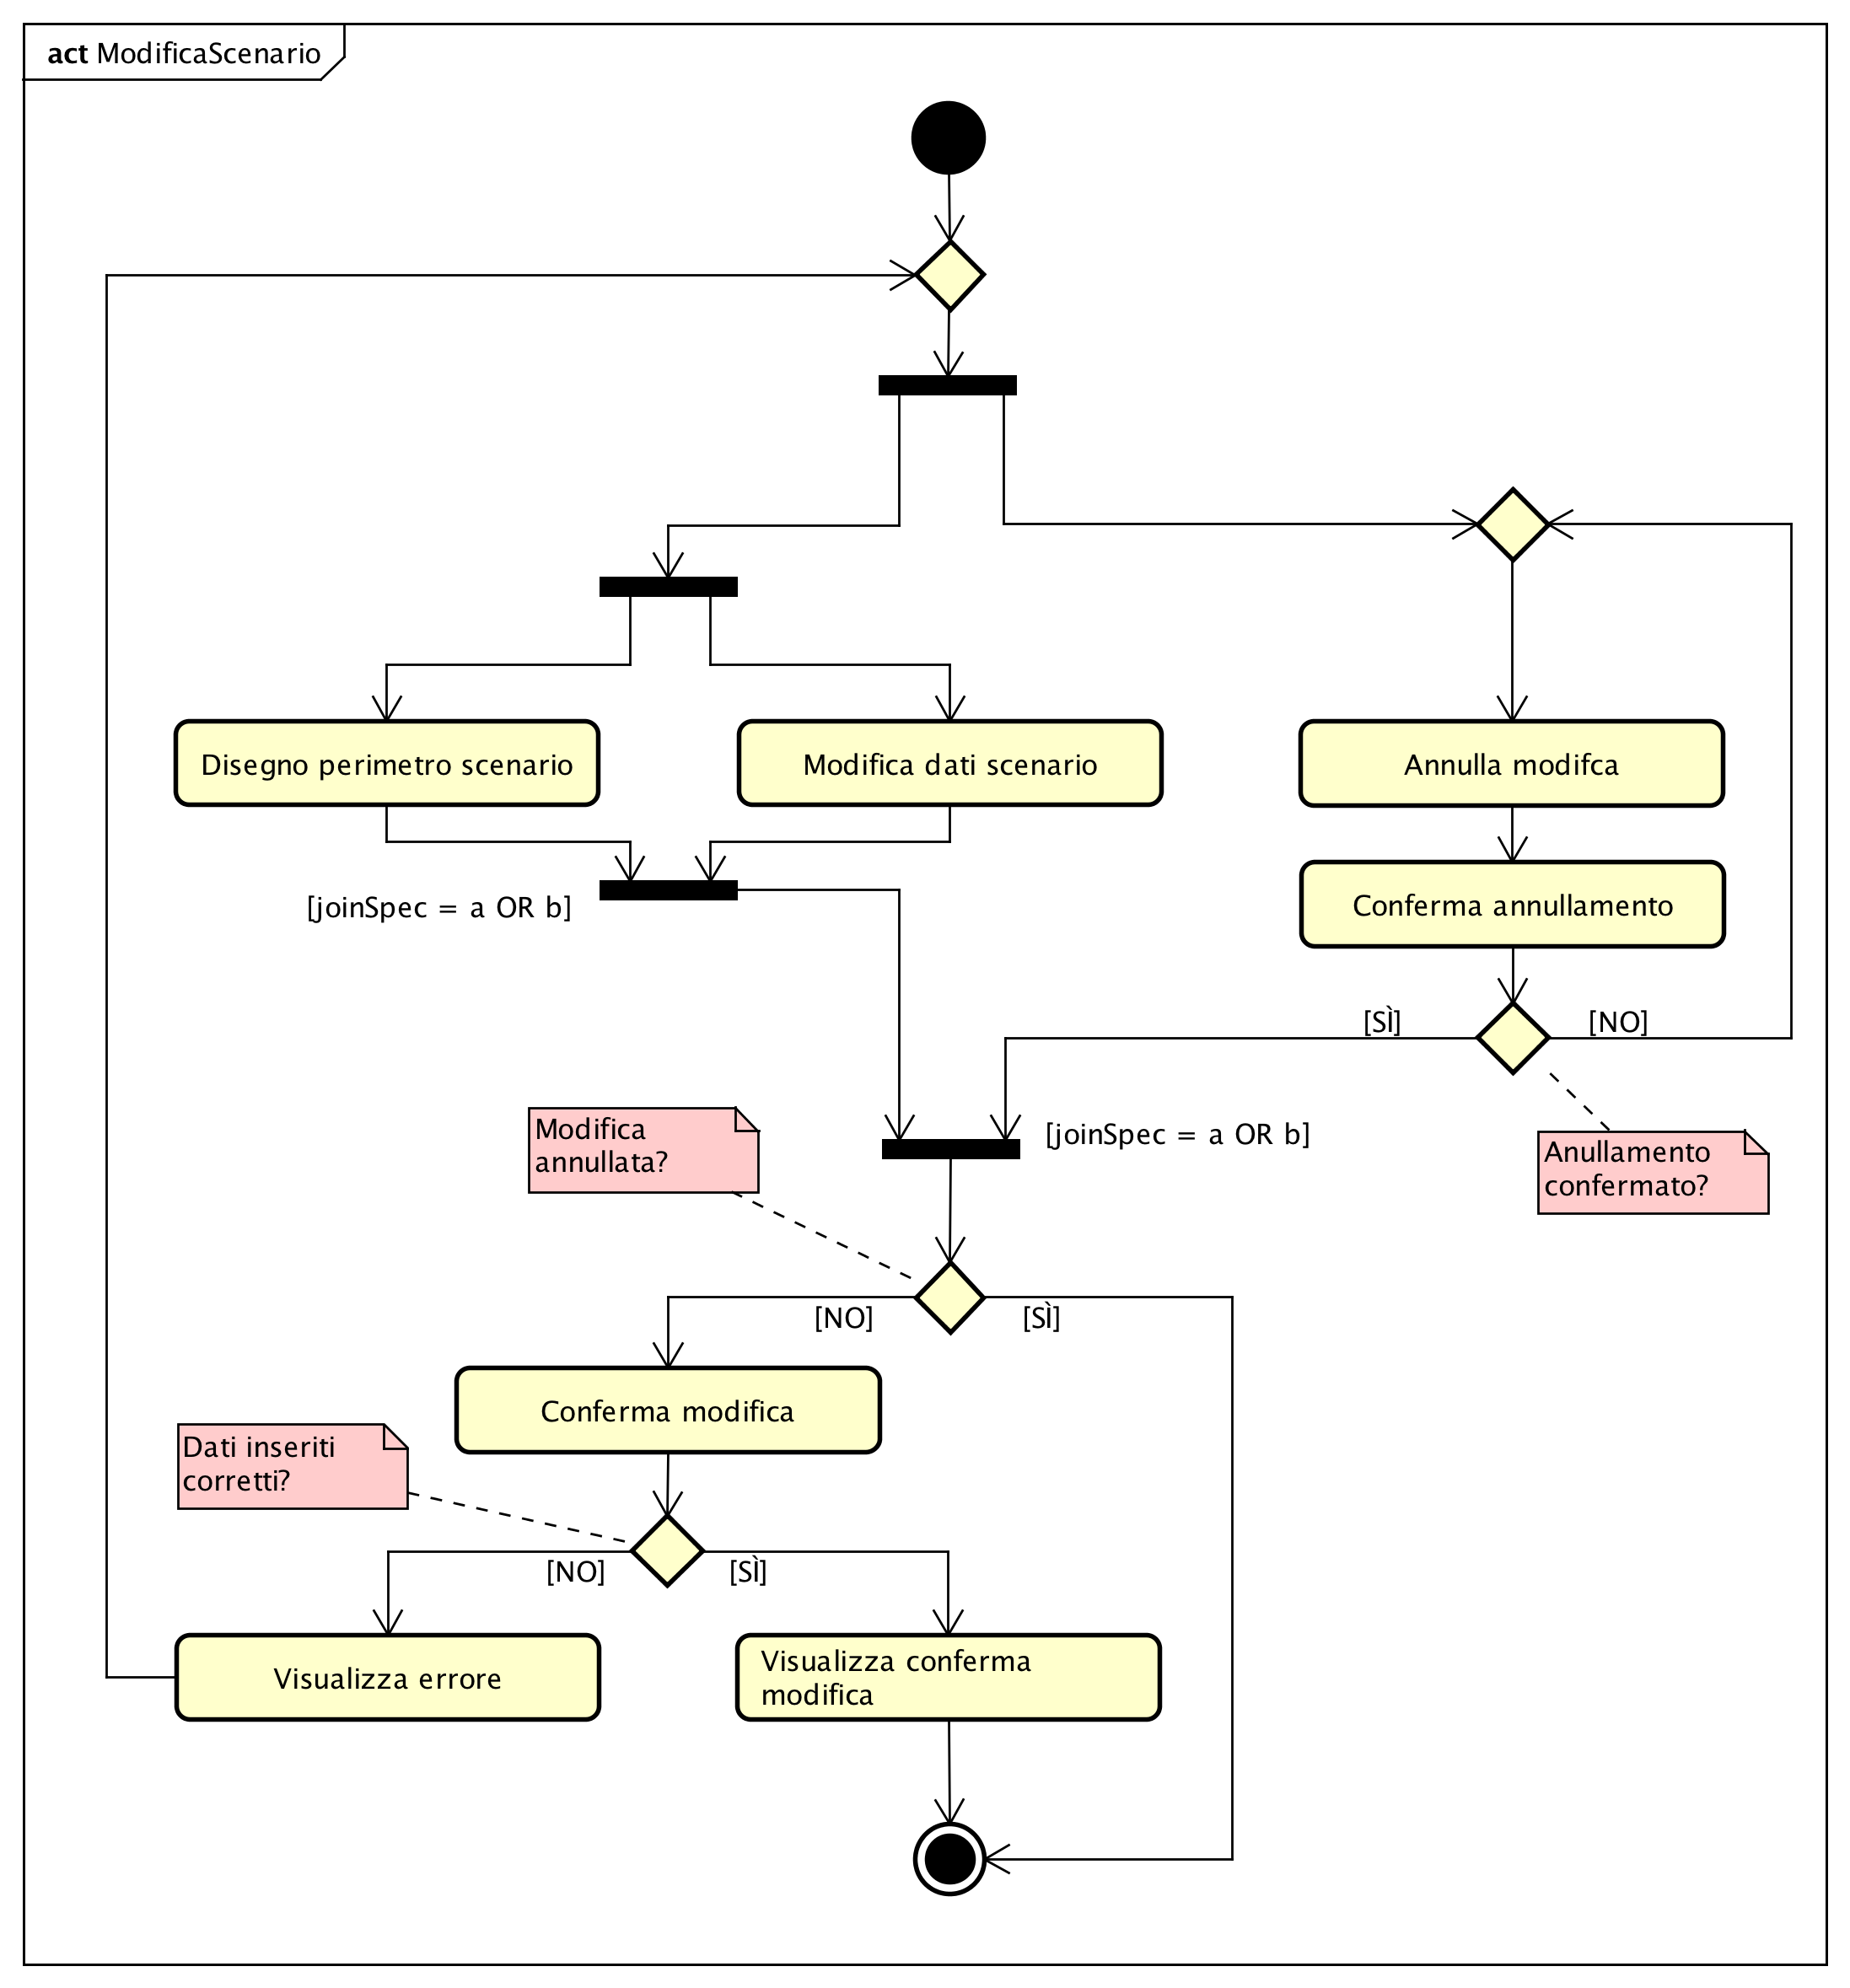
\includegraphics[width=\textwidth]{img/DiagrammiDiAttivita/ModificaScenario.png}
	\caption{Diagramma di attività per la modifica di uno scenario}
\end{figure}
\begin{figure}[H]
	\centering
	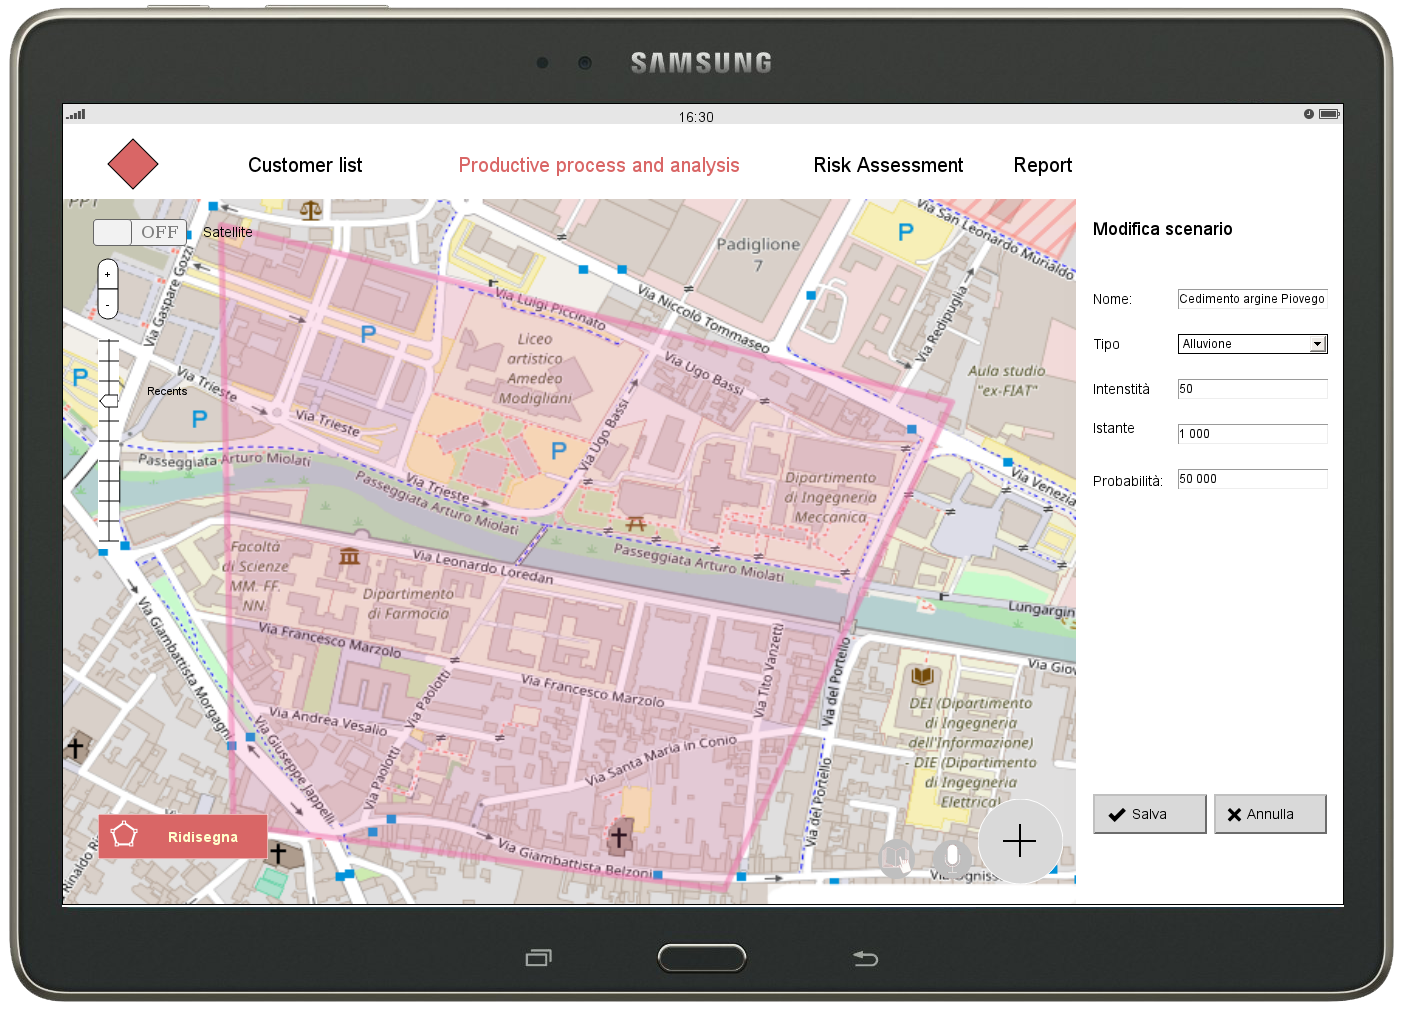
\includegraphics[width=\textwidth]{img/MockUp/m21.png}
	\caption{Mockup per la modifica di uno scenario}
\end{figure}

\newpage
\subsection{Eliminazione asset}
Una volta scelto di eliminare l'asset, l'utente è invitato a confermare l'eliminazione o ad annullarla.
\begin{figure}[H]
	\centering
	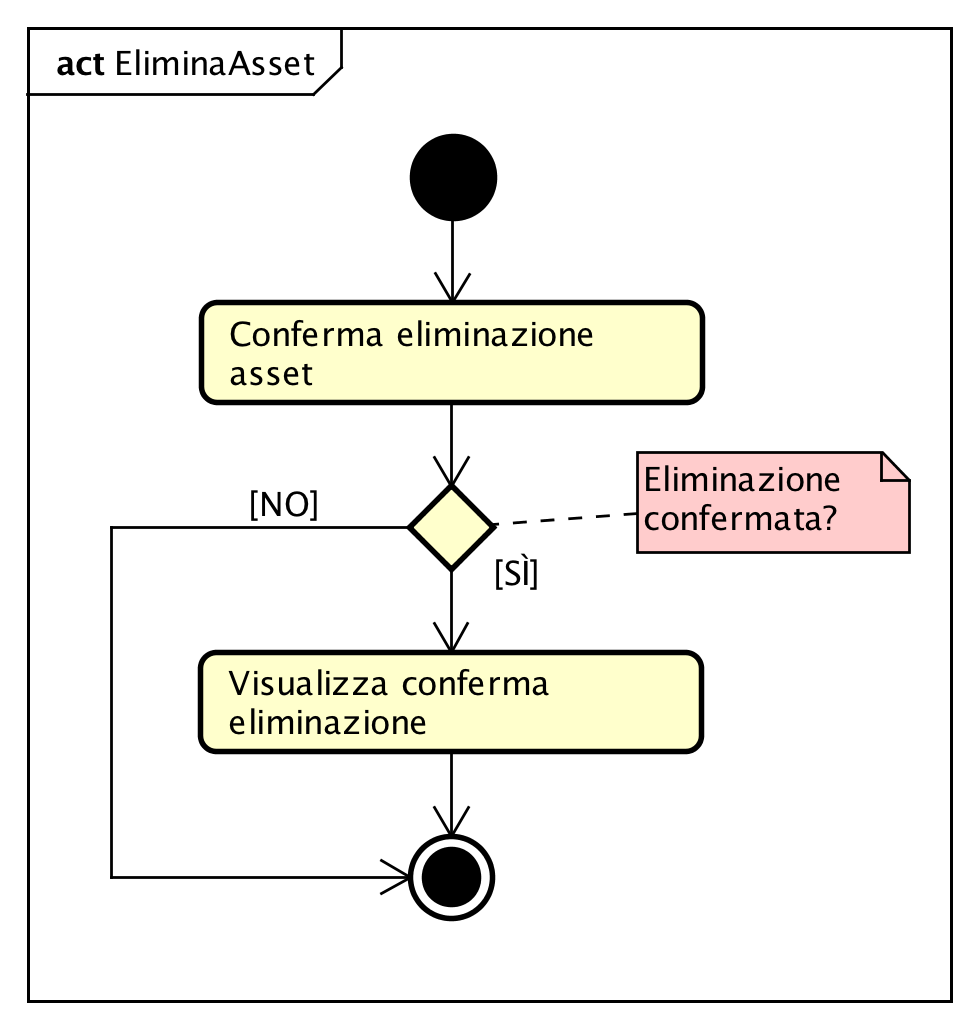
\includegraphics[scale=0.7]{img/DiagrammiDiAttivita/EliminazioneAsset.png}
	\caption{Diagramma di attività per l'eliminazione di un asset}
\end{figure}

\newpage
\subsection{Eliminazione nodo}
Una volta scelto di eliminare il nodo, l'utente è invitato a confermare l'eliminazione o ad annullarla.
\begin{figure}[H]
	\centering
	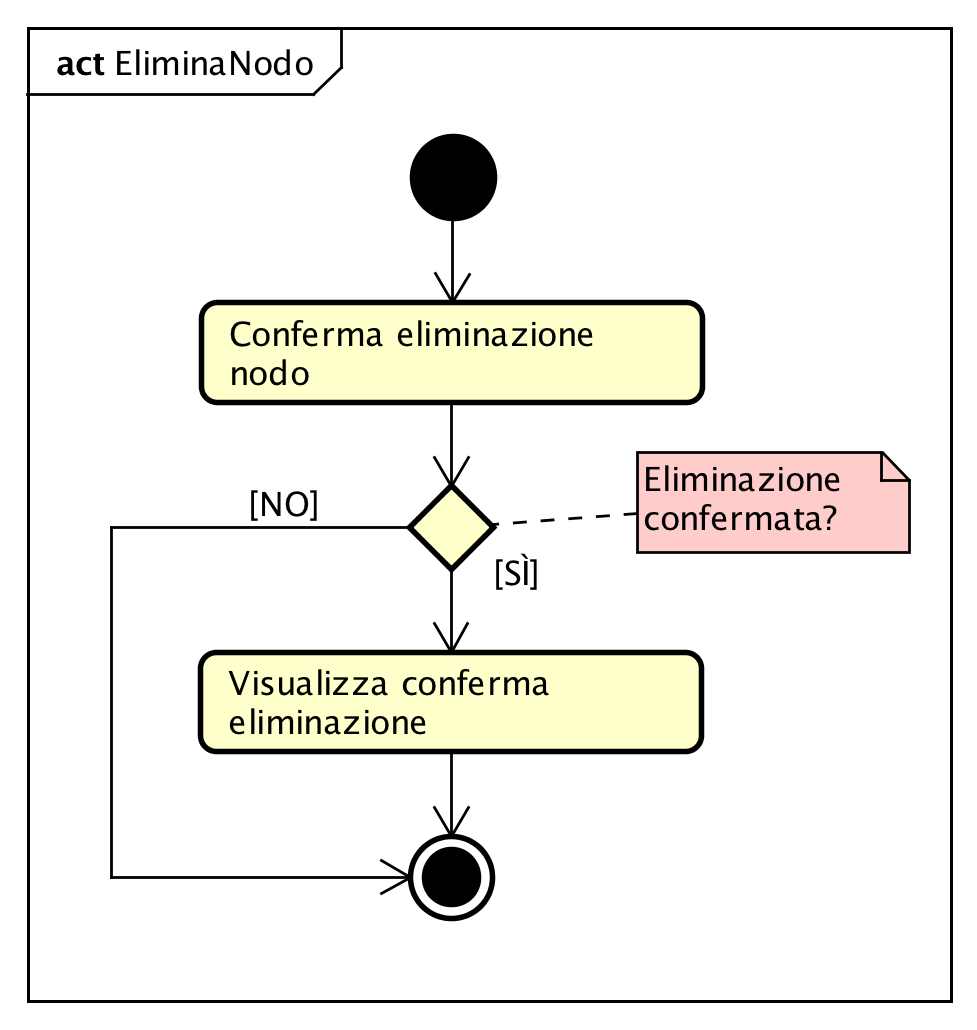
\includegraphics[scale=0.7]{img/DiagrammiDiAttivita/EliminazioneNodo.png}
	\caption{Diagramma di attività per l'eliminazione di un nodo}
\end{figure}
\begin{figure}[H]
	\centering
	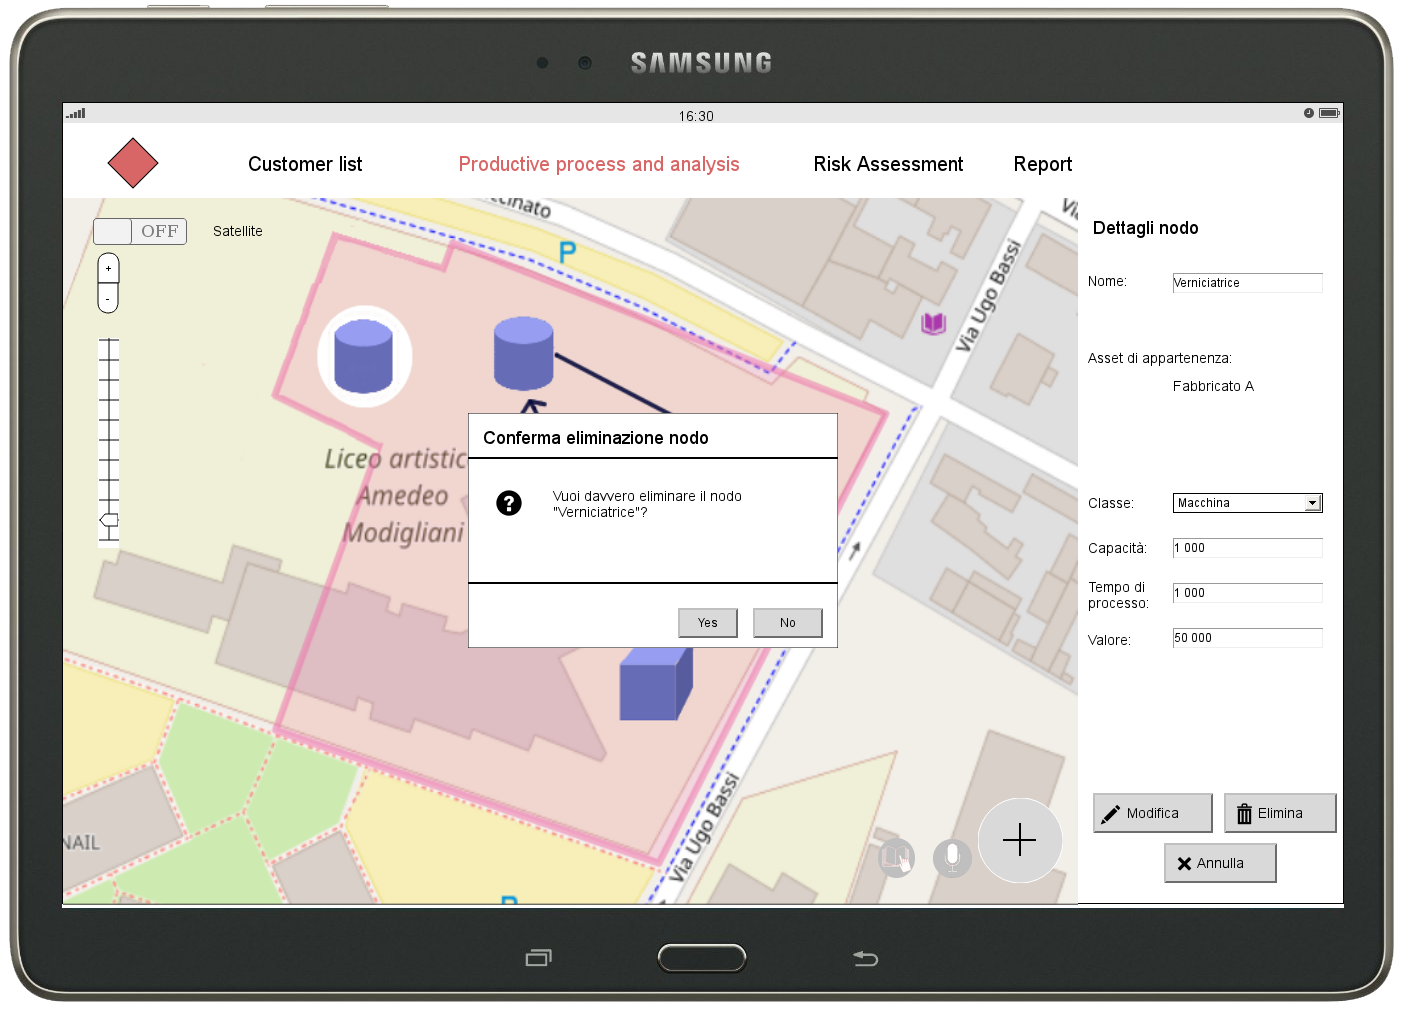
\includegraphics[width=\textwidth]{img/MockUp/m16.png}
	\caption{Mockup per l'eliminazione di un nodo}
\end{figure}


\newpage
\subsection{Eliminazione arco}
Una volta scelto di eliminare l'arco, l'utente è invitato a confermare l'eliminazione o ad annullarla.
\begin{figure}[H]
	\centering
	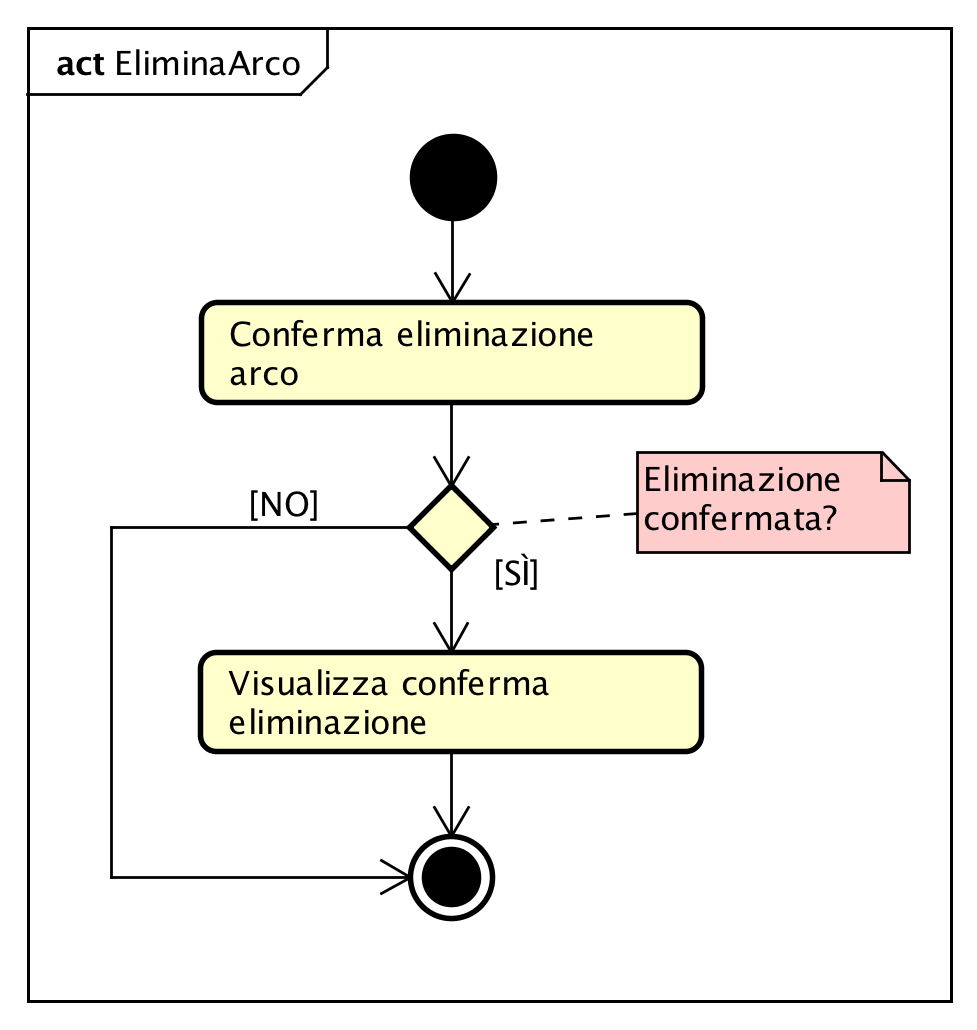
\includegraphics[scale=0.7]{img/DiagrammiDiAttivita/EliminazioneArco.png}
	\caption{Diagramma di attività per l'eliminazione di un arco}
\end{figure}

\newpage
\subsection{Eliminazione scenario}
Una volta scelto di eliminare lo scenario, l'utente è invitato a confermare l'eliminazione o ad annullarla.
\begin{figure}[H]
	\centering
	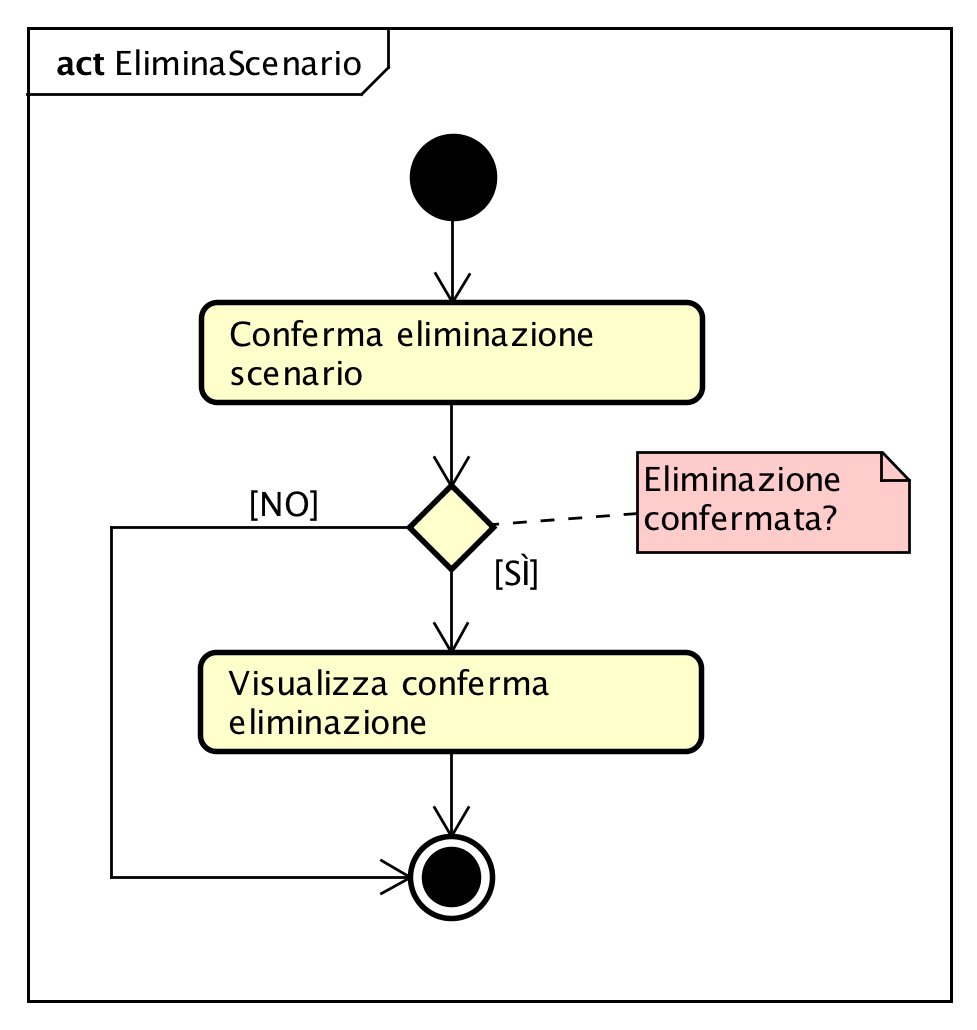
\includegraphics[scale=0.7]{img/DiagrammiDiAttivita/EliminazioneScenario.png}
	\caption{Diagramma di attività per l'eliminazione di uno scenario}
\end{figure}

\newpage
\subsection{Errore di connessione}
In caso di errori di connessione compare un messaggio di errore. In questo caso l'utente può chiudere la visualizzazione del messaggio di errore o ricaricare la pagina.
\begin{figure}[H]
	\centering
	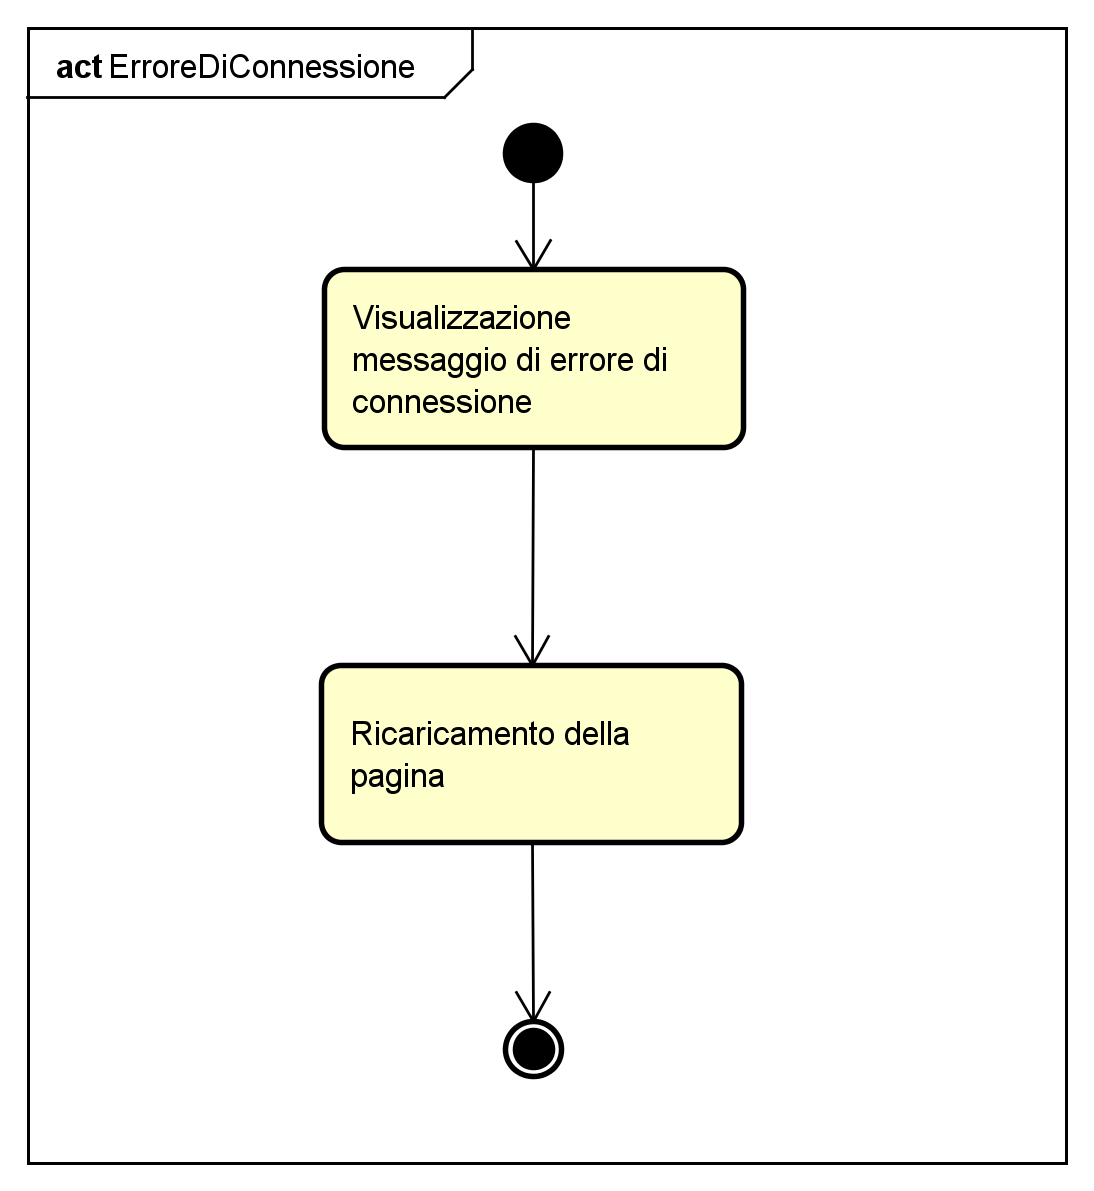
\includegraphics[scale=0.7]{img/DiagrammiDiAttivita/ErroreDiConnessione.png}
	\caption{Diagramma di attività per l'eliminazione di un nodo}
\end{figure}
\begin{figure}[H]
	\centering
	\includegraphics[width=\textwidth]{img/MockUp/m9.png}
	\caption{Mockup per gli errori di connessione}
\end{figure}
	\newpage

\section{Tracciamento}

	\subsection{Tracciamento package-requisiti}
	\def\arraystretch{1.5}
	\rowcolors{2}{D}{P}
	\begin{longtable}{p{5cm}!{\VRule[1pt]}p{2.5cm}}
		\rowcolor{I}
		\color{white} \textbf{Package} & \color{white} \textbf{Requisito} \\ 
		\endfirsthead
		\rowcolor{I}
		\color{white} \textbf{Package} & \color{white} \textbf{Requisito} \\ 
		\endhead
		ButtonsPkg & RFF14.5 \newline ROF1.3 \newline ROF1.4 \newline ROF10 \newline ROF10.1 \newline ROF11.5 \newline ROF12 \newline ROF13 \newline ROF14 \newline ROF14.3 \newline ROF14.6 \newline ROF14.7 \newline ROF15 \newline ROF16.1.11 \newline ROF16.2 \newline ROF16.3 \newline ROF18 \newline ROF19 \newline ROF19.1.11 \newline ROF19.2 \newline ROF19.3 \newline ROF2 \newline ROF20 \newline ROF22 \newline ROF3 \newline ROF4 \newline ROF4.2.1 \newline ROF4.3 \newline ROF4.4 \newline ROF45 \newline ROF46 \newline ROF48.1 \\
		ButtonsPkg & ROF5 \newline ROF5.1 \newline ROF5.2 \newline ROF6.1 \newline ROF6.10 \newline ROF6.9 \newline ROF7 \newline ROF8 \newline ROF9 \newline ROF9.1 \newline ROF9.1.1 \newline ROF9.1.3 \newline ROF9.10 \newline ROF9.2 \newline ROF9.9\\
		AnalysisPkg & ROF19 \newline ROF19.1 \newline ROF19.3 \newline ROF20 \newline ROF21 \newline ROF22 \newline ROF47\\
		ActionElementsPkg & ROF1 \newline ROF1.5 \newline ROF10 \newline ROF16 \newline ROF19 \newline ROF19.1 \newline ROF19.3 \newline ROF21 \newline ROF4 \newline ROF4.4 \newline ROF5 \newline ROF6 \newline ROF9 \newline ROF9.10\\
		ActionCreatorsPkg & RFF14.5 \newline ROF1 \newline ROF1.5 \newline ROF10 \newline ROF10.1 \newline ROF11 \newline ROF14 \newline ROF14.7 \newline ROF15 \newline ROF15.1 \newline ROF16 \newline ROF19 \newline ROF19.1 \newline ROF19.3 \newline ROF21 \newline ROF4 \newline ROF4.4 \newline ROF5 \newline ROF5.1 \newline ROF6 \newline ROF6.10 \newline ROF9 \newline ROF9.10\\
		ContentPkg & RFF11.2 \newline RFF11.3 \newline RFF11.3.1 \newline RFF11.3.1.1 \newline RFF11.3.2 \newline RFF11.6 \newline RFF11.7 \newline RFF14.4 \newline RFF14.5 \newline RFF14.5.1 \newline RFF14.5.1.1 \newline RFF14.5.2 \newline RFF14.5.2.1 \\
		ContentPkg & ROF1.2 \newline ROF1.2.1 \newline ROF1.2.1.1 \newline ROF1.2.2 \newline ROF1.2.2.1 \newline ROF1.2.3 \newline ROF1.2.3.1 \newline ROF1.2.3.2 \newline ROF1.2.3.3 \newline ROF1.2.3.4 \newline ROF1.2.3.5 \newline ROF1.2.3.6 \newline ROF1.2.4 \newline ROF1.2.4.1 \newline ROF1.2.4.2 \newline ROF1.2.4.3 \newline ROF1.2.4.4 \newline ROF1.2.5 \newline ROF1.2.5.1 \newline ROF1.2.5.2 \newline ROF1.2.6 \newline ROF1.2.6.1 \newline ROF1.2.7 \newline ROF1.2.7.1 \newline ROF1.3 \newline ROF1.4 \newline ROF1.6 \newline ROF10 \newline ROF10.2 \newline ROF11.3.2.1 \newline ROF11.4 \newline ROF12 \newline ROF13 \newline ROF14 \newline ROF14.1 \newline ROF14.2 \newline ROF15 \newline ROF16.1 \newline ROF16.1.1 \newline ROF16.1.1.1 \newline ROF16.1.2 \newline ROF16.1.2.1 \newline ROF16.1.3 \newline ROF16.1.3.1 \newline ROF16.1.3.10 \newline ROF16.1.3.11 \\
		ContentPkg & ROF16.1.3.2 \newline ROF16.1.3.3 \newline ROF16.1.3.4 \newline ROF16.1.3.5 \newline ROF16.1.3.6 \newline ROF16.1.3.7 \newline ROF16.1.3.8 \newline ROF16.1.3.9 \newline ROF16.1.4 \newline ROF16.1.4.1 \newline ROF16.1.5 \newline ROF16.1.5.1 \newline ROF16.1.6 \newline ROF16.1.6.1 \newline ROF17 \newline ROF18 \newline ROF19 \newline ROF19.1 \newline ROF19.1.1 \newline ROF19.1.1.1 \newline ROF19.1.11 \newline ROF19.1.2 \newline ROF19.1.2.1 \newline ROF19.1.3 \newline ROF19.1.3.11 \newline ROF19.1.4 \newline ROF19.1.4.1 \newline ROF19.1.5 \newline ROF19.1.5.1 \newline ROF19.1.6 \newline ROF19.1.6.1 \newline ROF19.2 \newline ROF19.4 \newline ROF2 \newline ROF20 \newline ROF22 \newline ROF3 \newline ROF4 \newline ROF4.2.1 \newline ROF4.2.2 \newline ROF4.2.2.1 \newline ROF4.2.3 \newline ROF4.2.3.6 \newline ROF4.2.4 \newline ROF4.2.4.4 \newline ROF4.2.5 \newline ROF4.2.5.2 \\
		ContentPkg & ROF4.2.6 \newline ROF4.2.6.1 \newline ROF4.2.7 \newline ROF4.2.7.1 \newline ROF4.3 \newline ROF4.4 \newline ROF42 \newline ROF43 \newline ROF44 \newline ROF45 \newline ROF46 \newline ROF5 \newline ROF5.2 \newline ROF6.1 \newline ROF6.10 \newline ROF6.12 \newline ROF6.12.1 \newline ROF6.12.1.1 \newline ROF6.3 \newline ROF6.3.1 \newline ROF6.3.2 \newline ROF6.3.3 \newline ROF6.3.4 \newline ROF6.3.5 \newline ROF6.3.6 \newline ROF6.4 \newline ROF6.5 \newline ROF6.5.2 \newline ROF6.5.2.1 \newline ROF6.5.3 \newline ROF6.5.3.1 \newline ROF6.5.4 \newline ROF6.5.4.1 \newline ROF6.6 \newline ROF6.6.2 \newline ROF6.6.2.1 \newline ROF6.7 \newline ROF6.7.2 \newline ROF6.7.2.1 \newline ROF6.8 \newline ROF6.9 \newline ROF7 \newline ROF8 \newline ROF9 \newline ROF9.1 \newline ROF9.1.1 \newline ROF9.1.3 \newline ROF9.10 \\
		ContentPkg & ROF9.11 \newline ROF9.12 \newline ROF9.12.1 \newline ROF9.12.1.1 \newline ROF9.2 \newline ROF9.3 \newline ROF9.4 \newline ROF9.5 \newline ROF9.5.2 \newline ROF9.5.2.1 \newline ROF9.5.3 \newline ROF9.5.3.1 \newline ROF9.5.4 \newline ROF9.5.4.1 \newline ROF9.6 \newline ROF9.6.2 \newline ROF9.6.2.1 \newline ROF9.7 \newline ROF9.7.2 \newline ROF9.7.2.1 \newline ROF9.8 \newline ROF9.9\\
		ReducerPkg & RFF14.5 \newline ROF1 \newline ROF1.5 \newline ROF10 \newline ROF10.1 \newline ROF11 \newline ROF11.5 \newline ROF14 \newline ROF14.1 \newline ROF14.2 \newline ROF15 \newline ROF15.1 \newline ROF16 \newline ROF19 \newline ROF19.1 \newline ROF19.3 \newline ROF21 \newline ROF4 \newline ROF4.4 \newline ROF5 \newline ROF5.1 \newline ROF6 \newline ROF6.10 \newline ROF9 \newline ROF9.10\\
		FactorySidebarPkg & ROF1 \newline ROF1.3 \newline ROF1.4 \newline ROF1.5 \newline ROF10 \newline ROF11 \newline ROF14 \newline ROF15 \newline ROF16 \newline ROF19 \newline ROF20 \newline ROF4 \newline ROF4.2 \newline ROF4.2.1 \newline ROF4.3 \newline ROF45 \newline ROF46 \newline ROF5 \newline ROF6 \newline ROF9 \newline ROF9.2 \newline ROF9.9\\
		ProcessPkg & ROF1 \newline ROF1.3 \newline ROF1.4 \newline ROF1.5 \newline ROF10 \newline ROF11 \newline ROF12 \newline ROF14 \newline ROF15 \newline ROF2 \newline ROF4 \newline ROF4.4 \newline ROF5 \newline ROF6 \newline ROF7 \newline ROF9 \newline ROF9.10\\
		MapComponentsPkg & RFF14.8 \newline RFF16.1.10 \newline RFF16.1.9 \newline RFF19.1.10 \newline RFF19.1.9 \newline RFF24.4 \newline ROF1 \newline ROF1.1 \newline ROF1.1.1 \newline ROF1.1.2 \newline ROF1.1.3 \newline ROF1.3 \newline ROF1.4 \newline ROF1.5 \newline ROF1.6 \newline ROF10 \newline ROF11 \newline ROF11.1 \newline ROF11.1.1 \newline ROF11.1.2 \newline ROF14 \newline ROF15 \newline ROF15.1 \newline ROF15.2 \newline ROF16 \newline ROF16.1.7 \newline ROF16.1.7.1 \newline ROF16.1.8 \newline ROF16.1.8.1 \newline ROF16.2 \newline ROF16.3 \newline ROF16.4 \newline ROF19.1.7 \newline ROF19.1.7.1 \newline ROF19.1.8 \newline ROF19.1.8.1 \newline ROF19.4 \newline ROF20 \newline ROF20.1 \newline ROF20.2 \newline ROF22 \newline ROF23 \newline ROF24 \newline ROF24.1 \newline ROF24.2 \newline ROF24.3 \\
		MapComponentsPkg & ROF4 \newline ROF4.1 \newline ROF4.3 \newline ROF4.5 \newline ROF42 \newline ROF43 \newline ROF44 \newline ROF47 \newline ROF48 \newline ROF5 \newline ROF6 \newline ROF6.1 \newline ROF6.11 \newline ROF6.2 \newline ROF9 \newline ROF9.1 \newline ROF9.1.1 \newline ROF9.1.3 \newline ROF9.11 \newline ROF9.2 \newline ROF9.9\\
		CallManagerPkg & ROF1 \newline ROF1.5 \newline ROF10 \newline ROF11 \newline ROF14 \newline ROF15 \newline ROF16 \newline ROF19 \newline ROF20 \newline ROF21 \newline ROF22 \newline ROF4 \newline ROF5 \newline ROF6 \newline ROF9\\
		DeGeOPViewPkg & RFF24.4 \newline RFF25 \newline RFF25.1 \newline RFF26 \newline RFF26.1 \newline ROF1 \newline ROF1.3 \newline ROF1.4 \newline ROF1.5 \newline ROF10 \newline ROF11 \newline ROF14 \newline ROF15 \newline ROF16 \newline ROF19 \newline ROF19.4 \newline ROF21 \newline ROF24 \newline ROF24.1 \newline ROF24.2 \newline ROF24.3 \newline ROF39 \newline ROF4 \newline ROF4.1.1 \newline ROF4.1.2 \newline ROF4.1.3 \newline ROF4.2 \newline ROF4.3 \newline ROF4.5 \newline ROF40 \newline ROF41 \newline ROF47 \newline ROF48 \newline ROF5 \newline ROF6 \newline ROF6.11 \newline ROF9 \newline ROF9.2 \newline ROF9.9\\
		PolygonPkg & ROF1 \newline ROF1.3 \newline ROF1.4 \newline ROF1.5 \newline ROF10 \newline ROF15 \newline ROF16 \newline ROF19 \newline ROF4 \newline ROF5\\
		StoreContentsPkg & RFF25 \newline RFF25.1 \newline RFF26 \newline RFF26.1 \newline ROF1 \newline ROF1.3 \newline ROF1.4 \newline ROF1.5 \newline ROF10 \newline ROF10.1 \newline ROF11 \newline ROF11.5 \newline ROF14 \newline ROF14.1 \newline ROF14.2 \newline ROF15 \newline ROF16 \newline ROF20 \newline ROF4 \newline ROF47 \newline ROF48 \newline ROF48.1 \newline ROF5 \newline ROF5.1 \newline ROF6 \newline ROF6.10 \newline ROF9\\
		ActionPkg & ROF11 \newline ROF14 \newline ROF15\\
		SidebarPkg & ROF1 \newline ROF1.3 \newline ROF1.4 \newline ROF1.5 \newline ROF10 \newline ROF11 \newline ROF14 \newline ROF15 \newline ROF16 \newline ROF4 \newline ROF4.3 \newline ROF5 \newline ROF6 \newline ROF9 \newline ROF9.2 \newline ROF9.9\\
		\rowcolor{white}
		\caption{Tracciamento package-requisiti}
	\end{longtable}

	\subsection{Tracciamento package-requisiti}	
	\def\arraystretch{1.5}
	\rowcolors{2}{D}{P}
	\begin{longtable}{p{2.5cm}!{\VRule[1pt]}p{5cm}}
		\rowcolor{I}
		\color{white} \textbf{Requisito} & \color{white} \textbf{Package} \\ 
		\endfirsthead
		\rowcolor{I}
		\color{white} \textbf{Requisito} & \color{white} \textbf{Package} \\ 
		\endhead
		RFF11.2 & ContentPkg\\
		RFF11.3 & ContentPkg\\
		RFF11.3.1 & ContentPkg\\
		RFF11.3.1.1 & ContentPkg\\
		RFF11.3.2 & ContentPkg\\
		RFF11.6 & ContentPkg\\
		RFF11.7 & ContentPkg\\
		RFF14.4 & ContentPkg\\
		RFF14.5 & ActionCreatorsPkg \newline ReducerPkg \newline ButtonsPkg \newline ContentPkg\\
		RFF14.5.1 & ContentPkg\\
		RFF14.5.1.1 & ContentPkg\\
		RFF14.5.2 & ContentPkg\\
		RFF14.5.2.1 & ContentPkg\\
		RFF14.8 & MapComponentsPkg\\
		RFF16.1.10 & MapComponentsPkg\\
		RFF16.1.9 & MapComponentsPkg\\
		RFF19.1.10 & MapComponentsPkg\\
		RFF19.1.9 & MapComponentsPkg\\
		RFF24.4 & DeGeOPViewPkg \newline MapComponentsPkg\\
		RFF25 & DeGeOPViewPkg \newline StoreContentsPkg\\
		RFF25.1 & DeGeOPViewPkg \newline StoreContentsPkg\\
		RFF26 & DeGeOPViewPkg \newline StoreContentsPkg\\
		RFF26.1 & DeGeOPViewPkg \newline StoreContentsPkg\\
		ROF1 & ProcessPkg \newline ActionElementsPkg \newline ActionCreatorsPkg \newline ReducerPkg \newline MapComponentsPkg \newline CallManagerPkg \newline DeGeOPViewPkg \newline PolygonPkg \newline StoreContentsPkg \newline FactorySidebarPkg \newline SidebarPkg\\
		ROF1.1 & MapComponentsPkg\\
		ROF1.1.1 & MapComponentsPkg\\
		ROF1.1.2 & MapComponentsPkg\\
		ROF1.1.3 & MapComponentsPkg\\
		ROF1.2 & ContentPkg\\
		ROF1.2.1 & ContentPkg\\
		ROF1.2.1.1 & ContentPkg\\
		ROF1.2.2 & ContentPkg\\
		ROF1.2.2.1 & ContentPkg\\
		ROF1.2.3 & ContentPkg\\
		ROF1.2.3.1 & ContentPkg\\
		ROF1.2.3.2 & ContentPkg\\
		ROF1.2.3.3 & ContentPkg\\
		ROF1.2.3.4 & ContentPkg\\
		ROF1.2.3.5 & ContentPkg\\
		ROF1.2.3.6 & ContentPkg\\
		ROF1.2.4 & ContentPkg\\
		ROF1.2.4.1 & ContentPkg\\
		ROF1.2.4.2 & ContentPkg\\
		ROF1.2.4.3 & ContentPkg\\
		ROF1.2.4.4 & ContentPkg\\
		ROF1.2.5 & ContentPkg\\
		ROF1.2.5.1 & ContentPkg\\
		ROF1.2.5.2 & ContentPkg\\
		ROF1.2.6 & ContentPkg\\
		ROF1.2.6.1 & ContentPkg\\
		ROF1.2.7 & ContentPkg\\
		ROF1.2.7.1 & ContentPkg\\
		ROF1.3 & ProcessPkg \newline MapComponentsPkg \newline DeGeOPViewPkg \newline PolygonPkg \newline StoreContentsPkg \newline SidebarPkg \newline ButtonsPkg \newline ContentPkg \newline FactorySidebarPkg\\
		ROF1.4 & ProcessPkg \newline MapComponentsPkg \newline PolygonPkg \newline StoreContentsPkg \newline DeGeOPViewPkg \newline SidebarPkg \newline ButtonsPkg \newline ContentPkg \newline FactorySidebarPkg\\
		ROF1.5 & ProcessPkg \newline ActionElementsPkg \newline ActionCreatorsPkg \newline ReducerPkg \newline CallManagerPkg \newline DeGeOPViewPkg \newline StoreContentsPkg \newline FactorySidebarPkg \newline MapComponentsPkg \newline PolygonPkg \newline SidebarPkg\\
		ROF1.6 & ContentPkg \newline MapComponentsPkg\\
		ROF10 & MapComponentsPkg \newline CallManagerPkg \newline DeGeOPViewPkg \newline StoreContentsPkg \newline ProcessPkg \newline ActionElementsPkg \newline ActionCreatorsPkg \newline ReducerPkg \newline PolygonPkg \newline SidebarPkg \newline FactorySidebarPkg \newline ButtonsPkg \newline ContentPkg\\
		ROF10.1 & ActionCreatorsPkg \newline ReducerPkg \newline StoreContentsPkg \newline ButtonsPkg\\
		ROF10.2 & ContentPkg\\
		ROF11 & MapComponentsPkg \newline CallManagerPkg \newline DeGeOPViewPkg \newline StoreContentsPkg \newline ProcessPkg \newline ActionPkg \newline ActionCreatorsPkg \newline ReducerPkg \newline FactorySidebarPkg \newline SidebarPkg\\
		ROF11.1 & MapComponentsPkg\\
		ROF11.1.1 & MapComponentsPkg\\
		ROF11.1.2 & MapComponentsPkg\\
		ROF11.3.2.1 & ContentPkg\\
		ROF11.4 & ContentPkg\\
		ROF11.5 & ReducerPkg \newline ButtonsPkg \newline StoreContentsPkg\\
		ROF12 & ProcessPkg \newline ButtonsPkg \newline ContentPkg\\
		ROF13 & ButtonsPkg \newline ContentPkg\\
		ROF14 & MapComponentsPkg \newline CallManagerPkg \newline DeGeOPViewPkg \newline StoreContentsPkg \newline ProcessPkg \newline ActionPkg \newline ActionCreatorsPkg \newline ReducerPkg \newline ButtonsPkg \newline ContentPkg \newline FactorySidebarPkg \newline SidebarPkg\\
		ROF14.1 & ReducerPkg \newline ContentPkg \newline StoreContentsPkg\\
		ROF14.2 & ReducerPkg \newline ContentPkg \newline StoreContentsPkg\\
		ROF14.3 & ButtonsPkg\\
		ROF14.6 & ButtonsPkg\\
		ROF14.7 & ActionCreatorsPkg \newline ButtonsPkg\\
		ROF15 & MapComponentsPkg \newline CallManagerPkg \newline DeGeOPViewPkg \newline StoreContentsPkg \newline ProcessPkg \newline ActionPkg \newline ActionCreatorsPkg \newline ReducerPkg \newline PolygonPkg \newline SidebarPkg \newline FactorySidebarPkg \newline ButtonsPkg \newline ContentPkg\\
		ROF15.1 & ActionCreatorsPkg \newline ReducerPkg \newline MapComponentsPkg\\
		ROF15.2 & MapComponentsPkg\\
		ROF16 & MapComponentsPkg \newline CallManagerPkg \newline DeGeOPViewPkg \newline PolygonPkg \newline StoreContentsPkg \newline FactorySidebarPkg \newline ReducerPkg \newline ActionElementsPkg \newline ActionCreatorsPkg \newline SidebarPkg\\
		ROF16.1 & ContentPkg\\
		ROF16.1.1 & ContentPkg\\
		ROF16.1.1.1 & ContentPkg\\
		ROF16.1.11 & ButtonsPkg\\
		ROF16.1.2 & ContentPkg\\
		ROF16.1.2.1 & ContentPkg\\
		ROF16.1.3 & ContentPkg\\
		ROF16.1.3.1 & ContentPkg\\
		ROF16.1.3.10 & ContentPkg\\
		ROF16.1.3.11 & ContentPkg\\
		ROF16.1.3.2 & ContentPkg\\
		ROF16.1.3.3 & ContentPkg\\
		ROF16.1.3.4 & ContentPkg\\
		ROF16.1.3.5 & ContentPkg\\
		ROF16.1.3.6 & ContentPkg\\
		ROF16.1.3.7 & ContentPkg\\
		ROF16.1.3.8 & ContentPkg\\
		ROF16.1.3.9 & ContentPkg\\
		ROF16.1.4 & ContentPkg\\
		ROF16.1.4.1 & ContentPkg\\
		ROF16.1.5 & ContentPkg\\
		ROF16.1.5.1 & ContentPkg\\
		ROF16.1.6 & ContentPkg\\
		ROF16.1.6.1 & ContentPkg\\
		ROF16.1.7 & MapComponentsPkg\\
		ROF16.1.7.1 & MapComponentsPkg\\
		ROF16.1.8 & MapComponentsPkg\\
		ROF16.1.8.1 & MapComponentsPkg\\
		ROF16.2 & ButtonsPkg \newline MapComponentsPkg\\
		ROF16.3 & ButtonsPkg \newline MapComponentsPkg\\
		ROF16.4 & MapComponentsPkg\\
		ROF17 & ContentPkg\\
		ROF18 & ButtonsPkg \newline ContentPkg\\
		ROF19 & DeGeOPViewPkg \newline PolygonPkg \newline CallManagerPkg \newline ButtonsPkg \newline ContentPkg \newline FactorySidebarPkg \newline AnalysisPkg \newline ActionElementsPkg \newline ActionCreatorsPkg \newline ReducerPkg\\
		ROF19.1 & ContentPkg \newline AnalysisPkg \newline ActionElementsPkg \newline ActionCreatorsPkg \newline ReducerPkg\\
		ROF19.1.1 & ContentPkg\\
		ROF19.1.1.1 & ContentPkg\\
		ROF19.1.11 & ButtonsPkg \newline ContentPkg\\
		ROF19.1.2 & ContentPkg\\
		ROF19.1.2.1 & ContentPkg\\
		ROF19.1.3 & ContentPkg\\
		ROF19.1.3.11 & ContentPkg\\
		ROF19.1.4 & ContentPkg\\
		ROF19.1.4.1 & ContentPkg\\
		ROF19.1.5 & ContentPkg\\
		ROF19.1.5.1 & ContentPkg\\
		ROF19.1.6 & ContentPkg\\
		ROF19.1.6.1 & ContentPkg\\
		ROF19.1.7 & MapComponentsPkg\\
		ROF19.1.7.1 & MapComponentsPkg\\
		ROF19.1.8 & MapComponentsPkg\\
		ROF19.1.8.1 & MapComponentsPkg\\
		ROF19.2 & ButtonsPkg \newline ContentPkg\\
		ROF19.3 & ButtonsPkg \newline AnalysisPkg \newline ActionElementsPkg \newline ActionCreatorsPkg \newline ReducerPkg\\
		ROF19.4 & DeGeOPViewPkg \newline ContentPkg \newline MapComponentsPkg\\
		ROF2 & ProcessPkg \newline ButtonsPkg \newline ContentPkg\\
		ROF20 & StoreContentsPkg \newline CallManagerPkg \newline MapComponentsPkg \newline AnalysisPkg \newline ButtonsPkg \newline ContentPkg \newline FactorySidebarPkg\\
		ROF20.1 & MapComponentsPkg\\
		ROF20.2 & MapComponentsPkg\\
		ROF21 & AnalysisPkg \newline ActionElementsPkg \newline ActionCreatorsPkg \newline ReducerPkg \newline DeGeOPViewPkg \newline CallManagerPkg\\
		ROF22 & AnalysisPkg \newline ButtonsPkg \newline ContentPkg \newline CallManagerPkg \newline MapComponentsPkg\\
		ROF23 & MapComponentsPkg\\
		ROF24 & DeGeOPViewPkg \newline MapComponentsPkg\\
		ROF24.1 & DeGeOPViewPkg \newline MapComponentsPkg\\
		ROF24.2 & DeGeOPViewPkg \newline MapComponentsPkg\\
		ROF24.3 & DeGeOPViewPkg \newline MapComponentsPkg\\
		ROF3 & ButtonsPkg \newline ContentPkg\\
		ROF39 & DeGeOPViewPkg\\
		ROF4 & ProcessPkg \newline ActionElementsPkg \newline ActionCreatorsPkg \newline ReducerPkg \newline MapComponentsPkg \newline CallManagerPkg \newline DeGeOPViewPkg \newline PolygonPkg \newline StoreContentsPkg \newline ButtonsPkg \newline ContentPkg \newline FactorySidebarPkg \newline SidebarPkg\\
		ROF4.1 & MapComponentsPkg\\
		ROF4.1.1 & DeGeOPViewPkg\\
		ROF4.1.2 & DeGeOPViewPkg\\
		ROF4.1.3 & DeGeOPViewPkg\\
		ROF4.2 & DeGeOPViewPkg \newline FactorySidebarPkg\\
		ROF4.2.1 & ButtonsPkg \newline ContentPkg \newline FactorySidebarPkg\\
		ROF4.2.2 & ContentPkg\\
		ROF4.2.2.1 & ContentPkg\\
		ROF4.2.3 & ContentPkg\\
		ROF4.2.3.6 & ContentPkg\\
		ROF4.2.4 & ContentPkg\\
		ROF4.2.4.4 & ContentPkg\\
		ROF4.2.5 & ContentPkg\\
		ROF4.2.5.2 & ContentPkg\\
		ROF4.2.6 & ContentPkg\\
		ROF4.2.6.1 & ContentPkg\\
		ROF4.2.7 & ContentPkg\\
		ROF4.2.7.1 & ContentPkg\\
		ROF4.3 & MapComponentsPkg \newline DeGeOPViewPkg \newline SidebarPkg \newline ButtonsPkg \newline ContentPkg \newline FactorySidebarPkg\\
		ROF4.4 & ProcessPkg \newline ActionElementsPkg \newline ActionCreatorsPkg \newline ReducerPkg \newline ButtonsPkg \newline ContentPkg\\
		ROF4.5 & DeGeOPViewPkg \newline MapComponentsPkg\\
		ROF40 & DeGeOPViewPkg\\
		ROF41 & DeGeOPViewPkg\\
		ROF42 & MapComponentsPkg \newline ContentPkg\\
		ROF43 & MapComponentsPkg \newline ContentPkg\\
		ROF44 & MapComponentsPkg \newline ContentPkg\\
		ROF45 & ButtonsPkg \newline ContentPkg \newline FactorySidebarPkg\\
		ROF46 & ButtonsPkg \newline ContentPkg \newline FactorySidebarPkg\\
		ROF47 & AnalysisPkg \newline StoreContentsPkg \newline DeGeOPViewPkg \newline MapComponentsPkg\\
		ROF48 & StoreContentsPkg \newline DeGeOPViewPkg \newline MapComponentsPkg\\
		ROF48.1 & ButtonsPkg \newline StoreContentsPkg\\
		ROF5 & ProcessPkg \newline ActionElementsPkg \newline ActionCreatorsPkg \newline ReducerPkg \newline MapComponentsPkg \newline CallManagerPkg \newline DeGeOPViewPkg \newline StoreContentsPkg \newline PolygonPkg \newline SidebarPkg \newline FactorySidebarPkg \newline ButtonsPkg \newline ContentPkg\\
		ROF5.1 & ActionCreatorsPkg \newline ReducerPkg \newline StoreContentsPkg \newline ButtonsPkg\\
		ROF5.2 & ButtonsPkg \newline ContentPkg\\
		ROF6 & MapComponentsPkg \newline CallManagerPkg \newline DeGeOPViewPkg \newline StoreContentsPkg \newline FactorySidebarPkg \newline ProcessPkg \newline ActionElementsPkg \newline ActionCreatorsPkg \newline ReducerPkg \newline SidebarPkg\\
		ROF6.1 & ButtonsPkg \newline ContentPkg \newline MapComponentsPkg\\
		ROF6.10 & ActionCreatorsPkg \newline ReducerPkg \newline ButtonsPkg \newline StoreContentsPkg \newline ContentPkg\\
		ROF6.11 & DeGeOPViewPkg \newline MapComponentsPkg\\
		ROF6.12 & ContentPkg\\
		ROF6.12.1 & ContentPkg\\
		ROF6.12.1.1 & ContentPkg\\
		ROF6.2 & MapComponentsPkg\\
		ROF6.3 & ContentPkg\\
		ROF6.3.1 & ContentPkg\\
		ROF6.3.2 & ContentPkg\\
		ROF6.3.3 & ContentPkg\\
		ROF6.3.4 & ContentPkg\\
		ROF6.3.5 & ContentPkg\\
		ROF6.3.6 & ContentPkg\\
		ROF6.4 & ContentPkg\\
		ROF6.5 & ContentPkg\\
		ROF6.5.2 & ContentPkg\\
		ROF6.5.2.1 & ContentPkg\\
		ROF6.5.3 & ContentPkg\\
		ROF6.5.3.1 & ContentPkg\\
		ROF6.5.4 & ContentPkg\\
		ROF6.5.4.1 & ContentPkg\\
		ROF6.6 & ContentPkg\\
		ROF6.6.2 & ContentPkg\\
		ROF6.6.2.1 & ContentPkg\\
		ROF6.7 & ContentPkg\\
		ROF6.7.2 & ContentPkg\\
		ROF6.7.2.1 & ContentPkg\\
		ROF6.8 & ContentPkg\\
		ROF6.9 & ButtonsPkg \newline ContentPkg\\
		ROF7 & ProcessPkg \newline ButtonsPkg \newline ContentPkg\\
		ROF8 & ButtonsPkg \newline ContentPkg\\
		ROF9 & MapComponentsPkg \newline CallManagerPkg \newline DeGeOPViewPkg \newline StoreContentsPkg \newline ButtonsPkg \newline ContentPkg \newline FactorySidebarPkg \newline ProcessPkg \newline ActionElementsPkg \newline ActionCreatorsPkg \newline ReducerPkg \newline SidebarPkg\\
		ROF9.1 & ButtonsPkg \newline ContentPkg \newline MapComponentsPkg\\
		ROF9.1.1 & ButtonsPkg \newline ContentPkg \newline MapComponentsPkg\\
		ROF9.1.3 & ButtonsPkg \newline ContentPkg \newline MapComponentsPkg\\
		ROF9.10 & ButtonsPkg \newline ContentPkg \newline ProcessPkg \newline ActionElementsPkg \newline ActionCreatorsPkg \newline ReducerPkg\\
		ROF9.11 & ContentPkg \newline MapComponentsPkg\\
		ROF9.12 & ContentPkg\\
		ROF9.12.1 & ContentPkg\\
		ROF9.12.1.1 & ContentPkg\\
		ROF9.2 & MapComponentsPkg \newline DeGeOPViewPkg \newline ButtonsPkg \newline SidebarPkg \newline ContentPkg \newline FactorySidebarPkg\\
		ROF9.3 & ContentPkg\\
		ROF9.4 & ContentPkg\\
		ROF9.5 & ContentPkg\\
		ROF9.5.2 & ContentPkg\\
		ROF9.5.2.1 & ContentPkg\\
		ROF9.5.3 & ContentPkg\\
		ROF9.5.3.1 & ContentPkg\\
		ROF9.5.4 & ContentPkg\\
		ROF9.5.4.1 & ContentPkg\\
		ROF9.6 & ContentPkg\\
		ROF9.6.2 & ContentPkg\\
		ROF9.6.2.1 & ContentPkg\\
		ROF9.7 & ContentPkg\\
		ROF9.7.2 & ContentPkg\\
		ROF9.7.2.1 & ContentPkg\\
		ROF9.8 & ContentPkg\\
		ROF9.9 & MapComponentsPkg \newline DeGeOPViewPkg \newline ButtonsPkg \newline SidebarPkg \newline ContentPkg \newline FactorySidebarPkg\\
		\rowcolor{white}
		\caption{Tracciamento requisito-packages}
	\end{longtable}
	
	\subsection{Tracciamento classi-requisiti}
	\def\arraystretch{1.5}
	\rowcolors{2}{D}{P}
	\begin{longtable}{p{5cm}!{\VRule[1pt]}p{2.5cm}}
		\rowcolor{I}
		\color{white} \textbf{Classe} & \color{white} \textbf{Requisito} \\ 
		\endfirsthead
		\rowcolor{I}
		\color{white} \textbf{Classe} & \color{white} \textbf{Requisito} \\ 
		\endhead
		AbstractAnalysisButtons & ROF48.1\\
		Analysis & ROF21 \newline ROF22 \newline ROF47\\
		AnalysisAction & ROF21\\
		AnalysisActionCreator & ROF21\\
		AnalysisButtons & ROF22 \newline ROF45 \newline ROF46\\
		AnalysisContent & ROF22 \newline ROF45 \newline ROF46\\
		AnalysisReducer & ROF21\\
		AnalysisSidebarFactory & ROF45 \newline ROF46\\
		Asset & ROF1 \newline ROF1.3 \newline ROF1.4 \newline ROF1.5 \newline ROF2 \newline ROF4 \newline ROF4.4 \newline ROF5\\
		AssetAction & ROF1 \newline ROF1.5 \newline ROF4 \newline ROF4.4 \newline ROF5\\
		AssetActionCreator & ROF1 \newline ROF1.5 \newline ROF4 \newline ROF4.4 \newline ROF5 \newline ROF5.1 \newline ROF6.10\\
		AssetReducer & ROF1 \newline ROF1.5 \newline ROF4 \newline ROF4.4 \newline ROF5 \newline ROF5.1 \newline ROF6.10\\
		ButtonWrapper & RFF19.1.9 \newline ROF1 \newline ROF1.3 \newline ROF1.4 \newline ROF10 \newline ROF11 \newline ROF14 \newline ROF15 \newline ROF16 \newline ROF4 \newline ROF4.3 \newline ROF5 \newline ROF6 \newline ROF9 \newline ROF9.2 \newline ROF9.9\\
		CallManager & ROF1 \newline ROF1.5 \newline ROF10 \newline ROF11 \newline ROF14 \newline ROF15 \newline ROF16 \newline ROF4 \newline ROF5 \newline ROF6 \newline ROF9\\
		ConcreteDeGeOPViewBuilder & ROF1 \newline ROF1.3 \newline ROF1.5 \newline ROF10 \newline ROF11 \newline ROF14 \newline ROF15 \newline ROF16 \newline ROF19 \newline ROF21 \newline ROF4 \newline ROF4.3 \newline ROF5 \newline ROF6 \newline ROF9 \newline ROF9.2 \newline ROF9.9\\
		ConcretePolygon & ROF1.3 \newline ROF1.4\\
		ConcretePolygonFactory & ROF1 \newline ROF16 \newline ROF19 \newline ROF4\\
		Coordinate & ROF1.3 \newline ROF1.4\\
		Customer & ROF1 \newline ROF1.3 \newline ROF1.4 \newline ROF1.5 \newline ROF10 \newline ROF11 \newline ROF14 \newline ROF15 \newline ROF16 \newline ROF20 \newline ROF4 \newline ROF47 \newline ROF48 \newline ROF48.1 \newline ROF5 \newline ROF6 \newline ROF9\\
		DataFromServer & ROF1 \newline ROF11 \newline ROF14 \newline ROF16 \newline ROF21 \newline ROF22 \newline ROF4 \newline ROF6\\
		DataToServer & ROF1 \newline ROF1.5 \newline ROF10 \newline ROF11 \newline ROF14 \newline ROF15 \newline ROF16 \newline ROF19 \newline ROF20 \newline ROF21 \newline ROF4 \newline ROF5 \newline ROF6 \newline ROF9\\
		DeGeOPView & RFF24.4 \newline RFF25 \newline RFF25.1 \newline RFF26 \newline RFF26.1 \newline ROF1 \newline ROF1.3 \newline ROF1.4 \newline ROF1.5 \newline ROF10 \newline ROF11 \newline ROF14 \newline ROF15 \newline ROF16 \newline ROF19.4 \newline ROF21 \newline ROF24 \newline ROF24.1 \newline ROF24.2 \newline ROF24.3 \newline ROF39 \newline ROF4 \newline ROF4.1.1 \newline ROF4.1.2 \newline ROF4.1.3 \newline ROF4.2 \newline ROF4.3 \newline ROF4.5 \newline ROF40 \newline ROF41 \newline ROF47 \newline ROF48 \newline ROF5 \newline ROF6 \newline ROF6.11 \newline ROF9 \newline ROF9.2 \newline ROF9.9\\
		Director & ROF1 \newline ROF1.3 \newline ROF1.4 \newline ROF1.5 \newline ROF10 \newline ROF11 \newline ROF14 \newline ROF15 \newline ROF16 \newline ROF19 \newline ROF21 \newline ROF4 \newline ROF4.3 \newline ROF5 \newline ROF6 \newline ROF9 \newline ROF9.2 \newline ROF9.9\\
		Edge & ROF1.3 \newline ROF1.4 \newline ROF10 \newline ROF11 \newline ROF12 \newline ROF14 \newline ROF15 \newline ROF5\\
		EdgeAction & ROF11 \newline ROF14 \newline ROF15\\
		EdgeActionCreator & RFF14.5 \newline ROF11 \newline ROF14 \newline ROF14.7 \newline ROF15 \newline ROF15.1\\
		EdgeReducer & RFF14.5 \newline ROF11 \newline ROF11.5 \newline ROF14 \newline ROF14.1 \newline ROF14.2 \newline ROF15 \newline ROF15.1\\
		EditAssetButtons & ROF4 \newline ROF4.2.1 \newline ROF4.4\\
		EditAssetContent & ROF4 \newline ROF4.2.1 \newline ROF4.2.2 \newline ROF4.2.2.1 \newline ROF4.2.3 \newline ROF4.2.3.6 \newline ROF4.2.4 \newline ROF4.2.4.4 \newline ROF4.2.5 \newline ROF4.2.5.2 \newline ROF4.2.6 \newline ROF4.2.6.1 \newline ROF4.2.7 \newline ROF4.2.7.1 \newline ROF4.4\\
		EditAssetSidebarFactory & ROF4 \newline ROF4.2 \newline ROF4.2.1\\
		EditEdgeButtons & RFF14.5 \newline ROF14 \newline ROF14.3 \newline ROF14.7\\
		EditEdgeContent & RFF14.4 \newline RFF14.5 \newline RFF14.5.1 \newline RFF14.5.1.1 \newline RFF14.5.2 \newline RFF14.5.2.1 \newline ROF14\\
		EditEdgeSidebarFactory & ROF14\\
		EditNodeButtons & ROF9 \newline ROF9.1.1 \newline ROF9.1.3 \newline ROF9.10 \newline ROF9.2 \newline ROF9.9\\
		EditNodeContent & ROF1.2.3.3 \newline ROF14.1 \newline ROF14.2 \newline ROF9 \newline ROF9.1.1 \newline ROF9.1.3 \newline ROF9.10 \newline ROF9.11 \newline ROF9.12 \newline ROF9.12.1 \newline ROF9.12.1.1 \newline ROF9.3 \newline ROF9.4 \newline ROF9.5 \newline ROF9.5.2 \newline ROF9.5.2.1 \newline ROF9.5.3 \newline ROF9.5.3.1 \newline ROF9.5.4 \newline ROF9.5.4.1 \newline ROF9.6 \newline ROF9.6.2 \newline ROF9.6.2.1 \newline ROF9.7 \newline ROF9.7.2 \newline ROF9.7.2.1 \newline ROF9.8\\
		EditNodeSidebarFactory & ROF9\\
		EditScenarioButtons & ROF19 \newline ROF19.1.11 \newline ROF19.2 \newline ROF19.3\\
		EditScenarioContent & ROF19 \newline ROF19.1 \newline ROF19.1.1 \newline ROF19.1.1.1 \newline ROF19.1.2 \newline ROF19.1.2.1 \newline ROF19.1.3 \newline ROF19.1.3.11 \newline ROF19.1.4 \newline ROF19.1.4.1 \newline ROF19.1.5 \newline ROF19.1.5.1 \newline ROF19.1.6 \newline ROF19.1.6.1 \newline ROF19.4\\
		EditScenarioSidebarFactory & ROF19\\
		Exit & ROF1.3 \newline ROF1.4 \newline ROF10 \newline ROF5\\
		InsertAssetButtons & ROF6.10\\
		InsertAssetContent & ROF1.2 \newline ROF1.2.1 \newline ROF1.2.1.1 \newline ROF1.2.2 \newline ROF1.2.2.1 \newline ROF1.2.3 \newline ROF1.2.3.1 \newline ROF1.2.3.2 \newline ROF1.2.3.3 \newline ROF1.2.3.4 \newline ROF1.2.3.5 \newline ROF1.2.3.6 \newline ROF1.2.4 \newline ROF1.2.4.1 \newline ROF1.2.4.2 \newline ROF1.2.4.3 \newline ROF1.2.4.4 \newline ROF1.2.5 \newline ROF1.2.5.1 \newline ROF1.2.5.2 \newline ROF1.2.6 \newline ROF1.2.6.1 \newline ROF1.2.7 \newline ROF1.2.7.1 \newline ROF1.6\\
		InsertAssetSidebarFactory & ROF1 \newline ROF1.5\\
		InsertEdgeButtons & ROF11.5\\
		InsertEdgeContent & RFF11.2 \newline RFF11.3 \newline RFF11.3.1 \newline RFF11.3.1.1 \newline RFF11.3.2 \newline RFF11.6 \newline RFF11.7 \newline ROF1.6 \newline ROF11.3.2.1 \newline ROF11.4\\
		InsertEdgeSidebarFactory & ROF11\\
		InsertNodeButtons & ROF6.1 \newline ROF6.10 \newline ROF6.9 \newline ROF9.1\\
		InsertNodeContent & ROF6.1 \newline ROF6.12 \newline ROF6.12.1 \newline ROF6.12.1.1 \newline ROF6.3 \newline ROF6.3.1 \newline ROF6.3.2 \newline ROF6.3.3 \newline ROF6.3.4 \newline ROF6.3.5 \newline ROF6.3.6 \newline ROF6.4 \newline ROF6.5 \newline ROF6.5.2 \newline ROF6.5.2.1 \newline ROF6.5.3 \newline ROF6.5.3.1 \newline ROF6.5.4 \newline ROF6.5.4.1 \newline ROF6.6 \newline ROF6.6.2 \newline ROF6.6.2.1 \newline ROF6.7 \newline ROF6.7.2 \newline ROF6.7.2.1 \newline ROF6.8 \newline ROF9.1\\
		InsertNodeSidebarFactory & ROF6\\
		InsertScenarioButtons & ROF16.1.11 \newline ROF16.2 \newline ROF16.3\\
		InsertScenarioContent & ROF10.2 \newline ROF11.4 \newline ROF16.1 \newline ROF16.1.1 \newline ROF16.1.1.1 \newline ROF16.1.2 \newline ROF16.1.2.1 \newline ROF16.1.3 \newline ROF16.1.3.1 \newline ROF16.1.3.10 \newline ROF16.1.3.11 \newline ROF16.1.3.2 \newline ROF16.1.3.3 \newline ROF16.1.3.4 \newline ROF16.1.3.5 \newline ROF16.1.3.6 \newline ROF16.1.3.7 \newline ROF16.1.3.8 \newline ROF16.1.3.9 \newline ROF16.1.4 \newline ROF16.1.4.1 \newline ROF16.1.5 \newline ROF16.1.5.1 \newline ROF16.1.6 \newline ROF16.1.6.1\\
		InsertScenarioSidebarFactory & ROF16\\
		Machine & ROF1.3 \newline ROF1.4 \newline ROF10 \newline ROF5\\
		MapWrapper & RFF16.1.10 \newline RFF16.1.9 \newline RFF19.1.10 \newline RFF19.1.9 \newline RFF24.4 \newline ROF1 \newline ROF1.1 \newline ROF1.1.1 \newline ROF1.1.2 \newline ROF1.1.3 \newline ROF1.3 \newline ROF1.5 \newline ROF10 \newline ROF11 \newline ROF11.1 \newline ROF11.1.1 \newline ROF11.1.2 \newline ROF14 \newline ROF15 \newline ROF16 \newline ROF16.1.7 \newline ROF16.1.7.1 \newline ROF16.1.8 \newline ROF16.1.8.1 \newline ROF16.2 \newline ROF16.3 \newline ROF19.1.7 \newline ROF19.1.7.1 \newline ROF19.1.8 \newline ROF19.1.8.1 \newline ROF24 \newline ROF24.1 \newline ROF24.2 \newline ROF24.3 \newline ROF4 \newline ROF4.1 \newline ROF4.3 \newline ROF42 \newline ROF43 \newline ROF44 \newline ROF5 \newline ROF6 \newline ROF6.1 \newline ROF6.2 \\
		MapWrapper & ROF9 \newline ROF9.1 \newline ROF9.1.1 \newline ROF9.1.3 \newline ROF9.2 \newline ROF9.9\\
		MessageWrapper & RFF14.8 \newline ROF1 \newline ROF1.3 \newline ROF1.5 \newline ROF1.6 \newline ROF10 \newline ROF11 \newline ROF14 \newline ROF15 \newline ROF15.1 \newline ROF15.2 \newline ROF16 \newline ROF16.4 \newline ROF19.4 \newline ROF20 \newline ROF20.1 \newline ROF22 \newline ROF23 \newline ROF4 \newline ROF4.3 \newline ROF4.5 \newline ROF47 \newline ROF48 \newline ROF5 \newline ROF6 \newline ROF6.11 \newline ROF9 \newline ROF9.11 \newline ROF9.2 \newline ROF9.9\\
		Node & ROF1.3 \newline ROF1.4 \newline ROF10 \newline ROF6 \newline ROF7 \newline ROF9 \newline ROF9.10\\
		NodeAction & ROF10 \newline ROF6 \newline ROF9 \newline ROF9.10\\
		NodeActionCreator & ROF10 \newline ROF10.1 \newline ROF6 \newline ROF9 \newline ROF9.10\\
		NodeReducer & ROF10 \newline ROF10.1 \newline ROF6 \newline ROF9 \newline ROF9.10\\
		Polygon & ROF1 \newline ROF1.5 \newline ROF10 \newline ROF15 \newline ROF16 \newline ROF19 \newline ROF4 \newline ROF5\\
		PolygonFactory & ROF19\\
		PolygonOperationWrapper & RFF16.1.10 \newline RFF16.1.9 \newline ROF1 \newline ROF1.1 \newline ROF1.1.2 \newline ROF1.5 \newline ROF10 \newline ROF15 \newline ROF16 \newline ROF16.1.7.1 \newline ROF16.1.8 \newline ROF16.1.8.1 \newline ROF19.1.7 \newline ROF19.1.8 \newline ROF20.2 \newline ROF4 \newline ROF4.1 \newline ROF5\\
		Process & ROF1.3 \newline ROF1.4 \newline ROF10 \newline ROF15 \newline ROF5\\
		Queue & ROF1.3 \newline ROF1.4 \newline ROF10 \newline ROF15 \newline ROF5\\
		Reducer & RFF14.5 \newline ROF1 \newline ROF1.5 \newline ROF10 \newline ROF10.1 \newline ROF11 \newline ROF11.5 \newline ROF14 \newline ROF14.1 \newline ROF14.2 \newline ROF15 \newline ROF15.1 \newline ROF16 \newline ROF4 \newline ROF5 \newline ROF5.1 \newline ROF6 \newline ROF6.10 \newline ROF9\\
		Resource & ROF1.3 \newline ROF1.4 \newline ROF10 \newline ROF15 \newline ROF5\\
		Scenario & ROF19 \newline ROF19.1 \newline ROF19.3 \newline ROF20\\
		ScenarioAction & ROF16 \newline ROF19 \newline ROF19.1 \newline ROF19.3\\
		ScenarioActionCreator & ROF16 \newline ROF19 \newline ROF19.1 \newline ROF19.3\\
		ScenarioReducer & ROF16 \newline ROF19 \newline ROF19.1 \newline ROF19.3\\
		Sidebar & ROF1 \newline ROF1.3 \newline ROF1.4 \newline ROF1.5 \newline ROF10 \newline ROF11 \newline ROF14 \newline ROF15 \newline ROF16 \newline ROF4 \newline ROF4.3 \newline ROF5 \newline ROF6 \newline ROF9 \newline ROF9.2 \newline ROF9.9\\
		SidebarFacade & ROF1 \newline ROF1.3 \newline ROF1.4 \newline ROF1.5 \newline ROF10 \newline ROF11 \newline ROF14 \newline ROF15 \newline ROF16 \newline ROF4 \newline ROF4.3 \newline ROF5 \newline ROF6 \newline ROF9 \newline ROF9.2 \newline ROF9.9\\
		Source & ROF1.3 \newline ROF1.4 \newline ROF10 \newline ROF15 \newline ROF5\\
		StoreDeGeOP & RFF25 \newline RFF25.1 \newline RFF26 \newline RFF26.1 \newline ROF1.3 \newline ROF1.4 \newline ROF10 \newline ROF10.1 \newline ROF11.5 \newline ROF14.1 \newline ROF14.2 \newline ROF15 \newline ROF20 \newline ROF47 \newline ROF48 \newline ROF48.1 \newline ROF5 \newline ROF5.1 \newline ROF6.10\\
		TransportEdge & ROF1.3 \newline ROF1.4 \newline ROF10 \newline ROF15 \newline ROF5\\
		ViewAssetButtons & ROF2 \newline ROF3 \newline ROF5.1 \newline ROF5.2 \newline ROF6.10\\
		ViewAssetContent & ROF2 \newline ROF3 \newline ROF42 \newline ROF5.2 \newline ROF6.10\\
		ViewAssetSidebarFactory & ROF5\\
		ViewEdgeButtons & ROF12 \newline ROF13 \newline ROF14.6\\
		ViewEdgeContent & ROF12 \newline ROF13 \newline ROF44\\
		ViewEdgeSidebarFactory & ROF15\\
		ViewNodeButtons & ROF10.1 \newline ROF7 \newline ROF8\\
		ViewNodeContent & ROF10.2 \newline ROF43 \newline ROF7 \newline ROF8\\
		ViewNodeSidebarFactory & ROF10\\
		ViewScenarioButtons & ROF1.3 \newline ROF1.4 \newline ROF10 \newline ROF15 \newline ROF18 \newline ROF20 \newline ROF4.3 \newline ROF5 \newline ROF6.10 \newline ROF6.9 \newline ROF9.2 \newline ROF9.9\\
		ViewScenarioContent & ROF1.3 \newline ROF1.4 \newline ROF10 \newline ROF15 \newline ROF17 \newline ROF18 \newline ROF19.1.11 \newline ROF19.2 \newline ROF20 \newline ROF4.3 \newline ROF5 \newline ROF6.10 \newline ROF6.9 \newline ROF9.2 \newline ROF9.9\\
		ViewScenarioSidebarFactory & ROF1.3 \newline ROF1.4 \newline ROF10 \newline ROF15 \newline ROF20 \newline ROF4.3 \newline ROF5 \newline ROF9.2 \newline ROF9.9\\
		\rowcolor{white}
		\caption{Tracciamento classe-requisiti}
	\end{longtable}
	
	\subsection{Tracciamento requisiti-classi}
	
	\def\arraystretch{1.5}
	\rowcolors{2}{D}{P}
	\begin{longtable}{p{2.5cm}!{\VRule[1pt]}p{5cm}}
		\rowcolor{I}
		\color{white} \textbf{Requisito} & \color{white} \textbf{Classe} \\ 
		\endfirsthead
		\rowcolor{I}
		\color{white} \textbf{Requisito} & \color{white} \textbf{Classe} \\ 
		\endhead
		RFF11.2 & InsertEdgeContent\\
		RFF11.3 & InsertEdgeContent\\
		RFF11.3.1 & InsertEdgeContent\\
		RFF11.3.1.1 & InsertEdgeContent\\
		RFF11.3.2 & InsertEdgeContent\\
		RFF11.6 & InsertEdgeContent\\
		RFF11.7 & InsertEdgeContent\\
		RFF14.4 & EditEdgeContent\\
		RFF14.5 & EdgeActionCreator \newline EdgeReducer \newline EditEdgeButtons \newline EditEdgeContent \newline Reducer\\
		RFF14.5.1 & EditEdgeContent\\
		RFF14.5.1.1 & EditEdgeContent\\
		RFF14.5.2 & EditEdgeContent\\
		RFF14.5.2.1 & EditEdgeContent\\
		RFF14.8 & MessageWrapper\\
		RFF16.1.10 & MapWrapper \newline PolygonOperationWrapper\\
		RFF16.1.9 & MapWrapper \newline PolygonOperationWrapper\\
		RFF19.1.10 & MapWrapper\\
		RFF19.1.9 & ButtonWrapper \newline MapWrapper\\
		RFF24.4 & DeGeOPView \newline MapWrapper\\
		RFF25 & DeGeOPView \newline StoreDeGeOP\\
		RFF25.1 & DeGeOPView \newline StoreDeGeOP\\
		RFF26 & DeGeOPView \newline StoreDeGeOP\\
		RFF26.1 & DeGeOPView \newline StoreDeGeOP\\
		ROF1 & Asset \newline AssetAction \newline AssetActionCreator \newline AssetReducer \newline ButtonWrapper \newline CallManager \newline ConcreteDeGeOPViewBuilder \newline ConcretePolygonFactory \newline Customer \newline DataFromServer \newline DataToServer \newline DeGeOPView \newline Director \newline InsertAssetSidebarFactory \newline MapWrapper \newline MessageWrapper \newline Polygon \newline PolygonOperationWrapper \newline Reducer \newline Sidebar \newline SidebarFacade\\
		ROF1.1 & MapWrapper \newline PolygonOperationWrapper\\
		ROF1.1.1 & MapWrapper\\
		ROF1.1.2 & MapWrapper \newline PolygonOperationWrapper\\
		ROF1.1.3 & MapWrapper\\
		ROF1.2 & InsertAssetContent\\
		ROF1.2.1 & InsertAssetContent\\
		ROF1.2.1.1 & InsertAssetContent\\
		ROF1.2.2 & InsertAssetContent\\
		ROF1.2.2.1 & InsertAssetContent\\
		ROF1.2.3 & InsertAssetContent\\
		ROF1.2.3.1 & InsertAssetContent\\
		ROF1.2.3.2 & InsertAssetContent\\
		ROF1.2.3.3 & EditNodeContent \newline InsertAssetContent\\
		ROF1.2.3.4 & InsertAssetContent\\
		ROF1.2.3.5 & InsertAssetContent\\
		ROF1.2.3.6 & InsertAssetContent\\
		ROF1.2.4 & InsertAssetContent\\
		ROF1.2.4.1 & InsertAssetContent\\
		ROF1.2.4.2 & InsertAssetContent\\
		ROF1.2.4.3 & InsertAssetContent\\
		ROF1.2.4.4 & InsertAssetContent\\
		ROF1.2.5 & InsertAssetContent\\
		ROF1.2.5.1 & InsertAssetContent\\
		ROF1.2.5.2 & InsertAssetContent\\
		ROF1.2.6 & InsertAssetContent\\
		ROF1.2.6.1 & InsertAssetContent\\
		ROF1.2.7 & InsertAssetContent\\
		ROF1.2.7.1 & InsertAssetContent\\
		ROF1.3 & Asset \newline ButtonWrapper \newline ConcreteDeGeOPViewBuilder \newline ConcretePolygon \newline Coordinate \newline Customer \newline DeGeOPView \newline Director \newline Edge \newline Exit \newline Machine \newline MapWrapper \newline MessageWrapper \newline Node \newline Process \newline Queue \newline Resource \newline Sidebar \newline SidebarFacade \newline Source \newline StoreDeGeOP \newline TransportEdge \newline ViewScenarioButtons \newline ViewScenarioContent \newline ViewScenarioSidebarFactory\\
		ROF1.4 & Asset \newline ButtonWrapper \newline ConcretePolygon \newline Coordinate \newline Customer \newline DeGeOPView \newline Director \newline Edge \newline Exit \newline Machine \newline Node \newline Process \newline Queue \newline Resource \newline Sidebar \newline SidebarFacade \newline Source \newline StoreDeGeOP \newline TransportEdge \newline ViewScenarioButtons \newline ViewScenarioContent \newline ViewScenarioSidebarFactory\\
		ROF1.5 & Asset \newline AssetAction \newline AssetActionCreator \newline AssetReducer \newline CallManager \newline ConcreteDeGeOPViewBuilder \newline Customer \newline DataToServer \newline DeGeOPView \newline Director \newline InsertAssetSidebarFactory \newline MapWrapper \newline MessageWrapper \newline Polygon \newline PolygonOperationWrapper \newline Reducer \newline Sidebar \newline SidebarFacade\\
		ROF1.6 & InsertAssetContent \newline InsertEdgeContent \newline MessageWrapper\\
		ROF10 & ButtonWrapper \newline CallManager \newline ConcreteDeGeOPViewBuilder \newline Customer \newline DataToServer \newline DeGeOPView \newline Director \newline Edge \newline Exit \newline Machine \newline MapWrapper \newline MessageWrapper \newline Node \newline NodeAction \newline NodeActionCreator \newline NodeReducer \newline Polygon \newline PolygonOperationWrapper \newline Process \newline Queue \newline Reducer \newline Resource \newline Sidebar \newline SidebarFacade \newline Source \newline StoreDeGeOP \newline TransportEdge \newline ViewNodeSidebarFactory \newline ViewScenarioButtons \newline ViewScenarioContent \newline ViewScenarioSidebarFactory\\
		ROF10.1 & NodeActionCreator \newline NodeReducer \newline Reducer \newline StoreDeGeOP \newline ViewNodeButtons\\
		ROF10.2 & InsertScenarioContent \newline ViewNodeContent\\
		ROF11 & ButtonWrapper \newline CallManager \newline ConcreteDeGeOPViewBuilder \newline Customer \newline DataFromServer \newline DataToServer \newline DeGeOPView \newline Director \newline Edge \newline EdgeAction \newline EdgeActionCreator \newline EdgeReducer \newline InsertEdgeSidebarFactory \newline MapWrapper \newline MessageWrapper \newline Reducer \newline Sidebar \newline SidebarFacade\\
		ROF11.1 & MapWrapper\\
		ROF11.1.1 & MapWrapper\\
		ROF11.1.2 & MapWrapper\\
		ROF11.3.2.1 & InsertEdgeContent\\
		ROF11.4 & InsertEdgeContent \newline InsertScenarioContent\\
		ROF11.5 & EdgeReducer \newline InsertEdgeButtons \newline Reducer \newline StoreDeGeOP\\
		ROF12 & Edge \newline ViewEdgeButtons \newline ViewEdgeContent\\
		ROF13 & ViewEdgeButtons \newline ViewEdgeContent\\
		ROF14 & ButtonWrapper \newline CallManager \newline ConcreteDeGeOPViewBuilder \newline Customer \newline DataFromServer \newline DataToServer \newline DeGeOPView \newline Director \newline Edge \newline EdgeAction \newline EdgeActionCreator \newline EdgeReducer \newline EditEdgeButtons \newline EditEdgeContent \newline EditEdgeSidebarFactory \newline MapWrapper \newline MessageWrapper \newline Reducer \newline Sidebar \newline SidebarFacade\\
		ROF14.1 & EdgeReducer \newline EditNodeContent \newline Reducer \newline StoreDeGeOP\\
		ROF14.2 & EdgeReducer \newline EditNodeContent \newline Reducer \newline StoreDeGeOP\\
		ROF14.3 & EditEdgeButtons\\
		ROF14.6 & ViewEdgeButtons\\
		ROF14.7 & EdgeActionCreator \newline EditEdgeButtons\\
		ROF15 & ButtonWrapper \newline CallManager \newline ConcreteDeGeOPViewBuilder \newline Customer \newline DataToServer \newline DeGeOPView \newline Director \newline Edge \newline EdgeAction \newline EdgeActionCreator \newline EdgeReducer \newline MapWrapper \newline MessageWrapper \newline Polygon \newline PolygonOperationWrapper \newline Process \newline Queue \newline Reducer \newline Resource \newline Sidebar \newline SidebarFacade \newline Source \newline StoreDeGeOP \newline TransportEdge \newline ViewEdgeSidebarFactory \newline ViewScenarioButtons \newline ViewScenarioContent \newline ViewScenarioSidebarFactory\\
		ROF15.1 & EdgeActionCreator \newline EdgeReducer \newline MessageWrapper \newline Reducer\\
		ROF15.2 & MessageWrapper\\
		ROF16 & ButtonWrapper \newline CallManager \newline ConcreteDeGeOPViewBuilder \newline ConcretePolygonFactory \newline Customer \newline DataFromServer \newline DataToServer \newline DeGeOPView \newline Director \newline InsertScenarioSidebarFactory \newline MapWrapper \newline MessageWrapper \newline Polygon \newline PolygonOperationWrapper \newline Reducer \newline ScenarioAction \newline ScenarioActionCreator \newline ScenarioReducer \newline Sidebar \newline SidebarFacade\\
		ROF16.1 & InsertScenarioContent\\
		ROF16.1.1 & InsertScenarioContent\\
		ROF16.1.1.1 & InsertScenarioContent\\
		ROF16.1.11 & InsertScenarioButtons\\
		ROF16.1.2 & InsertScenarioContent\\
		ROF16.1.2.1 & InsertScenarioContent\\
		ROF16.1.3 & InsertScenarioContent\\
		ROF16.1.3.1 & InsertScenarioContent\\
		ROF16.1.3.10 & InsertScenarioContent\\
		ROF16.1.3.11 & InsertScenarioContent\\
		ROF16.1.3.2 & InsertScenarioContent\\
		ROF16.1.3.3 & InsertScenarioContent\\
		ROF16.1.3.4 & InsertScenarioContent\\
		ROF16.1.3.5 & InsertScenarioContent\\
		ROF16.1.3.6 & InsertScenarioContent\\
		ROF16.1.3.7 & InsertScenarioContent\\
		ROF16.1.3.8 & InsertScenarioContent\\
		ROF16.1.3.9 & InsertScenarioContent\\
		ROF16.1.4 & InsertScenarioContent\\
		ROF16.1.4.1 & InsertScenarioContent\\
		ROF16.1.5 & InsertScenarioContent\\
		ROF16.1.5.1 & InsertScenarioContent\\
		ROF16.1.6 & InsertScenarioContent\\
		ROF16.1.6.1 & InsertScenarioContent\\
		ROF16.1.7 & MapWrapper\\
		ROF16.1.7.1 & MapWrapper \newline PolygonOperationWrapper\\
		ROF16.1.8 & MapWrapper \newline PolygonOperationWrapper\\
		ROF16.1.8.1 & MapWrapper \newline PolygonOperationWrapper\\
		ROF16.2 & InsertScenarioButtons \newline MapWrapper\\
		ROF16.3 & InsertScenarioButtons \newline MapWrapper\\
		ROF16.4 & MessageWrapper\\
		ROF17 & ViewScenarioContent\\
		ROF18 & ViewScenarioButtons \newline ViewScenarioContent\\
		ROF19 & ConcreteDeGeOPViewBuilder \newline ConcretePolygonFactory \newline DataToServer \newline Director \newline EditScenarioButtons \newline EditScenarioContent \newline EditScenarioSidebarFactory \newline Polygon \newline PolygonFactory \newline Scenario \newline ScenarioAction \newline ScenarioActionCreator \newline ScenarioReducer\\
		ROF19.1 & EditScenarioContent \newline Scenario \newline ScenarioAction \newline ScenarioActionCreator \newline ScenarioReducer\\
		ROF19.1.1 & EditScenarioContent\\
		ROF19.1.1.1 & EditScenarioContent\\
		ROF19.1.11 & EditScenarioButtons \newline ViewScenarioContent\\
		ROF19.1.2 & EditScenarioContent\\
		ROF19.1.2.1 & EditScenarioContent\\
		ROF19.1.3 & EditScenarioContent\\
		ROF19.1.3.11 & EditScenarioContent\\
		ROF19.1.4 & EditScenarioContent\\
		ROF19.1.4.1 & EditScenarioContent\\
		ROF19.1.5 & EditScenarioContent\\
		ROF19.1.5.1 & EditScenarioContent\\
		ROF19.1.6 & EditScenarioContent\\
		ROF19.1.6.1 & EditScenarioContent\\
		ROF19.1.7 & MapWrapper \newline PolygonOperationWrapper\\
		ROF19.1.7.1 & MapWrapper\\
		ROF19.1.8 & MapWrapper \newline PolygonOperationWrapper\\
		ROF19.1.8.1 & MapWrapper\\
		ROF19.2 & EditScenarioButtons \newline ViewScenarioContent\\
		ROF19.3 & EditScenarioButtons \newline Scenario \newline ScenarioAction \newline ScenarioActionCreator \newline ScenarioReducer\\
		ROF19.4 & DeGeOPView \newline EditScenarioContent \newline MessageWrapper\\
		ROF2 & Asset \newline ViewAssetButtons \newline ViewAssetContent\\
		ROF20 & Customer \newline DataToServer \newline MessageWrapper \newline Scenario \newline StoreDeGeOP \newline ViewScenarioButtons \newline ViewScenarioContent \newline ViewScenarioSidebarFactory\\
		ROF20.1 & MessageWrapper\\
		ROF20.2 & PolygonOperationWrapper\\
		ROF21 & Analysis \newline AnalysisAction \newline AnalysisActionCreator \newline AnalysisReducer \newline ConcreteDeGeOPViewBuilder \newline DataFromServer \newline DataToServer \newline DeGeOPView \newline Director\\
		ROF22 & Analysis \newline AnalysisButtons \newline AnalysisContent \newline DataFromServer \newline MessageWrapper\\
		ROF23 & MessageWrapper\\
		ROF24 & DeGeOPView \newline MapWrapper\\
		ROF24.1 & DeGeOPView \newline MapWrapper\\
		ROF24.2 & DeGeOPView \newline MapWrapper\\
		ROF24.3 & DeGeOPView \newline MapWrapper\\
		ROF3 & ViewAssetButtons \newline ViewAssetContent\\
		ROF39 & DeGeOPView\\
		ROF4 & Asset \newline AssetAction \newline AssetActionCreator \newline AssetReducer \newline ButtonWrapper \newline CallManager \newline ConcreteDeGeOPViewBuilder \newline ConcretePolygonFactory \newline Customer \newline DataFromServer \newline DataToServer \newline DeGeOPView \newline Director \newline EditAssetButtons \newline EditAssetContent \newline EditAssetSidebarFactory \newline MapWrapper \newline MessageWrapper \newline Polygon \newline PolygonOperationWrapper \newline Reducer \newline Sidebar \newline SidebarFacade\\
		ROF4.1 & MapWrapper \newline PolygonOperationWrapper\\
		ROF4.1.1 & DeGeOPView\\
		ROF4.1.2 & DeGeOPView\\
		ROF4.1.3 & DeGeOPView\\
		ROF4.2 & DeGeOPView \newline EditAssetSidebarFactory\\
		ROF4.2.1 & EditAssetButtons \newline EditAssetContent \newline EditAssetSidebarFactory\\
		ROF4.2.2 & EditAssetContent\\
		ROF4.2.2.1 & EditAssetContent\\
		ROF4.2.3 & EditAssetContent\\
		ROF4.2.3.6 & EditAssetContent\\
		ROF4.2.4 & EditAssetContent\\
		ROF4.2.4.4 & EditAssetContent\\
		ROF4.2.5 & EditAssetContent\\
		ROF4.2.5.2 & EditAssetContent\\
		ROF4.2.6 & EditAssetContent\\
		ROF4.2.6.1 & EditAssetContent\\
		ROF4.2.7 & EditAssetContent\\
		ROF4.2.7.1 & EditAssetContent\\
		ROF4.3 & ButtonWrapper \newline ConcreteDeGeOPViewBuilder \newline DeGeOPView \newline Director \newline MapWrapper \newline MessageWrapper \newline Sidebar \newline SidebarFacade \newline ViewScenarioButtons \newline ViewScenarioContent \newline ViewScenarioSidebarFactory\\
		ROF4.4 & Asset \newline AssetAction \newline AssetActionCreator \newline AssetReducer \newline EditAssetButtons \newline EditAssetContent\\
		ROF4.5 & DeGeOPView \newline MessageWrapper\\
		ROF40 & DeGeOPView\\
		ROF41 & DeGeOPView\\
		ROF42 & MapWrapper \newline ViewAssetContent\\
		ROF43 & MapWrapper \newline ViewNodeContent\\
		ROF44 & MapWrapper \newline ViewEdgeContent\\
		ROF45 & AnalysisButtons \newline AnalysisContent \newline AnalysisSidebarFactory\\
		ROF46 & AnalysisButtons \newline AnalysisContent \newline AnalysisSidebarFactory\\
		ROF47 & Analysis \newline Customer \newline DeGeOPView \newline MessageWrapper \newline StoreDeGeOP\\
		ROF48 & Customer \newline DeGeOPView \newline MessageWrapper \newline StoreDeGeOP\\
		ROF48.1 & AbstractAnalysisButtons \newline Customer \newline StoreDeGeOP\\
		ROF5 & Asset \newline AssetAction \newline AssetActionCreator \newline AssetReducer \newline ButtonWrapper \newline CallManager \newline ConcreteDeGeOPViewBuilder \newline Customer \newline DataToServer \newline DeGeOPView \newline Director \newline Edge \newline Exit \newline Machine \newline MapWrapper \newline MessageWrapper \newline Polygon \newline PolygonOperationWrapper \newline Process \newline Queue \newline Reducer \newline Resource \newline Sidebar \newline SidebarFacade \newline Source \newline StoreDeGeOP \newline TransportEdge \newline ViewAssetSidebarFactory \newline ViewScenarioButtons \newline ViewScenarioContent \newline ViewScenarioSidebarFactory\\
		ROF5.1 & AssetActionCreator \newline AssetReducer \newline Reducer \newline StoreDeGeOP \newline ViewAssetButtons\\
		ROF5.2 & ViewAssetButtons \newline ViewAssetContent\\
		ROF6 & ButtonWrapper \newline CallManager \newline ConcreteDeGeOPViewBuilder \newline Customer \newline DataFromServer \newline DataToServer \newline DeGeOPView \newline Director \newline InsertNodeSidebarFactory \newline MapWrapper \newline MessageWrapper \newline Node \newline NodeAction \newline NodeActionCreator \newline NodeReducer \newline Reducer \newline Sidebar \newline SidebarFacade\\
		ROF6.1 & InsertNodeButtons \newline InsertNodeContent \newline MapWrapper\\
		ROF6.10 & AssetActionCreator \newline AssetReducer \newline InsertAssetButtons \newline InsertNodeButtons \newline Reducer \newline StoreDeGeOP \newline ViewAssetButtons \newline ViewAssetContent \newline ViewScenarioButtons \newline ViewScenarioContent\\
		ROF6.11 & DeGeOPView \newline MessageWrapper\\
		ROF6.12 & InsertNodeContent\\
		ROF6.12.1 & InsertNodeContent\\
		ROF6.12.1.1 & InsertNodeContent\\
		ROF6.2 & MapWrapper\\
		ROF6.3 & InsertNodeContent\\
		ROF6.3.1 & InsertNodeContent\\
		ROF6.3.2 & InsertNodeContent\\
		ROF6.3.3 & InsertNodeContent\\
		ROF6.3.4 & InsertNodeContent\\
		ROF6.3.5 & InsertNodeContent\\
		ROF6.3.6 & InsertNodeContent\\
		ROF6.4 & InsertNodeContent\\
		ROF6.5 & InsertNodeContent\\
		ROF6.5.2 & InsertNodeContent\\
		ROF6.5.2.1 & InsertNodeContent\\
		ROF6.5.3 & InsertNodeContent\\
		ROF6.5.3.1 & InsertNodeContent\\
		ROF6.5.4 & InsertNodeContent\\
		ROF6.5.4.1 & InsertNodeContent\\
		ROF6.6 & InsertNodeContent\\
		ROF6.6.2 & InsertNodeContent\\
		ROF6.6.2.1 & InsertNodeContent\\
		ROF6.7 & InsertNodeContent\\
		ROF6.7.2 & InsertNodeContent\\
		ROF6.7.2.1 & InsertNodeContent\\
		ROF6.8 & InsertNodeContent\\
		ROF6.9 & InsertNodeButtons \newline ViewScenarioButtons \newline ViewScenarioContent\\
		ROF7 & Node \newline ViewNodeButtons \newline ViewNodeContent\\
		ROF8 & ViewNodeButtons \newline ViewNodeContent\\
		ROF9 & ButtonWrapper \newline CallManager \newline ConcreteDeGeOPViewBuilder \newline Customer \newline DataToServer \newline DeGeOPView \newline Director \newline EditNodeButtons \newline EditNodeContent \newline EditNodeSidebarFactory \newline MapWrapper \newline MessageWrapper \newline Node \newline NodeAction \newline NodeActionCreator \newline NodeReducer \newline Reducer \newline Sidebar \newline SidebarFacade\\
		ROF9.1 & InsertNodeButtons \newline InsertNodeContent \newline MapWrapper\\
		ROF9.1.1 & EditNodeButtons \newline EditNodeContent \newline MapWrapper\\
		ROF9.1.3 & EditNodeButtons \newline EditNodeContent \newline MapWrapper\\
		ROF9.10 & EditNodeButtons \newline EditNodeContent \newline Node \newline NodeAction \newline NodeActionCreator \newline NodeReducer\\
		ROF9.11 & EditNodeContent \newline MessageWrapper\\
		ROF9.12 & EditNodeContent\\
		ROF9.12.1 & EditNodeContent\\
		ROF9.12.1.1 & EditNodeContent\\
		ROF9.2 & ButtonWrapper \newline ConcreteDeGeOPViewBuilder \newline DeGeOPView \newline Director \newline EditNodeButtons \newline MapWrapper \newline MessageWrapper \newline Sidebar \newline SidebarFacade \newline ViewScenarioButtons \newline ViewScenarioContent \newline ViewScenarioSidebarFactory\\
		ROF9.3 & EditNodeContent\\
		ROF9.4 & EditNodeContent\\
		ROF9.5 & EditNodeContent\\
		ROF9.5.2 & EditNodeContent\\
		ROF9.5.2.1 & EditNodeContent\\
		ROF9.5.3 & EditNodeContent\\
		ROF9.5.3.1 & EditNodeContent\\
		ROF9.5.4 & EditNodeContent\\
		ROF9.5.4.1 & EditNodeContent\\
		ROF9.6 & EditNodeContent\\
		ROF9.6.2 & EditNodeContent\\
		ROF9.6.2.1 & EditNodeContent\\
		ROF9.7 & EditNodeContent\\
		ROF9.7.2 & EditNodeContent\\
		ROF9.7.2.1 & EditNodeContent\\
		ROF9.8 & EditNodeContent\\
		ROF9.9 & ButtonWrapper \newline ConcreteDeGeOPViewBuilder \newline DeGeOPView \newline Director \newline EditNodeButtons \newline MapWrapper \newline MessageWrapper \newline Sidebar \newline SidebarFacade \newline ViewScenarioButtons \newline ViewScenarioContent \newline ViewScenarioSidebarFactory\\
		\rowcolor{white}
		\caption{Tracciamento requisito-classi}
	\end{longtable}
	
	
	\appendix
	\newpage
\section{Descrizione design pattern}
\subsection{Introduzione}
I \glo{Design pattern}{design pattern} semplificano l'attività di progettazione, favorendo il riutilizzo del codice e rendendo l'architettura più manutenibile. I design pattern vengono definiti come soluzioni progettuali generali a problemi ricorrenti. Si tratta di una descrizione o dei modelli logici da applicare per la risoluzione di problemi che possono presentarsi durante la \glo{Fase}{fase} di progettazione. Esistono diversi design pattern e vengono suddivisi in base al problema da risolvere:
\begin{itemize}
	\item \textbf{pattern creazionali}: nascondono i costruttori delle classi e espongono dei metodi al loro posto. In questo modo si possono utilizzare oggetti senza sapere come sono implementati;
	\item \textbf{pattern comportamentali}: forniscono soluzione alle più comuni tipologie di interazione tra gli oggetti;
	\item \textbf{pattern architetturali}: operano ad un livello più elevato rispetto ad altri design pattern, ed esprimono schemi di base per impostare l'organizzazione strutturale di un sistema software. In questi schemi si descrivono sottosistemi predefiniti, i ruoli che essi assumono e le relazioni reciproche;
	\item \textbf{pattern strutturali}: consentono di riutilizzare degli oggetti esistenti fornendo agli utilizzatori un'interfaccia più adatta alle loro esigenze.
\end{itemize}
Sono stati utilizzati i seguenti design pattern:
\begin{itemize}
	\item Abstract Factory (creazionale);
	\item Builder (creazionale);
	\item Factory Method (creazionale);
	\item Facade (strutturale);
	\item Redux (architetturale).
\end{itemize}

Di seguito verranno mostrati i design pattern utilizzati e come vengono contestualizzati nel progetto \progetto{}. I diagrammi delle classi mostrati in queste comparazioni sono parziali e a scopo illustrativo. Per la loro visualizzazione completa si rimanda alla sezione \ref{componenti}.

\newpage
\subsection{Pattern Creazionali}
\subsubsection{Abstract Factory Method}
\paragraph{Descrizione}
Lo scopo dell'Abstract Factory Method è fornire un interfaccia per creare famiglie di oggetti correlati o dipendenti senza specificare quali siano le loro classi concrete.
In questo modo si permette che un sistema sia indipendente dall'implementazione degli oggetti concreti e che il client, attraverso l'interfaccia, utilizzi diverse famiglie di prodotti.
\\Questo pattern è utile quando:
\begin{itemize}
	\item 	si vuole un sistema indipendente da come gli oggetti vengono creati, composti e rappresentati;
	\item 	si vuole permettere la configurazione del sistema come scelta tra diverse famiglie di prodotti;
	\item 	si vuole fornire una \glo{Libreria}{libreria} di classi mostrando solo le interfacce e nascondendo le implementazioni.
\end{itemize}
\paragraph{Contestualizzazione}
Il pattern Abstract Factory Method viene utilizzato nel \glo{Package}{package} \texttt{ViewPkg} per la creazione dell'oggetto di tipo \texttt{Sidebar}.
In particolare è stato introdotto un livello in più di astrazione rispetto al design pattern comunemente conosciuto, per legare tra loro le tipologie di \texttt{Sidebar} creabili.
\texttt{AbstractSideBarFactory} e le sue cinque sottoclassi astratte:
\begin{itemize}
	\item \texttt{AbstractAssetSidebarFactory};
	 \item \texttt{AbstractNodeSidebarFactory};
	 \item \texttt{AbstractEdgeSidebarFactory};
	 \item \texttt{AbstractScenarioSidebarFactory};
	 \item \texttt{AbstractAnalysisSidebarFactory}.
\end{itemize}
dichiarano soltanto un'interfaccia per la creazione di sidebar, mentre la responsabilità della creazione effettiva delle istanze è delle sottoclassi concrete. È stato quindi definito un metodo di factory per ogni Sidebar. Le factory concrete specificano poi i propri prodotti ridefinendo per ciascuno di essi il metodo factory.
	\begin{figure}[H]
		\label{builder_compara}
		\centering
		\includegraphics[width=\textwidth]{img/absComparati.png}
		\caption{Abstract Factory ed estratto della sua contestualizzazione in \progetto}
	\end{figure}

\newpage
\subsubsection{Builder}
\paragraph{Descrizione}
Il Builder pattern, permette di separare la costruzione di un oggetto complesso dalla sua rappresentazione sicché il processo di costruzione stesso possa creare diverse rappresentazioni.
L'algoritmo per la creazione di un oggetto complesso è indipendente da come le varie parti vengono assemblate e così la separata classe builder si focalizza sulla corretta costruzione di un'istanza mentre la classe originale si concentra sul funzionamento degli oggetti. Ciò è particolarmente utile quando si vuole assicurare che un oggetto sia valido prima di istanziarlo, e che la logica di controllo non appaia nei costruttori degli oggetti. Un builder permette anche di costruire un oggetto passo-passo, cosa che si può verificare quando si fa il parsing di un testo o si ottengono i parametri da un'interfaccia interattiva.
\paragraph{Contestualizzazione}
Questo pattern viene utilizzato nel package  \texttt{ViewPkg} per la creazione di un oggetto di tipo  \texttt{DeGeOPView}.
\\E' stata creata l'interfaccia \texttt{DeGeOPViewBuilder} che definisce le operazioni che agiscono sull'elemento \texttt{DeGeOPView} che il \texttt{Director} chiederà di creare. Il  \texttt{ConcreteDeGeOPViewBuilder} sovrascriverà tali operazioni, incapsulando il modo di costruire e rappresentare l'oggetto \texttt{DeGeOPView}.
	\begin{figure}[H]
		\label{builder_compara}
		\centering
		\includegraphics[scale=0.13]{img/builderComparati.png}
		\caption{Builder e la sua contestualizzazione in \progetto}
	\end{figure}

\newpage
\subsubsection{Factory Method}
\paragraph{Descrizione}
Questo pattern permette di creare oggetti fornendo un'interfaccia per creare un oggetto, ma lascia che le sottoclassi decidano quale oggetto istanziare.
Il pattern factory può essere utilizzato quando:
\begin{itemize}
\item 
La creazione di un oggetto preclude il suo riuso senza una significativa duplicazione di codice.
\item 
La creazione di un oggetto richiede l'accesso ad informazioni o risorse che non dovrebbero essere contenute nella classe di composizione.
\item
La gestione del \glo{Ciclo di vita}{ciclo di vita} degli oggetti gestiti deve essere centralizzata in modo da assicurare un comportamento coerente all'interno dell'applicazione.
\end{itemize}
\paragraph{Contestualizzazione}
Questo pattern viene utilizzato nel package \texttt{StorePkg::PolygonPkg}. Sono state create le classi \texttt{ConcretePolygon}, che implementa l'interfaccia \texttt{Polygon}, e \texttt{ConcretePolygonFactor}y, che implementa l'interfaccia \texttt{PolygonFactory}. \texttt{PolygonFactory} espone il metodo \texttt{CreatePolygon}, che viene sovrascritto dalla sua sottoclasse \texttt{ConcretePolygonFactory} consentendo quindi ai suoi utilizzatori, \texttt{Scenario} e \texttt{\glo{Asset}{Asset}}, la creazione dell'oggetto di tipo \texttt{Polygon}.
	\begin{figure}[H]
		\label{builder_compara}
		\centering
		\includegraphics[scale=0.14]{img/factoryComparati.png}
		\caption{Factory Method e la sua contestualizzazione in \progetto}
	\end{figure}


\newpage
\subsubsection{Singleton}
\paragraph{Descrizione}
Il singleton è un design pattern creazionale che ha lo scopo di garantire la creazione di una e una sola istanza di una determinata classe e di fornire un punto di accesso globale a tale istanza.
\\Solitamente questo pattern viene implementato mettendo privato il costruttore della classe interessata e gestendo gli accessi all'oggetto con chiamate statiche per ottenere l'unico riferimento (anch'esso statico) alla classe. La creazione dell'oggetto può avvenire per un metodo di inizializzazione o la prima volta che si tenta di accedere all'istanza di classe.
\\Il Singleton pattern viene comunemente usato nell'implementazione di abstract Factory e Builder e a volte nell'implementazione di Facade od oggetti stato.
	\begin{figure}[H]
		\label{builder_compara}
		\centering
		\includegraphics[scale=0.7]{img/singleton.png}
		\caption{Diagramma del Singleton}
	\end{figure}
	
\paragraph{Contestualizzazione}
Molte classi dell'applicazione sono singleton per costruzione.
Viene riportato l'elenco delle classi singleton (il percorso è da considerarsi relativo a partire da DeGeOP::).
\begin{itemize}
	\item StorePkg::AnalysisPkg::AnalysisContainer;
	\item StorePkg::CustomerContentsPkg::Customer;
	\item StorePkg::PolygonPkg::PolygonFactory;
	\item StorePkg::PolygonPkg::ConcretePolygonFactory;
	\item ReducerPkg::Reducer;
	\item ReducerPkg::AssetReducer;
	\item ReducerPkg::NodeReducer;
	\item ReducerPkg::EdgeReducer;
	\item ReducerPkg::ScenarioReducer;
	\item ReducerPkg::AnalysisReducer;
	\item ActionCreatorPkg::AssetActionCreator;
	\item ActionCreatorPkg::NodoActionCreator;
	\item ActionCreatorPkg::EdgeActionCreator;
	\item ActionCreatorPkg::ScenarioActionCreator;
	\item ActionCreatorPkg::AnalysisActionCreator;
	\item CallManagerPkg::CallManager;
	\item CallManagerPkg::DataFromServer;
	\item CallManagerPkg::DataToServer;
	\item View::Director;
	\item View::DeGeOPViewBuilder;
	\item View::ConcreteDeGeOPView;
	\item View::MapPkg::DeGeOPView;
	\item View::MapPkg::MessageWrapper;
	\item View::MapPkg::MapWrapper;
	\item View::MapPkg::ButtonWrapper;
	\item View::MapPkg::PolygonOperationWrapper;
	\item tutte le classi contenute in View::SidebarPkg.
\end{itemize}

\newpage
\subsection{Pattern Strutturali}
\subsubsection{Facade}
\paragraph{Descrizione}
Questo design pattern ha lo scopo di fornire un'interfaccia unificata per un insieme di interfacce presenti in un sottosistema. Facade definisce un'interfaccia di livello più alto che rende il sottosistema più semplice da utilizzare.
\paragraph{Contestualizzazione}
Questo pattern viene utilizzato nel package \texttt{ViewPkg}. E' stata creata la classe \texttt{SidebarFacade}, in modo che il client \texttt{DeGeOPView} possa creare le varie tipologie di Sidebar senza la necessità di conoscere le implementazioni dell'interfaccia factory.
	\begin{figure}[H]
		\label{builder_compara}
		\centering
		\includegraphics[scale=0.15]{img/facadeComparati.png}
		\caption{Facade ed estratto della sua contestualizzazione in \progetto}
	\end{figure}


\newpage
\subsection{Pattern Architetturali}
\subsubsection{Redux}
\label{dp_redux} % non togliere!
\paragraph{Descrizione}
Il pattern proposto dalla libreria Redux comprende 3 componenti:
\begin{itemize}
	\item \textbf{\glo{Store}{Store}}: è un unico oggetto globale read-only che contiene i dati da gestire, memorizzando l'intero stato del programma;
	\item \textbf{Actions}: definiscono le azioni che si occupano di aggiornare lo Store: l'unico modo di cambiare lo Store è emettere un'azione;
	\item \textbf{\glo{Reducer}{Reducer}}: funzioni pure che, ricevuto un input uno stato e un'azione, restituiscono un nuovo stato modificato in base all'azione.
\end{itemize}
Dato uno Store e una funzione Reducer, lo stato del programma viene aggiornato in modo deterministico con i dati delle azioni.
Il vero punto di forza di Redux è la gestione del flusso di dati in modo unidirezionale. Questo significa che tutti i dati dell'applicazione seguono lo stesso flusso, rendendo la logica dell'applicazione più predicibile e facile da capire e implementare.
\paragraph{Contestualizzazione}
Questo design pattern viene utilizzato per il design dell'architettura ad alto livello, come illustrato nella sezione \nameref{descrizione_architettura} e \nameref{tecnologie}. L'intera applicazione nel suo insieme implementa questo design pattern.
\\Le classi \texttt{\glo{Action}{Action}} all'interno del package \texttt{ActionPkg} e \texttt{Reducer} all'interno di ReducerPkg implementano rispettivamente le componenti Action e Reducer di questo design pattern.
\\L'unico modo per cambiare i dati contenuti all'interno del package \texttt{StorePkg} è emettere delle Actions.
	\begin{figure}[H]
		\label{redux_compara}
		\centering
		\includegraphics[scale=0.3]{img/ComparaArch.png}
		\caption{Design pattern proposto da Redux e la sua contestualizzazione in \progetto}
	\end{figure}
\end{document}